%%
\documentclass[manuscript,acmsmall,anonymous,review,screen,nonacm=true, authorversion=true]{acmart}

%%
%% \BibTeX command to typeset BibTeX logo in the docs
\AtBeginDocument{%
  \providecommand\BibTeX{{%
    Bib\TeX}}}

%% Rights management information.  This information is sent to you
%% when you complete the rights form.  These commands have SAMPLE
%% values in them; it is your responsibility as an author to replace
%% the commands and values with those provided to you when you
%% complete the rights form.
\setcopyright{acmcopyright}
\copyrightyear{2018}
\acmYear{2018}
\acmDOI{XXXXXXX.XXXXXXX}

%% These commands are for a PROCEEDINGS abstract or paper.
\acmConference[Conference acronym 'XX]{Make sure to enter the correct
  conference title from your rights confirmation emai}{June 03--05,
  2018}{Woodstock, NY}
%%
%%  Uncomment \acmBooktitle if the title of the proceedings is different
%%  from ``Proceedings of ...''!
%%
%%\acmBooktitle{Woodstock '18: ACM Symposium on Neural Gaze Detection,
%%  June 03--05, 2018, Woodstock, NY}
\acmPrice{15.00}
\acmISBN{978-1-4503-XXXX-X/18/06}


%%
%% Submission ID.
%% Use this when submitting an article to a sponsored event. You'll
%% receive a unique submission ID from the organizers
%% of the event, and this ID should be used as the parameter to this command.
%%\acmSubmissionID{123-A56-BU3}

%%
%% For managing citations, it is recommended to use bibliography
%% files in BibTeX format.
%%
%% You can then either use BibTeX with the ACM-Reference-Format style,
%% or BibLaTeX with the acmnumeric or acmauthoryear sytles, that include
%% support for advanced citation of software artefact from the
%% biblatex-software package, also separately available on CTAN.
%%
%% Look at the sample-*-biblatex.tex files for templates showcasing
%% the biblatex styles.
%%

%%
%% The majority of ACM publications use numbered citations and
%% references.  The command \citestyle{authoryear} switches to the
%% "author year" style.
%%
%% If you are preparing content for an event
%% sponsored by ACM SIGGRAPH, you must use the "author year" style of
%% citations and references.
%% Uncommenting
%% the next command will enable that style.
%%\citestyle{acmauthoryear}
\usepackage{booktabs}   %% For formal tables:
                        %% http://ctan.org/pkg/booktabs
\usepackage{subcaption} %% For complex figures with subfigures/subcaptions
                        %% http://ctan.org/pkg/subcaption

%%%%%%%%%%%%%%%%%%%%%%%%%%%% INPUTTING SELF DEFINED COMMANDS, SELF IMPORTED PACKAGES %%%%%%%%%%%%%%%%%%%%%%%%%%%%%%%%%%%%%%%%%%
%%%%%%%%%%%%%%%%%%%%%%%%%%%%%%%%%%%%%%%%%%%%%%%%%%%%%%%%%%%%%%%%%%%%%%%%%%%%%%%%%%%%%%%%%%%%%%%%%%%%%%%%%%%%%%%%%%%%%%%%%%%%%%%%%%%%%%%%%
%%%%%%%%%%%%%%%%%%%%%%%%%%%%%%%%%%%%%%%%%%%%%%%%%%%%% COMMANDS FOR GENERAL PAPER WRITING %%%%%%%%%%%%%%%%%%%%%%%%%%%%%%%%%%%%%%%%%%%%%%%%%%%%
%%%%%%%%%%%%%%%%%%%%%%%%%%%%%%%%%%%%%%%%%%%%%%%%%%%%%%%%%%%%%%%%%%%%%%%%%%%%%%%%%%%%%%%%%%%%%%%%%%%%%%%%%%%%%%%%%%%%%%%%%%%%%%%%%%%%%%%%%


%%%%%%%%%%%%%%%%%%%%%%%%%%%% Theorem, Definition and Proof
\newtheorem{lem}{Lemma}[section]
\newtheorem{thm}{Theorem}[section]
\newtheorem{defn}{Definition}
\newtheorem{coro}{Corollary}[thm]

\newtheorem{lemma}{Lemma}
\newtheorem{corollary}{Corollary}
\newtheorem*{theorem}{Theorem}
\renewcommand\thelemma{\unskip}
\renewcommand\thecorollary{\unskip}

% \theoremstyle{remark}
% \newtheorem*{lemma}{Lemma}

\newtheorem{example}{Example}[section]

\newcommand{\completeness}[1]{{\color{blue}\textbf{[[ #1 ]]}}}
\newcommand{\caseL}[1]{\item \textbf{case: #1}\newline}
\newcommand{\subcaseL}[1]{\item \textbf{sub-case: #1}\newline}
\newcommand{\subsubcaseL}[1]{\item \textbf{subsub-case: #1}\newline}
\newcommand{\subsubsubcaseL}[1]{\item \textbf{subsubsub-case: \boldmath{#1}}\newline}

\newcommand{\blue}[1]{{\tiny \color{blue}{ #1 }}}


\let\originalleft\left
\let\originalright\right
\renewcommand{\left}{\mathopen{}\mathclose\bgroup\originalleft}
\renewcommand{\right}{\aftergroup\egroup\originalright}
\newcommand{\ts}[1]{ \llparenthesis {#1} \rrparenthesis }

\theoremstyle{definition}

\newtheorem{case}{Case}
\newtheorem{subcase}{Case}
\numberwithin{subcase}{case}
\newtheorem{subsubcase}{Case}
\numberwithin{subsubcase}{subcase}

\newtheorem{subsubsubcase}{Case}
\numberwithin{subsubsubcase}{subsubcase}
\newcommand{\st}{~.~}
\newcommand{\sthat}{~.~}

%%%%COLORS
\definecolor{periwinkle}{rgb}{0.8, 0.8, 1.0}
\definecolor{powderblue}{rgb}{0.69, 0.88, 0.9}
\definecolor{sandstorm}{rgb}{0.93, 0.84, 0.25}
\definecolor{trueblue}{rgb}{0.0, 0.45, 0.81}

\newlength\Origarrayrulewidth
% horizontal rule equivalent to \cline but with 2pt width
\newcommand{\Cline}[1]{%
 \noalign{\global\setlength\Origarrayrulewidth{\arrayrulewidth}}%
 \noalign{\global\setlength\arrayrulewidth{2pt}}\cline{#1}%
 \noalign{\global\setlength\arrayrulewidth{\Origarrayrulewidth}}%
}

% draw a vertical rule of width 2pt on both sides of a cell
\newcommand\Thickvrule[1]{%
  \multicolumn{1}{!{\vrule width 2pt}c!{\vrule width 2pt}}{#1}%
}

% draw a vertical rule of width 2pt on the left side of a cell
\newcommand\Thickvrulel[1]{%
  \multicolumn{1}{!{\vrule width 2pt}c|}{#1}%
}

% draw a vertical rule of width 2pt on the right side of a cell
\newcommand\Thickvruler[1]{%
  \multicolumn{1}{|c!{\vrule width 2pt}}{#1}%
}

\newenvironment{subproof}[1][\proofname]{%
  \renewcommand{\qedsymbol}{$\blacksquare$}%
  \begin{proof}[#1]%
}{%
  \end{proof}%
}
%%%%%%%%%%%%%%%%%%%%%%%%%%%%%%% Fonts Definition %%%%%%%%%%%%%%%%%%%%%%%%%%%
\newcommand{\omitthis}[1]{}

% Misc.
\newcommand{\etal}{\textit{et al.}}
\newcommand{\bump}{\hspace{3.5pt}}

% Text fonts
\newcommand{\tbf}[1]{\textbf{#1}}

% Math fonts
\newcommand{\mbb}[1]{\mathbb{#1}}
\newcommand{\mbf}[1]{\mathbf{#1}}
\newcommand{\mrm}[1]{\mathrm{#1}}
\newcommand{\mtt}[1]{\mathtt{#1}}
\newcommand{\mcal}[1]{\mathcal{#1}}
\newcommand{\mfrak}[1]{\mathfrak{#1}}
\newcommand{\msf}[1]{\mathsf{#1}}
\newcommand{\mscr}[1]{\mathscr{#1}}

\newcommand{\diam}{{\color{red}\diamond}}
\newcommand{\dagg}{{\color{blue}\dagger}}
\let\oldstar\star
\renewcommand{\star}{\oldstar}

\newcommand{\im}[1]{\ensuremath{#1}}

\newcommand{\kw}[1]{\im{\mathtt{#1}}}
\newcommand{\set}[1]{\im{\{{#1}\}}}

\newcommand{\mmax}{\ensuremath{\mathsf{max}}}

%%%%%%%%%%%%%%%%%%%%%%%%%%%%%%% Blocks Definition %%%%%%%%%%%%%%%%%%%%%%%%%%%
\tikzstyle{decision} = [diamond, draw, fill=blue!20, 
    text width=4.5em, text badly centered, node distance=3cm, inner sep=0pt]
% \tikzstyle{block} = [rectangle, draw, fill=blue!20, 
%     text width=5em, text centered, rounded corners, minimum height=4em]
\tikzstyle{block} = [draw, very thick, fill=white, rectangle, 
    minimum height=2.5em, minimum width=6em, text centered]

\tikzstyle{line} = [draw, -latex']
\tikzstyle{cloud} = [draw, ellipse,fill=red!20, node distance=3cm,    minimum height=2em]

\tikzstyle{vecArrow} = [thick, decoration={markings,mark=at position
  1 with {\arrow[semithick]{open triangle 60}}},
  double distance=1.4pt, shorten >= 5.5pt,
  preaction = {decorate},
  postaction = {draw,line width=1.4pt, white,shorten >= 4.5pt}]
\tikzstyle{innerWhite} = [semithick, white,line width=1.4pt, shorten >= 4.5pt]



%%%%%%%%%%%%%%%%%%%%%%%%%%%%%%%%%%%%%%%%%%%%%%%%%%%%%%%%%%%%%%%%%%%%%%%%%%%%%%%%%%%%%%%%%%%%%%%%%%%%%%%%%%%%%%%%%%%%%%%%%%%%%%%%%%%%%%%%%%%%%%%%%%%%%%%%%%
%%%%%%%%%%%%%%%%%%%%%%%%%%%%%%%%%%%%%%%%%%%%%%%%%%%%%%%%%%%% Introduction %%%%%%%%%%%%%%%%%%%%%%%%%%%%%%%%%%%%%%%%%%%%%%%%%%%%%%%%%%%%%%%%
%%%%%%%%%%%%%%%%%%%%%%%%%%%%%%%%%%%%%%%%%%%%%%%%%%%%%%%%%%%%%%%%%%%%%%%%%%%%%%%%%%%%%%%%%%%%%%%%%%%%%%%%%%%%%%%%%%%%%%%%%%%%%%%%%%%%%%%%%%%%%%%%%%%%%%%%%%

\newcommand{\dist}{P}
\newcommand{\mech}{M}
\newcommand{\univ}{\mathcal{X}}
\newcommand{\anyl}{A}
\newcommand{\qrounds}{r}
\newcommand{\answer}{a}
\newcommand{\sample}{X}
\newcommand{\ex}[2]{{\ifx&#1& \mathbb{E} \else \underset{#1}{\mathbb{E}} \fi \left[#2\right]}}
\newcommand{\pr}[2]{{\ifx&#1& \mathbb{P} \else \underset{#1}{\mathbb{P}} \fi \left[#2\right]}}
\newcommand{\var}[2]{{\ifx&#1& \mathrm{Var} \else \underset{#1}{\mathrm{Var}} \fi \left[#2\right]}}
\newcommand{\eps}{\varepsilon}
\newcommand{\from}{:}
\newcommand{\sep}{ \ | \ }


%%%%%%%%%%%%%%%%%%%%%%%%%%%%%%%%%%%%%%%%%%%%%%%%%%%%%%%%%%%%%%%%%%%%%%%%%%%%%%%%%%%%%%%%%%%%%%%%%%%%%%%%%%%%%%%%%%%%%%%%%%%%%%%%%%%%%%%%%%%%%%%%%%%%%%%%%%
%%%%%%%%%%%%%%%%%%%%%%%%%%%%%%%%%%%%%%%%%%%%%%%%%%%%%%%%%%%% Query While Language %%%%%%%%%%%%%%%%%%%%%%%%%%%%%%%%%%%%%%%%%%%%%%%%%%%%%%%%%%%%%%%%
%%%%%%%%%%%%%%%%%%%%%%%%%%%%%%%%%%%%%%%%%%%%%%%%%%%%%%%%%%%%%%%%%%%%%%%%%%%%%%%%%%%%%%%%%%%%%%%%%%%%%%%%%%%%%%%%%%%%%%%%%%%%%%%%%%%%%%%%%%%%%%%%%%%%%%%%%%
% Language
\newcommand{\command}{c}
%Label
\newcommand{\lin}{\kw{in}}
\newcommand{\lex}{\kw{ex}}
% expression
\newcommand{\expr}{e}
\newcommand{\aexpr}{a}
\newcommand{\bexpr}{b}
\newcommand{\sexpr}{\ssa{\expr} }
\newcommand{\qexpr}{\psi}
\newcommand{\qval}{\alpha}
\newcommand{\query}{{\tt query}}
\newcommand{\eif}{\;\kw{if}\;}
\newcommand{\ethen}{\kw{\;then\;}}
\newcommand{\eelse}{\kw{\;else\;}} 
\newcommand{\eapp}{\;}
\newcommand{\eprojl}{\kw{fst}}
\newcommand{\eprojr}{\kw{snd}}
\newcommand{\eifvar}{\kw{ifvar}}
\newcommand{\ewhile}{\;\kw{while}\;}
\newcommand{\bop}{\;*\;}
\newcommand{\uop}{\;\circ\;}
\newcommand{\eskip}{\kw{skip}}
\newcommand{\edo}{\;\kw{do}\;}
% More unary expression operators:
\newcommand{\esign}{~\kw{sign}~}
\newcommand{\elog}{~\kw{log}~}


\newcommand{\emax}{~\kw{max}~}
\newcommand{\emin}{~\kw{min}~}


%%%%%%%%%% Extended
\newcommand{\efun}{~\kw{fun}~}
\newcommand{\ecall}{~\kw{call}~}


% Domains
\newcommand{\qdom}{\mathcal{QD}}
\newcommand{\memdom}{\mathcal{M}}
\newcommand{\dbdom}{\mathcal{DB}}
\newcommand{\cdom}{\mathcal{C}}
\newcommand{\ldom}{\mathcal{L}}

\newcommand{\emap}{~\kw{map}~}
\newcommand{\efilter}{~\kw{filter}~}

%configuration
\newcommand{\config}[1]{\langle #1 \rangle}
\newcommand{\ematch}{\kw{match}}
\newcommand{\clabel}[1]{\left[ #1 \right]}

\newcommand{\etrue}{\kw{true}}
\newcommand{\efalse}{\kw{false}}
\newcommand{\econst}{c}
\newcommand{\eop}{\delta}
\newcommand{\efix}{\mathop{\kw{fix}}}
\newcommand{\elet}{\mathop{\kw{let}}}
\newcommand{\ein}{\mathop{ \kw{in}} }
\newcommand{\eas}{\mathop{ \kw{as}} }
\newcommand{\enil}{\kw{nil}}
\newcommand{\econs}{\mathop{\kw{cons}}}
\newcommand{\term}{t}
\newcommand{\return}{\kw{return}}
\newcommand{\bernoulli}{\kw{bernoulli}}
\newcommand{\uniform}{\kw{uniform}}
\newcommand{\app}[2]{\mathrel{ {#1} \, {#2} }}


% Operational Semantics
\newcommand{\env}{\rho}
\newcommand{\rname}[1]{\textsf{\small{#1}}}
\newcommand{\aarrow}{\Downarrow_a}
\newcommand{\barrow}{\Downarrow_b}
\newcommand{\earrow}{\Downarrow_e}
\newcommand{\qarrow}{\Downarrow_q}
\newcommand{\cmd}{c}
\newcommand{\node}{N}
\newcommand{\assign}[2]{ \mathrel{ #1  \leftarrow #2 } }


%%%%%%%%%%%%%%%%%%%%%%%%%%%%%%%%%%%%%%%%%%%%%%%%%%%%%%%%%%%%%%%%%%%%%%%% Trace and Events %%%%%%%%%%%%%%%%%%%%%%%%%%%%%%%%%%%%%%%%
%%%%%%%%%%%%%%%%%%%%%%%%%%%%%%%%%%%%%%%%%%%%%%%%%%%%%%%%%%%%%%%%%%%%%% Trace 
%%%%%%%% annotated query
\newcommand{\aq}{\kw{aq}}
\newcommand{\qtrace}{\kw{qt}}
%annotated variables
\newcommand{\av}{\kw{av}}
\newcommand{\vtrace}{\kw{\tau}}
\newcommand{\ostrace}{{\kw{\tau}}}
\newcommand{\posttrace}{{\kw{\tau}}}



%%%%%%%%%%%%%%%%%traces
\newcommand{\tdom}{\mathcal{T}^{+\infty}}
\newcommand{\trace}{\kw{\tau}}
\newcommand{\ftdom}{\mathcal{T}^{+}}
\newcommand{\inftdom}{\mathcal{T}^{\infty}}

% \newcommand{\vcounter}{\kw{\zeta}}
\newcommand{\vcounter}{\kw{cnt}}

\newcommand{\postevent}{{\kw{\epsilon}}}


\newcommand{\event}{\kw{\epsilon}}
\newcommand{\eventset}{\mathcal{E}}
\newcommand{\eventin}{\in_{\kw{e}}}
\newcommand{\eventeq}{=_{\kw{e}}}
\newcommand{\eventneq}{\neq_{\kw{e}}}
\newcommand{\eventgeq}{\geq_{\kw{e}}}
\newcommand{\eventlt}{<_{\kw{e}}}
\newcommand{\eventleq}{\leq_{\kw{e}}}
\newcommand{\eventdep}{\mathsf{DEP_{\kw{e}}}}
\newcommand{\asn}{\kw{{asn}}}
\newcommand{\test}{\kw{{test}}}
\newcommand{\ctl}{\kw{{ctl}}}

\newcommand{\sig}{\kw{sig}}
\newcommand{\sigeq}{=_{\sig}}
\newcommand{\signeq}{\neq_{\sig}}
\newcommand{\notsigin}{\notin_{\sig}}
\newcommand{\sigin}{\in_{\sig}}
\newcommand{\sigdiff}{\kw{Diff}_{\sig}}
\newcommand{\action}{\kw{act}}
\newcommand{\diff}{\kw{Diff}}
\newcommand{\seq}{\kw{seq}}
\newcommand{\sdiff}{\kw{Diff}_{\seq}}

\newcommand{\tracecat}{{\scriptscriptstyle ++}}
\newcommand{\traceadd}{{\small ::}}

\newcommand{\ism}{\kw{ism}}
\newcommand{\ismdiff}{\kw{Diff}_{\sig}}
\newcommand{\ismeq}{=_{\ism}}
\newcommand{\ismneq}{\neq_{\ism}}
\newcommand{\notismin}{\notin_{\ism}}
\newcommand{\ismin}{\in_{\ism}}

%operations on the trace and Annotated Query
\newcommand{\projl}[1]{\kw{\pi_{l}(#1)}}
\newcommand{\projr}[1]{\kw{\pi_{r}(#1)}}

% operations on annotated query, i.e., aq
\newcommand{\aqin}{\in_{\kw{aq}}}
\newcommand{\aqeq}{=_{\kw{aq}}}
\newcommand{\aqneq}{\neq_{\kw{aq}}}
\newcommand{\aqgeq}{\geq_{\kw{aq}}}

% operations on annotated variables, i.e., av
\newcommand{\avin}{\in_{\kw{av}}}
\newcommand{\aveq}{=_{\kw{av}}}
\newcommand{\avneq}{\neq_{\kw{av}}}
\newcommand{\avgeq}{\geq_{\kw{av}}}
\newcommand{\avlt}{<_{\kw{av}}}

% adaptivity
\newcommand{\adap}{\kw{adap}}
\newcommand{\ddep}[1]{\kw{depth}_{#1}}
\newcommand{\nat}{\mathbb{N}}
\newcommand{\natb}{\nat_{\bot}}
\newcommand{\natbi}{\natb^\infty}
\newcommand{\nnatA}{Z}
\newcommand{\nnatB}{m}
\newcommand{\nnatbA}{s}
\newcommand{\nnatbB}{t}
\newcommand{\nnatbiA}{q}
\newcommand{\nnatbiB}{r}


%%%%%%%%%%%%%%%%%%%%%%%%%%%%%%%%%%%%%%%%%%%%%%%%%%%%%%%%%%%%%%%%%%%%%%%%%%%%%%%%%%%%%%%%%%%%%%%%%%%%%%%%%%%%%%%%%%%%%%%%%%%%%%%%%%%%%%%%%%%%%%%%%%%%%%%%%%
%%%%%%%%%%%%%%%%%%%%%%%%%%%%%%%%%%%%%%%%%%%%%%%%%%%%%%%%%%%% Semantic Definition %%%%%%%%%%%%%%%%%%%%%%%%%%%%%%%%%%%%%%%%%%%%%%%%%%%%%%%%%%%%%%%%
%%%%%%%%%%%%%%%%%%%%%%%%%%%%%%%%%%%%%%%%%%%%%%%%%%%%%%%%%%%%%%%%%%%%%%%%%%%%%%%%%%%%%%%%%%%%%%%%%%%%%%%%%%%%%%%%%%%%%%%%%%%%%%%%%%%%%%%%%%%%%%%%%%%%%%%%%%

%%%%%%%%%%%%%%%%%%%%%%%%%%%%%%%%% Semantics Based Dependency, Graph and Adaptivity 
\newcommand{\paths}{\mathcal{PATH}}
\newcommand{\walks}{\mathcal{WK}}
\newcommand{\progwalks}{\mathcal{WK}^{\kw{est}}}

\newcommand{\len}{\kw{len}}
\newcommand{\lvar}{\mathbb{LV}}
\newcommand{\avar}{\mathbb{AV}}
\newcommand{\qvar}{\mathbb{QV}}
\newcommand{\qdep}{\mathsf{DEP_{q}}}
\newcommand{\vardep}{\mathsf{DEP_{var}}}
\newcommand{\avdep}{\mathsf{DEP_{\av}}}
\newcommand{\finitewalk}{\kw{fw}}
\newcommand{\pfinitewalk}{\kw{fwp}}
\newcommand{\dep}{\mathsf{DEP}}

\newcommand{\llabel}{\iota}
\newcommand{\entry}{\kw{entry}}
\newcommand{\tlabel}{\mathbb{TL}}

\newcommand{\traceG}{\kw{{G_{trace}}}}
\newcommand{\traceV}{\kw{{V_{trace}}}}
\newcommand{\traceE}{\kw{{E_{trace}}}}
\newcommand{\traceF}{\kw{{Q_{trace}}}}
\newcommand{\traceW}{\kw{{W_{trace}}}}

%%%%%%%%%%%%%%%%%%%%%%%%%%%%%%%%%%%%%%%%%%%%%%%%%%%%%%%%%%%%%%%%%%%%%%%%%%%%%%%%%%%%%%%%%%%%%%%%%%%%%%%%%%%%%%%%%%%%%%%%%%%%%%%%%%%%%%%%%%%%%%%%%%%%%%%%%%
%%%%%%%%%%%%%%%%%%%%%%%%%%%%%%%%%%%%%%%%%%%%%%%%%%%%%%%%%%%% Static Program Analysis %%%%%%%%%%%%%%%%%%%%%%%%%%%%%%%%%%%%%%%%%%%%%%%%%%%%%%%%%%%%%%%%
%%%%%%%%%%%%%%%%%%%%%%%%%%%%%%%%%%%%%%%%%%%%%%%%%%%%%%%%%%%%%%%%%%%%%%%%%%%%%%%%%%%%%%%%%%%%%%%%%%%%%%%%%%%%%%%%%%%%%%%%%%%%%%%%%%%%%%%%%%%%%%%%%%%%%%%%%%

%Static Adaptivity Definition:
\newcommand{\flowsto}{\kw{flowsTo}}
\newcommand{\live}{\kw{RD}}

%Analysis Algorithms and Graphs
\newcommand{\weight}{\mathsf{W}}
\newcommand{\green}[1]{{ \color{green} #1 } }

\newcommand{\func}[2]{\mathsf{AD}(#1) \to (#2)}
\newcommand{\varCol}{\bf{VetxCol}}
\newcommand{\graphGen}{\bf{FlowGen}}
\newcommand{\progG}{\kw{{G_{est}}}}
\newcommand{\progV}{\kw{{V_{est}}}}
\newcommand{\progE}{\kw{{E_{est}}}}
\newcommand{\progF}{\kw{{Q_{est}}}}
\newcommand{\progW}{\kw{{W_{est}}}}
\newcommand{\progA}{{\kw{A_{est}}}}

\newcommand{\midG}{\kw{{G_{mid}}}}
\newcommand{\midV}{\kw{{V_{mid}}}}
\newcommand{\midE}{\kw{{E_{mid}}}}
\newcommand{\midF}{\kw{{Q_{mid}}}}



\newcommand{\sccgraph}{\kw{G^{SCC}}}
\newcommand{\sccG}{\kw{{G_{scc}}}}
\newcommand{\sccV}{\kw{{V_{scc}}}}
\newcommand{\sccE}{\kw{{E_{scc}}}}
\newcommand{\sccF}{\kw{{Q_{scc}}}}
\newcommand{\sccW}{\kw{{W_{scc}}}}


\newcommand{\visit}{\kw{visit}}

\newcommand{\flag}{\kw{F}}
\newcommand{\Mtrix}{\kw{M}}
\newcommand{\rMtrix}{\kw{RM}}
\newcommand{\lMtrix}{\kw{LM}}
\newcommand{\vertxs}{\kw{V}}
\newcommand{\qvertxs}{\kw{QV}}
\newcommand{\qflag}{\kw{Q}}
\newcommand{\edges}{\kw{E}}
\newcommand{\weights}{\kw{W}}
\newcommand{\qlen}{\len^{\tt q}}
\newcommand{\pwalks}{\mathcal{WK}_{\kw{p}}}

\newcommand{\rb}{\mathsf{RechBound}}
\newcommand{\pathsearch}{\mathsf{AdaptSearch}}

%program abstraction
\newcommand{\abst}[1]{\kw{abs}{#1}}
\newcommand{\absexpr}{\abst{\kw{expr}}}
% \newcommand{\absevent}{\stackrel{\scriptscriptstyle{\alpha}}{\event{}}}
\newcommand{\absevent}{\hat{\event{}}}
\newcommand{\absfinal}{\abst{\kw{final}}}
\newcommand{\absinit}{\abst{\kw{init}}}
\newcommand{\absflow}{\abst{\kw{trace}}}
\newcommand{\absG}{\abst{\kw{G}}}
\newcommand{\absV}{\abst{\kw{V}}}
\newcommand{\absE}{\abst{\kw{E}}}
\newcommand{\absF}{\abst{\kw{F}}}
\newcommand{\absW}{\abst{\kw{W}}}
\newcommand{\locbound}{\kw{locb}}
\newcommand{\absdom}{\mathcal{ADOM}}

\newcommand{\inpvar}{\vardom_{\kw{in}}}
\newcommand{\grdvar}{\vardom_{\kw{guard}}}
\newcommand{\vardom}{\mathcal{V}}
\newcommand{\inpvardom}{\mathcal{V}_{\kw{\lin}}}
\newcommand{\scexprdom}{\mathcal{A}_{\kw{sc}}}
\newcommand{\inpexprdom}{\mathcal{A}_{\lin}}
\newcommand{\scvardom}{\mathcal{SC}}
\newcommand{\valuedom}{\mathcal{VAL}}
\newcommand{\scexpr}{{\kw{A_{sc}}}}


\newcommand{\absclr}{{\kw{TB}}}
\newcommand{\varinvar}{{\kw{VB}}}
\newcommand{\init}{\kw{init}}
\newcommand{\constdom}{\mathcal{SC}}
\newcommand{\dcdom}{\mathcal{DC}}
\newcommand{\reset}{\kw{re}}
\newcommand{\resetchain}{\kw{rechain}}
\newcommand{\inc}{\kw{inc}}
\newcommand{\dec}{\kw{dec}}
\newcommand{\booldom}{\mathcal{B}}
\newcommand{\incrs}{\kw{increase}}




%%%%%%%%%%%%%%%%%%%%%%%%%%%%%%%%%%%%%%%%%%%%%%%%%%%%%%%%%%%%%%%%%%%%%%%%%%%%%%%%%%%%%%%%%%%%%%%%%%%%%%%%%%%%%%%%%%%%%%%%%%%%%%%%%%%%%%%%%%%%%%%%%%%%%%%%%%
%%%%%%%%%%%%%%%%%%%%%%%%%%%%%%%%%%%%%%%%%%%%%%%%%%%%%%%%%%%%%%%%%%%%%%% author comments in draft mode %%%%%%%%%%%%%%%%%%%%%%%%%%%%%%%%%%%%%%%%%%%%%%%%%%%%%%%%%%%%%%%%%%%%%%
%%%%%%%%%%%%%%%%%%%%%%%%%%%%%%%%%%%%%%%%%%%%%%%%%%%%%%%%%%%%%%%%%%%%%%%%%%%%%%%%%%%%%%%%%%%%%%%%%%%%%%%%%%%%%%%%%%%%%%%%%%%%%%%%%%%%%%%%%%%%%%%%%%%%%%%%%%

\newif\ifdraft
%\draftfalse
\drafttrue

\newcommand{\todo}[1]{{\color{red}\textbf{[[ #1 ]]}}}
% \newcommand{\todo}[1]{#1}
\newcommand{\todomath}[1]{{\scriptstyle \color{red}\mathbf{[[ #1 ]]}}}


\ifdraft
% Jiawen
\newcommand{\jl}[1]{\textcolor[rgb]{.00,0.00,1.00}{[JL: #1]}}
% \newcommand{\jl}[1]{#1}
\newcommand{\jlside}[1]{\marginpar{\tiny \sf \textcolor[rgb]{.00,0.80,0.00}{[jl: #1]}}}
% Deepak
\newcommand{\dg}[1]{\textcolor[rgb]{.00,0.80,0.00}{[DG: #1]}}
\newcommand{\dgside}[1]{\marginpar{\tiny \sf \textcolor[rgb]{.00,0.80,0.00}{[DG: #1]}}}
% Marco
\newcommand{\mg}[1]{\textcolor[rgb]{.80,0.00,0.00}{[MG: #1]}}
\newcommand{\mgside}[1]{\marginpar{\tiny \sf \textcolor[rgb]{.80,0.00,0.00}{[MG: #1]}}}
% Weihao
\newcommand{\wq}[1]{\textcolor[rgb]{.00,0.80,0.00}{[WQ: #1]}}
\newcommand{\wqside}[1]{\marginpar{\tiny \sf \textcolor[rgb]{.00,0.80,0.00}{[WQ: #1]}}}
\else
\newcommand{\mg}[1]{}
\newcommand{\mgside}[1]{}
\newcommand{\wq}[1]{}
\newcommand{\wqside}[1]{}
\newcommand{\rname}[1]{$\textbf{#1}$}
\fi

\newcommand{\highlight}[1]{\textcolor[rgb]{.0,0.0,1.0}{ #1}}
% \newcommand{\highlight}[1]{{ #1}}

\newcommand{\THESYSTEM}{\textsf{AdaptFun}}
%%%%%%%%%%%%%%%%%%%%%%%%%%%% FINISHING INPUTTING SELF DEFINED COMMANDS, SELF IMPORTED PACKAGES %%%%%%%%%%%%%%%%%%%%%%%%%%%%%%%%%%%%%%%%%%
%%

%% end of the preamble, start of the body of the document source.
\begin{document}

%%
%% The "title" command has an optional parameter,
%% allowing the author to define a "short title" to be used in page headers.
\title[Short Title]{Program Analysis for Adaptive Data Analysis}         %% [Short Title] is optional;

%%
%% The "author" command and its associated commands are used to define
%% the authors and their affiliations.
%% Of note is the shared affiliation of the first two authors, and the
%% "authornote" and "authornotemark" commands
%% used to denote shared contribution to the research.
%% Author with single affiliation.
\author{First1 Last1}
\authornote{with author1 note}          %% \authornote is optional;
                                        %% can be repeated if necessary
\orcid{nnnn-nnnn-nnnn-nnnn}             %% \orcid is optional
\affiliation{
  \position{Position1}
  \department{Department1}              %% \department is recommended
  \institution{Institution1}            %% \institution is required
  \streetaddress{Street1 Address1}
  \city{City1}
  \state{State1}
  \postcode{Post-Code1}
  \country{Country1}                    %% \country is recommended
}
\email{first1.last1@inst1.edu}          %% \email is recommended

%% Author with two affiliations and emails.
\author{First2 Last2}
\authornote{with author2 note}          %% \authornote is optional;
                                        %% can be repeated if necessary
\orcid{nnnn-nnnn-nnnn-nnnn}             %% \orcid is optional
\affiliation{
  \position{Position2a}
  \department{Department2a}             %% \department is recommended
  \institution{Institution2a}           %% \institution is required
  \streetaddress{Street2a Address2a}
  \city{City2a}
  \state{State2a}
  \postcode{Post-Code2a}
  \country{Country2a}                   %% \country is recommended
}
\email{first2.last2@inst2a.com}         %% \email is recommended
\affiliation{
  \position{Position2b}
  \department{Department2b}             %% \department is recommended
  \institution{Institution2b}           %% \institution is required
  \streetaddress{Street3b Address2b}
  \city{City2b}
  \state{State2b}
  \postcode{Post-Code2b}
  \country{Country2b}                   %% \country is recommended
}
\email{first2.last2@inst2b.org}         %% \email is recommended

%%
%% The abstract is a short summary of the work to be presented in the
%% article.
\begin{abstract}
Data analyses are usually designed to identify some property of the population from which the data are drawn, generalizing beyond the specific data sample. For this reason, data analyses are often designed in a way that guarantees that they produce a low generalization error.
 That is, they are designed so that the result of a data analysis run on a sample data does not differ too much from the result one would achieve by running the analysis over the entire population. 

An adaptive data analysis can be seen as a process composed by multiple queries interrogating some data, where the choice of which query to run next may rely on the results of previous queries. 
The generalization error of each individual query/analysis can be controlled by using an array of well-established statistical techniques.
However, when queries are arbitrarily composed, the different errors can propagate through the chain of different queries and bring to high generalization error. 
To address this issue, data analysts are designing several techniques that not only guarantee bounds on the generalization errors of single queries, but that also guarantee bounds on the generalization error of the composed analyses. 
The choice of which of these techniques to use, often depends on the chain of queries that an adaptive data analysis can generate.

In this work, we consider adaptive data analyses implemented as while-like programs and we design a program analysis which can help with identifying which technique to use to control their generalization error. 
More specifically, we formalize the intuitive notion of \emph{adaptivity} as a quantitative property of programs. 
We do this because the adaptivity level of a data analysis is a key measure to choose the right technique. 
Based on this definition, we design a program analysis for soundly approximating this quantity.
The program analysis generates a representation of the data analysis as a weighted dependency graph, where the weight is an upper bound on the number of times each variable can be reached, and uses a path search strategy to guarantee an upper bound on the adaptivity. 
We implement our program analysis  and show that it can help to analyze the adaptivity of several concrete data analyses with different adaptivity structures.
\end{abstract}

%%
%% The code below is generated by the tool at http://dl.acm.org/ccs.cfm.
%% Please copy and paste the code instead of the example below.
%%
% \begin{CCSXML}
% <ccs2012>
%  <concept>
%   <concept_id>10010520.10010553.10010562</concept_id>
%   <concept_desc>Computer systems organization~Embedded systems</concept_desc>
%   <concept_significance>500</concept_significance>
%  </concept>
%  <concept>
%   <concept_id>10010520.10010575.10010755</concept_id>
%   <concept_desc>Computer systems organization~Redundancy</concept_desc>
%   <concept_significance>300</concept_significance>
%  </concept>
%  <concept>
%   <concept_id>10010520.10010553.10010554</concept_id>
%   <concept_desc>Computer systems organization~Robotics</concept_desc>
%   <concept_significance>100</concept_significance>
%  </concept>
%  <concept>
%   <concept_id>10003033.10003083.10003095</concept_id>
%   <concept_desc>Networks~Network reliability</concept_desc>
%   <concept_significance>100</concept_significance>
%  </concept>
% </ccs2012>
% \end{CCSXML}

% \ccsdesc[500]{Computer systems organization~Embedded systems}
% \ccsdesc[300]{Computer systems organization~Redundancy}
% \ccsdesc{Computer systems organization~Robotics}
% \ccsdesc[100]{Networks~Network reliability}

%%
%% Keywords. The author(s) should pick words that accurately describe
%% the work being presented. Separate the keywords with commas.
\keywords{Adaptive data analysis, program analysis, dependency graph}  %% \keywords are mandatory in final camera-ready submission


%% A "teaser" image appears between the author and affiliation
%% information and the body of the document, and typically spans the
%% page.
% \begin{teaserfigure}
%   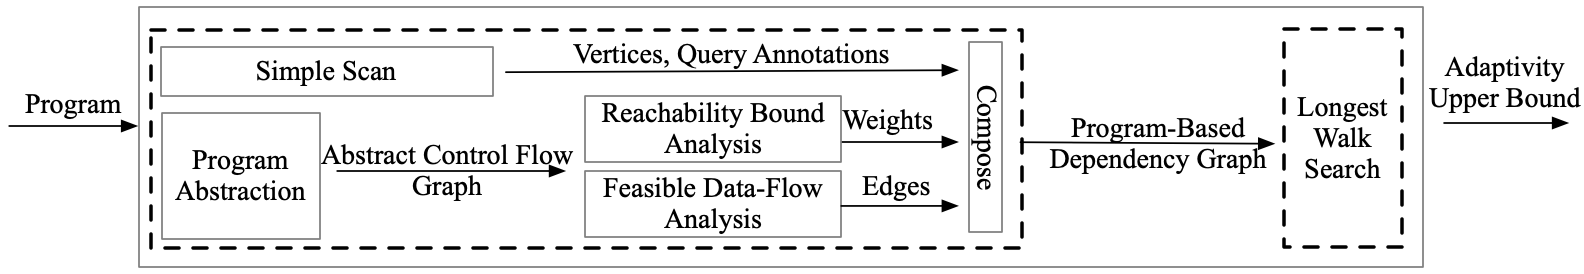
\includegraphics[width=\textwidth]{adapfun}
%   \caption{Seattle Mariners at Spring Training, 2010.}
%   \Description{Enjoying the baseball game from the third-base
%   seats. Ichiro Suzuki preparing to bat.}
%   \label{fig:teaser}
% \end{teaserfigure}

\received{20 February 2007}
\received[revised]{12 March 2009}
\received[accepted]{5 June 2009}

%%
%% This command processes the author and affiliation and title
%% information and builds the first part of the formatted document.
\maketitle

%%%%%%%%%%%%%%%%%%%%%%%%%%%%%%%%%%%%%%%%%%% Introduction and Overview %%%%%%%%%%%%%%%%%%%%%%%%%%%%%%%%%%%%%%%%%%% 
\section{Introduction}
\label{sec:intro}
% The topic, motivation, the importance of adaptivity 
Consider a dataset $X$ consisting of $n$ independent samples from some unknown population $\dist$.  How can we ensure that the conclusions drawn from $X$ \emph{generalize} to the population $\dist$?  Despite decades of research in statistics and machine learning on methods for ensuring generalization, there is an increased recognition that many scientific findings generalize poorly (e.g. 
\cite{Ioannidis05,GelmanL13}
).  While there are many reasons a conclusion might fail to generalize, one that is receiving increasing attention is \emph{adaptivity}, which occurs when the choice of method for analyzing the dataset depends on previous interactions with the same dataset~\cite{GelmanL13}.
%
 Adaptivity can arise from many common practices, such as exploratory data analysis, using the same data set for feature selection and regression, and the re-use of datasets across research projects.  Unfortunately, adaptivity invalidates traditional methods for ensuring generalization and statistical validity, which assume that the method is selected independently of the data. The misinterpretation of adaptively selected results has even been blamed for a ``statistical crisis'' in empirical science~\cite{GelmanL13}.
%  ~\cite{GelmanL13}.

\begin{figure}
    \centering
    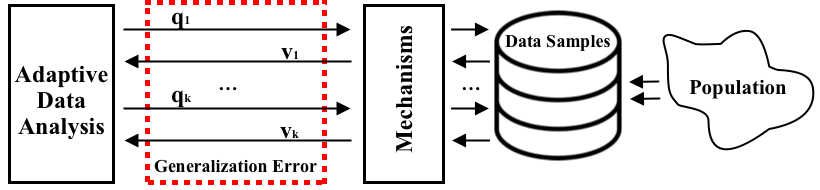
\includegraphics[width=0.7\columnwidth]{overview.png}
    \caption{Overview of our Adaptive Data Analysis model.
    We have a population that we are interested in studying, and a dataset containing individual samples from this population. 
    The adaptive data analysis we are interested in running has access to the dataset through queries of some pre-determined family (e.g., statistical or linear queries) mediated by a mechanism. 
    This mechanism uses randomization to reduce the generalization error of the queries issued to the data.}
    \label{fig:adaptivity-model-overview}
\vspace{-0.5cm}
\end{figure}

A line of work initiated by \cite{DworkFHPRR15}, \cite{HardtU14} posed the question: Can we design \emph{general-purpose} methods that ensure generalization in the presence of adaptivity, together with guarantees on their accuracy?  
The idea that has emerged in these works is to use randomization to help ensure generalization. 
Specifically, these works have proposed to mediate the access of an adaptive data analysis to the data by means of queries from some pre-determined family (we will consider here a specific family of queries often called "statistical" or "linear" queries) that are sent to a  \emph{mechanism} which uses some randomized process to guarantee that the result of the query does not depend too much on the specific
sampled dataset. 
This guarantees that the result of the queries generalizes well. This approach is described in Fig.~\ref{fig:adaptivity-model-overview}.  
This line of work has identified many new algorithmic techniques for ensuring generalization in adaptive data analysis, leading to algorithms with greater statistical power than all previous approaches. Common methods proposed by these works include, the addition of noise to the result of a query, data splitting, etc. Moreover, these works have also identified problematic strategies for adaptive analysis, showing limitations on the statistical power one can hope to achieve. Subsequent works have then further extended the methods and techniques in this approach and further extended the theoretical underpinning of this approach, e.g.~\cite{dwork2015reusable,dwork2015generalization,BassilyNSSSU16,UllmanSNSS18,FeldmanS17,jung2019new,SteinkeZ20,RogersRSSTW20}.

A key development in this line of work is that the best method for ensuring generalization in an adaptive data analysis depends to a large extent on the number of \emph{rounds of adaptivity}, the depth of the chain of queries. 
As an informal example, the program $x \leftarrow q_1(D);y \leftarrow q_2(D,x);z \leftarrow q_3(D,y)$ has three rounds of adaptivity, since $q_2$  depends on $D$ not only directly because it is one of its input but also via the result of $q_1$, which is also run on $D$, and similarly,  $q_3$ depends on $D$ directly but also via the result of $q_2$, which in turn depends on the result of $q_1$.
The works we discussed above showed that, not only does the analysis of the generalization error depend on the number of rounds, but knowing the number of rounds actually allows one to choose methods that lead to the smallest possible generalization error - we will discuss this further in Section~\ref{sec:overview}. 

For example, these works showed that when an adaptive data analysis uses a large number of rounds of adaptivity then a low generalization error can be achieved by a mechanism  
adding to the result of each query Gaussian noise scaled to the number of rounds. When instead  an adaptive data analysis uses a small number of rounds of adaptivity then a low generalization error can be achieved by using more specialized methods, such as data splitting mechanism or the reusable holdout technique from~\cite{DworkFHPRR15}.
To better understand this idea, we show in Fig.~\ref{fig:generalization_errors} three experiments showcasing these situations.
More precisely, in Fig.~\ref{fig:generalization_errors}(a) we show the results of a specific analysis\footnote{We will use formally a program implementing this analysis (Fig.~\ref{fig:overview-example}) as a running example in the rest of the paper.} with two rounds of adaptivity.
This analysis can be seen as a classifier which first runs 400 non-adaptive queries on the first 400 attributes of the data, looking for correlations between the attributes and a label, and then runs one last query which depends on all these correlations.
Without any mechanism the generalization error of the last query is pretty large, and the lower generalization error is achieved when the data-splitting method is used.
Fig.~\ref{fig:generalization_errors}(c) shows how this situation also change with the number of queries. Specifically, it shows the root mean square error of the last \emph{adaptive} query when the numbers queries varies. This also highlight the fact that different mechanisms, for the same analysis, produce results with very different generalization error.
In Fig.~\ref{fig:generalization_errors}(b), we show the results of a specific analysis\footnote{We will present this analysis formally in Section~\ref{sec:examples}.} with four hundreds rounds of adaptivity.
At each step, this analysis runs an adaptive query based on the results of the previous ones. Without any mechanism, the generalization error of most of the queries is pretty large, and this error can be lowered by using Gaussian noise. 
{\small
\begin{figure}
\centering
\begin{subfigure}{.32\textwidth}
\begin{centering}
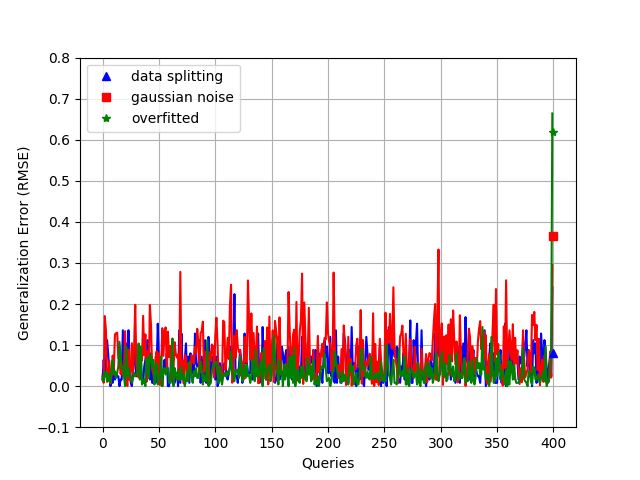
\includegraphics[width=1.0\textwidth]{tworound.png}
\caption{}
\end{centering}
\end{subfigure}
\quad
\begin{subfigure}{.32\textwidth}
\begin{centering}
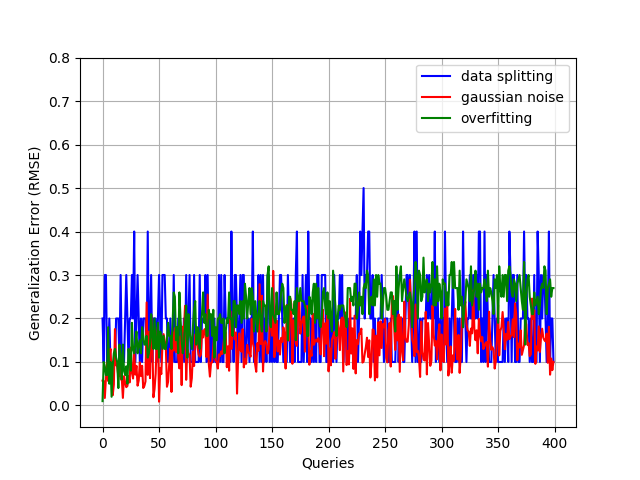
\includegraphics[width=1.0\textwidth]{multipleround.png}
\caption{}
\end{centering}
\end{subfigure}
\begin{subfigure}{.32\textwidth}
\begin{centering}
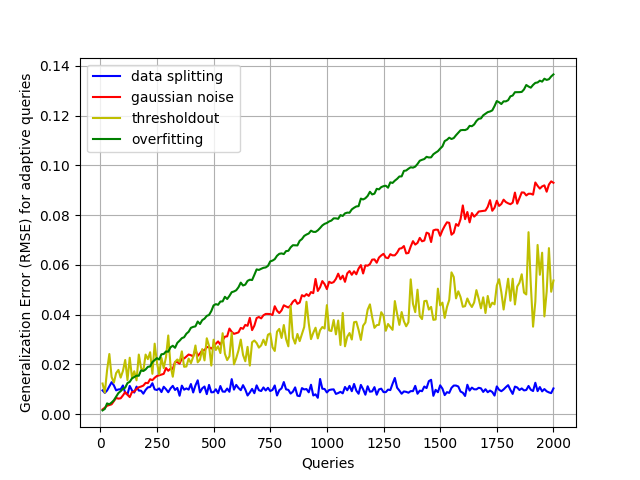
\includegraphics[width=1.0\textwidth]{twoRounds-rmse-fourmechs.png}
\caption{}
\end{centering}
\end{subfigure}
\vspace{-0.5cm}
 \caption{
 The generalization errors of two adaptive data analysis examples, under different choices of mechanisms.
 (a) Data analysis with 2 rounds adaptivity, 
 (b) Data analysis with 400 rounds adaptivity.
 (c) Same Data analysis as (a) with different query numbers.
}
\label{fig:generalization_errors}
\vspace{-0.6cm}
\end{figure}
}
%gap

This scenario motivates us to explore the design of program analysis techniques that can be used to estimate the number of \emph{rounds of adaptivity} that a program implementing a data analysis can perform. These techniques could be used to help a data analyst in the choice of the mechanism to use,
and they
could ultimately be integrated into a tool for adaptive data analysis such as the \emph{Guess and Check} framework by~\cite{RogersRSSTW20}. 

The first problem we face is \emph{how to formally define} a model for adaptive data analysis which is general enough to support the methods we discussed above and which would permit to formulate the notion of adaptivity these methods use. We take the approach of designing a programming framework for submitting queries to some \emph{mechanism} giving access to the data mediated by one of the techniques we mentioned before, e.g., adding Gaussian noise, randomly selecting a subset of the data, using the reusable holdout technique, etc. In this approach, a program models an \emph{analyst} asking a sequence of queries to the mechanism. The mechanism runs the queries on the data applying one of the methods above and returns the result to the program. The program can then use this result to decide which query to run next. Overall, we are interested in controlling the generalization of the query results returned by the mechanism, by means of the adaptivity. 

The second problem we face is \emph{how to define the adaptivity of a given program}.
Intuitively, a query $Q$ may depend on another query $P$, if there are two values that $P$ can return which affect in different ways the execution of $Q$. 
For example, as shown in \cite{dwork2015reusable}, and as we did in our example in Fig.~\ref{fig:generalization_errors}(a), one can design a machine learning algorithm for constructing a classifier which first computes each feature's correlation with the label via a sequence of queries, and then constructs the classifier based on the correlation values. If one feature's correlation changes, the classifier depending on features is also affected.  
This notion of dependency builds on the execution trace as a \emph{causal history}. In particular, we are interested in the history or provenance of a query up until this is executed, we are not then concerned about how the result is used --- except for tracking whether the result of the query may further cause some other query. This is because we focus on the generalization error of queries and not their post-processing. % 
To formalize this intuition as a quantitative program property,
we use a trace semantics recording the execution history of programs on some given input --- and we create a dependency graph, where the dependency between different variables (queries are also assigned to variables) is explicit and track which variable is associated with a query request. We then enrich this graph with weights describing the number of times each variable is evaluated in a program evaluation starting with an initial state. The adaptivity is then defined as the length of the walk visiting most query-related variables on this graph\footnote{Formally, graphs will be well-defined only for terminating programs, this will guarantee that the longest walk is finite}. In other words, we define adaptivity as a \emph{quantitative form of program dependency}.

% \jl{ 
% To define adaptivity in our programming framework, we consider a weighted dependency graph over variables assigned in the program, where each edge is built by a semantics dependency relation between these variables. The dependency relation relies on the trace semantics of our programming framework which records the execution history of programs implementing adaptive data analysis. 
% %The novelty comes from the definition of relation of dependency between nodes, which consists of the edge in the graph. For now, we can think of each node is associated with a variable, storing the value assigned to its variable 
% }
% \jl{The general idea beneath this dependency relation is that modifying the value of some variable in an execution trace will later affect the following execution trace.
% By tracking if a variable is assigned by a query or not, we are able to distinguish whether one query may depend on the other.}

The third problem we face is \emph{how to estimate the adaptivity of a given program}. 
The adaptive data analysis model we consider and our definition of adaptivity suggest that for this task we can use a  program analysis that is based on some form of dependency analysis. This analysis needs to take into consideration:
1) the fact that, in general, a query $Q$ is not a monolithic block but rather it may depend, through the use of variables and values, on other parts of the program. Hence, it needs to consider some form of data flow analysis. 
2) the fact that, in general, the decision on whether to run a query or not may depend on some other value. Hence, 
 it needs to consider some form of control flow analysis.
 3) the fact that, in general, we are not only interested in whether there is a dependency or not, but in the length of the chain of dependencies. Hence, it needs to consider some quantitative information about the program dependencies. 
 
To address these considerations and be able to estimate a sound upper bound on the adaptivity of a program, 
we develop a static program analysis algorithm, named {\THESYSTEM}, which combines data flow and control flow analysis with reachability bound analysis~\cite{GulwaniZ10}. This combination gives tighter bounds on the adaptivity of a program than the ones one would achieve by directly using the data and control flow analyses or the ones that one would achieve by directly using reachability bound analysis techniques alone. We evaluate {\THESYSTEM} on a number of examples showing that it is able to efficiently estimate precise upper bounds on the adaptivity of different programs. 
All the proofs and extended definitions can be found in the supplementary material.

To summarize, our work aims at the design of a static analysis for programs implementing adaptive analysis that can estimate their rounds of adaptivity. Specifically, our contributions are:
\begin{enumerate}
    \item A programming framework for adaptive data analyses where programs represent analysts that can query generalization-preserving mechanisms mediating the access to some data. 
    \item 
    A formal definition of the notion of adaptivity under the analyst-mechanism model. 
    This definition is built on a variable-based dependency graph that is constructed using sets of program execution traces.
    \item 
    A static program analysis algorithm {\THESYSTEM} combining data flow, control flow and  reachability bound analysis in order to provide tight bounds on the adaptivity of a program.
    \item A soundness proof of the program analysis showing that the adaptivity estimated by {\THESYSTEM} bounds the true adaptivity of the program. 
    \item An implementation of {\THESYSTEM} and an experimental evaluation of the bounds this implementation provides on several examples.
\end{enumerate}
\section{Overview}
\label{sec:overview}
\subsection{Some results in Adaptive Data Analysis}
%\wq{I think we can move this subsection into appendix. Maybe just leave theorm 1.2 and 1.3}
%\jl{I don't agree}
In Adaptive Data Analysis an \emph{analyst} is interested in studying some distribution $\dist$ over some domain $\univ$.  Following previous works~\cite{DworkFHPRR15,HardtU14,BassilyNSSSU16}, we focus on the setting where the analyst is interested in answers to \emph{statistical queries} (also known as \emph{linear queries}) over the distribution.  A statistical query is usually defined by some function $\qquery \from \univ \to [-1,1]$ (often other codomains such as $[0,1]$ or $[-R,+R]$, for some $R$, are considered).  The analyst wants to learn the \emph{population mean}, which is defined as 
$\qquery(\dist) = \ex{\sample \sim \dist}{\qquery(\sample)}$. 
%
We assume that the distribution $\dist$ can only be accessed via a set of \emph{samples} $\sample_1,\dots,\sample_n$ drawn independently and identically distributed (i.i.d.) from $\dist$.  These samples are held by a mechanism $\mech(\sample_1,\dots,\sample_n)$ who receives the query $\query$ and computes an answer 
$\answer \approx \qquery(\dist)$.
%
The na\"ive way to approximate the population mean is to use the \emph{empirical mean}, which (abusing notation) is defined as 
$\qquery(\sample_1,\dots,\sample_n) = \frac{1}{n} \sum_{i=1}^{n} \qquery(X_i)$.
However, the mechanism $M$ can adopt some methods for improving the generalization error $| a- \qquery(\dist)|$.

In this work we consider analysts that ask a sequence of $k$ queries $\qquery_1,\dots,\qquery_k$.  If the queries are all chosen in advance, independently of the answers \highlight{$a_1,\dots,a_k$} of each other, then we say they are \emph{non-adaptive}.  If the choice of each query $\qquery_j$ depends on the prefix $\qquery_1,\answer_1,\dots,\qquery_{j-1},\answer_{j-1}$ then they are \emph{fully adaptive}.  An important intermediate notion is \emph{$\qrounds$-round adaptive}, where the sequence can be partitioned into $\qrounds$ batches of non-adaptive queries.  Note that non-adaptive queries are $1$-round and fully adaptive queries are $k$-round adaptive.

We now review what is known about the problem of answering $r$-round adaptive queries.  
\begin{thm}[\cite{BassilyNSSSU16}] 
\label{thm:nonadapt-adapt}
\begin{enumerate}

\item For any distribution $\dist$, and any $k$ \emph{non-adaptive} statistical queries, \highlight{with high probablity,} 
% $$
$
\max_{j=1,\dots,k} | \answer_j - \qquery_j(\dist) | = O\left( \sqrt{\frac{\log k}{n}}  \right)
% $$
$.
%
\item For any distribution $\dist$, and  any $k$  \emph{$\qrounds$-round adaptive} statistical queries, with $\qrounds \geq 2$, \highlight{with high probablity,} the empirical mean (rounded to an appropriate number of bits of precision)\footnote{With infinite precision even two queries may give unbounded error, when the first query's result encodes the whole data.} satisfies:\\
% $$
$
\max_{j=1,\dots,k} | \answer_j - \qquery_j(\dist) | = O\left( \sqrt{\frac{k}{n}}  \right)
% $$
$
\end{enumerate}
\end{thm}
In fact, these bounds are tight (up to constant factors) which means that even allowing one extra round of adaptivity leads to an exponential increase in the generalization error, from $\log k$ to $k$.

\citet{DworkFHPRR15} and \citet{BassilyNSSSU16} showed that by using carefully calibrated Gaussian noise in order to limit the dependency of a single query on the specific data instance, one 
can actually achieve much stronger generalization error as a function of the number of queries, specifically.
\begin{thm}[\cite{DworkFHPRR15, BassilyNSSSU16}] \label{thm:gaussiannoise} For any distribution $\dist$, any $k$, any $\qrounds \geq 2$ and any \emph{$\qrounds$-round adaptive} statistical queries, if we answer queries with carefully calibrated Gaussian noise, \highlight{with high probablity,}  we have:
\begin{center}
  $
\max_{j=1,\dots,k} | \answer_j - \qquery_j(\dist) | = O\left( \frac{\sqrt[4]{k}}{\sqrt{n}}  \right)
$  
\end{center}
\end{thm}
% Notice that in order to Theorem~\ref{thm:gaussiannoise} has different quantification in that the optimal choice of mechanism depends on the number of queries.  Thus, we need to know the number of queries \emph{a priori} to choose the best mechanism.
More interestingly, \citet{DworkFHPRR15}
also gave a refined bounds that can be achieved with different mechanisms depending on the number of rounds of adaptivity.   \begin{thm}[\cite{DworkFHPRR15}] \label{thm:gaussiannoise2} For any $r$ and $k$, there exists a mechanism such that for any distribution $\dist$, and any $\qrounds \geq 2$ any \emph{$\qrounds$-round adaptive} statistical queries, \highlight{with high probablity,} it satisfies
\begin{center}
  $
\max_{j=1,\dots,k} | \answer_j - \qquery_j(\dist) | = O\left( \frac{r \sqrt{\log k}}{\sqrt{n}}  \right)
$  
\end{center}
\end{thm}
Notice that Theorem~\ref{thm:gaussiannoise2} has different quantification in that the optimal choice of mechanism depends on the number of queries {and number of rounds of adaptivity}.  This suggests that if one knows a good \emph{a priori upper bound on the number of rounds of adaptivity}, one can choose the appropriate mechanism and get a much better guarantee in terms of the generalization error.
As an example, as we can see in Fig.~\ref{fig:generalization_errors}, if we know that an algorithm is 2-rounds adaptive, we can choose data splitting as {the} mechanism, while if we know that an algorithm has many rounds of adaptivity we can choose Gaussian noise. It is worth to stress that by knowing the number of rounds of adaptivity one can also compute a concrete upper bound on the generalization error of a data analysis. This information allows one to have a quantitative, a priori, estimation of the effectiveness of a data analysis. 
This motivates us to design a static program analysis aimed at giving good \emph{a priori} upper bounds on the number of rounds of adaptivity of a program. 

{\small
\begin{figure}
\centering
\begin{subfigure}{.2\textwidth}
\begin{centering}
$
    \begin{array}{l}
    \kw{towRounds(k)} \triangleq \\
           \clabel{ \assign{a}{0}}^{0} ;
            \clabel{\assign{j}{k} }^{1} ; \\
            \ewhile ~ \clabel{j > 0}^{2} ~ \edo ~ \\
            \Big(
             \clabel{\assign{x}{\query(\chi[j] \cdot \chi[k])} }^{3}  ; \\
             \clabel{\assign{j}{j-1}}^{4} ;\\
            \clabel{\assign{a}{x + a}}^{5}       \Big);\\
            \clabel{\assign{l}{\query(\chi[k]*a)} }^{6}\\
        \end{array}
$
\caption{}
\end{centering}
\end{subfigure}
\begin{subfigure}{.4\textwidth}
%}
\qquad
\begin{centering}
\begin{tikzpicture}[scale=\textwidth/16cm,samples=250]
\draw[] (0, 10) circle (0pt) node
{{ $a^0: {}^{\lambda \trace_0. 1}_{0}$}};
\draw[] (0, 7) circle (0pt) node
{\textbf{$x^3: {}^{\lambda \trace_0. \env(\trace_0) k}_{1}$}};
\draw[] (0, 4) circle (0pt) node {{ $a^5: {}^{\lambda \trace_0. \env(\trace_0) k}_{0}$}};
\draw[] (0, 1) circle (0pt) node
{{ $l^6: {}^{\lambda \trace_0. 1}_{1}$}};
% Counter Variables
\draw[] (8, 9) circle (0pt) node {\textbf{$j^1: {}^{\lambda \trace_0. 1}_{0}$}};
\draw[] (8, 6) circle (0pt) node {{ $j^4: {}^{\lambda \trace_0. \env(\trace_0) k}_{0}$}};
%
% Value Dependency Edges:
\draw[ ultra thick, -latex, densely dotted,] (0, 1.5)  -- (0, 3.5) ;
\draw[ ultra thick, -latex, densely dotted,] (0, 4.5)  -- (0, 6.5) ;
\draw[ thick, -latex] (0, 4.5)  to  [out=-230,in=230]  (0, 9.5) ;
\draw[ thick, -Straight Barb] (1.5, 3.8) arc (120:-200:1);
\draw[ thick, -Straight Barb] (9, 6.5) arc (150:-150:1);
\draw[ thick, -latex] (8, 6.5)  -- (8, 8.5) ;
\draw[ thick, -latex] (0, 1.5)  to  [out=-230,in=230]  (0, 9.5) ;
% Control Dependency
\draw[ thick,-latex] (2, 7)  -- (6, 9) ;
\draw[ thick,-latex] (2, 4.5)  -- (6, 9) ;
\draw[ thick,-latex] (2, 7)  -- (6, 6) ;
\draw[ thick,-latex] (2, 4.5)  -- (6, 6) ;
\end{tikzpicture}
\caption{}
\end{centering}
\end{subfigure}
   \begin{subfigure}{.36\textwidth}
   \begin{centering}
   \begin{tikzpicture}[scale=\textwidth/18cm,samples=200]
\draw[] (0, 10) circle (0pt) node
{{ $a^0: {}^1_{0}$}};
\draw[] (0, 7) circle (0pt) node
{\textbf{$x^3: {}^{k}_{1}$}};
\draw[] (0, 4) circle (0pt) node
{{ $a^5: {}^{k}_{0}$}};
\draw[] (0, 1) circle (0pt) node
{{ $l^6: {}^{1}_{1}$}};
% Counter Variables
\draw[] (5, 9) circle (0pt) node {\textbf{$j^1: {}^{1}_{0}$}};
\draw[] (5, 6) circle (0pt) node {{ $j^4: {}^{k}_{0}$}};
%
% Value Dependency Edges:
\draw[ ultra thick, -latex, densely dotted,] (0, 1.5)  -- (0, 3.5) ;
\draw[ ultra thick, -latex, densely dotted,] (0, 4.5)  -- 
% node [left] {\highlight{$\trace_0 \to \env(\trace_0) k $}}
(0, 6.5) ;
\draw[ thick, -latex] (0, 4.5)  to  [out=-230,in=230]  
% node [left] {\highlight{$\trace_0 \to \env(\trace_0) k $}}
(0, 9.5) ;
\draw[ thick, -Straight Barb] (1.5, 3.5) arc (120:-200:1);
\draw[ thick, -Straight Barb] (6.5, 6.5) arc (150:-150:1);
    % The Weight for this edge
    % \draw[](9, 6) node [] {\highlight{$\trace_0 \to \env(\trace_0) k  $}};
\draw[ thick, -latex] (5, 6.5)  -- (5, 8.5) ;
% Control Dependency
\draw[ thick,-latex] (1.5, 7)  -- (4, 9) ;
\draw[ thick,-latex] (1.5, 4)  -- (4, 9) ;
\draw[ thick,-latex] (1.5, 7)  -- (4, 6) ;
\draw[ thick,-latex] (1.5, 4)  -- (4, 6) ;
\draw[ thick, -latex] (0, 1.5)  to  [out=-230,in=230]  (0, 9.5) ;
\end{tikzpicture}
\caption{}
   \end{centering}
   \end{subfigure}
\vspace{-0.4cm}
 \caption{(a) The program $\kw{towRounds(k)}$, an example 
%  of a program 
with two rounds of adaptivity (b) The corresponding execution-based dependency graph (c) The program-based dependency graph from $\THESYSTEM$.
}
\label{fig:overview-example}
% \vspace{-0.8cm}
\end{figure}
}


\subsection{ {\THESYSTEM} formally through an example.}
We illustrate the key technical components of our framework through a simple adaptive data analysis with two rounds of adaptivity.
% They are 1. the query while language for expressing a data analysis formally, 2. the definition of \emph{adaptivity} (\emph{adaptivity} is the short for \emph{rounds of adaptivity} used in the rest of the paper) based on the language semantics, and 3. the static analysis algorithm providing a sound upper bound on a data analysis' adaptivity.
% }
% \detailed{
% In "two rounds strategy" analysis, the analyst asks in total $k+1$ queries to the mechanism in two phases, the symbol $k$ is an input from the data analyst of this strategy and has no limit on the kind, which can be a constant, or a symbol or even an expression such as $(k+3)*2$.
% } 
%
In this analysis, an analyst asks $k+1$ queries to a mechanism in two phases.
In the first phase, the analyst asks $k$ queries and stores the answers that are provided by the mechanism. In the second phase, the analyst constructs a new query based on the results of the previous $k$ queries and sends this query to the mechanism. 
The mechanism is abstract here and our goal is to use static analysis to provide an upper bound on adaptivity to help choose the mechanism.
This data analysis assumes that the data domain $\univ$ 
contains at least $k$ numeric attributes 
(every query in the first phase focuses on one), which we index just by natural numbers.
The implementation of this data analysis in the language of {\THESYSTEM} is presented in Fig.~\ref{fig:overview-example}(a).

The {\THESYSTEM} language extends a standard while language\footnote{Programs components are labeled, so that we can uniquely identify every component.} with a query request constructor denoted $\query$.
 Queries have the form $\query(\qexpr)$, where $\qexpr$ is a special expression (see syntax in Section~\ref{sec:loop_language}) 
representing a function $\from \univ \to U$ on rows \highlight{of the hidden database the corresponding query will ask}.
We use $U$ to denote the codomain of queries and it could be $[-1,1]$, $[0,1]$ or $[-R,+R]$, for some $R$ we consider. This function characterizes the linear query we are interested in running. Indeed, as we discussed in the previous section, linear queries compute the empirical mean of a function on rows 
--- we use $\chi$ to abstract a possible row in the database \highlight{which distinguishes $\univ$ for a domain of a row}.
 As an example, $x \leftarrow \query(\chi[j] \cdot \chi[k])$ computes an approximation, according to the used mechanism, of the empirical mean of the product of the $j^{th}$ attribute and $k^{th}$ attribute, identified by $\chi[j] \cdot \chi[k]$. Notice that we don't materialize the mechanism but we assume that it is implicitly run when we execute the query. 
 In Fig.~\ref{fig:overview-example}(a), the queries inside the while loop correspond to the first phase of the data analysis and compute \highlight{the sum of the empirical mean of
the product of the $j$th attribute with the $k$th attribute}. 
The query outside the loop corresponds to the second phase and computes an approximation of the empirical mean where each record is weighted by the sum of the empirical mean of the first $k$ attributes.


This example is intuitively 2-rounds adaptive since we have two clearly distinguished phases, and the queries that we ask in the first phase do not depend on each other (the query $\chi[j] \cdot \chi[k]$ at line $3$ only relies on the counter $j$ and input $k$), while the last query 
(at line 6) depends on the results of all the previous queries. 
However, capturing this concept formally is surprisingly difficult. The difficulty comes from the fact that a query can depend on the result of another query in multiple ways, by means of data dependency or control dependency.
% \mg{this is weaker than it was in the previous submission.}

%%%%%%%%%%%%%%%%%%%%%%%%%%%%%%%%%%%Some details that might be useful when make passes %%%%%%%%%%%%%%%%%
% \jl{ The $\bullet$ stands for no query, for instance, the second event in the trace $(j, 1, \env(\trace)k , \bullet) $ tells us the assignment at line $1$ does not request a query.} \jl{The third event is a testing event corresponding to the guard of the while loop at line $2$. The evaluation of the query request in the second phase is tracked in }
% % \jl{ 
% The $\bullet$ is a default value for non-query event, 
% for instance, the second event in the trace $(j, 1, K , \bullet) $ tells us the assignment at line $1$ does not request a query.
% The third event is a testing event corresponding to the guard of the while loop at line $2$. The evaluation of the query request in the second phase is tracked in 
% % }
\subsubsection{Adaptivity definition}
\label{sec:adaptivity-informal}
%%%%%%%%%%%%%%%%%%%%%%%%%%%%%%%%%%% Details Below that might be useful when make passes %%%%%%%%%%%%%%%%%
% \detailed{To formally define the adaptivity, we build a directed graph representing the possible dependencies between queries of a program and we call this graph: execution-based dependency graph. The vertices represent the assigned program variables and the edges satisfy the dependency relations between vertices.   Fig.~\ref{fig:overview-example}(b) is the execution dependency graph we build based on the "two rounds strategy program" in Fig.~\ref{fig:overview-example}(a). In brief, the graph is built by collecting the assigned variables with labels of the target program as vertices, which are $a^0$, $j^1$,...$a^5$,$l^6$. We check if there is an edge between two vertices by our dependency relation over two labeled variables (defined in Section~\ref{sec:dep_adaptivity} ). This dependency relation relies on the execution of the program recorded by a trace generated by our trace semantics, which is the reason we call this graph "execution-based". 
% Intuitively from Fig.~\ref{fig:overview-example}(a), the query in the second phase (at line 6) depends on the query results in the first phase stored in $a$ at line 5, and the variable $a$ also relies on the queries at line 3. Correspondingly, we have two edges $(l^6, a^5)$ and $(a^5, x^3)$ in our execution-based dependency graph in Fig.~\ref{fig:overview-example}(b). Besides, we also have special edge which is a circle, to track any variable being updated with its previous value recursively. For instance, the counter $j$ and the variable $a$ are updated based on previous values $k$ times in the first phase and we see two circle edges on $a^5$ and $j^4$.}

The central property we are after in this work is the \emph{adaptivity of a program}. We define formally this notion in three steps, which we will describe in details in Section~\ref{sec:adaptivity}. First, we define a notion of dependency, or better \emph{may-dependency}, between variables. To do this we take inspiration from previous works on dependency analysis and information flow control and we say that a variable \emph{may depend} on another one if changing the execution of the latter can affect the execution of the former. 
We can see in Fig.~\ref{fig:overview-example}(a) that the value of the variable $l$, which corresponds to the result of the execution of the query in the second phase (in the command with label 6), is affected by the value of the variable $x$, which corresponds to the result of the execution of the query at line 3 in the first phase, via the variable $a$.
To formally define this notion of dependency, as in information flow control, we use the execution history of programs recorded by a trace semantics (see Definition~\ref{def:var_dep}).
% \mg{Please, double check that I refer to the right definition. }  

Second, we build an annotated weighted directed graph representing the possible dependencies between labeled variables. We call this graph \emph{semantics-based dependency graph} to stress that this graph summarizes the dependencies we could see if we knew the overall behavior of the program. 
The vertices of the graph are the assigned program variables with the label of their assignments, edges are pairs of labeled variables which satisfy the dependency relations, weights are functions associated with vertices and describe the number of times the assignment corresponding to the vertex is executed when the program is run in a given starting state\footnote{In our trace semantics the state is recorded in the trace, so an initial state is actually represented by an initial trace. We will use this terminology in later sections.}, and the annotations, which we call \emph{query annotations}, are bits associated with vertices and describe if the corresponding assignment comes from a query (1) or not (0).
The \emph{semantics-based dependency graph} of the $\kw{twoRounds(k)}$ program
we gave in Fig.~\ref{fig:overview-example}(a) is described in Fig.~\ref{fig:overview-example}(b) (we use dashed arrows for two edges that will be highlighted in the next step, for the moment these can be considered similar to the other edges---i.e. solid arrows). We have all the variables that are assigned in the program with their labels, and edges representing dependency relations between them. 
For example, we have two edges $(l^6, a^5)$ and $(a^5, x^3)$ describing the dependency between the variables assigned by queries. The vertices $l^6$ and $x^3$ are the only ones with query annotation $1$ (the subscript), since they are the only two variables that are in assignments involving  queries. Notice that the graph contains cycles---in this example it contains two self-loops. These cycles capture the fact that the variables $a^5$ and $j^4$ are updated at every iteration of the loop using their previous values. Cycles are essential to capture mutual dependencies like the ones that are generated in loops. Adaptivity is a quantitative notion, so capturing this form of dependencies is not enough. This is why we also use weights. The weight of a vertex is a function that given an initial state returns a natural number representing 
the number of times the assignment corresponding to a vertex is visited during the program execution starting in this initial state.  
For example, the vertex $l^{6}$ has weight {$\lambda \trace.1$} since for every initial state {$\trace$} the corresponding assignment will be executed one time, the vertex $a^5$ on the other hand has weight {$\lambda \trace. \env(\trace) k$ since the corresponding assignment will be executed a number of times that correspond to the value of $k$ in the initial state $\trace$, and $\env$ is the operator reading value of $k$ from $\trace$.
}

% It is a function which takes an initial state, $\trace_0$ as input,
% then executes the program, and counts the evaluation times of the query request $\clabel{\assign{l}{\query(\chi[k]*a)} }^{6}$ during the execution.
% % returns $1$ for every starting state, since 
% Since this query at line $6$ is outside of any loop, we are expecting this function always return the count $1$ given any initial state.
% The query annotation of this vertex is $1$, which  indicates that 
% $\clabel{\assign{l}{\query(\chi[k] * a)}}^6$ is a query request.
% For another vertex, $a^{5}:{}^{w_{a^{5}}}_0$ in the while loop, we expect its weight function
% returns different counts if the input initial traces have different initial value for $k$.
% Because $\clabel{\assign{a}{x + a}}^{5}$ will be executed different times if the input $k$  is different.
% Its subscript $0$ representing this is a non-query assignment.



% Besides, we also have special edge which is a circle, to track any variable being updated with its previous value recursively. 
% For instance, the loop counter $j$ and the variable $a$ are updated based on previous values $k$ times in the first phase and we see two circle edges on $a^5$ and $j^4$.

%%%%%%%%%%%%%%%%%%%%%%%%%%%%%%%%%%% Details Below that might be useful when make passes %%%%%%%%%%%%%%%%%
% \detailed{The existence of circle edge \jl{(there isn't a name 'circle edge', the terminology is cycle)}
%  allows our graph to express situation when a variable relies on its previous value recursively inside a while loop, but not show how many times of this reliance, which is necessary to define adaptivity. For instance, if we modify our two round example a little bit to make the query $query(\chi[j]\dot \chi[k])$ at line $3$ relies on its previous result to $query(\chi[j]\dot\chi[k] + x)$, then intuitively its adaptivity becomes $k+1$. To this end, we add quantitative information to our graph: weight on every vertex.
% The weight of a vertex is a function that given a starting state returns a natural number representing 
% the number of times the vertex is visited when the program is executed starting from this state.}
% \jl{The existence of cycle
%  allows our graph to handle the while loop.
% When the variable in a while loop relies on its value in the previous iterations, the cycle expresses this reliance.
% But it cannot express the times of this reliance.
% For instance, if we modify the command $3$
% of the $\kw{twoRounds(k)}$ example
% into $\clabel{\assign{x}{\query(\chi[j] \cdot \chi[k] + x)}}^3$. 
% Then $x$ in every iteration relies on the result in the previous iteration
% and the intuitive adaptivity becomes $k+1$. But we don't know the number $k$ by only constructing the edge $x^3 \to x^3$.
% To this end, we add quantitative information to our graph: weight on every vertex.
% The weight of a vertex is a function that given a starting state returns a natural number representing 
% the number of times the vertex is visited during the program execution.
% }
% Each vertex in this graph has a superscript representing its weight, and a subscript $1$ or $0$ telling if the vertex corresponds to a query or not. We will call this subscript a query annotation. 
% For example, in Fig.~\ref{fig:overview-example}(b), the vertex $l^{6}:{}^{w_1}_1$, 
% has weight $w_1$, a constant function which returns $1$ for every starting state, since 
% this query at line $6$ is at most executed once regardless of the initial trace.
% The query annotation of this vertex is $1$, which  indicates that 
% $\clabel{\assign{l}{\query(\chi[k] * a)}}^6$ is a query request.
% Another vertex, $x^{3}:{}^{w_k}_1$, appears in the while loop. 
% It has as weight a function $w_k$ that for every initial state returns the value that $k$ has in this state, since this is also the number the while loop will be iterated. 
% The node $j^{4}:{}^{w_k}_0$ has as a subscript $0$ representing a non-query assignment.
% \jl{
% For example, in Fig.~\ref{fig:overview-example}(b), the vertex $l^{6}:{}^{w_{l^{6}}}_1$, 
% has weight ${w_{l^{6}}}$. It is a function which takes an initial state, $\trace_0$ as input,
% then executes the program, and counts the evaluation times of the query request $\clabel{\assign{l}{\query(\chi[k]*a)} }^{6}$ during the execution.
% % returns $1$ for every starting state, since 
% Since this query at line $6$ is outside of any loop, we are expecting this function always return the count $1$ given any initial state.
% The query annotation of this vertex is $1$, which  indicates that 
% $\clabel{\assign{l}{\query(\chi[k] * a)}}^6$ is a query request.
% For another vertex, $a^{5}:{}^{w_{a^{5}}}_0$ in the while loop, we expect its weight function
% returns different counts if the input initial traces have different initial value for $k$.
% Because $\clabel{\assign{a}{x + a}}^{5}$ will be executed different times if the input $k$  is different.
% Its subscript $0$ representing this is a non-query assignment.
%
%It has as weight a function $w_k$ that for every initial state returns the value that $k$ has in this state, since this is also the number the while loop will be iterated. 
% The node $j^{4}:{}^{w_k}_0$ has as a subscript $0$ representing a non-query assignment.
% }
%%%%%%%%%%%%%%%%%%%%%%%%%%%%%%%%%%% Details Below that might be useful when make passes %%%%%%%%%%%%%%%%%
% \detailed{Since the edges between two vertices represent the fact that one program variable may depend on the other,
% we can define the program adaptivity with respect to a initial trace by means of a walk traversing the graph, visiting each vertex no more than its weight with respect to the initial trace, and visiting as many query nodes as possible.
% Still, look again at our example, we can see that
% in the walk along the dotted arrows,  $l^{6} \to a^5 \to x^3 $, there are $2$ vertices with query annotation $1$ and that this number is maximal, i.e. we cannot find another walk having more than $2$ vertices with query annotation $1$, under the assumption that $k \geq 1$. So the adaptivity of the program in Fig.~\ref{fig:overview-example}(a)  is $2$,
% as expected.
% }
Third, we can finally define adaptivity using the semantics-based dependency graph. We actually define this notion with respect to an initial state $\tau$, since different states can give very different adaptivities.  
We consider 
% the longest walk  that visits each vertex $v$ of the semantics-based dependency graph no more than the value that the weight $w_v$ assign to $\tau$, and visits as many query nodes as possible. 
\highlight{any} \remove{the} walk  that visits each vertex $v$ of the semantics-based dependency graph no more than the value that the weight $w_v$ applying to the initial state $\tau$, and visits the \highlight{maximal} number of query vertices.
The number of query vertices visited is the adaptivity of the program with respect to $\tau$.
Looking again at Fig.~\ref{fig:overview-example}(b), and assuming that $\tau(k) \geq 1$, we can see that the 
walk along the dashed arrows,  $l^{6} \to a^5 \to x^3 $ has two vertices with query annotation $1$, and we cannot find another walk having more than $2$ query vertices,\highlight{ ( $l^{6} \to x^3 $  with $2$ query vertices as well)}. So the adaptivity of the program in Fig.~\ref{fig:overview-example}(a) with respect to $\tau$ is $2$. If we consider an initial state $\tau$ such that $\tau(k)=0$ we have that the adaptivity with respect to $\tau$ is instead $1$. 
%%%%%%Gap: %%%%%%%%%%%%%%%%%%%%%%%%%%%%%%%%%%%%%%%%%%%%%%%%%%%%%%%%%%%%%%%%%%%%%%%%%%%%%%%%%%%%%%%%%%%%%%%%%%%%%%%%%%%%%%%%%%%%%%%%%%%%%%%%%%%%%%%
% \begin{figure}
%     \centering   
%     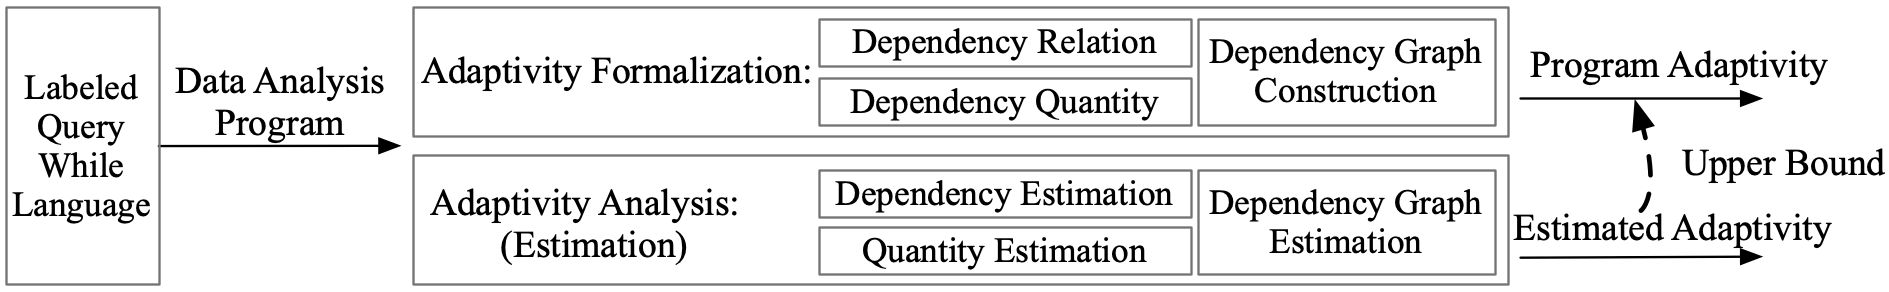
\includegraphics[width=1.0\textwidth]{architecture.png}
%     \vspace{-0.8cm}
%   \caption{High level architecture}
%     \label{fig:structure}
%     \vspace{-0.6cm}
% \end{figure}

\subsubsection{Static analysis}
%%%%%%%%%%%%%%%%%%%%%%%%%%%%%%% Previous Version Below that might be useful when make passes %%%%%%%%%%%%%%%%%
%  \detailed{The definition of adaptivity comes from the aforementioned execution-based dependency graph, 
%  our static analysis statically provides a sound upper bound on this adaptivity, via constructing another weighted graph, we call it estimated dependency graph. The upper bound is then found by searching a sound path with respect to our adaptivity in the generated graph. Different from the execution-based dependency which needs the trace from the execution, estimated one is built by our static analysis algorithm which takes the program itself as input. In brief, our algorithm is consist of a graph-generation algorithm, a weight computation algorithm and finally a path searching algorithm in the generated weighted graph.
%  }
%%%%%%%%%%%%%%%%%%%%%%%%%%%%%%% Previous Version Below that might be useful when make passes %%%%%%%%%%%%%%%%%
% \todo{In order to have a sound and accurate upper bound on the  adaptivity of a program $c$,
% we design a program analysis framework named {\THESYSTEM}.
% This framework composes two algorithms as shown in the double-stroke box and the dashed box in Fig.~\ref{fig:adaptfun}.
% The first algorithm in the double-stroke box combines the quantitative and dependency analysis techniques.
% It produces an estimated \emph{dependency graph} for a program.
% The second algorithm in the dashed box is a walk length estimation algorithm.
% It computes the upper bound on the program's \emph{adaptivity} over the estimated graph.}
% \jl{Since the definition of adaptivity comes from the aforementioned execution-based dependency graph, 
%  our static analysis statically provides a sound upper bound on this adaptivity via approximating this graph. The estimated graph is called \emph{estimated dependency graph}. 
%  The upper bound is then computed by searching the walk in this graph such that it can give a sound bound on the adaptivity.
%  Different from the execution-based dependency graph, the estimated one is produced by our static anlaysis algorithm, which only takes the program as input and does not rely on the execution history.
%  In brief, our algorithm is consist of a weighted graph-generation algorithm and a adaptivity computation algorithm over the graph.
%  }
 
 %%%%%%%%%%%%%%%%%%%%%%%%%%%%%%% Previous Version Above for Reference  %%%%%%%%%%%%%%%%%
To compute statically a sound and accurate upper bound on the \emph{adaptivity} of a program $c$,
we design a program analysis framework named {\THESYSTEM} which we will describe formally in Section \ref{sec:algorithm}. 
The structure of {\THESYSTEM} (Fig.~\ref{fig:adaptfun}) reflects in part the definition of adaptivity we discussed in the previous section. Specifically, {\THESYSTEM} is composed by two algorithms (the ones in dashed boxes in the figure), one for building a dependency graph, which we call \emph{estimated dependency graph}, and the other to estimate the adaptivity from this graph.  
The first algorithm generates the \emph{estimated dependency graph} using several program analysis techniques. Specifically,
 {\THESYSTEM} extracts the vertices and the query annotations by looking at the assigned variables of the program, it estimates the edges by using control flow and data flow analysis, and it estimates the weights by using symbolic reachability-bound analysis---weights in this graph are symbolic expressions over input variables. 
% This combined analysis allow us to obtain more accurate upper bounds than what we would obtain by using any of these single analysis technique in isolation.
The second algorithm estimates the
% longest 
walk which respects the weights and which visits the maximal number of query vertices.
%  as possible. 
The two algorithms together gives us an  upper bound on the program's \emph{adaptivity}.

 \begin{figure}
  \centering    
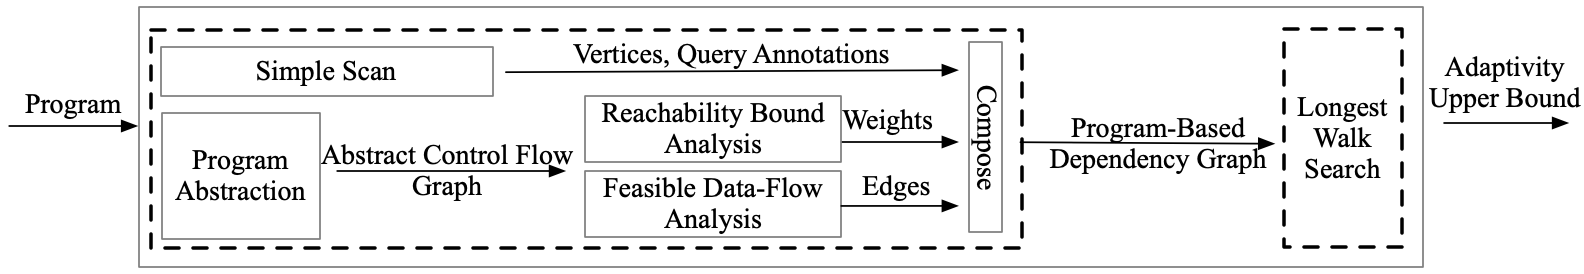
\includegraphics[width=1.0\columnwidth]{adapfun.png}
  \vspace{-0.8cm}
  \caption{The overview of {\THESYSTEM}}
  \label{fig:adaptfun}
  \vspace{-0.5cm}
\end{figure}

 
%%%%%%%%%%%%%%%%%%%%%%%%%%%%%%%%%%% Details Below that might be useful when others are making passes %%%%%%%%%%%%%%%%%
%   \detailed{Fig.~\ref{fig:overview-example}(c) is the resulting estimated graph of our static analysis algorithm which consumes the program in Fig.~\ref{fig:overview-example}(a).The edges are generated by our graph generation algorithm which combines control flow analysis and data flow analysis, presented in Section~\ref{sec:alg_edgegen}). We can easily see the generated graph in Fig.~\ref{fig:overview-example}(c) is a safe approximation of its execution-based counterpart in Fig.~\ref{fig:overview-example}(b), in the way that we can find a corresponding edge in Fig.~\ref{fig:overview-example}(c) for all the edges in Fig.~\ref{fig:overview-example}(b). We call the weight of every vertex computed by our algorithm as estimated weight,  }
%   estimated by using a reachability-bound estimation algorithm (presented in Section~\ref{sec:alg_weightgen}). \detailed{Different from the execution-based weight $w_1$ or $w_k$ in Fig.~\ref{fig:overview-example}(b) which is a function whose output relies on the initial trace, our estimated weight} can be symbolic and provide a sound upper bound on its execution-based weight of the corresponding vertex in the execution-based dependency graph. For instance, 
%   the estimated weight $k$ of the vertex $x^{3}$ in Fig.~\ref{fig:overview-example}(c) is a sound upper bound on the execution-based weight $w_k$ of vertex $x^{3}$ in Fig.~\ref{fig:overview-example}(b), with the same starting trace $\trace$, $w_k(\trace) \leq\trace(k)$. $\trace(k)$ means getting the value of variable $k$ in the trace $\trace$. The soundness of this step is proved in Theorem~\ref{thm:addweight_soundness}.   
%
We show in Fig.~\ref{fig:overview-example}(c) the estimated dependency graph that our static analysis algorithm returns for the program $\kw{twoRounds(k)}$ in Fig.~\ref{fig:overview-example}(a).
Vertices and query annotations are the same as the ones in Fig.~\ref{fig:overview-example}(b) and they are simply inferred by scanning the program.
As we said before, the edges are estimated using control flow and data flow analysis.
For the $\kw{twoRounds(k)}$ example, every edge in Fig.~\ref{fig:overview-example}(b) is precisely inferred by our combined analysis, this is why Fig.~\ref{fig:overview-example}(c) contains exactly the same edges.
The weight of every vertex is computed using a reachability-bound estimation algorithm which outputs a symbolic expression over the input variables, in the example only $k$, representing an upper bound on the number of times each assignment is executed.
% \wq{symbolic and provide a sound upper bound on its execution-based weight of the corresponding vertex in the execution-based dependency graph.
% $w_k(\trace) \leq \trace(k)$. $\trace(k)$ means getting the value of variable $k$ in the trace $\trace$. The soundness of this step is proved in Theorem~\ref{thm:addweight_soundness}.}
For example, consider the vertex $x^{3}$, its weight is $k$ and this provides an upper bound on the value returned by the weight function $\lambda \trace. \rho(\trace)k$ associated with vertex $x^{3}$ in Fig.~\ref{fig:overview-example}(b) for any initial state. 
% Indeed, 
% for any initial trace $\trace_0$, when $w_{x^{3}}(\trace_0)$ executes the program and counts the
% execution times of command $3$,
% we expect that this counts is at most the the loop iterations, i.e. $k$'s initial value from $\trace_0$.

The algorithm searching for the walk first finds a path $l^6:{}^1_1 \to a^5: {}^k_0 \to x^3: {}^k_1$, and then constructs a walk based on this path. Every vertex on this walk is visited once, and the number of vertices with query annotation $1$ in this walk is $2$, which is the upper bound we expect.
{It is worth noting here that $x^3$ and $a^5$ can only be visited once because there isn't an edge to go back to them, even though they both have the weight $k$}.
In this sense, instead of simply computing the weighted length of this path ($2k+1$) as adaptivity, the algorithm $\pathsearch$ computes the upper bound $2$. Note that $2$ is not always tight, for example when $k = 0$.
% \todo{Can you double check if this is clear?}
% \mg{I think we should add a sentence to say that this bound is actually not always tight.}

%%%%%%%%%%%%%%%%%%%%%%%%%%%%%%%%%%%%%%%%%%% Language %%%%%%%%%%%%%%%%%%%%%%%%%%%%%%%%%%%%%%%%%%%
\section{Labeled Query  While  language }
\label{sec:loop_language}
{The language of {\THESYSTEM} is a standard while language with labels to identify different components and with primitives for queries, and equipped with a  trace-based operational semantics which is the main technical tool we will use to define the program's adaptivity.

%\subsection{Syntax}
%\label{sec:syntax}
\vspace{-0.1cm}
{\small
\[
\begin{array}{llll}
\mbox{Arithmetic Expression} 
& \aexpr & ::= & 
n ~|~ {x} ~|~ \aexpr \oplus_a \aexpr 
~|~ \elog \aexpr  ~|~ \esign \aexpr ~|~ \max(a, a) ~|~ \min(a, a)
\\
\mbox{Boolean Expression} & \bexpr & ::= & 
%
\etrue ~|~ \efalse  ~|~ \neg \bexpr
 ~|~ \bexpr \oplus_b \bexpr
%
~|~ \aexpr \sim \aexpr 
\\
%
\mbox{Expression} & \expr & ::= & v ~|~ \aexpr \sep \bexpr ~|~ [\expr, \dots, \expr]
\\  
%
\mbox{Value} 
& v & ::= & { n \sep \etrue \sep \efalse ~|~ [] ~|~ [v, \dots, v]}  
\\
%
\mbox{Query Expression} 
& {\qexpr} & ::= 
& { \qval ~|~ \aexpr ~|~ \qexpr \oplus_a \qexpr ~|~ \chi[\aexpr]} 
\\
%
\mbox{Query Value} & \qval & ::= 
& {n ~|~ \chi[n] ~|~ \qval \oplus_a  \qval ~|~ n \oplus_a  \chi[n]
    ~|~ \chi[n] \oplus_a  n}\\
\mbox{Label} 
& l & \in & \mathbb{N} \cup \{\lin, \lex\} \\
\mbox{Labeled Command} 
& {c} & ::= &   [\assign {{x}}{ {\expr}}]^{l} ~|~  [\assign {{x} } {{\query(\qexpr)}}]^{l}
~|~ {\ewhile [ \bexpr ]^{l} \edo {c} }
 \\
 &&&
~|~ {c};{c}  
~|~ \eif([\bexpr]{}^l , {c}, {c}) 
~|~ [\eskip]^l 
\end{array}
\]
\vspace{-0.1cm}
}

%%%%%%%%%%%%%%%%%%%%%%%%%%%%%%%%%%% Details on Explaining the Syntax and Operational Semantics,
%%%%%%%%%%%%%%%%%%%%%%%%%%%%%%%%%%% that might be useful when others are making passes %%%%%%%%%%%%%%%%%
% \wq{As we have seen in the $\kw{twoRounds(k)}$ example in Fig.~\ref{fig:overview-example}(a), a program is expressed by labeled commands $c$. Our language supports the composition of labeled commands $c;c$, $[skip]^l$, the if condition $\eif([\bexpr]^l, c, c)$, the while command $\ewhile [\bexpr]^l \edo {c} $. The label $l$ records the location of this command, as a nature number $\mathbb{N}$ indicating the line number. Besides, it can also be $in$ or $ex$, used for annotating input variables and results and will not show up in labeled commands.} \wqside{Is it true that in and ex will not appear in the l in command?} 
%
% The boolean condition $b$ of the if and while commands is a standard boolean expression, which covers {\tt true} or {\tt false}, basic boolean connectives such as logical and logical or denoted by $\oplus_b$, logical negation $\neg$, and also comparison between arithmetic expressions $a \sim a$,  where $\sim$ stands for the basic operations such as $\leq,=,<,$ etc.  The arithmetic expression $a$ can be a constant $n$ denoting integer, a variable $x$ from some countable variable set $\mathcal{VAR}$, binary operation $\oplus_a$ such as addition, product, subtraction, etc, over arithmetic expressions, log and sign operation, minimal and maximum of two arithmetic expressions. An expression $e$ is then either a standard arithmetic expression or a boolean expression, or a list of expressions.
%
% \wq{As a reminder, the vertices of either the execution-based or program-based graphs in Fig.~\ref{fig:overview-example}(b) or Fig.~\ref{fig:overview-example}(c) are assigned variables and these assigned variables come from our two assignment commands: the standard assignment $[\assign{x}{\expr}]^l$, and our main novelty, the query request assignment $[\assign{x}{q(\qexpr)}]^l$.  The query is specified by a query expression $\qexpr$, which contains the necessary information for a query request. The query expression can be either the normal form $\alpha$, or just an arithmetic expression $a$ to express constant queries, or $\chi[\aexpr]$ representing the values at a certain index $\aexpr$ in a row $\chi$ of the database. Besides, we also allow combined access to the database in query expressions by means of $\qexpr \oplus \qexpr$.} For example, $\chi[3] + 5$ represents a query which asks the value from the column 3 of each database raw $\chi$, adds 5 to each of these values, and then computes the average of these values.
% In reality, if a data analyst wants to ask a simple linear query which returns the first element of the row, they can simply use the command $ \assign{x}{q(\chi[1])}$ in their data analysis program.
Expressions include
standard arithmetic (with value $n \in \mathbb{N}\cup \{ \infty \}$) and boolean expression, ($\aexpr$ and $\bexpr$) and extended query expressions $\qexpr$.
A query expression $\qexpr$ can be either a simple arithmetic expression $a$, an expression of the form $\chi[\aexpr]$ where $\chi$ represents a row of the database  and  $\aexpr$ represents an index used to identify a specific attribute of the row $\chi$, a combination of two query expressions, $\qexpr \oplus_{a} \qexpr$, or a normal form $\qval$.
For example, the query expression $\chi[3] + 5$  denotes the computation that
obtains
the value in the $3$rd column of $\chi$ in one row and then adds $5$ to it.

Commands are the typical ones from while languages with an additional command $\assign{x}{\query(\qexpr)}$ for query requests which can be used to interrogate
 the database and compute the linear query corresponding to $\qexpr$.
Each command is annotated with a label $l$, and we will use natural numbers as labels to record
the location of each command, so that we can uniquely identify them.
We also have a set of labels $\ldom$, a set $\mathcal{LV}$  of labeled variables (simply variables with a label), and a set $\cdom$ of all the programs.
We denote by $\mathbb{LV}(c)$ the set of labeled variables assigned in an assignment command in the program $c$.  
We denote by  $\qvar(c)$ the set of labeled variables that are assigned the result of a query in the program $c$.
 \highlight{We provide the table of notations in Table~\ref{tb:notation} for quick reference.}

% \mg{Please double check this notation.}


% In this the command, the query expression $\qexpr$ is sent to the database server as a request.
% Then the server will compute the average value of $\qexpr$ over each row of the hidden database $\chi$ and return us the result.
% For instance, when we execute the command $\assign{x}{\query(\chi[3] + 5)}$,
% the server will receive query request in form of $\chi[3] + 5$,
% then compute the average value of $\chi[3] + 5$ over each raw of $\chi$, and return the result to us. 
% The server is used as external API for computing the results over the hidden database $\chi$.

\subsection{ Trace-based Operational Semantics}

%  \wq{Our operational semantics uses the trace $\trace \in \mathcal{T}$ to track the history of the program execution, we use $\mathcal{T} $ for the set of traces. To be precise, the trace is a list of events and an event tracks the useful information about one step of the evaluation. When a program $c$ is evaluated in our operational semantics$\config{c, \trace} \to \config{c', \trace'} $, it starts with an initial trace $\trace$, evaluates to $c'$ , and along with the program evaluation, events are collected in the evaluation order and appended to $\trace$, and then we get the result trace $\trace'$. We can easily get the history of the evaluation of the program $c$ by looking at these newly added events in $\trace$ with respect to the initial trace $\trace$.  }
% \highlight{Comment: A lot of notation is provided in section 3.1, some standard and some less-so. A table to summarize would be helpful for the reader to orient themselves during the rest of the paper. On a minor note: the combine operator (::) is used only once (in figure 5) which the concat operator (++) is used everywhere else (e.g., definitions 2 and 4) with singleton traces.}
We use a trace-based operational semantics tracking the history of program execution. The operational semantics is parameterized by a database that can be accessed only through queries. Since this database is fixed, we omit it from the semantics but it is important to keep in mind that this database exists and it is what allows us to evaluate queries.
A \emph{trace}
$\trace$ is a list of \emph{events} generated when executing specific commands. We denote by $\mathcal{T}$ the set of traces and we will use list notation for traces,
 where $[]$ is the empty trace, the operator $\traceadd$ combines an event and a trace in a new trace, 
and the operator $\tracecat$ concatenates two traces. 
We have two kinds of events: \emph{assignment events} and \emph{testing events}. 
Each event consists of a quadruple,
and we use $\eventset^{\asn}$ and $\eventset^{\test}$ to denote the set of all assignment events and testing events, respectively.
% \begin{center}
% $ \begin{array}{lllll}
% \mbox{Event} 
% & \event & ::= & 
% {({x}, l, v, \bullet)} ~|~ { ({x}, l, v, \qval)}  ~|~{(\bexpr, l, v, \bullet)}  
% \\
% \end{array}$
% \end{center}
\begin{center}
  $ \begin{array}{lllll}
  \mbox{Event} 
  & \event & ::= & 
  ({x}, l, v, \bullet) ~|~ ({x}, l, v, \qval)  & \mbox{Assignment Event} \\
  &&& ~|~(\bexpr, l, v, \bullet)  & \mbox{Testing Event}
  \\
  \end{array}$
  \end{center}
An assignment event tracks the execution of an assignment  or a query request and consists of the assigned variable, the label of the command that generates it, the value assigned to the variable, and the normal form  $\qval$ of the query expression that has been requested, if this command is a query request, otherwise a default value $\bullet$.
A testing event tracks the execution of an if or while command and consists of the guard of the command, the label, the result of evaluating the guard, the last element $\bullet$. 
 We use the operator $\env (\trace) x$ to fetch the latest value assigned to  $x$ in the trace $\trace$, the operator
$\vcounter$ to count the occurrence of a labeled variable in the trace. \highlight{ The function $\kw{lastVal}(\tau, x)$ mentioned in Section~\ref{sec:adaptivity-informal} can be 
expressed as $\lambda \trace. \env (\trace) x$. For any initial trace $\trace$, $\kw{lastVal}(\tau, x)$ returns the latest value of $x$ in $\trace$.
}
We denote by $\tlabel(\trace) \subseteq \ldom$ the set of the labels occurring in $\trace$.
Finally, we use $\mathcal{T}_0(c) \subseteq \mathcal{T}$ to denote the set of \emph{initial traces}, the ones
which assign a value to the input variables. We use $\eventset$ to denote the set of all events.


The trace-based operational semantics is described in terms of a small step evaluation relation
$\config{c, \trace} \to \config{c', \trace}'$  describing how a configuration program-trace evaluates to another
configuration program-state. Selected rules are shown in Fig.~\ref{fig:os}.
The rules for assignment and query generate assignment events, while the rules for while and if generate testing events. 
We have relations $\config{\trace, \expr} \earrow v $  and $\config{\trace, \bexpr} \barrow v $  to evaluate expressions and boolean expressions, respectively. 
%   \mg{Can you please confirm that this is true?} Yes
The only rule that is non-standard is the $\textbf{query}$ rule. When evaluating a query, the query expression $\qexpr$ is first simplified to its normal form $\alpha$ using an evaluation relation $\config{\trace, \qexpr} \qarrow \qval$. 
The normal form $\qval$ characterizes the linear query that is run against the database. The query result $v$ is the expected value of the function $\lambda \chi.\qval$ applied to each row of the dataset. We summarize this process with the notation $\query(\qval) = v$ in the rule $\textbf{query}$. 
Once the answer of the query is computed, the rules record all the needed information in the trace.  We will use $\to^*$ for the reflexive and transitive closure of $\to$. 
%%%%%%%%%%%%%%%%%%%%%%%%%%%%%%%%%%% The Detailed Version in Explaining the Event %%%%%%%%%%%%%%%%%%%%%%%%%%%%%%%%%%%%%%%%%%%%%%%%%
% First of all, as the key component of the program evaluation history, an event $\event$ stores necessary information on the evaluation results of commands. Depending on the types of commands, there are two kinds of events: the assignment event which is generated in the standard assignment and query request assignment commands, and the testing event which is generated in an if or while command. Both assignment and testing events are quadruples, but store different contents. 
%\jl{
% The key component of the program evaluation history is the event $\event$,
% which stores necessary information on the evaluation results of commands.
%%%%%%%%%%%%%%%%%%%%%%%%%%%%%%%%%%% The Detailed Version in Explaining the Assignment evaluation %%%%%%%%%%%%%%%%%%%%%%%%%%%%%%%%%%%%%%%%%%%%%%%%%
% The assignment event 
% targets the assignment so it needs to maintain the mapping between labeled assigning variable and the result assigned, to this end, the first three elements of the quadruple of an assignment event are the variable, the label, and the result $v$ of the assigned expression. Look at the rule $\textbf{assn}$ and rule $\textbf{query}$ in Fig.~\ref{fig:os}, the result $v$ is different: in the standard assignment, $v$ is the evaluation result of the assigned expression $e$ by the standard expression evaluation $\config{\trace, \expr} \earrow v $; in the query request assignment, the query expression $\qexpr$ is evaluated to its normal form $\alpha$ by the query expression evaluation $\config{\trace, \qexpr} 
% \qarrow \qval$ and is sent to a hidden mechanism, $query(\alpha) = v$ means that the return result of this query represented by $\alpha$ from the mechanism is $v$. Another difference of the generated assignment events in these two rules lands in the last element of the quadruple, which stores the query information. In the rule $\textbf{query}$, the fourth element is the query normal form $\alpha$ which is sent to the mechanism, while in the standard assignment rule $\textbf{assn}$, we use $\bullet$ to show this event is not directly related to a query request.
% \jl{The assignment event is generated when evaluating an assignment command or query request. It stores the value assigned to each variable and tracks the query request.
% The first three elements are the variable, the label of this command, and the value assigned to this variable.
% The forth element is the normal form of a query expression, $\qval$ if this command is a query request, otherwise a default value $\bullet$.
% As in rule $\textbf{assn}$ and rule $\textbf{query}$ in Fig.~\ref{fig:os}.
% When evaluating a query request, the query expression $\qexpr$ is first simplified to its normal form $\alpha$ by the evaluation rule $\config{\trace, \qexpr} \qarrow \qval$. 
% Then $\qval$ is sent to the hidden database on unknown server, which computes the query result and send back to us.
% This computation process is simplified into $\query(\qval) = v$ in the rule $\textbf{query}$.
% }
%%%%%%%%%%%%%%%%%%%%%%%%%%%%%%%%%%% The Detailed Version in Explaining the Expression Evaluation %%%%%%%%%%%%%%%%%%%%%%%%%%%%%%%%%%%%%%%%%%%%%%%%%
% \detailed{
% The expression evaluation $\config{\trace, \expr} \earrow v $ relies on the evaluation of arithmetic expressions $\config{\trace,\aexpr} \aarrow v $ and boolean expressions $\config{\trace, \bexpr} \barrow v $, they are standard and we leave The full rules in the appendix. The evaluation rules of query expressions are presented below.}
The query expression evaluation relation  $\config{\trace, \qexpr} \qarrow \qval$ is defined by the following rules which reduce a query expression to its normal form.
{\small
\begin{mathpar}
\inferrule{ 
  \config{\trace, \aexpr} \aarrow n
}{
 \config{\trace,  \aexpr} 
 \qarrow n
}
\and
\inferrule{ 
  \config{\trace, \qexpr_1} \qarrow \qval_1
  \and
  \config{\trace, \qexpr_2} \qarrow \qval_2
}{
 \config{\trace,  \qexpr_1 \oplus_a \qexpr_2} 
 \qarrow \qval_1 \oplus_a \qval_2
}
\and
\inferrule{ 
  \config{\trace, \aexpr} \aarrow n
}{
 \config{\trace, \chi[\aexpr]} \qarrow \chi[n]
}
\and
\inferrule{ 
  \empty
}{
 \config{\trace,  \qval} 
 \qarrow \qval
}
 \end{mathpar}
 }
%%%%%%%%%%%%%%%%%%%%%%%%%%%%%%%%%%% The Detailed Version in Explaining the Testing Event %%%%%%%%%%%%%%%%%%%%%%%%%%%%%%%%%%%%%%%%%%%%%%%%%
% The testing event is generated when evaluating if and while commands. To record the control flow information, the first element of the event is the guard $b$ in both if and while rules $\textbf{if-t,if-f}$ and rule $\textbf{while-t, while-f}$. The third element then stores the evaluation results of this guard, either true or false. Since the guard can not be a query request, the last element is $\bullet$. 
%%%%%%%%%%%%%%%%%%%%%%%%%%%%%%%%%%% The Details for The If and While Evaluation %%%%%%%%%%%%%%%%%%%%%%%%%%%%%%%%%%%%%%%%%%%%%%%%%
% \detailed{The rules for if hand while both have two versions, when the guard evaluates to true and false, respectively. In these rules, the evaluation of the guard also generates testing event and our trace is updated as well. }
% The rules for if and while both have two versions, 
% when the boolean expressions in the guards are evaluated to true and false, respectively. 
% In these rules, the evaluation of the guard generates a testing event and the trace is updated as well by appending this event.
% The rule $\textbf{query}$ evaluates the argument of a query request to a normal form and obtain the answer $v_q$ of the query $\query(v)$ from the mechanism. 
% Then the trace expanded by appending the query expression $\query(v)$ with the current annotation $(l,w)$. 
% The rule for assignment is standard and the trace remains unchanged. The sequence rule keeps tracking the modification of the trace, and the evaluation rule for if conditional 

%By the operational semantics rules, we prove no rule will shrink the trace in Appendix.
{\footnotesize %
\begin{figure}
\begin{mathpar}
\boxed{
\mbox{Command $\times$ Trace}
\xrightarrow{}
\mbox{Command $\times$ Trace}
}
\and
\boxed{\config{{c, \trace}}
\xrightarrow{} 
\config{{c',  \trace'}}
}
\\
\inferrule
{
\config{\trace, \expr} \earrow v 
\and
\event = ({x}, l, v, \bullet)
}
{
\config{[\assign{{x}}{\expr}]^{l},  \trace } 
\xrightarrow{} 
\config{\clabel{\eskip}^l, \trace \traceadd \event}
}
~\textbf{assn}
%
\and

{
\inferrule
{
 \trace, \qexpr \qarrow \qval
 \and 
\query(\qval) = v
\and 
\event = ({x}, l, v, \qval)
}
{
\config{{[\assign{x}{\query(\qexpr)}]^l, \trace}}
\xrightarrow{} 
\config{{\clabel{\eskip}^l,  \trace \traceadd \event} }
}
~\textbf{query}
}
%
\and
%
\inferrule
{
 \trace, b \barrow \etrue
 \and 
 \event = (b, l, \etrue, \bullet)
}
{
\config{{\ewhile [b]^{l} \edo c, \trace}}
\xrightarrow{} 
\config{{
c; \ewhile [b]^{l} \edo c,
\trace \traceadd \event}}
}
~\textbf{while-t}
%
%
% \quad
% %
% \inferrule
% {
%  \trace, b \barrow \efalse
%  \and 
%  \event = (b, l, \efalse, \bullet)
% }
% {
% \config{{\ewhile [b]^{l}, \edo c, \trace}}
% \xrightarrow{} 
% \config{{
%   \clabel{\eskip}^l,
% \trace \traceadd \event}}
% }
% ~\textbf{while-f}
% %
% %
% \and
% \inferrule
% {
% \config{{c_1, \trace}}
% \xrightarrow{}
% \config{{c_1',  \trace'}}
% }
% {
% \config{{c_1; c_2, \trace}} 
% \xrightarrow{} 
% \config{{c_1'; c_2, \trace'}}
% }
% ~\textbf{seq1}
% \and
% \inferrule
% {
%   \config{{c_2, \trace}}
%   \xrightarrow{}
%   \config{{c_2',  \trace'}}
% }
% {
% \config{{\clabel{\eskip}^l; c_2, \trace}} \xrightarrow{} \config{{ c_2', \trace'}}
% }
% ~\textbf{seq2}
% \quad
% \inferrule
% {
%  \trace, b \barrow \etrue \and \event = (b, l, \etrue, \bullet)
% }
% {
%  \config{{
% \eif([b]^{l}, c_1, c_2), 
% \trace}}
% \xrightarrow{} 
% \config{{c_1, \trace \traceadd \event}}
% }
% ~\textbf{if-t}
% \and
% %
% \inferrule
% {
%  \trace, b \barrow \efalse
%  \and 
%  \event = (b, l, \efalse, \bullet)
% }
% {
% \config{{\eif([b]^{l}, c_1, c_2), \trace}}
% \xrightarrow{} 
% \config{{c_2, \trace \traceadd \event}}
% }
% ~\textbf{if-f}
\end{mathpar}
  \vspace{-0.5cm}
    \caption{Trace-based Operational Semantics for Language.}
    \label{fig:os}
  \vspace{-0.1cm}
\end{figure}
}

    \begin{table}
      \caption{\highlight{Table of Notations}}
      \label{tb:notation}
      \begin{center}
        \begin{tabular}{| c |c |c| c| }
          \hline 
          $\mathcal{LV}$   & universe of labeled variables  & $\qvar(c)$ & labeled query variables in $c$\\ 
          $\cdom$  & set of all programs &  $\trace$ &   trace, a list of \emph{events}\\  
          $\mathcal{T}$  &  set of traces &  $\trace \traceadd \event$  & combine a trace and an event  \\
          $\ldom$ & set of labels  & $\trace \tracecat \trace'$ &  trace concatenation \\
          $\tlabel(\trace) $  &set of labels occurring in $\trace$  &  $ \env (\trace) x$  & fetch latest value of  $x$ in a given $\trace$ \\
          $\mathcal{T}_0(c) $ &  set of \emph{initial traces} & $\kw{lastVal} (\trace, x)$  & fetch latest value of  $x$ in any $\trace$\\
          $\mathbb{LV}(c)$  & labeled variables in $c$ & $\vcounter(\trace, x^i)$ & occurrence of $x^i$ in the trace $\trace$\\
          \hline 
        \end{tabular}
        \end{center}
        \vspace{-0.3cm}
      \end{table}
}
%%%%%%%%%%%%%%%%%%%%%%%%%%%%%%%%%%%%%%%%%%% Adaptivity %%%%%%%%%%%%%%%%%%%%%%%%%%%%%%%%%%%%%%%%%%% 
\section{Definition of Adaptivity}
\label{sec:adaptivity}
In this section, we formally present the definition of adaptivity of a program, which is the length of the 'longest' walk with most queries involved in the semantics-based dependency graph of this program. We first present the construction of the semantics-based dependency graph before the introduction of the formal definition of adaptivity. 

\subsection{Semantics-based Dependency Graph}
\label{sec:design_choice}
%%%%%%%%%%%%%%%%%%%%%%%%%%%%%%%%%%% The Detailed Version in Introducing The Dependency Graph %%%%%%%%%%%%%%%%%%%%%%%%%%%%%%%%%%%%%%%%%%%%%%%%%
% we formally define the semantics-based dependency graph as follows. There are some notations used in the definition. The labeled variables of a program $c$  
% is a subset of the labeled  variables $\mathcal{LV}$, denoted by $\lvar(c) \in \mathcal{P}(\mathcal{VAR} \times \mathcal{L}) \subseteq \mathcal{LV}$.
% \wq{I think LV(c) means all the labeled assigned variables, because in Fig.3.b, j2 is not in the graph so j2 is not in LV(tworounds), please verify. If so, maybe LV(c) is not a good name, people may think it means all the label variables, instead of just assigned ones.}
% The set of query-associated variables (in query request assignments) for a program $c$ is denoted as $\qvar(c)$, where $\qvar: \cdom \to 
% \mathcal{P}(\mathcal{LV})$. The set of initial traces of a program $c$ is a subset of the  trace universe $\trace$, in which every initial trace contains the value for all the input variables of $c$. For instance, the initial trace $\trace_0$ contains the value of input variable $k$ in the $\kw{twoRounds(k)}$ example.
\jl{
The \emph{semantics-based dependency graph} is formally defined in Definition~\ref{def:trace_graph}. 
For a program $c$, there are some notations used in the definition.
The labeled variables of $c$,
$\lvar(c) \subseteq \mathcal{LV}$ contains all the variables in $c$'s assignment commands, with the command labels as superscripts. 
The set of query-associated variables (in query request assignments),
$\qvar(c) \subseteq \lvar(c)$ contains all labeled variables in $c$'s query requests. 
The set of initial traces of $c$,
$\mathcal{T}_0(c) \subseteq \mathcal{T}$
contains all possible initial trace of $c$.
Each initial trace,  $\trace_0 \in \mathcal{T}_0(c)$ contains the initial values of all input variables of $c$. 
For instance, the initial trace of $\kw{twoRounds(k)}$ example contains the initial value of the input variable $k$.
}
\begin{defn}[Semantics-based Dependency Graph]
\label{def:trace_graph}
Given a program ${c}$,
its \emph{semantics-based dependency graph} 
$\traceG({c}) = (\traceV({c}), \traceE({c}), \traceW({c}), \traceF({c}))$ is defined as follows,
{\small
\[
\begin{array}{lll}
  \text{Vertices} &
  \traceV({c}) & := \left\{ 
  x^l
  ~ \middle\vert ~ x^l \in \lvar(c)
  \right\}
  \\
  \text{Directed Edges} &
  \traceE({c}) & := 
  \left\{ 
  (x^i, y^j) 
  ~ \middle\vert ~
  x^i, y^j \in \lvar(c) \land \vardep(x^i, y^j, c) 
  \right\}
  \\
  \text{Weights} &
  \traceW({c}) & := 
  \{ 
  (x^l, w) 
  ~ \vert ~ 
  w : \mathcal{T}_0(c) \to \mathbb{N}
  \land
  x^l \in \lvar(c) 
  \\ & &
  \quad \land
  \forall \trace_0 \in \mathcal{T}_0(c), \trace' \in \mathcal{T} \st \config{{c}, \trace_0} \to^{*} \config{\eskip, \trace_0\tracecat\trace'} 
  \implies w(\trace_0) = \vcounter(\trace', l) \}
  \\
  \text{Query Annotations} &
  \traceF({c}) & := 
\left\{(x^l, n)  
~ \middle\vert ~
 x^l \in \lvar(c) \land
n = 1 \Leftrightarrow x^l \in \qvar(c) \land n = 0 \Leftrightarrow  x^l \notin \qvar(c)
\right\}
\end{array},
\]
}
%%%%%%%%%%%%%%%%%%%%%%%%%%%%%%%%%%% The Detailed Version in Explaining the Trace Operators %%%%%%%%%%%%%%%%%%%%%%%%%%%%%%%%%%%%%%%%%%%%%%%%%
% There are some operators: the trace concatenation operator $\tracecat: \mathcal{T} \to \mathcal{T} \to \mathcal{T}$, combines two traces; the counting operator $\vcounter : \mathcal{T} \to \mathbb{N} \to \mathbb{N}$, 
% which counts the occurrence of of a labeled variable in the trace. The full definitions of these above operators can be found in the appendix.
% \\
\jl{where $\tracecat: \mathcal{T} \to \mathcal{T} \to \mathcal{T}$ is the trace concatenation operator, which combines two traces, 
and $\vcounter : \mathcal{T} \to \mathbb{N} \to \mathbb{N}$ is the counting operator, 
which counts the occurrence of of a labeled variable in the trace. All the definition details are in the appendix.}
\end{defn}


%%%%%%%%%%%%%%%%%%%%%%%%%%%%%%%%%%% The Explanation of Dependency Graph %%%%%%%%%%%%%%%%%%%%%%%%%%%%%%%%%%%%%%%%%%%%%%%%%
% \wq{ The occurrence time is computed by the counter operator $w(\trace) = \vcounter(\trace', l)$. As an instance, in the semantics-based dependency graph of $\kw{twoRounds}$ in Figure~\ref{fig:overview-example}(b), the weight of vertices in the while loop $w_k$ is a function which returns the value $n$ of variable $k$ in the starting trace $\tau$, and the commands in the loop are indeed executed $n$ times when starting with $\trace$.}
% Every vertex also has a query annotation, mapping each $x^l \in \traceV(c)$ to $0$ or $1$, 
% indicating whether the vertex comes from a query request assignment (1) or not (0) by checking if the labeled variable $x^l$ of the vertex is in $\qvar(c)$.
% One interesting point is that instead of building a graph whose vertices are just variables coming from query request assignments, we choose the combination of all the labeled assigned variables of the program and the query annotations. The reason is that the results of previous queries can be stored or used in variables
% which aren't associated to the query request,
% it is necessary to track the dependency between all the assigned variables of the program. 
% The main novelty is the combination of the quantitative and dependency information on the semantics-based dependency graph, which means this graph can tell both the dependency between queries and the times they depend on each other.
% The vertices $\traceV({c})$ of a program $c$ are the labeled assigned variables, which are statically collected. The weight function on every vertex $w : \mathcal{T} \to \mathbb{N}$
% mapping from a starting trace $\trace \in \mathcal{T}_0(c)$ to a natural number, tracks the occurrence times of this vertex in the newly generated trace $\trace'$ when the program $c$ is evaluated from the starting trace $\config{{c}, \trace} \to^{*} \config{\eskip, \trace\tracecat\trace'} $.
% One interesting point is that instead of building a graph whose vertices are just variables coming from query request assignments, we choose the combination of all the labeled assigned variables of the program and the query annotations. The reason is that the results of previous queries can be stored or used in variables
% % which aren't associated to the query request,
% it is necessary to track the dependency between all the assigned variables of the program. 
\jl{There are four components in this graph.
\begin{enumerate}
    \item The vertices $\traceV({c})$ of a program $c$ are all its labeled variables, $\lvar(c)$ which are statically collected.
    \item $\traceF(c)$ contains the \emph{query annotation} for 
    every vertex $x^l \in \traceV(c)$. It indicates whether $x^l$ comes from a query request (1) or not (0) by checking if the labeled variable $x^l$ of the vertex is in $\qvar(c)$.
    \item Edges in $\traceE(c)$ are build from the $\vardep(x^i, y^j, c)$ relation between two labeled variables.
    This is the key definition in order to formalized the intuitive \emph{may-dependency} relation between queries and the \emph{adaptivity}. We present this formalization detail in Section~\ref{sec:dep} below.
    \item 
    The weight function in $\traceW(c)$ for each vertex, $w : \mathcal{T} \to \mathbb{N}$
maps from a starting trace $\trace_0 \in \mathcal{T}_0(c)$ to a natural number.
For each vertex $x^l$, it tracks its visiting times (i.e., the evaluation times of the command with the label $l$) when the program $c$ is evaluated from the initial trace $\trace_0$ into $\eskip$, $\config{{c}, \trace_0} \to^{*} \config{\eskip, \trace_0\tracecat\trace'} $.
The visiting times is computed by the counter operator $\vcounter(\trace', l)$
by counting the occurrence of the label $l$ in $\trace'$.
As an instance, in the semantics-based dependency graph of $\kw{twoRounds}$ in Figure~\ref{fig:overview-example}(b), the weight, $w_k$ of the vertex $x^3$ is a function of type $\mathcal{T}_0(\kw{twoRound(k)}) \to \mathbb{N}$.
Given input $\trace_0$, we execute the program under $\trace_0$ as $\config{\kw{twoRound(k)}, \trace_0} \to^{*} \config{\eskip, \trace_0\tracecat\trace'} $. Then $w_k(\trace_0)$ outputs the occurrence time of the label $3$ in $\trace'$.
\end{enumerate}
The main novelty of  the semantics-based dependency graph is the combination of the quantitative and dependency information. 
It can tell both the dependency between queries via the directed edge, and the times they depend on each other via the weight.
}

\subsection{May-Dependency}
\label{sec:dep}
%%%%%%%%%%%%%%%%%%%%%%%%%%%%%%%%%%% The Detail Explanation of Variable May-Dependency and Motivation on How to define it %%%%%%%%%%%%%%%%%%%%%%%%%%%%%%%%%%%%%%%%%%%%%%%%%
% \wq{we think the query $\query(\chi[2])$ (assigned variable $y^3$) may depend on the query $\query(\chi[1]$ (assigned variable $x^1$). 
  %  but vulnerable to queries request protected by differential privacy mechanisms. In our loop language, a query $q(e)$ represents a query request to the database through a mechanism, which add random noise to protect the return results. In this setting, the results of one query will be randomized due to the noise attached by the mechanism which fails the first candidate because witnessing the results of one query can no longer tells whether the change of the results comes from another query or the change of noise of the differential privacy mechanism. For example, suppose we have a program $p$ which requests two simple queries $q_1()$ and $q_2()$ with no arguments as follows.
%   \[
%   c_1 =\assign{x}{\query(\chi[2])} ;\assign{y}{\query(\chi[3] + x)}.
%   \]
%  $ c = \assign{x}{\query(\chi[1])} ; \assign{y}{\query(\chi[2])}$,
%  and 
% Specifically, in the {\tt Query While} language, the query request is composed by two components: a symbol $\query$ representing a linear query type and 
% % an argument
% the query expression $\qexpr$ as an argument, 
% which represents the function specifying what the query asks. 
% From our perspective, $\query(\chi[1])$ is different from $\query(\chi[2]))$. Informally,  
%
% in this example: $c_1 = \assign{x}{\query(0)}; \assign{z}{\query(\chi[x])}$.
% This candidate definition works well 
% Nevertheless, the first definition fails to catch control dependency because it just monitors the changes to a query, but misses the appearance of the query when the answers of its previous queries change. For instance, it fails to handle $}
%       c_2 = \assign{x}{\query(\chi[1])} ; \eif( x > 2 , \assign{y}{\query(\chi[2])}, \eskip )
%   $, but the second definition can. However, it only considers the control dependency and misses the data dependency. This reminds us to define a \emph{may-dependency} relation between labeled variables by combining the two definitions to capture the two situations.
%  $ p = \assign{x}{\query(\chi[1])} ; \assign{y}{\query(\chi[2])}$. 
% This candidate definition works well with respect to data dependency. However, if fails to handle control dependency since it just monitors the changes to the answer of a query when the answer of previous queries returned change. The key point is that this query may also not be asked because of an analyst decision which depend on the answers of previous queries. An example of this situation is shown in program $p_1$ as follows.
% There are two possible situations that a query will be "affected" by previous queries' results,  
% either when the query expression directly uses the results of previous queries (data dependency), or when the control flow of the program with respect to a query (whether to ask this query or not) depends on the results of previous queries (control flow dependency). To this end, our assigned variable dependency definition has the following two cases.   
% {
% \begin{enumerate}
%     \item One variable may depend on a previous variable if and only if a change of the value assigned to the previous variable may also change the value assigned to the variable.
%     \item One variable may depend on a previous variable if and only if a change of the value assigned to the previous variable may also change the appearance of the assignment command to this variable 
%     % in\wq{during?} 
%     during execution.
% \end{enumerate}
% }
%
%  The first case captures the data dependency. 
% For instance, in a simple program $c_1 =[\assign{x}{\query(\chi[2])}]^1 ;[\assign{y}{\query(\chi[3] + x)}]^2$, we think $\query(\chi[3] + x)$ (variable $y^2$) may depend on the query $\query(\chi[2]))$ (variable $x^1$), because the equipped function of the former $\chi[3] + x$ may depend on the data stored in x assigned with the result of $\query(\chi[2]))$. From our perspective, $\query(\chi[1])$ is different from $\query(\chi[2]))$. The second case captures the control dependency, for instance, in the program $
%       c_2 = [\assign{x}{\query(\chi[1])}]^1 ; \eif( [x > 2]^2 , [\assign{y}{\query(\chi[2])}]^3, [\eskip]^4 )
%
This section formalizes the \emph{may-dependency} relation between queries and introduces the
\emph{variable may-dependency} definition.

\jl{There are two possible situations that a query will be ``influenced'' by previous queries' results,
where either the query request is changed when the results of previous queries are changed (data dependency),
or the  query request is disappeared when the results of previous queries are changed (control dependency). In this sense, our formal dependency definition considers both the two cases as follows,
\begin{enumerate}
    \item One query may depend on a previous query if and only if a change of the value returned
    to the previous query request may also change this query request.
    \item One query may depend on a previous query if and only if a change of the value returned
    to the previous query request may also change the appearance of this query quest.
\end{enumerate}
The first case captures the data dependency. 
For instance, in a simple program $c_1 =[\assign{x}{\query(\chi[2])}]^1 ;[\assign{y}{\query(\chi[3] + x)}]^2$, we think $\query(\chi[3] + x)$ (variable $y^2$) may depend on the query $\query(\chi[2]))$ (variable $x^1$), because the equipped function of the former $\chi[3] + x$ may depend on the data stored in x assigned with the result of $\query(\chi[2]))$. From our perspective, $\query(\chi[1])$ is different from $\query(\chi[2]))$.
\\
The second case captures the control dependency.
For instance, in the program
$c_2 = [\assign{x}{\query(\chi[1])}]^1 ; \eif( [x > 2]^2 , [\assign{y}{\query(\chi[2])}]^3, [\eskip]^4 )$, 
we think the query $\query(\chi[2])$ ( or the labeled variable $y^3$) may depend on the query $\query(\chi[1])$ (via the labeled variable $x^1$). }

\jl{ 
Since both of the two ``influences'' are passing through labeled variables, we choose to formally define the \emph{may-dependency}
relation over all labeled variables, and then recover the query requests from query-associated variables, $\qvar(c)$.
It relies on formal observation of the ``influence'' via events in Definition~\ref{def:diff} and the \emph{may-dependency} between events in Definition~\ref{def:event_dep}.
}
\begin{defn}[Events Different up to Value ($\diff$)]
\label{def:diff}
Two events $\event_1, \event_2 \in \eventset$ are  \emph{Different up to Value},
denoted as $\diff(\event_1, \event_2)$ if and only if:
\begin{subequations}
\begin{align}
& \pi_1(\event_1) = \pi_1(\event_2) 
  \land  
  \pi_2(\event_1) = \pi_2(\event_2) \\
& \land  
  \big(
   (\pi_3(\event_1) \neq \pi_3(\event_2)
  \land 
  \pi_{4}(\event_1) =_q \pi_{4}(\event_2) = \bullet )
  \lor 
  (\pi_4(\event_1) \neq \bullet
  \land 
  \pi_4(\event_2) \neq \bullet
  \land 
  \pi_{4}(\event_1) \neq_q \pi_{4}(\event_2)) 
  \big)
\end{align}
\label{eq:diff}
\end{subequations}
where the projection operators $\pi_1,\pi_2,\pi_3$ and $\pi_4$ project the corresponding element from the quadruple of an event.
\end{defn}
%%%%%%%%%%%%%%%%%%%%%%%%%%%%%%%%%%% The "Detail" (I think redundant) Explanation of Variable May-Dependency and Motivation on How to define it %%%%%%%%%%%%%%%%%%%%%%%%%%%%%%%%%%%%%%%%%%%%%%%%%
% We use $\qexpr_1 =_{q} \qexpr_2$ and $\qexpr_1 \neq_{q} \qexpr_2$ to notate query expression equivalence and in-equivalence, distinct from standard equality. 
% First of all, $\diff(\event_1, \event_2)$ only compares the 'value' assigned to the same labeled variable so the two events share the same labeled variable (the first two elements of the event quadruple). If the labeled variable are not the same, it is trivially false. Next, the 'value' has different meaning according to the type of the assignment. If the two assignment events both are generated from a standard assignment command (by checking whether the fourth element of the event is $\bullet$), we think they are different up to their value if the value assigned to the variable (the third element of the event) varies. On the other hand, if they both come from query request assignment commands, we directly compare the query function (the fourth element of the event). We do not consider the case when one event is generated from the standard assignment and the other comes from the query request assignment, which will not hold. The motivation of defining  $\diff(\event_1, \event_2)$ is that it allows us to check whether the value assigned to a specific variable is changed or not in two runs, which is very important in our dependency case 1. 
\jl{
$\pi_1(\event_1) = \pi_1(\event_2) 
  \land  
  \pi_2(\event_1) = \pi_2(\event_2)$ at Eq.\ref{eq:diff}(a)
requires that $\event_1$ and $\event_2$ have the same variable name and label. 
This guarantees that $\event_1$ and $\event_2$ are generated from the same labeled command.
In Eq.\ref{eq:diff}(b),
two kinds of comparisons between the third and fourth element are for the non-query assignment and query request separately.
For events generated from the non-query assignments (via checking
$\pi_{4}(\event_1) =_q \pi_{4}(\event_2) = \bullet$), we only compare their assigned values through $\pi_3(\event_1) \neq \pi_3(\event_2)$.
But for these from query requests (via checking
$\pi_{4}(\event_1) \neq \bullet \land \pi_{4}(\event_2) \neq \bullet$),
we are comparing their query expressions by $\pi_{4}(\event_1) \neq_q \pi_{4}(\event_2)$ rather than the assigned value computed from the unknown database server.
This matches the intuitive data dependency between queries, where one query is influenced by others as long as the query request is changed.
}

\jl{Below is the \emph{event may-dependency} between events based on formally observing their differences via $\diff$.}
\begin{defn}[Event May-Dependency]
\label{def:event_dep}
An event $\event_2$ is in the \emph{event may-dependency} relation with an assignment event $\event_1 \in \eventset^{\asn}$ in a program ${c}$  with a hidden database $D$ and a witness trace $\trace \in \mathcal{T}$,
$\eventdep(\event_1, \event_2, [\event_1 ] \tracecat \trace \tracecat [\event_2], c, D)$ if and only if
\begin{subequations}
\begin{align}
&  
\exists \trace_0, \trace_1, \trace' \in \mathcal{T},\event_1' \in \eventset^{\asn}, {c}_1, {c}_2  \in \cdom  \st \diff(\event_1, \event_1') \land \\
& 
\quad (\exists  \event_2' \in \eventset \st 
\left(
\begin{array}{ll}   
  & \config{{c}, \trace_0} \rightarrow^{*} 
  \config{{c}_1, \trace_1 \tracecat [\event_1]}  \rightarrow^{*} 
  \config{{c}_2,  \trace_1 \tracecat [\event_1] \tracecat \trace \tracecat [\event_2] } 
   \\ 
   \bigwedge &
   \config{{c}_1, \trace_1 \tracecat [\event_1']}  \rightarrow^{*}
    \config{{c}_2,  \trace_1 \tracecat[ \event_1'] \tracecat \trace' \tracecat [\event_2'] } 
  \\
  \bigwedge & 
  \diff(\event_2,\event_2' ) \land 
  \vcounter(\trace, \pi_2(\event_2))
  = 
  \vcounter(\trace', \pi_2(\event_2'))\\
  \end{array}
  \right)\\ 
  & 
  \quad
  \lor 
  \left(
  \begin{array}{l} 
  \exists \trace_3, \trace_3'  \in \mathcal{T}, \event_b \in \eventset^{\test} \st 
  \\
   \quad \config{{c}, \trace_0} \rightarrow^{*} \config{{c}_1, \trace_1 \tracecat [\event_1]}  \rightarrow^{*}
   \config{c_2,  \trace_1 \tracecat [\event_1] \tracecat
   \trace \tracecat [\event_b] \tracecat  \trace_3} 
\\ \quad \land
\config{{c}_1, \trace_1 \tracecat [\event_1']}  \rightarrow^{*} 
\config{c_2,  \trace_1 \tracecat [\event_1'] \tracecat \trace' \tracecat [(\neg \event_b)] \tracecat \trace_3'} 
\\
\quad \land \tlabel({\trace_3}) \cap \tlabel({\trace_3'})
= \emptyset
\land \vcounter(\trace', \pi_2(\event_b)) = \vcounter(\trace, \pi_2(\event_b)) 
    \land \event_2 \in \trace_3
    \land \event_2 \not\in \trace_3'
  \end{array}
  \right)
  ),
\end{align}
\label{eq:eventdep}
\end{subequations}
where $\tlabel(\trace) \subseteq \ldom$ is the set of the labels in all the events from trace $\trace$ and $\event_2 \in \trace_3$ or $\event_2 \notin \trace_3$ denotes that $\event_2$ belongs to $\trace_3$ or not.
\end{defn}
The first line in Eq.~\ref{eq:eventdep}(a) requires that $\event_1$ comes from an assignment command and then modifies its assigned value via $\diff(\event_1, \event_1')$.

\jl{Then, the following two parts in Eq~\ref{eq:eventdep}(b) and (c) capture the intuitive value dependency and control dependency respectively. 
Both parts execute the program two times w.r.t. the different values in $\event_1$ (as line:1 in Eq~\ref{eq:eventdep}(b) and line:2 in Eq~\ref{eq:eventdep}(c))
and $\event_1'$ (as line:2 in Eq~\ref{eq:eventdep}(b) and line:3 in Eq~\ref{eq:eventdep}(c)), 
but observe the difference in the newly generated traces in different ways (via $3$rd line in Eq~\ref{eq:eventdep}(b) and $4$th line in Eq~\ref{eq:eventdep}(c)). This idea is similar to the dependency definition from \cite{Cousot19a}.
}

\jl{In Eq~\ref{eq:eventdep}(b) line:2, if the newly generated trace, $\trace' ++ [\event_2']$ still contains $\event_2$ as $\event_2'$, we check the difference on their value in line:3.
If they only differ in their assigned values, i.e., $\diff(\event_2, \event_2')$ and
they are in the same loop iterations (via $\vcounter(\trace, \pi_2(\event_2)) = \vcounter(\trace', \pi_2(\event_2'))$),
then we say there is a value \emph{may-dependency} relation between $\event_1$ and $\event_2$.}

\jl{The Eq~\ref{eq:eventdep}(c) captures the control dependency through observing the disappearance $\event_2$ from newly generated traces, $\trace' \tracecat [(\neg \event_b)] \tracecat \trace_3'$ in the second execution (line:3).
$\event_2 \in \trace_3 \land \event_2 \not\in \trace_3'$ in Eq~\ref{eq:eventdep}(c) line:4 specifies this disappearance.
$\vcounter(\trace', \pi_2(\event_b)) = \vcounter(\trace, \pi_2(\event_b))$ is used to make sure the two executions are in the same loop iterations as well.
Different from Eq~\ref{eq:eventdep}(b) line:3,
we use a testing event, $\event_b$ here because
$\vcounter(\trace, \pi_2(\event_2)) = \vcounter(\trace', \pi_2(\event_2'))$ cannot guarantee the disappearance if there are nested loops.
This is correct because the control dependency can only be passed through the guard of if or while command,
and this guard must be evaluated into two different values ($\event_b$ and $\neg \event_b$) in the two executions.
}

\jl{
Then Considering all the assignment events newly generated during a program’s executions, 
as long as there is one pair of events satisfying the \emph{event may-dependency}, 
we say that the two labeled variables in the two assignment events satisfy the \emph{variable may-dependency} relation below.}

\begin{defn}[Variable May-Dependency]
  \label{def:var_dep}
  A variable ${x}_2^{l_2} \in \lvar(c)$ is in the \emph{variable may-dependency} relation with another
  variable ${x}_1^{l_1} \in \lvar(c)$ in a program ${c}$, denoted as 
  %
  $\vardep({x}_1^{l_1}, {x}_2^{l_2}, {c})$, if and only if.
\[
  \begin{array}{l}
\exists \event_1, \event_2 \in \eventset^{\asn}, \trace \in \mathcal{T} , D \in \dbdom \st
\pi_{1}{(\event_1)}^{\pi_{2}{(\event_1)}} = {x}_1^{l_1}
\land
\pi_{1}{(\event_2)}^{\pi_{2}{(\event_2)}} = {x}_2^{l_2}% \\ \quad 
\land 
\eventdep(\event_1, \event_2, \trace, c, D) 
  \end{array}
\]  %
  \end{defn}
\jl{From the definition, a labeled assigned variables $x_2^{l_2}$ may depend on another labeled assigned variable $x_1^{l_1}$ in a program $c$ under the hidden database $D$, 
as long as there exist two assignment events $\event_1$ (for $x_1^{l_1}$) and $\event_2$ for $x_2^{l_2}$
satisfy the \emph{event may-dependency} relation under a witness trace $\trace$.  
}
%%%%%%%%%%%%%%%%%%%%%%%%%%%%%%%%%%%%%%%Trace-Based Adaptivity%%%%%%%%%%%%%%%%%%%%%%%%%%%%%%%
\subsection{Trace-based Adaptivity}
Given 
a program $c$'s semantics-based dependency graph 
$\traceG({c})$,
we define adaptivity 
with respect to an initial trace $\trace_0 \in \mathcal{T}_0(c)$ by the finite walk in the graph, which has the most query requests along the walk.
We show the definition of a finite walk as follows.

\begin{defn}[Finite Walk (k)]
\label{def:finitewalk}
Given the semantics-based dependency graph $\traceG({c}) = (\traceV, \traceE, \traceW, \traceF)$ of a program $c$, a \emph{finite walk} $k$ in $\traceG({c})$ is a function $k$.
Given an input initial trace $\trace_0 \in \mathcal{T}_0(c)$, $k(\trace_0)$ is a sequence of edges $(e_1 \ldots e_{n - 1})$ 
for which there is a sequence of vertices $(v_1, \ldots, v_{n})$ such that:
\begin{itemize}
\item $e_i = (v_{i},v_{i + 1}) \in \traceE$ for every $1 \leq i < n$.
\item every $v_i \in \traceV$ and $(v_i, w_i) \in \traceW$, $v_i$ appears in $(v_1, \ldots, v_{n})$ at most $w(\trace_0)$ times.  
\end{itemize}
The length of $k(\trace_0)$ is the number of vertices in its vertices sequence, i.e., $\len(k)(\trace_0) = n$.
\end{defn} 
\jl{$\walks(\traceG(c))$ is 
the set of all the finite walks $k$ in $\traceG(c)$,
and $k_{v_1 \to v_2} \in \walks(\traceG(c))$ denotes the walk from vertex $v_1$ to $v_2$.}

\jl{Because the adaptivity are intuitively describing the dependency between queries,
so we calculate a special ``length'', the \emph{query length} of a walk by counting only the vertices
corresponding to queries. This is formally defined below.}
\begin{defn}[Query Length of the Finite Walk($\qlen$)]
\label{def:qlen}
Given 
the semantics-based dependency graph $\traceG({c})$ of a program $c$,
 and a \emph{finite walk} 
 $k \in \walks(\traceG(c))$. 
The query length of $k$, $\qlen(k)$ is a function $\mathcal{T}_0(c) \to \mathbb{N}$, such that given an input initial trace $\trace_0$, $\qlen(k)(\trace_0)$ is
the number of vertices which correspond to query variables in the vertices sequence, $(v_1, \ldots, v_{n})$ as follows, 
\[
  \qlen(k)(\trace_0) = |\big( v \mid v \in (v_1, \ldots, v_{n}) \land \qflag(v) = 1 \big)|.
\]
\end{defn}
Then the definition of adaptivity is presented in Definition~\ref{def:trace_adapt} below.
\begin{defn}
    [Adaptivity of a Program]
    \label{def:trace_adapt}
    Given a program ${c}$, 
    its adaptivity $A(c)$ is function 
    $A(c) : \mathcal{T} \to \mathbb{N}$ such that for an
    initial trace $\trace_0 \in \mathcal{T}_0(c)$, 
   $$
    A(c)(\trace_0) = \max \big 
    \{ \qlen(k)(\trace_0) \mid k \in \walks(\traceG(c)) \big \} $$
    \end{defn}

\subsection{The Walk Through Example}
{\small
\begin{figure}
\centering
\begin{subfigure}{.2\textwidth}
\begin{centering}
$
    \begin{array}{l}
    \kw{towRounds(k)} \triangleq \\
           \clabel{ \assign{a}{0}}^{0} ;
            \clabel{\assign{j}{k} }^{1} ; \\
            \ewhile ~ \clabel{j > 0}^{2} ~ \edo ~ \\
            \Big(
             \clabel{\assign{x}{\query(\chi[j] \cdot \chi[k])} }^{3}  ; \\
             \clabel{\assign{j}{j-1}}^{4} ;\\
            \clabel{\assign{a}{x + a}}^{5}       \Big);\\
            \clabel{\assign{l}{\query(\chi[k]*a)} }^{6}\\
        \end{array}
$
\caption{}
\end{centering}
\end{subfigure}
\begin{subfigure}{.4\textwidth}
%}
\qquad
\begin{centering}
\begin{tikzpicture}[scale=\textwidth/16cm,samples=250]
\draw[] (0, 10) circle (0pt) node
{{ $a^0: {}^{\lambda \trace_0. 1}_{0}$}};
\draw[] (0, 7) circle (0pt) node
{\textbf{$x^3: {}^{\lambda \trace_0. \env(\trace_0) k}_{1}$}};
\draw[] (0, 4) circle (0pt) node {{ $a^5: {}^{\lambda \trace_0. \env(\trace_0) k}_{0}$}};
\draw[] (0, 1) circle (0pt) node
{{ $l^6: {}^{\lambda \trace_0. 1}_{1}$}};
% Counter Variables
\draw[] (8, 9) circle (0pt) node {\textbf{$j^1: {}^{\lambda \trace_0. 1}_{0}$}};
\draw[] (8, 6) circle (0pt) node {{ $j^4: {}^{\lambda \trace_0. \env(\trace_0) k}_{0}$}};
%
% Value Dependency Edges:
\draw[ ultra thick, -latex, densely dotted,] (0, 1.5)  -- (0, 3.5) ;
\draw[ ultra thick, -latex, densely dotted,] (0, 4.5)  -- (0, 6.5) ;
\draw[ thick, -latex] (0, 4.5)  to  [out=-230,in=230]  (0, 9.5) ;
\draw[ thick, -Straight Barb] (1.5, 3.8) arc (120:-200:1);
\draw[ thick, -Straight Barb] (9, 6.5) arc (150:-150:1);
\draw[ thick, -latex] (8, 6.5)  -- (8, 8.5) ;
\draw[ thick, -latex] (0, 1.5)  to  [out=-230,in=230]  (0, 9.5) ;
% Control Dependency
\draw[ thick,-latex] (2, 7)  -- (6, 9) ;
\draw[ thick,-latex] (2, 4.5)  -- (6, 9) ;
\draw[ thick,-latex] (2, 7)  -- (6, 6) ;
\draw[ thick,-latex] (2, 4.5)  -- (6, 6) ;
\end{tikzpicture}
\caption{}
\end{centering}
\end{subfigure}
   \begin{subfigure}{.36\textwidth}
   \begin{centering}
   \begin{tikzpicture}[scale=\textwidth/18cm,samples=200]
\draw[] (0, 10) circle (0pt) node
{{ $a^0: {}^1_{0}$}};
\draw[] (0, 7) circle (0pt) node
{\textbf{$x^3: {}^{k}_{1}$}};
\draw[] (0, 4) circle (0pt) node
{{ $a^5: {}^{k}_{0}$}};
\draw[] (0, 1) circle (0pt) node
{{ $l^6: {}^{1}_{1}$}};
% Counter Variables
\draw[] (5, 9) circle (0pt) node {\textbf{$j^1: {}^{1}_{0}$}};
\draw[] (5, 6) circle (0pt) node {{ $j^4: {}^{k}_{0}$}};
%
% Value Dependency Edges:
\draw[ ultra thick, -latex, densely dotted,] (0, 1.5)  -- (0, 3.5) ;
\draw[ ultra thick, -latex, densely dotted,] (0, 4.5)  -- 
% node [left] {\highlight{$\trace_0 \to \env(\trace_0) k $}}
(0, 6.5) ;
\draw[ thick, -latex] (0, 4.5)  to  [out=-230,in=230]  
% node [left] {\highlight{$\trace_0 \to \env(\trace_0) k $}}
(0, 9.5) ;
\draw[ thick, -Straight Barb] (1.5, 3.5) arc (120:-200:1);
\draw[ thick, -Straight Barb] (6.5, 6.5) arc (150:-150:1);
    % The Weight for this edge
    % \draw[](9, 6) node [] {\highlight{$\trace_0 \to \env(\trace_0) k  $}};
\draw[ thick, -latex] (5, 6.5)  -- (5, 8.5) ;
% Control Dependency
\draw[ thick,-latex] (1.5, 7)  -- (4, 9) ;
\draw[ thick,-latex] (1.5, 4)  -- (4, 9) ;
\draw[ thick,-latex] (1.5, 7)  -- (4, 6) ;
\draw[ thick,-latex] (1.5, 4)  -- (4, 6) ;
\draw[ thick, -latex] (0, 1.5)  to  [out=-230,in=230]  (0, 9.5) ;
\end{tikzpicture}
\caption{}
   \end{centering}
   \end{subfigure}
\vspace{-0.4cm}
 \caption{(a) The program $\kw{towRounds(k)}$, an example 
%  of a program 
with two rounds of adaptivity (b) The corresponding execution-based dependency graph (c) The program-based dependency graph from $\THESYSTEM$.
}
\label{fig:overview-example}
% \vspace{-0.8cm}
\end{figure}
}
%%%%%%%%%%%%%%%%%%%%%%%%%%%%%%%%%%%%%%%%%%% Adaptfun %%%%%%%%%%%%%%%%%%%%%%%%%%%%%%%%%%%%%%%%%%% 
\section{The Adaptivity Analysis Algorithm - {\THESYSTEM}}
\label{sec:algorithm}
{% In this section, we present our algorithm for computing the upper bound for a program $c$'s adaptivity
% $A(c)$ defined~\ref{def:trace_adapt} through static program analysis.
% This section presents the key definitions
% for the static analysis algorithm in Section~\ref{sec:algorithm-keys} before going into the detail of the algorithm,
% then shows the complete static analysis algorithm.
% \mg{
% In this section, we present our static program analysis for computing an upper bound on the adaptivity a program $c$
% }
In this section, we present our static program analysis for computing an upper bound on the adaptivity of an arbitrary program $c$, as we define in last section.
%
\subsection{A guide to the static program analysis framework}
In order to have the upper bound of the  adaptivity of a program $c$, we design a program analysis framework {\THESYSTEM}. It can be divided as two steps: 1) to construct a weighted depdenency graph based on $c$. 2) to find a path in this graph, which is used to estimate an upper bound on the adaptivity of $c$.
\begin{figure}
  \centering    
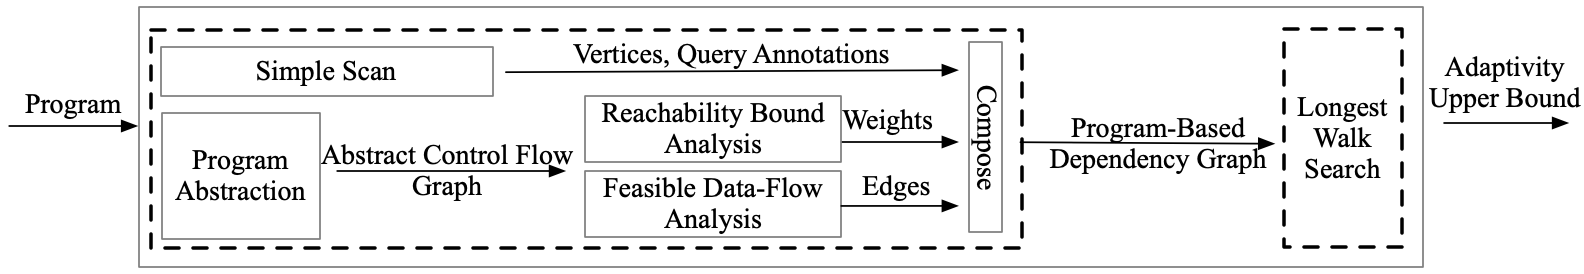
\includegraphics[width=1.0\columnwidth]{adapfun.png}
  \vspace{-0.3cm}
  \caption{The overview of {\THESYSTEM}}
  \label{fig:adaptfun}
  \vspace{-0.5cm}
\end{figure}
\subsubsection{Graph Estimation}
%
%
% \subsection{A guide to the algorithm}
% In order to have the upper bound of adaptivity:
% \\
% \begin{enumerate}
% \item $\THESYSTEM$  first builds a program-based dependency graph to {over-}approximate the
% % execution-based dependency graph (in Definition~\ref{def:trace_graph})
% Execution-Based Dependency Graph (in Definition~\ref{def:trace_graph})
% through Section~\ref{sec:alg_vertexgen}, Section~\ref{sec:alg_weightedgegen} and~\ref{sec:alg_graphgen}:
% % in the phases one to phases four of $\THESYSTEM$ in Section~\ref{sec:abscfg} to Section~\ref{sec:alg_graphgen}:
% \\
% 1.1 approximate the vertices: 
% % in the forth step of
% in the first phase of $\THESYSTEM$ in
% % the algorithm in Section~\ref{sec:alg_graphgen} 
% Section~\ref{sec:alg_vertexgen}
% without extra static analysis technique.
% \\
% 1.1 approximate the query annotations: 
% % in the forth step of
% in the first phase of $\THESYSTEM$ in
% % the algorithm in Section~\ref{sec:alg_graphgen} 
% Section~\ref{sec:alg_vertexgen}
% without extra static analysis technique.
% \\
% 1.2 approximate the vertices weights:
% in the second phase of 
% % the algorithm in  
% of $\THESYSTEM$ specifically in Section~\ref{sec:alg_weightgen}
% \\
% 1.3 approximate the edges between vertices:
% also in the second phase of $\THESYSTEM$ specifically in 
% % Section~\ref{sec:alg_weightgen}
% Section~\ref{sec:alg_edgegen}
% \\
% 1.4 generate the final approximated program-based dependency graph in Section~\ref{sec:alg_graphgen}
% %  to {over-}approximate the
% % approximate the query annotation: 
% % in the forth step of
% in the third phase of $\THESYSTEM$.
% % the algorithm  without extra static analysis technique.
% % \\
% This program-based graph has a similar topology structure as 
% % the one
% % of 
% the Execution-Based Dependency Graph. It has the same
% vertices and query annotations, but approximated edges and weights. 
% \item Then in the last phase in Section~\ref{sec:alg_adaptcompute}, $\THESYSTEM$
% % we compute the upper bound for adaptivity over this approximated graph:
% % , as an upper bound for
% % program's adaptivity
% computes the upper bound for adaptivity over this approximated graph.
% % in the last phase of this algorithm in Section~\ref{sec:alg_adaptcompute}.
% % \subsection{Adaptivity Based on Program Analysis in \THESYSTEM}
% % In order to give a bound on the program's adaptivity, we first build a
% % program-based data-dependency graph to {over-}approximate the
% % trace-based dependency graph.  Then, we define a program-based
% % adaptivity over this approximated graph, as an upper bound for
% % $A(c)$.
% \end{enumerate}
According to the dependency graph we use in adaptivity definition, we want to build a similar graph to {over-}approximate the
% execution-based dependency graph (in Definition~\ref{def:trace_graph})
Execution-Based Dependency Graph (in Definition~\ref{def:trace_graph}). The construction considers the vertices, edges, and the weight of every node, as well as some annotations which marks the query usage. The overall picture of this step is organized as follows.
% through Section~\ref{sec:alg_vertexgen}, Section~\ref{sec:alg_weightedgegen} and~\ref{sec:alg_graphgen}:


\begin{enumerate}
\item  Vertices are the assigned variables with unique labels, which is extracted directly from the program, see Section~\ref{sec:alg_vertexgen}
without extra static analysis technique
% \item Query annotations are also decided directly from the program, when there is a query request, the associated variables which are the results of the query requests are marked in the form of a flag, $0$ means no query, $1$ represents query related. See Section~\ref{sec:alg_vertexgen}.
\item The edge between vertices considers both control flow and data flow, See
Section~\ref{sec:alg_edgegen}
\item Every vertex and edge come with a weight, which tells the maximal times each vertex and edge can be visited in realistic execution. This weight is estimated by a reachability bound analysis on each vertex, See Section~\ref{sec:alg_weightgen}.
% \item Each edge also vertices considers both control flow and data flow, See
% Section~\ref{sec:alg_edgegen}
\item  Finally, with all the ingredients ready, we construct the final approximated program-based dependency graph in Section~\ref{sec:alg_graphgen}
\end{enumerate}

% the algorithm  without extra static analysis technique.
% \\
Overall, this program-based graph has a similar topology structure as 
% the one
% of 
the Execution-Based Dependency Graph. It has the same
vertices and query annotations, but approximated edges and weights. We call the graph generated by static analysis techniques, static analysis dedendency graph. 
% \item Then in the last phase in Section~\ref{sec:alg_adaptcompute}, $\THESYSTEM$
% % we compute the upper bound for adaptivity over this approximated graph:
% % , as an upper bound for
% % program's adaptivity
% computes the upper bound for adaptivity over this approximated graph.
% in the last phase of this algorithm in Section~\ref{sec:alg_adaptcompute}.
% \subsection{Adaptivity Based on Program Analysis in \THESYSTEM}
% In order to give a bound on the program's adaptivity, we first build a
% program-based data-dependency graph to {over-}approximate the
% trace-based dependency graph.  Then, we define a program-based
% adaptivity over this approximated graph, as an upper bound for
% $A(c)$.


\subsubsection{Adaptivity Computation}

Likewise the adaptivity is defined as a finite walk in the execution based depdenency graph, our static estimation on this adaptivity also relies on finding a path in the static analysis depdenency graph.   The construction of the stastic analysis dependency graph is of great value of showing some useful properties of the target program, such as dependency between variables, the execution upper bound of a certian command, while the key novelty is our path searching algorithm, which connects all the information we need in the static anlaysis dependency graph and provides us a sound over-estimation of adaptivity! In order to get a sound but precise upper bound, we will discuss some challenges in finding the 'appropriate' path in the graph, and how our algorithm responds to these challengs. We present the path seaching algorithm in Section~\ref{sec:alg_adaptcompute}.
 
% An
% approximated edge correspond to a program-based data dependency
% relation ($\flowsto$ in Definition~\ref{def:flowsto}) and an approximated
% weight corresponds to a reachability bound analysis results from
% Definition~\ref{def:transition_closure}.

% %
% \subsubsection{Program-Based Variable Dependency}
% The program-based dependency relation over two labeled variables ($x^i, y^j)$ is defined as a $\flowsto$ relation with respect to the program $c$ as follows.
% %
% \begin{defn}[Data Flow Relation between Assigned Variables ($\flowsto$)].
% \label{def:flowsto}
% \\
% Given a program  ${c}$,
% a variable ${x^i}  \in \lvar_c $ is in the \emph{flows to} relation with another variable ${y^j} \in \lvar_c$, if and only if:
% \mg{I cannot even parse the next formula. Why there is a big disjunction on the left? Disjunction is a binary operation, or n-ary if given a set, what is this disjunction between?}\\
% \mg{please, remove the underscript $c$ in the exists. It just makes everything mroe difficult to parse.}\\
% \mg{The use of $\lor$ is odd. E.g. $\exists {(\expr \lor \qexpr)}$ or
%   $ [{\assign{y}{\expr \lor \query(\qexpr)}}]^{j} $. I suggest to write the whole formula instead of using weird shortenings.}\\
% \mg{Also, now it is too late to change this but instead of breaking down the definition using the subterm relation and then defining the flowto relation, it would have been better to give just one inductive definition of Flowto - I imagine that this makes also the proof more awkward.}
% %
% {\footnotesize 
% \[
% \begin{array}{l}
% \flowsto({x^i, y^j, c}) \triangleq 
% \\
% \left( \bigvee
% \begin{array}{l}
% (\exists \expr \st \clabel{\assign{y}{\expr}}^j \in_{c} {c} 
% \land {x} \in FV(\expr) \land (x^i \in \live(j, c)))
% \\
% (\exists {\qexpr} \st [\assign{y}{\query({\qexpr})}]^j \in_{c} {c} 
% \land x \in FV({\qexpr}) \land (x^i \in \live(j,c))))
% \\
% \Big(\exists {c_w} \in \cdom, l \in \mathcal{L}, \bexpr \st
% 	\ewhile [\bexpr]^l \edo {c_w} \in_{c} {c}
% 	\land \flowsto(x^i, y^j, c_w)
% 	\\ \qquad	
%      \lor 
% 	\big( \exists {(\expr \lor \qexpr)} \st
% 	[{\assign{y}{\expr \lor \query(\qexpr)}}]^{j} \in_{c}  {c_w}  \land {x} \in FV(\bexpr) \land x^i \in \live(l, c)
% 	\big)
% 	\Big)
% \\
% \Big(
% \exists {c_1}, {c_2} \in \cdom, l \in \mathcal{L}, \bexpr 
% \st 
% 	\eif([\bexpr]^l, {c_1}, {c_2}) \in_{c} {c} \land
% 	\flowsto(x^i, y^j, c_1) \lor \flowsto(x^i, y^j, c_2)
% 	\\ \qquad 
% 	\lor 
% 	\big( \exists {(\expr \lor \qexpr)} \st
% 	\land {x} \in FV(\bexpr) \land x^i \in \live(l, c) \land
% 	([{\assign{y}{\expr \lor \query(\qexpr)}}]^{j} \in_{c}  {c_1}  
% 	\lor [{\assign{y}{\expr \lor \query(\qexpr)}}]^{j} \in_{c}  {c_2})
% 	\big)
% \Big)
% % \\
% \end{array}
% \right).
% \end{array}
% \]
% }
% %
% \end{defn}
% %
% \mg{The next notation is inconsistent with the one used above. Also, this definition should be given before the definition of flowto. From the description I have no cluse what this notion of reachability means. Also, the definition is referred to does not define this notation.}\\
% \mg{the definition somehow seems to make sense but until when the or notation is fixed and I don't see the definition of RD, I cannot tell for sure.}
% $\live^l(c) \subseteq \lvar_c$,
% which is the set of all the reachable variables at location of label $l$ in the program $c$.
% For every labelled variable $x^l$ in this set, 
% the value assigned to that variable
% in the assignment command associated to that label is reachable at the entry point of  executing the command of label $l$.
% This is formally defined , formally computed in Definition~\ref{def:feasible_flowsto}
% \\
% \mg{This description seems inconsistent with the definition. I suggest to use the same variables and terms.}
% To understand the $\flowsto$ intuition, 
% given a program  ${c}$ with its labelled variables $\lvar_c$, and two variables ${x^i}, y^j  \in \lvar_c $ 
% % showing up as $i$-th, $j$-th elements in $\lvar$ 
% % (i.e., ${x} = \lvar(i)$ and ${y} = \lvar(j)$),
% we say $y^j$ flows to ${x^i}$ in ${c}$ if and only if 
% the value of $y^j$ directly or indirectly influence the evaluation of the value of ${x}$ as follows:
% %
% \begin{itemize}
% \item (Explicit Influence) The program ${c}$ contains either 
% a command $[\assign{{x}}{\aexpr}]^i$ or $[\assign{{x}}{\query({\qexpr})}]^i$,
% such that ${y}$ shows up as a free variable in $\expr$ or ${\qexpr}$.
% We use $\flowsto({x^i, y^j, c})$ to denote $y^j$ flows to $x^i$ in ${c}$.
% %
% \item (Implicit Influence) The program ${c}$ contains either a while loop
% command
% or if command, 
% such that $x$ shows up in the guard
% and $y$ shows up in the left hand of an assignment command and this assignment command showing up
%  in the body of the while loop, or branches of if command.
% \end{itemize}
% %
% % This is formally defined in \ref{def:flowsto}.
% % We use $FV(\expr)$, $FV(\sbexpr)$ and $FV(\qexpr)$ denote the set of free variables in 
% % expression $\expr$, boolean expression $\sbexpr$ and query expression $\qexpr$ respectively.
% %
% %
% \mg{I don't understand what this definition of equivalence means. It is not observational equivalence
% and it is not syntactic equivalence. What are we trying to capture here? Also, it is equivalence of programs, not of program.}
% \begin{defn}[Equivalence of Program]
% %
% \label{def:aq_prog}
% Given 2 programs $c_1$ and $c_2$:
% \[
% c_1 =_{c} c_2
% \triangleq 
% \left\{
%   \begin{array}{ll} 
%     \etrue        
%     & c_1 = \eskip \land c_2 = \eskip
%     \\ 
%     \forall \trace \in \mathcal{T} \st \exists v \in \mathcal{VAL}
%     \st \config{ \trace, \expr_1} \aarrow v \land \config{ \trace, \expr_1} \aarrow v     
%     & c_1 = \assign{x}{\expr_1} \land c_2 = \assign{x}{\expr_2} 
%     \\ 
%     \qexpr_1 =_{q} \qexpr_2       
%     & c_1 = \assign{x}{\query(\qexpr_1)} \land c_1 = \assign{x}{\query(\qexpr_2)} 
%     \\
%     c_1^f =_{c} c_2^f \land c_1^t =_{c} c_2^t
%     & c_1 = \eif(b, c_1^t, c_1^f) \land c_2 = \eif(b, c_2^t, c_2^f)
%     \\ 
%     c_1' =_{c} c_2'         
%     & c_1 = \ewhile b \edo c_1' \land c_2 = \ewhile b \edo c_2'
%     \\ 
%     c_1^h =_{c} c_2^h \land c_1^t =_{c} c_2^t
%     & c_1 = c_1^h;c_1^t \land c_2 = c_2^h;c_2^t 
%   \end{array}
%   \right.
% \]
% %
% As usual, we denote by $c_1 \neq_{c} c_2$ the negation of the equivalence.
% %
% \end{defn}
% %
% \mg{This definition needs to go before it is used. }
% Given 2 programs $c$ and $c'$, we denote by $c' \in_{c} c$  that $c'$ is a sub-program of $c$ defined as follows,
% \begin{equation}
% c' \in_{c} c \triangleq \exists c_1, c_2, c''. ~ s.t.,~
% c =_{c} c_1; c''; c_2 \land c' =_{c} c''
% \end{equation} 
% %

% \subsubsection{Program Analysis Based Dependency Graph}
% We give the formal definition for the program-based dependency graph for a program $c$, 
% $\progG({c}) = (\vertxs, \edges, \weights, \flag)$ as follows.
% \begin{defn}
%     [Program-Based Dependency Graph].
%     \label{def:prog_graph}
%     \\
% Given a program ${c}$
% its program-based graph 
% $\progG({c}) = (\vertxs, \edges, \weights, \qflag)$ is defined as:
% {\footnotesize
% \[
% \begin{array}{rlcl}
% \text{Vertices} &
% \vertxs & := & \left\{ 
% x^l \in \mathcal{LV} 
% ~ \middle\vert ~
% x^l \in \lvar_{c}
% \right\}
% \\
% \text{Directed Edges} &
% \edges & := & 
% \left\{ 
%   ({x}_1^{i}, {x}_2^{j}) \in \mathcal{LV} \times \mathcal{LV}
%   ~ \middle\vert ~
%   \begin{array}{l}
%     {x}_1^{i}, {x}_2^{j} \in \vertxs
% 	\land
%     % \\
%     \exists n \in \mathbb{N}, z_1^{r_1}, \cdots, z_n^{r_n} \in \lvar_{{c}} \st 
%     n \geq 0 \land
%     \\
%     \flowsto(x^i,  z_1^{r_1}, c) 
%     \land \cdots \land \flowsto(z_n^{r_n}, y^j, c) 
%   \end{array}
% \right\}
% \\
% \text{Weights} &
% \weights & := &
% % \bigcup
% % \begin{array}{l}
% 	\left\{ (x^l, w) \in  \mathcal{LV} \times EXPR(\constdom)
% 	\mid
% 	x^l \in \lvar_{{c}} \land w = \absW(l)
% 	\right\}
% % \end{array} 
% \\
% \text{Query Annotation} &
% \qflag & := & 
% \left\{(x^l, n)  \in  \mathcal{LV} \times \{0, 1\} 
% ~ \middle\vert ~
%  x^l \in \lvar_{c},
% n = 1 \iff x^l \in \qvar_{c} \land n = 0 \iff  x^l \in \qvar_{c} .
% \right\}
% \end{array}
% \] 
% }
% , where the $\absW(l)$ is the symbolic reachability bound in domain of $EXPR(\constdom)$,
% % for the assignment command of label $l$ to which  
% the labeled variable $x^l$, 
% % is associated, 
% computed from the $\THESYSTEM$ algorithm 
% in Definition~\ref{def:transition_closure}.
% The $EXPR(\constdom)$ is an expression over symbolic constants containing the
% input variables and natural number.
% \end{defn} 
% %
% \paragraph{Program-Based Adaptivity ($\progA(c)$)}
% %
% Given a program ${c}$, we generate its program-based graph 
% $\progG({c}) = (\vertxs, \edges, \weights, \qflag)$.
% %
% Then the adaptivity bound based on program analysis for ${c}$ 
% % is the number of query vertices on a finite walk in $\progG({c})$. This finite walk satisfies:
% % \begin{itemize}
% % \item the number of query vertices on this walk is maximum
% % \item the visiting times of each vertex $v$ on this walk is bound by its reachability bound $\weights(v)$.
% % \end{itemize}
% is computed as the maximum query length over all finite walks in $\walks(\progG({c}))$,
% %
% % It is formally defined in \ref{def:prog_adapt}.
% defined formally as follows.
% %
% %
% \begin{defn}
% [{Program-Based Adaptivity}].
% \label{def:prog_adapt}
% \\
% {
% Given a program ${c}$ and its program-based graph 
% $\progG({c}) = (\vertxs, \edges, \weights, \qflag)$,
% %
% the program-based adaptivity for $c$ is defined as%
% \[
% \progA({c}) 
% := \max
% \left\{ \qlen(k)\ \mid \  k\in \walks(\progG({c}))\right \}.
% \]
% }
% \end{defn}  
%
%
% {
% \begin{defn}[Variable Flags ($\flag$)].
% \\
% Given a program  ${c}$ with its labelled variables $\lvar$, the $\flag$ is a vector of the same length as $\lvar$, s.t. for each variable ${x}$ showing up as the $i$-th element in $\lvar$ (i.e., ${x} = \lvar(i)$), 
% $\flag(i) \in \{0, 1, 2\}$ is defined as follows:
% %
% %
% \[
% \flag(i) := 
% \left\{
% \begin{array}{ll}
% 2 & 
% {x^l} \in \lvar_{c} \land 
% (\exists {\qexpr}. ~ s.t., ~
% [\assign{{x}}{\query({\qexpr})}]^l \in_{c} {c})
% \\
% 1 &  
% \begin{array}{l}
% {x^l} \in \lvar_{c} \bigwedge \\
% \left(
% \begin{array}{l}
% \big(\exists  ~ {c'}, {\expr}, \sbexpr, l, l'. ~
% 	\ewhile [\sbexpr]^l \edo {c'} \in_{c} {c}
% 	\land 
% 	[{\assign{x}{\expr}}]^{l'} \in_{c}  {c'}
% \big) \bigvee
% \\
% \big(\exists ~ \sbexpr, l, l_1, l_2, {c_1}, {c_2}, {\expr}_1, {\expr}_2. ~
% 	\eif([\sbexpr]^l, {c_1}, {c_2}) \in_{c} {c} \land
% 	([{\assign{x}{\expr_1}}]^{l1} \in_{c} {c_1} \lor 
% 	[{\assign{x}{\expr_2}}]^{l2} \in_{c} {c_2})
% \big)
% \end{array}
% \right)
% \end{array}
% \\
% 0 & \text{o.w.}
% \end{array}
% \right\}. 
% \] 
% %
% \end{defn}
%
% Operations on $\flag$ are defined as follows:
% \begin{equation}
% \begin{array}{llll}
% {\flag_1 \uplus \flag_2}(i) & := &
% \left\{
% \begin{array}{ll}
% k & k = \max{\big\{\flag_1(i), \flag_2(i)\big\}} 
% \land |\flag_1| = |\flag_2|\\
% 0 & o.w.
% \end{array}\right.
% & i = 1, \cdots, |\flag_1|  
% \\
% {\flag \uplus n}(i) & := & 
% \max\big\{ \flag(i), n \big\} 
% & i = 1, \ldots, |\flag|    
% \\
% \left[ n \right]^k (i) & := &  n
% & i = 1, \ldots, k ~ \land ~ |\left[ n \right]^k| = k
% \end{array}
% \end{equation}
%
%
%
% \begin{defn}[Data Flow Matrix ($\Mtrix$)]
% The data flow matrix $\Mtrix$ of a program $c$ is a matrix of size $|\lvar_c| \times |\lvar_c|$ 
% s.t.,
% %
% \[
% \Mtrix(i, j) \triangleq
% \left\{
% \begin{array}{ll}
% 1	&	\flowsto({x^i, y^j, c}) \\
% 0	& o.w.
% \end{array}
% \right., {x^i}, y^j  \in \lvar_c.
% \]
% %
% \end{defn}
% %
% Operations on the data flow matrices are defined as follows:
% %
% \begin{equation}
% \Mtrix_1 ; \Mtrix_2 
% := \Mtrix_2 \cdot \Mtrix_1 + \Mtrix_1 + \Mtrix_2
% \end{equation}
% %
% Consider the same program $c$ as above, its data flow matrix $\Mtrix$ and $\flag$ for the program $c$ is as follows:
% $$
% {c} = 
% \begin{array}{l}
% \left[{\assign {x_1} {\query(0)}}	\right]^1;
% \\
% \left[{\assign {x_2} {x_1 + 1}}		\right]^2;
% \\
% \left[{\assign {x_3} {x_2 + 2}}		\right]^3
% \end{array}
% ~~~~~~~~~~~~
% \Mtrix
% =  \left[ 
% \begin{matrix}
% 0 & 0 & 0 \\
% 1 & 0 & 0 \\
% 1 & 1 & 0 \\
% \end{matrix} \right] ~ , 
% \flag = \left [ \begin{matrix}
% 1 \\
% 0 \\
% 0 \\
% \end{matrix} \right ]
% $$
% %
% % There are two special matrices used for generating the data flow matrix $\Mtrix$ in the analysis algorithm. They are the left matrix $\lMtrix_i$ and right matrix $\mathsf{R_{(e, i)}}$.

% % Given a program  ${c}$ with its labelled variables $\lvar$ of length $N$,
% % the left matrix $\lMtrix_i$ generates a matrix of $1$ column, $N$ rows, 
% % where the $i$-th row is $1$ and all the other rows are $0$.
% % %
% % \begin{defn}[Left Matrix ($\lMtrix_i$)].
% % \\
% % Given a program  ${c}$ with its labelled variables $\lvar$ of size $N$, 
% % the left matrix $\lMtrix_i$ is defined as follows:
% % \[
% % \lMtrix_i(j) : = 
% % \left
% % \{
% % \begin{array}{ll}
% % 1 & j = i \\
% % 0 & o.w.
% % \end{array}
% % \right.,
% % j = 1, \ldots, N.
% % \]
% % \end{defn}
% % %
% % Given a program  ${c}$ with its labelled variables $\lvar$ of length $N$,
% % the right matrix $\rMtrix_{\expr, i}$ generates a matrix of one row and $N$ columns, 
% % where the locations of free variables in $\expr$ is marked as $1$. 
% % %
% % %
% % \begin{defn}[Right Matrix ($\rMtrix_{\expr}$)].
% % \\
% % Given a program  ${c}$ with its labelled variables $\lvar$ of length $N$, 
% % the right matrix $\rMtrix_{\expr}$ is defined as follows:
% % \[
% % \rMtrix_{\expr}(j) : = 
% % \left\{
% % \begin{array}{ll}
% % 1 & {x} \in FV(\expr) 
% % \\
% % 0 & o.w.
% % \end{array}
% % \right.,
% % {x} = \lvar(j) ~ , ~ j = 1, \ldots, N.
% % \]
% % %
% % %
% % \end{defn}
% % %
% % Using the same example program ${c}$ as above with labelled variables $\lvar = [ {x_1 , x_2 , x_3} ] $,
% % the left and right matrices w.r.t. its $2$-nd command 
% % $\left[{\assign {x_2} {x_1 + 1}}\right]^2$  are as follows:
% % \[
% % \lMtrix_1 = \left[ \begin{matrix}
% % 0   \\
% % 1 	 \\
% % 0   \\
% % \end{matrix}   \right ] 
% % ~~~~~~~~~~~~~~
% % \rMtrix_{{x}_1 + 1}
% % = \left[ \begin{matrix} 
% % 1 & 0 & 0 \\
% % \end{matrix}  \right]
% % \]
% %
% %
% %
% \subsection{ $\THESYSTEM$ Analysis Algorithm}
% \subsection{Dependency Graph Estimation}
\subsection{Vertices Estimationn}
\label{sec:alg_vertexgen}
The first component of every vertex in the static analysis dependency graph are actually identical as the  Execution-Based Dependency Graph, which are assigned variables in the program annotated with the unique label(line number). 
These vertices are collected by statically scanning the program, like what we do for vertices of its Execution-Based Dependency Graph. 
The vertices are defined formally as follows.

  \highlight{
\[
    \progV^0(c) \triangleq \left\{ 
  (x^l, w) \in \mathcal{LV} \times \mathcal{A}_{\lin}
  ~ \middle\vert ~
  x^l \in \lvar(c)
  \right\}
  \]
  }
  %
where $\mathcal{A}_{\lin}$ is the set of arithmetic expressions over $\mathbb{N}$ and program's input variables. 
The weight $w$ for every vertex will be computed in following step in Section~\ref{sec:alg_weightgen}.
% The static scanning of the programs also tells us whether one vertice(assigned variable) is assigned by a query request. We have similar definition when defining the Execution-Based Dependency Graph, 
% a set of pairs $\progF(c) \in \mathcal{P}(\mathcal{LV} \times \{0, 1\} )$ 
% % is the set of pairs 
% % The weight for each vertex in $\progV(c)$ is computed 
% mapping each $x^l \in \progV(c)$ to a flag, either $0$ or $1$, where $1$  means $x^{l}$ is a member of $ \qvar_{c}$, a set of those variables assigned with query requests, and $0$ means $x^{l}$ not in this set. It is defined formally below.

% \[\progF(c) =\left\{(x^l, n)  \in  \mathcal{LV} \times \{0, 1\} 
% ~ \middle\vert ~
% x^l \in \lvar_{c},
% n = 1 \iff x^l \in \qvar_{c} \land n = 0 \iff  x^l \not\in \qvar_{c} .
% \right\}\]
%

% \wq{To do: Add $\THESYSTEM$, a data flow analysis algorithm to scan the program and give a graph.}
% {\THESYSTEM} consists of three phases: 
% \begin{enumerate}
%     \item Generating an abstract control flow graph with each edge representing an abstract event transiting between two command labels. 
%     \item Computing the value bound invariant for each variable in the event and 
%     the event transition closure over the abstract control flow graph,
%     we get the reachability bound for each labeled command.
%     \item Refining the abstract control flow graph with data-flow, by performing the reaching definition analysis, we generate a weighted data control flow graph.
%     \item An algorithm to find the appropriate path in the weighted data control flow graph
% \end{enumerate}

% \begin{enumerate}
%     \item An algorithm to generate a precise data control flow graph
%     \item An algorithm to perform a Reachability number analysis to calculate the weight of each node in the graph generated in phase 1.
%     \item An algorithm to find the appropriate path in the weighted data control flow graph
% \end{enumerate}

\subsection{Edge and Weight Estimation}
\label{sec:alg_weightedgegen}

Since the edges of the execution-based graph of a program relies on the dependency relation, which handles both control flow and data flow, as an over-approximation of this graph, the edges of our static anlaysis dependency graph also covers these two kind of flows. We develop a feasible data flow relation to catch these two flows, in Section~\ref{sec:alg_edgegen}.


The weight of every vertice in the execution-based graph is built on all possible execution traces.
In order to over-approximate the weight statically but still tightly, we present a symbolic reachability bound analysis for estimation of the weight of each vertice(label) in Section~\ref{sec:alg_weightgen},
in spirit of some reachablility bound techiniques.


The edges and weight estimation are both performed on basis of an abstract control flow graph of the program, we first show how to generate this abstract execution control flow graph before the introduction of  the edge and weight estimation.  

% This analysis first 
%  generate an abstract control flow graph
%  over all program labels, 
% in order to analyzing the data flow relations through variables assigned in every labeled command,
% and the reaching time of each variable.
% Then, it refines this control flow graph 
% % into a weighted data-dependency graph, 
% and generate the Program-Based Dependency Graph,
% through the data flow and reaching bound analysis results.
% In the last step, it finds the longest finite walk in this weighted data control flow graph w.r.t. the query variables,
% and return the number of query vertices traversed alongside.
% % \wq{To do: Add $\THESYSTEM$, a data flow analysis algorithm to scan the program and give a graph.}
% To be more specific, {\THESYSTEM} consists of five phases as follows,
% \\
% % \jl{Better to have a graph or picture of overview of the algorithm}
% \todo{graph}
% \todo{pass again}
% This analysis
% \begin{enumerate}
%     % \item Generating 
%     \item first generate 
%     an abstract control flow graph
%     %  over all labels,
%     (remove?? with program's labels as vertices and abstract transitions as edges)
%     in Section~\ref{sec:abscfg},
%     % used to analyze 
%     for analyzing the weight of every vertex in $\progV(c)$ and edges between every vertex in $\progV(c)$ in the next two steps;
%     %  \ref{sec:alg_weightgen} and 
%     % \ref{sec:alg_edgegen}.

%     % which are used as program's control locations,
%     %
%     \item then use the abstract control flow graph generated above, 
%     compute the weight of every vertex in $\progV(c)$ by computing a symbolic reachability bound for each label in Section~\ref{sec:alg_weightgen},
%     % \\
%     \item and then use the same graph again to estimate the edges between every vertex in $\progV(c)$ by computing the feasible data flow relation between every labeled variables in Section~\ref{sec:alg_edgegen}.
  
% \end{enumerate}

\subsubsection{Abstract Execution Control Flow graph}
\label{sec:abscfg}
% In an 
%  % a program $c$ 
%  abstract control flow graph for a program $c$, $\absG(c)$, 
%  every 
%  vertex corresponds to the unique
%  label.
%  Specifically,
%  The edge is directed, 
%   representing an abstract transition 
%   between two control locations uniquely decided by the labels.   
%    (We refer control location and the label to the same thing). The abstract transition is of the form of a set of difference constraints for variables, built from the abstract execution trace of the program. For instance, the edge $(l_1, dc, l_2)$ from $l_1$ to $l_2$,
%   represents an abstract transition 
%   between two control locations with a set of difference constraints on it.
%  In this transition, the  command labeled with the second location $l_2$, 
%   will be executed after execution of the command with label $l_1$,
%  %  The abstract transition contains a set of difference constraints for variables, 
%  with the difference constraints generated by abstracting the command of the first label. Difference constraints is a constraint on difference between variables and constants, which will be formally introduced when we discuss experssion abstraction.
%  \wq{The edge in the abstract control flow graph comes from the abstract execution trace of the program. The abstract execution trace, an abstract representation of the execution, consists of a list of abstract transitions. Then, every abstract transition in the abstrction execution trace corresponds to an edge in the abstract control flow graph. In aonther word, the edge $(l_1, dc, l_2)$ in the abstract control flow graph, represents an abstract transition 
%   from $l_1$ to $l_2$, with a set of difference constraints $dc$. Also notice, the difference constraints generated during the abstract transition appears in the edge as annotation.}

%  % over program's abstract execution 

%  Overall, the key point of the abstract excution control flow graph is the construction of the abstract execution trace of a program, which relies on a program abstraction procedure in following steps:

%  \begin{enumerate}
%  \item  Computing the abstract expression for every assignment command in the program.
%  \item Computing the abstract event for every labeled command in the program. Intuitively, this abstract event aims 
%  to approximate the event in program's execution trace.
%  \item Constructing the abstract execution trace for a program.
%  \end{enumerate}  

We discuss the vertices and edge of the
abstract control flow graph for a program $c$, $\absG(c)$.

Every 
vertex corresponds to the unique
label.
Specifically,
the vertices of this graph is the set of $c$'s labels with an exit label $l_{ex}$, 
\[ 
  \absV(c) = labels(c)\cup\{l_{ex}\}
  \]
%  corresponding to a label command in the program.

% \wq{
  The edge in the abstract control flow graph comes from the abstract execution trace of the program. 
  The abstract execution trace, an abstract representation of the execution, consists of a list of abstract transitions. 
  Then, every abstract transition in the abstraction execution trace corresponds to an edge in the abstract control flow graph. In another word, the edge $(l_1, dc, l_2)$ in the abstract control flow graph, represents an abstract transition 
 from $l_1$ to $l_2$, with a set of difference constraints $dc$. 
 Also notice, the difference constraints generated during the abstract transition appears in the edge as annotation.
%  }

% over program's abstract execution 


% \wq{
  Overall, the vertices can be easily collected and the key point of construction of the abstract execution control flow graph for a program is the abstract execution trace, 
  which relies on the abstraction of expression and abstract transition (we also call it abstract event), we will discuss in the following section.
   To make it easy to understand, abstract control flow graph is a control flow graph, with difference constraints on every edge.
  % }  

%
\paragraph*{Expression Abstraction}

The expression assigned to the variable on the left hand of the assignment command is abstracted to an abstract value: (adopted from the expression abstraction method in paper \cite{sinn2017complexity}). The abstract value is expressed in the form of Difference constraint, denotated as $DC : \mathcal{VAR} \cup \constdom \to \mathcal{\mathcal{VAR} \times (\mathcal{VAR} \cup \constdom) } \times (\mathbb{Z} \cup \{\infty\})$.  $\constdom$ is called the Symbolic Constant defined as $\constdom \triangleq \mathbb{N} \cup \inpvar \cup \{\max{(\dbdom)}\} $, which consists of 
natural numbers $\mathbb{N}$,
the program's input variables $\inpvar$  
and a constant value $Q_m$ for estimating the upper bound of variables which are
assigned by queries. 

Give an instance of difference constraint used here,
$DC(\mathcal{VAR}  \cup \constdom) \cup \{\top\}$ represents all the difference constraints over 
variable and symbolic constants. 
% The difference constraint $DC$ over $\mathcal{VAR} \cup \constdom$ 
It is a set of the inequality of form $x \leq y + v$ where $x \in \mathcal{VAR} $, 
$y \in \mathcal{VAR}  \cup \constdom$ and $v \in \mathbb{Z}$. 
This difference constraint is defined in the same way as
\cite{sinn2017complexity}. For concise, we use $\dcdom^{\top}$ to represent the $DC(\mathcal{VAR}  \cup \constdom) \cup \{\top\}$ .


We show the expression abstraction $\absexpr : \expr \to \mathcal{VAR} \to DC(\mathcal{VAR}  \cup \constdom) \cup \{\top\} $ below.

% We introduce the following notations and operations first
% % an expression abstraction method based on the expression abstraction in paper \cite{sinn2017complexity}.
% \\
% % is enriched into $\constdom \triangleq \mathbb{N} \cup \inpvar \cup \{\max{(\dbdom)}\} $.
% T
% \\

% represents the set of inequality over all $\mathcal{VAR}  \cup \constdom$. 

% The symbolic constant is enriched into $\constdom \triangleq \mathbb{N} \cup \inpvar \cup \{\max{(\dbdom)}\} $.
% It consists of 
% natural number $\mathbb{N}$,
% the symbolic constants $\inpvar$ (i.e., the set of the program's input variables), 
% and a constant value $Q_m$ for estimating the upper bound of variables which are
% assigned by queries.
% \\
% The symbolic constant is enriched into $\constdom \triangleq \mathbb{N} \cup \inpvar \cup \{\max{(\dbdom)}\} $.
% \\

% % $ \absdom: \mathcal{P}(DC(\mathcal{VAR}  \cup \constdom) \cup \{\top \})$:
% \\
% $\constdom: \mathbb{N} \cup \inpvar \cup \{\max{(\dbdom)}\} $ 
% The  constant 
% \\
% % $DC(\mathcal{VAR}  \cup \constdom)$ represents the set of inequality over all $\mathcal{VAR}  \cup \constdom$.
% \\

% \[
%   \begin{array}{ll} 
%     \absexpr(y + c, x)  = x' \leq y + c  & c \in \mathbb{N} \land y \in (VAR \cup \constdom) \\
%     \absexpr(y - c, x)  = x' \leq y - c  & c \in \mathbb{N} \land y \in (VAR \cup \constdom) \\
%     \absexpr(v, x)  = x' \leq v + 0  & v \in (VAR \cup \constdom) \\
%     \absexpr(\aexpr, x) = x' \leq 0 + \infty   & \aexpr \text{ doesn't have any of the forms as above} \\
%     \absexpr(\qexpr, x)  = x' \leq 0 + Q_m & \qexpr \text{ is a query expression}  \\
%     \absexpr(\bexpr, x) = x' \leq 0 + 1   & \bexpr \text{ is a boolean expression} \\
%   \end{array}
%   \]
  \[
    \begin{array}{ll} 
      \absexpr(x - v, x)  = x' \leq x - v  & x \in \grdvar \land v \in \mathbb{N} \\
      \absexpr(y + v, x)  = x' \leq y + v  & x \in \grdvar \land v \in \mathbb{Z} \land y \in (\grdvar \cup \constdom) \\
      \absexpr(v, x)  = x' \leq v + 0  & x \in \grdvar \land v \in (\grdvar \cup \constdom) \\
      \absexpr(y + v, x)  = x' \leq y + v & \\
      \grdvar = \grdvar \cup \{y\} & x \in \grdvar \land v \in \mathbb{Z} \land y \notin (\grdvar \cup \constdom)  \\
      \absexpr(\qexpr, x)  = x' \leq 0 + Q_m & x \in \grdvar \land \qexpr \text{ is a query expression}  \\
      \absexpr(\bexpr, x) = x' \leq 0 + 1   & x \in \grdvar \land \bexpr \text{ is a boolean expression} \\
      \absexpr(\expr, x) = x' \leq \infty  &  x \in \grdvar \land \expr \text{ doesn't have any of the forms as above} \\
      \absexpr(\expr, x) = \top  &  x \notin \grdvar \\
    \end{array}
    \]
  
  % \wq{ 
    $\grdvar$ is the set of variables used in the guard expression of every while command in the program $c$. 
  % }. 
  In the case 4, if a variable $x$, belonging to the set 
  $\grdvar$ is updated by a variable $y$, which isn't in this set, 
  we add $y$ into the set $\grdvar$ and repeat 
  above procedure  until $\grdvar$ and $\absexpr(\expr, x)$ is stabilized. 
  % \wq{I do not understand this sentence:-(}
  \\
Specifically 
% understanding the intuition, 
we handle a 
% simplified 
normalized guard expression ($ x > 0$ for $x^l \in \lvar_c$)
 in $\ewhile$, and 
%  \wq{I do not understand this sentence:-(}
%  .
% \\
% The counter variables only increase, decrease or reset by expression in the form of arithmetic minus and plus (able to extend to max and min.)
the counter variables only increase, decrease or reset by 
% expression in the form of 
simple arithmetic expression (mainly multiplication, division, minus and plus (able to extend to max and min)). 
This is the same as in paper \cite{sinn2017complexity}. 
\\
For more complex expression assignments, where the counter reset, or calculated from $\elog$, 
multiplication or division, and expressions involving multiple variables, the constraint is approximated as reset of $\infty$.
\\
% This simplification \wq{which part we simplify here?} 
This approximation strategy
doesn't affect our analysis results in our examples. It is easy to extend the normalized expression 
into more complex forms as in \cite{sinn2017complexity}, as well as the 
counter variable manipulation with more advanced expressions.
% \\ 
% The boolean expression in the guard of $\ewhile$ command is normalized into form of $ x > 0$ where $x^l \in \lvar_c$ for some $l$.


\paragraph{Program Event Abstraction}
We show the abstract event definition, which is generated when computing its abstract execution trace.

\begin{defn}[Abstract Event]
  \label{def:abs_event}
  Abstract Event: 
  $\absevent \in $
  $\ldom \times \dcdom^{\top} \times \ldom$
  is a 
  % pair of abstract initial state and final state.
  triple where the first and third components are labels,
  second component is a constraint from $\dcdom^{\top}$.
  % the thrid % computed from program's abstract final and initial state, $\absfinal(c)$ and $\absinit(c)$ with formal definition, and algorithm detail in Appendix.
  %  the constraint and the third corresponds to a final state.
  \end{defn}
  Specifically, in an abstract event, 
  the first label correspond to an initial state, and 
  the second label and the constraint correspond to an abstract final state.
 The abstract initial state is a label from $\ldom$.
The abstract final state is a pair from $\ldom \times \dcdom^{\top}$,  
where first component is a label from $\ldom$ and the second component is a constraint from $\dcdom^{\top}$.
%

%
Given a program $c$, its abstract initial state,
and the set of its abstract final state is computed as follows,
%
\[
  \begin{array}{ll}
    \absinit(\clabel{\assign{x}{\expr}}{}^l)  & = l  \\
    \absinit(\clabel{\assign{x}{\expr}}{}^l)  & = l \\
    \absinit(\clabel{\eskip}^{l})  & = l \\
    \absinit(\eif [b]^l \ethen c_1 \eelse c_2)  & = l \\
    \absinit(\ewhile [b]^l \edo c)  & = l \\
    \absinit(c_1 ; c_2)  & = \absinit(c_1) \\
 \end{array}
 \]
%
Final State Abstraction: 
$\absfinal: \cdom \to \mathcal{P}(\ldom \times \dcdom^{\top})$,
computes the set of Abstract Final State for the command. 
 \[
  \begin{array}{ll}
    \absfinal(\clabel{\assign{x}{\expr}}{}^l)  & = \{(l, \absexpr\eapp (\expr, x))\}  \\
     \absfinal(\clabel{\assign{x}{\query(\qexpr)}}{}^l)  & = \{
      (l, x' \leq 0 + Q_m )\}  \\
     \absfinal(\clabel{\eskip}^{l})  
     & = \{(l, \top)\} \\
     \absfinal(\eif [b]^l \ethen c_1 \eelse c_2)  & = \absfinal(c_1) \cup \absfinal(c_2) \\
     \absfinal(\ewhile [b]^l \edo c)  & = \{(l, \top)\} \\
     \absfinal(c_1 ; c_2)  & =  \absfinal(c_2) \\
 \end{array}
 \]
 %
 \paragraph{Abstract Execution Trace}
 Now, we  extract the abstract execution trace  $\absflow(c)$ for a program, which computes the Abstract Execution Trace for program $c$, as a set of the abstract events $\absevent$.
 %
 \begin{defn}[Abstract Execution Trace]
 \label{def:abs_trace}
  $\absflow \in \cdom \to \mathcal{P}( \ldom \times DC(\mathcal{VAR}  \cup \constdom) \cup \{\top\}) \times \ldom )$
  \end{defn}
 %

 
  We now show how to compute the abstract execution trace. 
  For simplicity, we use $\mathcal{P}(\absevent)$ represent the power set of all abstract events, and we have $\absflow(c) \in \mathcal{P}(\absevent)$.
 We first append a skip command with 
%  a symbolic label $l_e$, i.e., $\clabel{\eskip}^{l_e}$ at the end of the program $c$, and compute the $\absflow(c) = \absflow'(c')$ for $c'$, where $c' = c;\clabel{\eskip}^{l_e}$ as follows,
the exist label $l_{ex}$, i.e., $\clabel{\eskip}^{l_{ex}}$ at the end of the program $c$, 
and compute the $\absflow(c) = \absflow'(c')$ for $c'$, where $c' = c;\clabel{\eskip}^{l_{ex}}$ as follows,
 %
 {\footnotesize
 \[
   \begin{array}{ll}
      \absflow'(\clabel{\assign{x}{\expr}}{}^l)  & = \emptyset  \\
      \absflow'(\clabel{\assign{x}{\query(\qexpr)}}{}^l)  & = \emptyset  \\
      \absflow'([\eskip]^{l})  & = \emptyset \\
      \absflow'(\eif [b]^l \ethen c_t \eelse c_f)  & =  \absflow'(c_t) \cup \absflow'(c_f)
      %   \\ & \quad 
        \cup \{(l, \top,  \absinit(c_t) ) ,  (l, \top, \absinit(c_f)) \} \\
       \absflow'(\ewhile [b]^l \edo c_w)  & =  \absflow'(c_w) \cup \{(l, \top, \absinit(c_w)) \} 
      %  \\ & \quad 
       \cup \{(l', dc, l)| (l', dc) \in \absfinal(c_w) \} \\
       \absflow'(c_1 ; c_2)  & = \absflow'(c_1) \cup  \absflow'(c_2) 
      %  \\ & \quad 
       \cup \{ (l, dc, \absinit(c_2)) | (l, dc) \in \absfinal(c_1) \} \\
   \end{array}
   \]
   }

   Notice $\absflow'([x := \expr]^{l})$, $\absflow'([x := \query(\qexpr)]^{l})$ and $\absflow'([\eskip]^{l})$ are all empty set. 
   For every event $\event$ with label $l$ in an execution trace $\trace$ of program $c$, 
   there is an abstract event in program's abstract execution trace of form $(l, \_, \_)$.  
   We also show the soundness of the abstract execution trace in Appendix.
  %  which says 
  %  \wq{...}
   \begin{lem}[Soundness of the Abstract Execution Trace]
     \label{lem:abscfg_sound}
   Given a program ${c}$, we have:
   %
   \[
     \begin{array}{l}
       \forall \vtrace_0, \trace \in \mathcal{T} ,  \event = (\_, l, \_) \in \eventset \st
   \config{{c}, \trace_0} \to^{*} \config{\eskip, \trace_0 \tracecat \vtrace} 
   \land \event \in \trace 
   \\
   \qquad \implies \exists \absevent = (l, \_, \_) \in (\ldom\times \dcdom^{\top} \times \ldom) \st 
   \absevent \in \absflow(c)
   \end{array}
   \]
   \end{lem}
%    This lemma is proved formally in Appendix~\ref{apdx:reachability_soundness}.
% For every event $\event$ with label $l$ in an execution trace $\trace$ of program $c$, 
% there is an abstract event in program's abstract execution trace of form $(l, \_, \_)$. 
This lemma is proved formally in Lemma~\ref{lem:abscfg_sound} in Appendix~\ref{apdx:reachability_soundness}.
\\
For every labeled variable in program $c$, $x^l \in \lvar_c$, there is a unique abstract event in program's abstract execution trace $\absevent \in \absflow(c)$ of form $(l, \_, \_)$. 
\begin{lem}[Uniqueness of the Abstract Execution Trace]
  \label{lem:abscfg_unique}
Given a program ${c}$, we have:
%
\[
  \begin{array}{l}
    \forall \vtrace_0, \trace \in \mathcal{T} ,  \event = (\_, l, \_, \_) \in \eventset^{\asn} \st
\config{{c}, \trace_0} \to^{*} \config{\eskip, \trace_0 \tracecat \vtrace} 
\land \event \in \trace 
\\
\qquad \implies \exists! \absevent = (l, \_, \_) \in (\ldom\times \dcdom^{\top} \times \ldom) \st 
\absevent \in \absflow(c)
\end{array}
\]
\end{lem}
This lemma and proof is also 
formalized in Lemma~\ref{lem:absevent_unique} in Appendix~\ref{apdx:reachability_soundness}.

Then, we build the edge for $c$'s abstract control flow graph as follos,
\[
  \absE(c) = \{(l_1, dc, l_2) | (l_1, dc, l_2) \in \absflow(c)\}
  \]

% We have a pre-processing algorithm to go through the programs and returns the list of labels associating with a loop and whose visiting times need to be analyzed.
%


\paragraph{Abstract Control Flow Graph} 
With the vertices $\absV(c)$ and edges $\absE(c)$ ready, we construct the abstract control flow graph, formally 
% Through a program $c$'s abstract execution trace, its abstract control flow graph is computed 
defined in 
Definition~\ref{def:abs_cfg}.
% Given program $c$ with its abstract control flow $\absflow(c)$, the Abstract Control Flow Graph:
% \\
\begin{defn}[Abstract Control Flow Graph]
\label{def:abs_cfg}
Given a program $c$, 
with its abstract control flow $\absflow(c)$
its abstract control flow graph $\absG(c) =(\absV(c), \absE(c), \absW(c))$ is defined as follows,
\\
% \highlight{
% :
%
% \\
$\absE(c) = \{(l_1, dc, l_2) | (l_1, dc, l_2) \in \absflow(c)\}$,
\\
$\absV(c) = labels(c)\cup\{l_{ex}\}$
\\
 $\absW(c) 
\triangleq \left\{ (l, w) \in \mathbb{L} \times EXPR(\constdom) \right\}$.
% }
% \\
% , where the weight of every label to be computed in the next step.
\end{defn}
% 
% The vertices $\absV(c)$ in this graph are program's labels with an exit label $l_{ex}$.
% Each directed 
%  edge $(l_1, dc, l_2)$ from $l_1$ to $l_2$,
%  represents an abstract transition 
%  between two control locations with a set of difference constraints on it.
% %  , i.e., the labels of two commands (we call the labels also control location and they refer to the same thing), 
% %  where 
% In this transition, the  command labeled with the second location $l_2$, 
%  will be executed after execution of the command with label $l_1$,
% %  The abstract transition contains a set of difference constraints for variables, 
% with the difference constraints generated by abstracting the command of the first label.
% % \\
% % It is easy to show for every $(l_1, dc, l_2) \in \absflow(c)$ such that $l_2 \neq l_e$, $(l_1, l_2) \in flow(c)$. The formal Lemma and proof can be found in Lemma~\ref{lem:flow_to_absflow} in Appendix~\ref{apdx:reachability_soundness}.
Notice we also define the $\absW(c)$ in this graph without giving an actual value.
This $\absW(c)$ is the set of weight for every 
% vertex 
label. The weight is a symbolic expression over the symbolic constant, 
which is the estimated upper bound on the number of visiting time for every control location
through the reachability bound analysis as follows.
%
% It is easy to show for every $(l_1, dc, l_2) \in \absflow(c)$ such that $l_2 \neq l_e$, $(l_1, l_2) \in flow(c)$. The formal Lemma and proof can be found in Lemma~\ref{lem:flow_to_absflow} in Appendix~\ref{apdx:reachability_soundness}.
%
\paragraph*{Example}
% Look at the two-round example again, its generated abstract control is shown as in Figure~\ref{fig:adapfun_tworound}(a).
% In this abstract control flow graph, every vertex is a label,
% corresponding to a label command in the program.
% Each directed 
% edge represents an abstract transition 
% between two control locations, 
% i.e., the labels of two commands (we call the labels also control location and they refer to the same thing), 
% where the second labeled command will be executed after execution of the command with first label.
% For example, the edge $0, a \leq 0, 1$ on the top, represents,
% from location $0$, the command 
% $\clabel{\assign{a}{0}}^0$ is executed with next continuation location $1$,
% where the 
% command $\clabel{\assign{j}{k}}^1$ will be executed next.
% The constraint $a \leq 0$ is generated by abstracting from the assignment command $\assign{a}{0}$,
% representing that value of $a$ is less than or equals to $0$ after 
% location $0$ before executing command at line $1$.
% %
% The same way for the rest edges' constructions.
%
Let us look at the two-round example, its generated abstract control flow graph is shown as in Figure~\ref{fig:abscfg_tworound}(b).
For example, the edge $(0, a \leq 0, 1)$ on the top, tells us the command 
$\clabel{\assign{a}{0}}^0$ is executed with next continuation location $1$,
where the 
command $\clabel{\assign{j}{k}}^1$ will be executed next.
The constraint $a \leq 0$ is a difference constraint, generated by abstracting from the assignment command $\assign{a}{0}$,
representing that value of $a$ is less than or equals to $0$ after 
location $0$ before executing command at line $1$. The difference constraint is an inequality relation between, the left-hand side of the inequality talks about the variable before the execution and the right-hand side ascribes those after the execution. 
Look at the $a < a+x $ on the edge $5$ to $2$, which describes the execution of the command at line $5$, which is an assignment $a = a+x$. The $a$ on the left side of $a < a+x$ represents the value of $a$ after the assignment, while the right-hand side $a$ stores the value before the assignment. 
Also, we have while loop, which is a circle $2 \to 4 \to 5 \to 2$ in Figure~\ref{fig:abscfg_tworound}(b). 
Please also look at the edge from $3$ to $4$, which talks about the query! The $x < Q_m$ describes the execution of a query request (the command at line 3), the query results stored in $x$ is bounded by $Q_m$. 
$Q_m$ is the maximal value for query requesting result from the database $DB$. $top$ means there is no assignment executed, for example, we have the difference constraint $\top$ on the edge $2$ to $6$, means at line $2$, there is no assignment (it is a testing guard $j>0$.) 
%
The same way for the rest edges' constructions.
\begin{figure} 
  \centering
  \begin{subfigure}{.2\textwidth}
  \begin{centering}
  {\small
  $
      \begin{array}{l}
            \clabel{ \assign{a}{0}}^{0} ;   
              \clabel{\assign{j}{k} }^{1} ; \\
              \ewhile ~ \clabel{j > 0}^{2} ~ \edo ~ \\
              \Big(
               \clabel{\assign{x}{\query(\chi[j])} }^{3}  ; \\
               \clabel{\assign{j}{j-1}}^{4} ;\\
              \clabel{\assign{a}{x + a}}^{5}       \Big);\\
              \clabel{\assign{l}{\query(\chi[k]*a)} }^{6}\\
          \end{array}
  $
  }
  \caption{}
  \end{centering}
  \end{subfigure}
    \begin{subfigure}{.35\textwidth}
    \begin{centering}
  %   \todo{abstract-cfg for two round}
  \begin{tikzpicture}[scale=\textwidth/20cm,samples=200]
  \draw[] (-7, 10) circle (0pt) node{{ $0$}};
  \draw[] (0, 10) circle (0pt) node{{ $1$}};
  \draw[] (0, 7) circle (0pt) node{\textbf{$2$}};
  \draw[] (0, 4) circle (0pt) node{{ $3$}};
  \draw[] (0, 1) circle (0pt) node{{ $4$}};
  \draw[] (-7, 1) circle (0pt) node{{ $5$}};
  % Counter Variables
  \draw[] (6, 7) circle (0pt) node {\textbf{$6$}};
  \draw[] (6, 4) circle (0pt) node {{ $ex$}};
  %
  % Control Flow Edges:
  \draw[ thick, -latex] (-6, 10)  -- node [above] {$a \leq 0$}(-0.5, 10);
  \draw[ thick, -latex] (0, 9.5)  -- node [left] {$j \leq k$} (0, 7.5) ;
  \draw[ thick, -latex] (0, 6.5)  -- node [left] {$\top$}  (0, 4.5);
  \draw[ thick, -latex] (0, 3.5)  -- node [right] {$x \leq Q_m$} (0, 1.5) ;
  \draw[ thick, -latex] (-0.5, 1)  -- node [above] {$j \leq j - 1$} (-6, 1) ;
  \draw[ thick, -latex] (-6, 1.5)  -- node [left] {$a \leq a + x$} (-0.5, 7)  ;
  \draw[ thick, -latex] (0.5, 7)  -- node [above] {$l \leq Q_m$}  (5.5, 7);
  \draw[ thick, -latex] (6, 6.5)  -- node [right] {$\top$} (6, 4.5) ;
  \end{tikzpicture}
  \caption{}
    \end{centering}
    \end{subfigure}
    \begin{subfigure}{.35\textwidth}
      \begin{centering}
    %   \todo{abstract-cfg for two round}
    \begin{tikzpicture}[scale=\textwidth/20cm,samples=200]
    \draw[] (-10, 10) circle (0pt) node{{ $0: 1$}};
    \draw[] (0, 10) circle (0pt) node{{ $1: 1$}};
    \draw[] (0, 7) circle (0pt) node{\textbf{$2: k$}};
    \draw[] (0, 4) circle (0pt) node{{ $3: k$}};
    \draw[] (0, 1) circle (0pt) node{{ $4: k$}};
    \draw[] (-10, 1) circle (0pt) node{{ $5: k$}};
    % Counter Variables
    \draw[] (6, 7) circle (0pt) node {\textbf{$6: 1$}};
    \draw[] (6, 4) circle (0pt) node {{ $ex: 1$}};
    %
    % Control Flow Edges:
  \draw[ thick, -latex] (-8, 10)  -- node [above] {$a \leq 0$}(-1.5, 10);
  \draw[ thick, -latex] (0, 9.5)  -- node [left] {$j \leq k$} (0, 7.5) ;
  \draw[ thick, -latex] (0, 6.5)  -- node [left] {$\top$}  (0, 4.5);
  \draw[ thick, -latex] (0, 3.5)  -- node [right] {$x \leq Q_m$} (0, 1.5) ;
  \draw[ thick, -latex] (-1.5, 1)  -- node [above] {$j \leq j - 1$} (-8, 1) ;
  \draw[ thick, -latex] (-8, 1.5)  -- node [left] {$a \leq a + x$} (-1.5, 7)  ;
  \draw[ thick, -latex] (1.5, 7)  -- node [above] {$l \leq Q_m$}  (4.5, 7);
  \draw[ thick, -latex] (6, 6.5)  -- node [right] {$\top$} (6, 4.5) ;
    \end{tikzpicture}
    \caption{}
      \end{centering}
      \end{subfigure}
  %       \begin{subfigure}{.3\textwidth}
  %   \begin{centering}
  %   \begin{tikzpicture}[scale=\textwidth/18cm,samples=200]
  % \draw[] (0, 10) circle (0pt) node
  % {{ $a^0: {}^1_{0}$}};
  % \draw[] (0, 7) circle (0pt) node
  % {\textbf{$x^3: {}^{k}_{1}$}};
  % \draw[] (0, 4) circle (0pt) node
  % {{ $a^5: {}^{k}_{0}$}};
  % \draw[] (0, 1) circle (0pt) node
  % {{ $l^6: {}^{1}_{1}$}};
  % % Counter Variables
  % \draw[] (5, 9) circle (0pt) node {\textbf{$j^2: {}^{1}_{0}$}};
  % \draw[] (5, 6) circle (0pt) node {{ $j^4: {}^{k}_{0}$}};
  % %
  % % Value Dependency Edges:
  % \draw[ ultra thick, -latex, densely dotted,] (0, 1.5)  -- (0, 3.5) ;
  % \draw[ ultra thick, -latex, densely dotted,] (0, 4.5)  -- (0, 6.5) ;
  % \draw[ thick, -latex] (0, 7.5)  -- (0, 9.5) ;
  % \draw[ thick, -Straight Barb] (1.5, 3.5) arc (120:-200:1);
  % \draw[ thick, -Straight Barb] (6.5, 6.5) arc (150:-150:1);
  % \draw[ thick, -latex] (5, 6.5)  -- (5, 8.5) ;
  % % Control Dependency
  % \draw[ thick,-latex] (1.5, 7)  -- (4, 9) ;
  % \draw[ thick,-latex] (1.5, 4)  -- (4, 9) ;
  % \draw[ thick,-latex] (1.5, 7)  -- (4, 6) ;
  % \draw[ thick,-latex] (1.5, 4)  -- (4, 6) ;
  % \end{tikzpicture}
  % \caption{}
  %   \end{centering}
  %   \end{subfigure}
    \vspace{-0.3cm}
    \caption{(a) The same $\kw{towRounds(k)}$ program as Figure~\ref{fig:overview-example}
    (b) The abstract control flow graph for $\kw{towRounds(k)}$  (c) The abstract control flow graph with the reachability bound for $\kw{towRounds(k)}$.}
    \vspace{-0.5cm}
    \label{fig:abscfg_tworound}
  \end{figure}
%

\subsubsection{\highlight{Edge Estimation with Interprocedure Call}}
\label{sec:alg_edgegen}
% \wq{
  We show how to estimate the directed edges in the static analysis dependency graph.
We develop a variant of data flow analysis, called Feasible Data-Flow Generation, which 
considers both the control flow and data flow and
is a sound approximation of the edges in the execution based dependency graph.
% }

% \wq{
  Also, worth to mention, we use the result of reaching definition on the abstract control flow graph in feasible 
data-flow generation to have a more precise approximation. Let us see a simple example, a program $ [x = 0]^{1}; [x=2]^{2};  [y = x+1]^{3}$. The standard data flow analysis 
tells us that both the labeled variable $x^{1}$ and $x${2} may flow to $y^{3}$, which will result in an unnecessary edge ($x^{1}, y^{3}$). The result of reaching definition 
can help us eliminate this kind of edge by telling us, at line $3$, only variable $x^{2}$ is reachable. 
% }


% In this step, through 
% % the vertices and edges in 
% $c$'s abstract contrl flow graph $\absG(c)$,
%  $\THESYSTEM$ performs a feasible data-flow analysis 
%  using the reachable definition algorithm,
% %  and then Then we generated the set of feasible data-flow between labeled variables based on that.
% and generates the 
% %set of 
% feasible data-flow relation between labeled variables.
% \\
%  By generating set of all the reachable variables at location of label $l$ in the program $c$.
% For every labelled variable $x^l$ in this set, 
% the value assigned to that variable
% in the assignment command associated to that label is reachable at the entry point of  executing the command of label $l$.
% \\
In the first step, 
it performs the standard reaching definition analysis given a program $c$, 
on 
% its every label $l$
every label in $\absV(c)$.  This step generates set of all the reachable variables at location of label $l$ in the program $c$.
The $\live(l, c)$ represent the analysis result, which is the set of 
reachable labeled variables in program $c$ at the location of label $l$.
For every labelled variable $x^l$ in this set, 
the value assigned to that variable
in the assignment command associated to that label is reachable at the entry point of  executing the command of label $l$.
% \\
% it performs the standard reaching definition analysis given a program $c$, on its every label $l$.
% \\
% Another operator \mathsf{blocks} 
The block, 
is either the command of the form of assignment, skip, or a test of the form of $[b]^{l}$, 
% and $block$ of program $c$ is 
denoted by $\mathsf{blocks}(c)$
the set of all the blocks 
in program $c$, where  $\mathsf{blocks}: \cdom \to \mathcal{P}(\cdom \cup \clabel{\bexpr}^{l})$.
Then it generates the set of feasible data-flow between labeled variables with detail in Definition~\ref{def:feasible_flowsto}, 
based on $\live(l, c)$ for every label in a program $c$ and its blocks $\mathsf{blocks}$.
\\
The details are as follows.
%
% Performing a feasible data-flow analysis through the reachable definition algorithm. 
%  By generating set of all the reachable variables at location of label $l$ in the program $c$.
% For every labelled variable $x^l$ in this set, 
% the value assigned to that variable
% in the assignment command associated to that label is reachable at the entry point of  executing the command of label $l$.
% \paragraph{Generate CFG}
%  \begin{def}
%   \label{def:init_label}
%   Define $\mathsf{init}$: Command -> label, which returns the initial label of the statement. 
% \[
%  \begin{array}{ll}
%     init([x := e]^{l})  & = l  \\
%      init([x := q(e)]^{l})  & = l \\
%      init([skip]^{l})  & = l \\
%      init([if [b]^l then C_1 else C_2]^{l})  & = l \\
%      init([while [b]^l do C]^{l})  & = l \\
%      init(C_1 ; C_2)  & = init(C_1) \\
%  \end{array}
%  \]
% \end{def}
%   Define $\mathsf{final}$: Command -> Powerset(label), which returns the final labels of the statement. 
%  \[
%  \begin{array}{ll}
%     final([x := e]^{l})  & = \{l\}  \\
%      final([x := q(e)]^{l})  & = \{l\}  \\
%      final([skip]^{l})  & = \{l\} \\
%      final([if [b]^l then C_1 else C_2]^{l})  & = final(C_1) \cup final(C_2) \\
%      final([while [b]^l do C]^{l})  & = \{l\} \footnote{while terminates after b evaluates to false} \\
%      final(C_1 ; C_2)  & =  final(C_2) \\
%  \end{array}
%  \]
% \paragraph*{Blocks and Defs}
%  Define block B to be either the command of the form of assignment, skip, or test of the form of $[b]^{l}$.\\
%  Define $\mathsf{blocks}$ : command -> Powerset(Block)
%  \[
%  \begin{array}{ll}
%     blocks([x := e]^{l})  & = \{[x := e]^{l}\}  \\
%      block([x := q(e)]^{l})  & = \{[x := q(e)]^{l}\}  \\
%      blocks([skip]^{l})  & = \{[skip]^{l}\} \\
%      blocks([if [b]^l then C_1 else C_2]^{l})  & = {[b]^{l}} \cup blocks(C_1) \cup blocks(C_2) \\
%      blocks([while [b]^l do C]^{l})  & = \{[b]^{l}\} \cup blocks(C) \\
%      blocks(C_1 ; C_2)  & = blocks(C_1) \cup  blocks(C_2) \\
%  \end{array}
%  \]
%  Define $\mathsf{labels}$ to get the labels of blocks.
%  \[
%    labels(C) = \{l | [B]^{l} \in blocks(C) \}
%  \]  

% The control flow graph is generated by edges between labels. Define $\mathsf{flow}$: command -> P (label $\times$ label ).

% \[
%  \begin{array}{ll}
%     flow([x := e]^{l})  & = \emptyset  \\
%      flow([x := q(e)]^{l})  & = \emptyset  \\
%      flow([skip]^{l})  & = \emptyset \\
%      flow([if [b]^l then C_1 else C_2)  & =  flow(C_1) \cup flow(C_2)\cup \{(l, init(C_1)) , (l, init(C_2)) \} \\
%      flow([while [b]^l do C)  & =  flow(C) \cup \{(l, init(C)) \} \cup \{(l', l)| l' \in final(C) \} \\
%      flow(C_1 ; C_2)  & = flow(C_1) \cup  flow(C_2) \cup \{ (l,init(C_2)) | l \in final(C_1) \} \\
%  \end{array}
%  \]
 
 \paragraph{Reaching definition analysis}
%  Define block B to be either the command of the form of assignment, skip, or test of the form of $[b]^{l}$.\\
%  Define $\mathsf{blocks}$ : command -> Powerset(Block)
A block  is either the command of the form of assignment, skip, or test of the form of $[b]^{l}$.\\
The operator $\mathsf{blk} : \cdom \to blocks$ gives all the blocks in program $c$.
\\
%  \[
%  \begin{array}{ll}
%     blocks([x := e]^{l})  & = \{[x := e]^{l}\}  \\
%      block([x := q(e)]^{l})  & = \{[x := q(e)]^{l}\}  \\
%      blocks([skip]^{l})  & = \{[skip]^{l}\} \\
%      blocks([if [b]^l then C_1 else C_2]^{l})  & = {[b]^{l}} \cup blocks(C_1) \cup blocks(C_2) \\
%      blocks([while [b]^l do C]^{l})  & = \{[b]^{l}\} \cup blocks(C) \\
%      blocks(C_1 ; C_2)  & = blocks(C_1) \cup  blocks(C_2) \\
%  \end{array}
%  \]
 Set $?$ to be undefined:
 \\
%  $label^{?}$ is label $\cup \{?\}$.\\
%  Define $\mathsf{kill}$: $blocks \to \mathcal{P}(\mathcal{VAR} \times LABEL \cup \{?\})$, which produces the set of labelled variables of assignment destroyed by the block.
The operator $\mathsf{kill}$: $blocks \to \mathcal{P}(\mathcal{VAR} \times \ldom \cup \{?\})$ produces the set of labelled variables of assignment destroyed by the block.
 \\
  % Define $\mathsf{gen}$: $blocks \to \mathcal{P}(\mathcal{VAR} \times LABEL \cup \{?\})$, which generates the set of labelled variables generated by the block.
  The operator $\mathsf{gen}$: $blocks \to \mathcal{P}(\mathcal{VAR} \times \ldom \cup \{?\})$ generates the set of labelled variables generated by the block.
  \\
  % Define $defs(x)(c): \mathcal{VAR} \to LABEL$, gives all the labels where assigns value to variable x in the target program $c$. 
  % The operator  $defs(c): \mathcal{VAR} \to \ldom$ gives all the labels where assigns value to variable in $c$. 
%  \[
%  \begin{array}{ll}
%     kill([x := e]^{l})  & = \{ (x, ?) \} \cup \{ (x, l') | l' \in defs(x) \} \\
%      kill([x := q(e)]^{l})  & = \{ (x, ?) \} \cup \{ (x, l') | l' \in defs(x) \}  \\
%      kill([skip]^{l})  & = \emptyset \\
%      kill([ [b]^l ]^{l})  & =  \emptyset
%  \end{array}
%  ~~
%   \begin{array}{ll}
%       gen([x := e]^{l})  & = \{ (x, l) \}  \\
%      gen([x := q(e)]^{l})  & = \{ (x, l) \}  \\
%      gen([skip]^{l})  & = \emptyset \\
%      gen([ [b]^l ]^{l})  & =  \emptyset 
%  \end{array}
%  \]
%  Define $in(l)$, $out(l)$: LABEL$ \to \mathcal{VAR} \times LABEL \cup \{?\}$ for every block in program $c$ is computed as follows,
%  \[
%  \begin{array}{lll}
%     in(l)  & = \{ (x, ?) | x^l \in \lvar_c \land  l = \absinit(c) \}  
%     \cup \{ out(l')|  | (l',\_, l) \in \absE \land  l \neq \absinit(c)\}  \\
%      out(l)  & =  gen(B^{l}) \cup \{ in(l) \setminus kill(B^l)  \} & B^l \in blocks(c)   
%  \end{array}
%  \]
%  computing $in(l)$ and $out(l)$ for every $B^l \in blocks(c) $, and repeating these two step
% until the $in(l)$ and $out(l)$ are stabilized for every $B^l \in blocks(c) $
% We use $\live_{in}(l,c)$ and $\live_{out}(l, c)$ denote the stabilized results for the command of label $l$ in program $c$. 
%  Define $defs(x)(c): \mathcal{VAR} \to LABEL$, gives all the labels where assigns value to variable x in the target program $c$.
% Define $defs(x)(c): \mathcal{VAR} \to \ldom$, gives all the labels where assigns value to variable x in the target program $c$.
% \\
%  Define $in(l)$, $out(l)$: $ \ldom \to \mathcal{VAR} \times LABEL \cup \{?\}$ for every block in program $c$ is computed as follows,
The operator  $in(l)$, $out(l)$: $ \ldom \to \mathcal{LV} \cup \{?\}$ for every block in program $c$ is defined as follows,
 \[
 \begin{array}{ll}
    % in(l)  & = \{ (x, ?) | x^l \in \lvar_c \land  l = \absinit(c) \}  
    in(l)  & = \{ x^{?} | x^l \in \lvar_c \land  l = \absinit(c) \}  
    \cup \{ out(l')|  | (l',\_, l) \in \absE(c) \land  l \neq \absinit(c)\}  \\
     out(l)  & =  gen(B^{l}) \cup \{ in(l) \setminus kill(B^l)  \}  
 \end{array}
 \]
computing $in(l)$ and $out(l)$ for every $B^l \in blocks(c) $, and repeating these two steps
until the $in(l)$ and $out(l)$ are stabilized for every $B^l \in blocks(c) $
% We use $\live_{in}(l,c)$ and $\live_{out}(l, c)$ denote the stabilized results for the command of label $l$ in program $c$. 
We use $\live(l,c)$ to represent 
% $\live_{in}(l,c)$ in the other part of the paper.
denote the stabilized result of $in(l)$ at label $l$ in program $c$. 
% The $\live_{in}(l,c)$ and $\live_{out}(l, c)$ is computed by the Standard worklist algorithm. (For simplicity, we use $\live(l,c)$ to represent $\live_{in}(l,c)$ in the other part of the paper.}
\\
% The $\live_{in}(l,c)$ and $\live_{out}(l, c)$ 
The stabilized $in(l)$ and $out(l)$ for program $c$, as well as $\live(l, c)$,
is computed by the standard worklist algorithm with detail as below. 
% For simplicity, we use $\live(l,c)$ to represent $\live_{in}(l,c)$ in the other part of the paper.
\begin{enumerate}
    \item initial in[l]=out[l]=$\emptyset$
    \item initial in[entry label] = $\emptyset$
    \item initialize a work queue, contains all the blocks in C
    \item while |W| != 0 \\
         pop l in W\\
          old = out[l]\\
          in(l) =  out(l') where $(l',\_, l) \in \absE(c)$\\
           out(l) = gen($b^l$) $\cup$ (in(l) - kill($b^l$) ) where $b^l$ in $\mathsf{blk}(c)$   \\
          if (old != out(l)) W= W $\cup$ \{l'| (l,l') in $(l',\_, l) \in \absE(c)$\}\\
          end while
\end{enumerate}
%
% computing $in(l)$ and $out(l)$ for every $B^l \in blocks(c) $, and repeating these two step
% until the $in(l)$ and $out(l)$ are stabilized for every $B^l \in blocks(c) $
% We use $\live_{in}(l,c)$ and $\live_{out}(l, c)$ denote the stabilized results for the command of label $l$ in program $c$. 
% The $\live_{in}(l,c)$ and $\live_{out}(l, c)$ is computed by the Standard worklist algorithm. (For simplicity, we use $\live(l,c)$ to represent $\live_{in}(l,c)$ in the other part of the paper.
%%
\paragraph{Feasible Data-Flow Generation}
by using the results of Reaching definition analysis results, specifically $\live(l, c)$ for every label in a program $c$, we refine the vertices and edges in the $\absG$ graph 
by generating the set of feasible data-flow between labeled variables as follows,
%
%   \[
%  \begin{array}{ll}
%     dcdg([x := e]^{l})  & = \{ (y^i, x^l) | y \in VAR(e) \land (y,i) \in \live_{in}(l) \}  \\
%      dcdg([x := q(e)]^{l})  & = \{ (y^i, x^l) | y \in VAR(e) \land (y,i) \in \live_{in}(l) \}  \\
%      dcdg([skip]^{l})  & = \emptyset \\
%      dcdg([if [b]^l then C_1 else C_2)  & =  dcdg(c_1) \cup dcdg(c_2)\\ & \cup \{(x^i,y^j) | x \in VAR(b) \land (x,i) \in \live_{in}(l) \land ([y = \_]^j) \in blocks(c_1) \} \\
%      &\cup \{(x^i,y^j) | x \in VAR(b) \land (x,i) \in \live_{in}(l) \land ([y = \_]^j) \in blocks(c_2) \} \\
%      dcdg([while [b]^l do c)  & =  dcdg(c) \cup \{(x^i,y^j) | x \in VAR(b) \land (x,i) \in \live_{in}(l) \land ([y = \_]^j) \in blocks(C) \} \\
%      dcdg(c_1 ;c_2)  & = dcdg(c_1) \cup  dcdg(c_2) \\
%  \end{array}
%  \]
%
\begin{defn}[Feasible Data-Flow]
  \label{def:feasible_flowsto}
  Given a program $c$ and two labeled variables $x^i, y^j$  in this program, 
  $\flowsto(x^i, y^j, c)$ is 
    {\footnotesize
    \[
   \begin{array}{ll}
    \flowsto(x^i, y^j, \clabel{\assign{x}{\expr}}{}^l)  & \triangleq (x^i, y^j) \in \{ (y^i, x^l) | y \in \mathsf{FV}(\expr) 
    % \land (y,i) \in \live(l, \clabel{\assign{x}{\expr}}^l) \}  \\
    \land y^i \in \live(l, \clabel{\assign{x}{\expr}}^l) \}  \\
    \flowsto(x^i, y^j, \clabel{\assign{x}{\query(\qexpr)}}{}^l)  & \triangleq (x^i, y^j) \in \{ (y^i, x^l) | y \in \mathsf{FV}(\qexpr) 
    % \land (y,i) \in \live(l,\clabel{\assign{x}{\query(\qexpr)}}^l) \}  \\
    \land y^i \in \live(l,\clabel{\assign{x}{\query(\qexpr)}}^l) \}  \\
    \flowsto(x^i, y^j, [\eskip]^{l})  & = \emptyset \\
    \flowsto(x^i, y^j, \eif ([b]^l, c_1, c_2))  & \triangleq \flowsto(x^i, y^j, c_1) \lor \flowsto(x^i, y^j, c_2) \\ 
        & \lor (x^i, y^j) \in
       \{(x^i,y^j) | x \in \mathsf{FV}(b) \land 
      %  (x,i) 
      x^i \in \live(l, \eif ([b]^l, c_1, c_2)) \land  y^j \in \lvar(c_1) \\
    %   ([y = \_]^j) \in \mathsf{blk}(c_1) \} \\
       &\lor (x^i, y^j) \in \{(x^i,y^j) | x \in \mathsf{FV}(b) \land 
      %  (x,i) 
      x^i\in \live(l, \eif ([b]^l, c_1, c_2))  \land  y^j \in \lvar(c_2) \\
    %   \land ([y = \_]^j) \in \mathsf{blk}(c_2) \} \\
       \flowsto(x^i, y^j, \ewhile [b]^l \edo c_w)  & \triangleq  \flowsto(x^i, y^j, c_w)  \lor
       \\ & 
       (x^i, y^j) \in  \{(x^i,y^j) | x \in \mathsf{FV}(b) \land 
      %  (x,i) 
      x^i \in \live(l,   \ewhile [b]^l \edo c_w) \land  y^j \in \lvar(c_w) \\
    %   ([y = \_]^j) \in \mathsf{blk}(c_w) \} \\
       \flowsto(x^i, y^j, c_1 ;c_2)  & \triangleq \flowsto(x^i, y^j, c_1) \lor \flowsto(x^i, y^j, c_2) \\
       {\highlight{\clabel{\efun}^l: x(r, x_1, \ldots, x_n) := c}}& \emptyset\\
       {\highlight{\clabel{\assign{x}{\ecall(f, e_1, \ldots, e_n)}}^l } } 
       &     
       \triangleq
       \flowsto(x^i, y^j, \clabel{\assign{x_i}{e_i}}^{(l,i)}) \lor
       \flowsto(x^i, y^j, \clabel{c^{+n}}^l) \lor 
       \flowsto(x^i, y^j, \clabel{\assign{x}{r^{{l_r}+n}}}^{l}) 
       \\ &
       \land
       f(r^{l_r}, x_1, \ldots, x_n) := c\in \live(l, c)
   \end{array}
   \]
   }
   \end{defn}
%
We prove that this \emph{Feasible Data-Flow} relation is a sound approximation 
of the \emph{Variable May-Dependency} relation over labeled variables for every program,
in Appendix~\ref{apdx:flowsto_soundness_extend}.
%
\paragraph*{Edges Estimation}
Then we define the estimated directed edges
% for each vertex in $\progV(c)$,
between vertices $({x}_1^{i}, w_1)$  
and $({x}_2^{j}, w_2)$ 
where ${x}_1^{i}, {x}_2^{j} \in \lvar(c)$,
as a set of triples 
% $\progW(c) \in \mathcal{P}(\mathcal{LV} \times \mathcal{LV} \times EXPR(\constdom))$ 
$\progE(c) \in \mathcal{P}(\mathcal{LV} \times \mathcal{A}_{\lin} \times \mathcal{LV})$
% is the set of pairs 
% The weight for each vertex in $\progV(c)$ is computed 
indicating a directed edge from the first vertex to the second one in each pair
as follows,
\highlight{
  \[
    \progE^0(c) \triangleq 
    \left\{ 
    ({x}_1^{i}, w, {x}_2^{j}) \in \mathcal{LV} \times 
    \mathcal{A}_{\kw{in}} \times \mathcal{LV}
    ~ \middle\vert ~
    \begin{array}{l}
      {x}_1^{i}, {x}_2^{j} \in \lvar(c)
    \land
      % \\
      \exists n \in \mathbb{N}, z_1^{r_1}, \cdots, z_n^{r_n} \in \lvar_{{c}} \st 
      n \geq 0 \land
      \\
      \flowsto(x^i,  z_1^{r_1}, c) 
      \land \cdots \land \flowsto(z_n^{r_n}, y^j, c) 
    \end{array}
    \right\}
    \]
}
The weight for every edge will be computed as next step in Section~\ref{sec:alg_weightgen}.
We prove that this estimated directed edge set $\progE(c)$ is a sound approximation of the 
edge set in $c$'s Execution-Based Dependency Graph 
in Appendix~\ref{apdx:adapt_soundness}.
%  \begin{defn}[Feasible Data-Flow]
%   \label{def:feasible_flowsto}
%     {\footnotesize
%     \[
%    \begin{array}{ll}
%       dcdg(\clabel{\assign{x}{\expr}}{}^l)  & = \{ (y^i, x^l) | y \in FV(e) \land (y,i) \in \live_{in}(l, \clabel{\assign{x}{\expr}}^l) \}  \\
%        dcdg(\clabel{\assign{x}{\query(\qexpr)}}{}^l)  & = \{ (y^i, x^l) | y \in FV(e) \land (y,i) \in \live_{in}(l,\clabel{\assign{x}{\query(\qexpr)}}^l) \}  \\
%        dcdg([\eskip]^{l})  & = \emptyset \\
%        dcdg([\eif [b]^l \ethen c_1 \eelse c_2)  & =  dcdg(c_1) \cup dcdg(c_2)\\ & \cup 
%        \{(x^i,y^j) | x \in FV(b) \land (x,i) \in \live_{in}(l) \land ([y = \_]^j) \in blocks(c_1) \} \\
%        &\cup \{(x^i,y^j) | x \in FV(b) \land (x,i) \in \live_{in}(l) \land ([y = \_]^j) \in blocks(c_2) \} \\
%        dcdg([\ewhile [b]^l \edo c)  & =  dcdg(c) \cup \{(x^i,y^j) | x \in FV(b) \land (x,i) \in \live_{in}(l) \land ([y = \_]^j) \in blocks(C) \} \\
%        dcdg(c_1 ;c_2)  & = dcdg(c_1) \cup  dcdg(c_2) \\
%    \end{array}
%    \]
%    }
%    \end{defn}
%    For any two labeled variables $x^i, y^j$ in a program $c$, 
%   %  it is easy to see that there is a one-on-one correspondence between 
%   %  $\flowsto$ relation of the two variables, and the $dcdg$ analysis result on $c$.
%   we use $\flowsto()$ denote if they have a feasible data-flow relation in Definition~\ref{def:flowsto}.
%    \begin{defn}[Feasible Data-Flow ($\flowsto$)]
%    \label{def:flowsto}
%    \[
%    \forall c \in \cdom, x^i, y^j \in \lvar_c \st 
%    \flowsto(x^i, y^j, c) \iff (x^i, y^j) \in dcdg(c)
%    \]
%    \end{defn}
  %  This soundness is proved in Proof~\ref{pf:rd_soundness} in Appendix~\ref{apdx:rd_soundness}.
  %  For any two labeled variables in a program $c$, it is easy to see that there is a one-on-one correspondence between 
  %  $\flowsto$ relation of the two variables, and the $dcdg$ analysis result on $c$.
  %  \begin{thm}[Soundness of the Feasible Data-Flow Analysis]
  %  \label{thm:rd_soundness}
  %  \[
  %  \forall c \in \cdom, x^i, y^j \in \lvar_c \st 
  %  \flowsto(x^i, y^j, c) \iff (x^i, y^j) \in dcdg(c)
  %  \]
  %  \end{thm}
  %  This soundness is proved in Proof~\ref{pf:rd_soundness} in Appendix~\ref{apdx:rd_soundness}.
  \paragraph*{Example}
% Still looking at the Figure~\ref{fig:adapfun_tworound}(c), 
% and taking the edge $(l^6, a^5)$ for example.
% By $\flowsto(l^6, a^5, c)$, we can see $a$ is used directly in the query expression $\chi[k]*a$,
% in the assignment command $\clabel{\assign{l}{\query(\chi[k]*a)}}^l$,
% i.e., $a \in FV(\chi[k]*a)$.
% Also, from the Reaching definition analysis, we know $a^5 \in \live(6, two-round)$.
% Then we have $\flowsto(l^6, a^5, c)$ and construct the edge $(l^6, a^5)$.
% And same way for constructing the rest edges.
%
Still looking at the Figure~3(c) in main paper, 
and taking the edge $(l^6, a^5)$ for example.
By $\flowsto(l^6, a^5, c)$, we can see $a$ is used directly in the query expression $\chi[k]*a$,
in the assignment command $\clabel{\assign{l}{\query(\chi[k]*a)}}^l$,
i.e., $a \in FV(\chi[k]*a)$.
Also, from the Reaching definition analysis, we know $a^5 \in \live(6, two-round)$.
Then we have $\flowsto(l^6, a^5, c)$ and construct the edge $(l^6, a^5)$.
And same way for constructing the rest edges. Also, the edge $(x^3,j^5)$ in the same graph represents the control flow, caught by our $\flowsto$ relation.
%

\subsubsection{Weight Estimation via \highlight{Path Sensitive Reachability Bound Analysis}}
\label{sec:alg_weightgen}
%
% In order to estimate weight for every vertex in $\progV(c)$,
%  we first show how to compute the reachability bound for every label in $c$
%  % (i.e., every vertex in $\absV(c)$)
%  (i.e., the $\absW(c)$), 
%  then show how to compute the weight for every vertex in $\progV(c)$.
%  \\
%  Through the edges in $\absG(c)$, which correspond to $c$'s abstract transition between labels,

%  \wq{In order to estimate weight for every vertex in the static analysis dependency graph($\progV(c)$), we want to find out the upper bound on 
%  the number of times the labeled command (uniquely associated with a vertex in $\progV(c)$) may be executed when running the program.
%  This information can be obtained by computing the reachability bound for every vertice in the abstract control flow graph ($\absW(c)$), because
%  the vertices in the two graph share the same unique label, the line number. We can easily show that the reachability bound on one vertex of the actract control flow graph is also the upper bound for the corresponding vertex in the static analysis dependency graph, both vertices share the same unique line number.}



%  We perform the symbolic reachability bound anaysis on the abstract control flow graph, 
%  through the edges in $\absG(c)$, which correspond to $c$'s abstract transition between labels.
%  we infer the invariant for every variable, and compute the transition closure for every abstract transition. By solving the closure
%  with the invariants of variables involved in this closure for every transition, we compute
%  the symbolic reachability bound of every commands corresponding to this transition.
%  \\
%  Specifically in four steps, Variable Modification Tracking, Local Bounds Computation,
%  the symbolic reachability bound of every commands corresponding to this transition. Specifically, this analysis can be performed in four steps:
%   Variable Modification Tracking, Local Bounds Computation,
%  Invariant Inference and Closure Generation, and Reachability Bound Computation,
{In order to estimate weight for every vertex in the static analysis dependency graph($\progV(c)$), we want to find out the upper bound on 
the number of times the labeled command (uniquely associated with a vertex in $\progV(c)$) may be executed when running the program.
This information can be obtained by computing the reachability bound for every vertex in the abstract control flow graph ($\absW(c)$), because
the vertices in the two graph share the same unique label, the line number. We can easily show that the reachability bound on one vertex of the abstract control flow graph is also the upper bound for the corresponding vertex in the static analysis dependency graph, both vertices share the same unique line number.}


We perform the symbolic reachability bound analysis on the abstract control flow graph, 
through the edges in $\absG(c)$, which correspond to $c$'s abstract transition between labels.
We infer the invariant for every variable, and compute the transition closure for every abstract transition. By solving the closure
with the invariants of variables involved in this closure for every transition, we compute
the symbolic reachability bound of every commands corresponding to this transition. Specifically, this analysis can be performed in four steps:
 Variable Modification Tracking, Local Bounds Computation,
Invariant Inference and Closure Generation, and Reachability Bound Computation,
% 
% We present the details of invariant, closure generation, and reachability bound computation as follows.
with details as follows.
%
%
\paragraph*{Variable Modification Tracking}
Identify the abstract events where each variable is increased, decreased and reset:
\\
$\inc: \mathcal{VAR} \to \mathcal{P}(\absevent) $
the set of the abstract events where the variable increase.
\\
$\inc(x) = \{(\absevent, c) | \absevent = (l, l', x' \leq x + v)\}$
\\
$\reset: \mathcal{VAR} \to \mathcal{P}(\absevent) $
The set of the abstract events where the variable is reset.
\\
$\dec: \mathcal{VAR} \to \mathcal{P}(\absevent) $
The set of abstract events where the variable decrease.
% \\
% $\dec(x) = \{(\absevent, c) | \absevent = (l, l', x' \leq x - v)\}$
\\
$Incr(v) \triangleq \sum\limits_{(\absevent, c) \in \inc(v)}\{\absclr(\absevent) \times v\}$
%
\paragraph*{Local Bounds}
Given a program $c$ with its abstract control flow graph 
$\absG(c) = (\absV, \absE)$
\\
Local Bounds Computation:
$\locbound: \absevent \to \mathcal{VAR} \cup \constdom$.
%
\[ 
\begin{array}{ll}
  \locbound(\absevent) \triangleq 1 
  & \absevent \notin SCC(\absG(c))
  \\
  \locbound(\absevent) \triangleq (x, v) 
  & \absevent \in SCC(\absG(c)) \land \absevent \in \dec(x) \land  \absevent = (\_, \_ , x' \leq x - v) \\
  \locbound(\absevent) \triangleq (x, \max(\dec(x))) 
  & \absevent \in SCC(\absG(c)) \land 
  \absevent  \notin \bigcup_{x \in \mathcal{VAR}} \dec(x)
  \land \absevent \notin SCC(\absG(c) \setminus \dec(x)) 
\end{array}
  \]
  The first case is straightforward. Since variable's visiting time outside of any while loop is at most 1, we do not need to analyze the visiting times of every node in the graph from phase 1.
  The second and third step is guaranteed by the \emph{Discussion on Soundness} in Section 4 of \cite{sinn2017complexity}.
  Then soundness proof is in Lemma~\ref{lem:local_bound_sound} in Appendix~\ref{apdx:reachability_soundness}.
%
\paragraph*{Invariant Inference and Closure Generation }
Then, computing the bound invariants for variables and the transition closures for abstract events:
\\ 
$ \varinvar: \mathcal{VAR} \cup \constdom \to EXPR(\constdom)$
\\
$\absclr: \absevent \to EXPR(\constdom)$
\\
$EXPR(\constdom)$ is symbolic expression 
over $\constdom$, which is a subset of arithmetic expressions over $\mathbb{N}$ with input variables and $ $.
We use $\mathcal{A}_{\lin}$ denotes the arithmetic expression 
over the symbolic variables, (i.e., $\mathbb{N}$ with input variables and $ $).
Then, the symbolic invariant for each variable 
as well as the symbolic transition closure for each transition is calculated as follows:
\[ 
\begin{array}{lll}
  \varinvar(x) & \triangleq c & c \in \constdom \\
  \varinvar(x) & \triangleq Incr(v) + \max(\{\varinvar(a) + c | (t, a, c) \in \reset(x)\}) & c \notin \constdom
\end{array}
\]
%
\begin{defn}
  \label{def:transition_closure_base}
\[ 
\begin{array}{lll}
  \absclr(\absevent) 
  & \triangleq x / v & \\ 
  & \locbound(\absevent) = (x, v) \in \constdom \times \mathbb{N} & \\
  \absclr(\absevent) 
  & \triangleq (Incr(x) + 
  \sum\limits_{(\absevent', y, v') \in \reset(x)}
  \absclr(\absevent') \times \max(\varinvar(y) + v', 0) ) / v & \\
  & \locbound(\absevent) = (x, v) \land x \notin \constdom & 
\end{array}
  \]
\end{defn}
%
\paragraph*{Improved Variable Modification Tracking}
Instead of just identifying the abstract events where each variable is reset,
this improvement identifies the chain of the events where a given variable is reset by the 
variables of the abstract events through the chain.
\\
$\resetchain: \mathcal{VAR} \to \mathcal{P}(\mathcal{P}(\absevent)) $
The set of the chain of abstract events where the variable is reset through the chain.
% \\
% $Incr(v) \triangleq \sum\limits_{(\absevent, c) \in \inc(v)}\{\absclr(\absevent) \times v\}$
%
\paragraph*{Improved Invariant Inference and Closure Generation}
Then, computing the bound invariants for variables and the transition closures for abstract events:
\\ 
$ \varinvar: \mathcal{VAR} \cup \constdom \to \mathcal{A}_{\lin}$
\\
$\absclr: \absevent \to \mathcal{A}_{\lin}$
\\
Then, the symbolic invariant for each variable 
as well as the symbolic transition closure for each transition is calculated as follows:
\[ 
\begin{array}{lll}
  \varinvar(x) & \triangleq c & c \in \constdom \\
  \varinvar(x) & \triangleq Incr(v) + \max(\{\varinvar(a) + c | (t, a, c) \in \reset(x)\}) & c \notin \constdom
\end{array}
\]
%
\begin{defn}
  \label{def:transition_closure}
\[ 
\begin{array}{lll}
  \absclr(\absevent) 
  & \triangleq x / v & \\ 
  & \locbound(\absevent) = (x, v) \in \constdom \times \mathbb{N} & \\
  \absclr(\absevent) 
  & \triangleq \Big(
    \sum\limits_{y \in \{ y ~|~ 
    ch \in \resetchain(x), (l_1, x, y, v, l_2) \in ch \} } Incr(x) & \\
    & \quad + 
  \sum\limits_{ch \in \resetchain(x)}
  \big( \min\limits_{\absevent' \in ch}({\absclr(\absevent')}) \times 
  \max(\varinvar(y) + \sum\limits_{(l_1, x, y, v, l_2) \in ch } v, 0)\big) \Big) / v & \\
  & \locbound(\absevent) = (x, v) \land x \notin \constdom & 
\end{array}
  \]
\end{defn}
  %
% \paragraph*{Adding the Reachability Bounds for Every Vertex in the Data-Control Flow Graph}
% Updating the weight of every vertex in the $\progG(c) = (\progV, \progE)$ for program $c$ generated from phase 1. 
% For every $x^l \in \progV$, find the abstract event $\absevent \in \absflow(c)$ of the form $(l, \_, \_)$, updating the $\progW(x^l) $ by the transition closure of this event.
% \\
$
\progW(x^l) 
  \triangleq \absclr(\absevent)
$
\paragraph*{Reachability Bound Computation}
Through the transition closure computed above, 
The weight of every label in 
% Then we update 
the program $c$'s abstract control flow graph,
$\absG(c) =(\absV, \absE, \absW)$
is 
computed as the maximum over all the abstract events $\absevent \in \absE$ heading out from this vertex, formally as follows.
% by annotating each vertex with a symbolic weight. 
% This weight corresponds to 
%reachability bounds of
\\
$\absW 
\triangleq \left\{ (l, w) \in \mathbb{N} \times \mathcal{A}_{\lin} | 
w = \max \left\{ \absclr(\absevent) ~\mid~   \absevent \in \absflow(c) \land \absevent = (l, \_, \_) \right\} \right\}$.
% \\
\paragraph*{Example}
We perform the symbolic reachability bound analysis on the abstract control flow graph as follows. 
We would like to generate the closure of every edge, which is an equality relation between variables.  Solving this closure gives us the reachability bound for this edge. With all the bound for all the edges in the abstract control flow graph, we can calculate the weight for every vertex in this graph. For example, we show the closure generated for the edge 
$(4, j < j - 1, 5)$, 
$\absclr(4, 5) = \varinvar(j)$. The invariant for variable $j$, $\varinvar(j)$ used here is 
$\varinvar(j) = k * \absclr(1, 2)$, which is generated by all the difference constraints involving $j$ in the graph. Notice the $k$ in $\varinvar(j)$ comes from considering both difference constraint $j<=k$ from edge (1,2) and $j<=j-1$ from (4,5), which intuitively reflects the while loop whose counter is set to $k$ at the beginning and decreases by 1 at each iteration. 
With all the closures for all the edges of the abstract control flow graph, we can solve them to obtains the reachability bound of every edge. We decide the weight for every vertex in the abstract control flow graph by using the bound of the edges which head out from this vertex, by taking the max of the bound from these involving edges. For instance,   
By the constraint on the edge $(4, j \leq j - 1, 5)$, we get bound $k$ for this edge.
Then, we assign vertex $4$ by reachability bound $k$, as in Figure~\ref{fig:abscfg_tworound}(c). 
Another interesting vertex is $2$, which has more than one edge heading out from it, $(2, \top, 3)$ and $(2,\top, 6)$. For the weight for vertex $2$, we choose the max between the bound $k$ from $(2,\top, 3)$ and $1$ from $(2,\top, 6)$.
The same way for the rest weights' computation.
We use $\absW(c)$ for the set of weights we just computed 
for each label in the abstract control flow graph of $c$.
% Still looking at the two-round example as in Figure~\ref{fig:adapfun_tworound}(b) where 
% each label $l$ is added with a weight by $absW$.
% This weight represents the  maximum reaching times of this location $l$, in the other word, 
% the estimated maximum visiting times of the command labeled with $l$.
% For example, looking at the vertex $1$,
% by analysis steps, since it isn't in any SCC, it's estimated reachability bound is computed as $1$.
% However, for the vertex $4$ which is involved in an SCC, the reachability bound is inferred in another way.
% By the constraint on the edge $4, j \leq j - 1, 5$,
% we first infer its local bound as variable $j$.
% Then by solving the invariant for variable $j$,
% we infer the value bound for $j$, which is $k$.
% Then the reachability bound for this abstract transition, (i.e., edge $4, j \leq j - 1, 5$) 
% is computed as $k$ as well through Definition~\ref{def:abs_trace}.
% In this abstract control flow graph, every vertex is a label,
% corresponding to a label command in the program.
% Each directed 
% edge represents an abstract transition 
% between two control locations, 
% i.e., the labels of two commands (we call the labels also control location and they refer to the same thing), 
% where the second labeled command will be executed after execution of the command with first label.
% For example, the edge $0, a \leq 0, 1$ on the top, represents,
% from location $0$, the command 
% $\clabel{\assign{a}{0}}^0$ is executed with next continuation location $1$,
% where the 
% command $\clabel{\assign{j}{k}}^1$ will be executed next.
% The constraint $a \leq 0$ is generated by abstracting from the assignment command $\assign{a}{0}$,
% representing that value of $a$ is less than or equals to $0$ after 
% location $0$ before executing command at line $1$.
%
The same way for the rest weights' computation.
\paragraph{Vertex Weight Computation}
% The weight for each vertex in $\progV(c)$ is computed as follows,
Then we compute the weight for each vertex in $\progV(c)$,
% as a set of pairs $\progW(c) \in \mathcal{P}(\mathcal{LV} \times \mathcal{LV} \times EXPR(\constdom))$ 
as a set of pairs 
% is the set of pairs 
% The weight for each vertex in $\progV(c)$ is computed 
mapping each vertex $x^l \in \lvar(c)$ to a symbolic expression over $\constdom$.
$\progW(c) \in \mathcal{P}(\mathcal{LV} \times \mathcal{A}_{\lin})$ is formally computed
as follows,
\highlight{
% :
% \\
 \[\progV(c) \triangleq
   \left\{ (x^l, w) 
\mid
x^l \in \progV^0(c) \land (l, w) \in \absW(c)
\right\}.
\]
}
%
% Since 
We prove that this 
% symbolic expression is the upper bound for $x^l$'s 
symbolic expression for $x^l \in \progV(c)$ is a sound upper bound of 
the weight for the same vertex $x^l$ in Program's execution-based dependency graph in Appendix~\ref{apdx:reachability_soundness}.
The maximum visiting times of $x^l$ over all execution traces of $c$ in Appendix~\ref{apdx:reachability_soundness}. 
%
\begin{thm}[Soundness of the Vertex Weight Estimation]
  \label{thm:vertexweight_soundness}
Given a program ${c}$ with its program-based dependency graph 
$\progG = (\progV, \progE)$,
$\traceG = (\traceV, \traceE)$, we have:
%
\[
  \begin{array}{l}
  \forall (x^l, w_{t}) \in \traceV,
  (x^l, w_{p}) \in \progV, 
  \trace_0 \in \mathcal{T}_0(c), 
  \trace' \in \mathcal{T}, v \in \mathbb{N} \st
  \\ \quad
  \config{{c}, \trace_0} \to^{*} \config{\eskip, \trace_0\tracecat\vtrace'} 
  \land 
  \config{w^{p}, \trace_0} \earrow v
  \implies
  % \right\} 
  w_{t}(\trace) \leq v
  \end{array}
\]
\end{thm}
\paragraph*{Example}
Now let's 
% where we goes 
go back to the Program-Based Dependency Graph which we aim to build for approximating the 
Execution-Based Dependency graph for two-round example, as in
Figure~\ref{fig:adapfun_tworound}(c).
%
Every vertex from $\progV(c)$ in this graph corresponds to a labeled variable, for example $a^5$,
and this label $5$ is also a vertex $5$ in the abstract control flow graph in Figure~\ref{fig:abscfg_tworound}(b).
%
% we infer the value bound for $j$, which is $k$.
% Then the reachability bound for this abstract transition, (i.e., edge $4, j \leq j - 1, 5$) 
Then, it is straight forward, 
that the reachability bound for the label $5$, 
is also the maximum visiting times bound of the labeled variable $a^5$.
% is computed as $k$ as well through Definition~\ref{def:abs_trace}.
% In this abstract control flow graph, every vertex is a label,
% corresponding to a label command in the program.
So, we estimate the visiting time for  labeled variable $a^5$ in Program-Based Dependency Graph in Figrue~\ref{fig:abscfg_tworound}(c) as $k$ as well.
%
The same way for the rest weights' computation.
%
\paragraph{Edges Weight Computation}
% The weight for each vertex in $\progV(c)$ is computed as follows,
Then we compute the weight for each edge in $\progE(c)$ computed above,
% % as a set of pairs $\progW(c) \in \mathcal{P}(\mathcal{LV} \times \mathcal{LV} \times EXPR(\constdom))$ 
% as a set of pairs 
% % is the set of pairs 
% % The weight for each vertex in $\progV(c)$ is computed 
% mapping each $x^l \in \progV(c)$ to a symbolic expression over $\constdom$. Since symbolic expression 
% over $\constdom$ is a subset of arithmetic expressions,
% we use $\mathcal{A}_{in}$ denotes the arithmetic expression 
% over $\mathcal{N}$ and input variable and $\progW(c) \in \mathcal{P}(\mathcal{LV} \times \mathcal{A}_{in})$ 
% as follows,
\highlight{
% :
% \\
 \[
   \progE(c) \triangleq
   \left\{ (x^i, w, y^j) 
\mid
(x^i, w, y^j) \in \progE^0(c) \land 
% w = \max\limits_{\absevent = (i, \_, j)} \{ \absclr(\absevent)\} 
w = \max \left\{ \absclr(\absevent) ~\mid~ \absevent \in \absflow(c) \land \absevent = (i, \_, j) \right\} 
\right\}.
\]
}
%
% Since 
We prove that this 
% symbolic expression is the upper bound for $x^l$'s 
symbolic expression $w$ for edge $(x^i, w, y^j) \in \progE(c)$
 is a sound upper bound of 
the weight for the same edge $(x^i, w', y^j)$ in Program's execution-based dependency graph in Appendix~\ref{apdx:edgeweight_soundness}.
% The maximum visiting times of $x^l$ over all execution traces of $c$ in Appendix~\ref{apdx:reachability_soundness}. 
%
\begin{thm}[Soundness of the Edge Weight Estimation]
  \label{thm:edgeweight_soundness}
Given a program ${c}$ with its program-based dependency graph 
$\progG = (\progV, \progE)$,
$\traceG = (\traceV, \traceE)$, we have:
%
\[
\forall (x^l, w_{t}) \in \traceW,
(x^l, w_{p}) \in \progW, \vtrace \in \mathcal{T} \st
% \lvar_c \st 
\config{{c}, \trace} \to^{*} \config{\eskip, \trace_0 \tracecat \vtrace'} 
\land 
\config{w_{p}, \trace} \earrow v
\implies
% \right\} 
\leq 
w_{t}(\trace) \leq v
\]
\end{thm}
\paragraph*{Example}
Now let's 
% where we goes 
go back to the Program-Based Dependency Graph which we aim to build for approximating the 
Execution-Based Dependency graph for two-round example, as in
Figure~\ref{fig:adapfun_tworound}(c).
%
%  looking at the two-round example,
%  as in  where we
% each vertex in 
%  $l$ is added with a weight by $absW$.
% This weight represents the  maximum reaching times of this location $l$, in the other word, 
% the estimated maximum visiting times of the command labeled with $l$.
% For example, looking at the vertex $1$,
% by analysis steps, since it isn't in any SCC, it's estimated reachability bound is computed as $1$.
% However, for the vertex $4$ which is involved in an SCC, the reachability bound is inferred in another way.
% By the constraint on the edge $4, j \leq j - 1, 5$,
% we first infer its local bound as variable $j$.
% Then by solving the invariant for variable $j$,
%
   \subsection{Program-Based Data Dependency Graph Generation}
  %  Weighted Data Dependency Graph Generation}
   \label{sec:alg_graphgen}
   %
%    Each directed edge represents an abstract transition 
%    between two control locations, i.e., the labels of two commands (we call the labels also control location and they refer to the same thing in the follows), 
%    where the second labeled command will be executed after execution of the command with first label.
%    The abstract transition contains a set of difference constraints for variables, generated by abstracting the command of the first label.
%   \item Computing 
%   % we get the reachability bound for each command.
%   the symbolic reachability bound for each command,
%   % the value bound invariant for each variable in the event and 
%   by inferring the value bound invariant for each variable 
%   % the event transition closure over the abstract control flow graph,
%   and the transition closure for every abstract transition through the constraints over the abstract control flow graph.
%   % \\
%   % Through this graph and constraint for every transition, we infer the  invariant for every variable,
%   % and compute the transition closure for every abstract transition.
%   % By solving the closure with the invariants of variables involved in this closure for every transition, 
%   % we compute the symbolic reachability bound of every commands corresponding to 
% %     % this transition.
% %     \item Performing a feasible data-flow analysis from the reachable definition algorithm. 
% % %  By generating set of all the reachable variables at location of label $l$ in the program $c$.
% % and generating the set of all the reachable variables for every program location.
% % For every labelled variable $x^l$ in this set, 
% % the value assigned to that variable
% % in the assignment command associated to that label is reachable at the entry point of  executing the command of label $l$.
% % \item Refining the abstract control flow graph into a weighted-data dependency graph, 
% % by annotating each vertex with reachability bounds and 
% % removing unfeasible edges and redundant edges and vertices.
% % adding edges between
% %     variables having data-flow relations, and
% % removing the edges between locations where the variables associated to that labeled command isn't reachable from the second location.
% % \\
% % first annotate each vertex of label $l$ with the variable 
% % assigned in that labeled command, and remove the rest doesn't correspond to an assignment command.
% % Then 
% % add direct edge between two labeled variables,
% % where the first variable 
% % is directly used in the assignment expression to the second variable, by restricting 
% % the first labeled variable is reachable at the the second label.
% %
% \item Computing the adaptivity through this weighted data dependency graph,
%   by finding a finite walk on this weighted graph, 
% traversing the maximum times of query variables, by restricting the visiting time of every vertex on this walk to its weight.
% The maximum number of vertices corresponding to a query variables visited on this walk is the estimated upper bound, for program's adaptivity.

%    In this step, $\THESYSTEM$ refines the abstract control flow graph into the program-based weighted-data dependency graph, 
% by annotating each vertex with reachability bounds and 
% removing unfeasible edges and redundant edges and vertices,
% % This graph is used 
% for approximating the trace-based weight-data dependency graph.
% \\
% Specifically, we first annotate each vertex of label $l$ with the variable 
% assigned in that labeled command, and remove the rest doesn't correspond to an assignment command.
% Then 
% add direct edge between two labeled variables,
% where the first variable 
% is directly used in the assignment expression to the second variable, by restricting 
% the first labeled variable is reachable at the second label.
% % \\
% The formal definition is as follows.
Finally we build the estimated data dependency graph based on the above program static analysis as follows:
\\
\highlight{
  \[
    % \progG(c) = (\progV(c), \progE(c), \progW(c), \progF(c))
    \progG(c) = (\progV(c), \progE(c))
    \]
}
with $\progV(c)$ and  $\progE(c)$
as computed in each steps above.
%
This program-based graph program-based graph has a similar topology structure as 
% the one
% of 
the Execution-Based Dependency Graph. It has the same
vertices 
% and query annotations, 
but approximated edges and weights.  
% The algorithm computation is 
It is formally defined in Definition~\ref{def:prog_graph}.
% Through the reachable definition set on every label,
% we remove the edges between labels where the variables associated to that labeled command isn't reachable from the second location.
%\absG(c) =(\absV, \absE, \absW)
\begin{defn}
  [Program-Based Dependency Graph]
  \label{def:prog_graph}
  % [Program-Based Weighted Data Dependency Graph Generation Algorithm]
% \label{def:analyz_dcfg}
Given a program $c$, with its abstract weighted control flow graph $\absG(c) = (\absV, \absE, \absW)$ and 
feasible data flow relation $\flowsto(x^i, y^j, c)$ for every $x^i, y^j \in \lvar_c$, its Program-Based Weighted Data Dependency Graph
$\progG(c) = (\progV, \progE)$,
is generated as follows,
% \\
% \highlight{
% $\progV =\{x^l | x^l \in \lvar_c\} $
% \\
% $\progE = \{(y^i, x^l) | (y^i, x^l)  \in dcdg(c) \}$
% \\
% $\progW = \{(x^l, w ) | (l, w ) \in \absW \land x^l \in \lvar_c\}$
% \\
% $\progF = \{(l, q) \in \mathcal{L} \times \{0, 1\}| q = 1 \iff l \in \qvar_c, q = 0 \iff l \notin \qvar_c \}$.
% }
% \end{defn}
% \begin{defn}
  % [Program-Based Dependency Graph].
  % \label{def:prog_graph}
%   % \\
% Given a program ${c}$
% its program-based graph 
% $\progG({c}) = (\vertxs, \edges, \weights, \qflag)$ is defined as:
{\footnotesize
\[
\begin{array}{lcl}
% \text{Vertices} &
% \progV & := & \left\{ 
% x^l \in \mathcal{LV} 
% ~ \middle\vert ~
% x^l \in \lvar_{c}
% \right\}
% \\
% \text{Directed Edges} &
% \progE & := & 
% \left\{ 
% ({x}_1^{i}, {x}_2^{j}) \in \mathcal{LV} \times \mathcal{LV}
% ~ \middle\vert ~
% \begin{array}{l}
%   {x}_1^{i}, {x}_2^{j} \in \vertxs
% \land
%   % \\
%   \exists n \in \mathbb{N}, z_1^{r_1}, \cdots, z_n^{r_n} \in \lvar_{{c}} \st 
%   n \geq 0 \land
%   \\
%   \flowsto(x^i,  z_1^{r_1}, c) 
%   \land \cdots \land \flowsto(z_n^{r_n}, y^j, c) 
% \end{array}
% \right\}
% \\
\progV(c) & \triangleq &
% \bigcup
% \begin{array}{l}
\left\{ (x^l, w) \in  \mathcal{LV} \times \mathcal{A}_{in}
\mid
x^l \in \lvar_{{c}} \land (l, w) \in \absW(c)
\right\}
\\
\progE(c) & \triangleq &
   \Big\{ (x^i, w, y^j) \in \mathcal{LV} \times 
   \mathcal{A}_{\kw{in}} \times \mathcal{LV}
~\mid~
  \\ & & \quad 
x^i, y^j \in \lvar(c) \land \flowsto(x^i, y^j, c) \land
  \exists n \in \mathbb{N}, z_1^{r_1}, \cdots, z_n^{r_n} \in \lvar_{{c}} \st 
  n \geq 0 
  % \\ & & \quad 
  % \flowsto(x^i,  z_1^{r_1}, c) 
  \land \cdots \land \flowsto(z_n^{r_n}, y^j, c) 
  \\ & & \quad 
  \land
  w = \max \left\{ \absclr(\absevent) ~\mid~ \absevent \in \absflow(c) \land \absevent = (i, \_, j) \right\} 
\Big\}.
\end{array}
\] }
\end{defn}
% In last phase, we get a dependency graph whose node is computation blocks uniquely decided by its label. In this phase, we want to add more information to every node in the graph, which is the approximated visiting times (how many times this block is exeucted). The algorithm is defined in Algorithm~\ref{alg:add_weights}, with 3 main functions, the Control Location Insertion, 
% Program Transition Abstraction, 
% Bound Calculation 
% and ADDWEIGHTs.
% \begin{algorithm}
% \caption{
% {Add weights to dependency graph (the main algorithm of phase 2)}
% \label{alg:add_weights}
% }
% \begin{algorithmic}[1]
% \REQUIRE the program $c$, the dependency graph $G = (\vertxs, \edges, \weights, \qflag)$ from phase 1
% \STATE  prel = PREPROCESSING(c) 
% \STATE {\bf for} $x^l \in \vertxs$: 
% \STATE \qquad {\bf if} $l \in prel$:
% \STATE \qquad \qquad $\weights(x^l) = \rb(c, l)$
% \STATE \qquad {\bf else}:
% \STATE \qquad \qquad $\weights(x^l) = 1$
% \RETURN $G$
% \end{algorithmic}
% \end{algorithm}

% \paragraph{Getting Reachability Bounds}
% This is defined in Algorithm~\ref{alg:rb}.
% To be precise, we use static analysis method from \cite{Sumit2010rechability}, which is able to "provide the symbolic worst case bound on the number of times a block is reached", let us call it reachability bound analysis. 

% This analysis only works to find the symbolic bound of one block (in our graph, it corresponds to one node). This algorithm is summarized as follows.
% \begin{enumerate}
%     \item Build a transition system which describes the relation between variables in this target block and these variables in the successive visit to this block. There are defined translate functions which translate the statement to transition system and the corresponding operations such as the composition of transition systems, merging two transition systems from two control branches and so on. It is worth to mention that it calculates the transitive closure of the transition system obtained from a loop body, which can be analogy to computing the invariant of a loop.  
%     \item Use Ranking function which takes the transition system and outputs the bound
% \end{enumerate}

% \begin{algorithm}
% \caption{
% {Reachability Bound Analysis ($\rb$)}
% \label{alg:rb}
% }
% \begin{algorithmic}[1]
% \REQUIRE the program $C$, the target while loop with label $l$.
% \STATE  T  = GenerateTransitionSystem(C,l) 
% \STATE B = 1 + ComputeBound(T)
% \RETURN B
% \end{algorithmic}
% \end{algorithm}

% The algorithm $GenerateTransitionSystem(C,l)$ can be described as follows. It uses the control flow graph generated from the program $C$, and splits the node marked by $l$ into two nodes $l_1$ and $l_2$ to generate a new control flow graph from the $l_1$ to $l_2$. It translates the node in the graph into a transition systems by the its translate function and replaces node with transition systems. For loops in the graph, the loop itself is replaced by the transitive closure of the transition systems of its body. Finally, the new generated control flow graph can be transformed to a transition system. The transition system is a disjunction of transitions, and every transition is expressed as a conjuction of formulas over program variables $x,y,z$ in the target block (l) and its successive visits $x',y',z'$ in the same block.
% \\
% The transition formula for each command are as follows:
% \\
% \todo{adding the naive transition formula for assignment and if}
% \\
% \jl{$translate(c)$  is defined as follows:}
% \\
% $translate(\assign{x}{e}) = \{x := e\} if x \in VAR(b)$
% \\
% % $translate(\assign{x}{e}) = \{\} if x \notin VAR(b)$
% % \\
% $translate(\assign{x}{\qexpr}) = \{x \in VAR(b) \implies x := \qexpr\} $
% \\
% % $translate(\assign{x}{\qexpr}) = \{\} if x \notin VAR(b)$
% % \\
% $translate(\eif(\bexpr, c_1, c_2)) = \{\bexpr \implies translate(c_1), \neg\bexpr \implies translate(c_2)\}$
% \\
% $translate(\ewhile(\bexpr, c_w)) = \{ ComputeBound(GenerateTransitionSystem(C,l)) \times translate(c_w) \}$
% \\
% $translate(c_1;c_2) = translate(c_1) + translate(c_2)$
% \\
% \todo{adding the compose method for composing 2 transition formulas}
% $compose\{x := e_1, \cdots, x := e_2 \} = \{x := e_2\}$
% \\
% $\{y := e_1, \cdots, x := e_2 \} \land \flowsto(y, x, c) = \{x := [y \to e_1] e_2\}$
% \\
% \todo{add the $ComputeBound$ function, specifically the ranking function}
% \\
% The function $computeBound$ takes into a transition system (a disjuction of transitions), and computes the bound. There are ranking functions which take a transition and return the bound, that is used by $computeBound$. There are some heuristics in compute the bound based on the transitions systems, if interested, please look at the paper for more details.

% \paragraph{Add Weight} We also need to take care about the situation when a bound can not be predicted by {$\rb$}, we need to use another loose analysis to get a loose bound.
% \clearpage
\subsection{Adaptivity Upper Bound Computation}
%  from refined weighted-labeled data-flow graph}
\label{sec:alg_adaptcompute}
This phase computes the adaptivity upper bound for a program $c$.
% Given a program ${c}$, we generate
\\
With
% its 
$c$'s program-based data dependency graph $\progG({c})$ approximated above,
%
its adaptivity upper bound 
% Defined in Definition~\ref{def:prog_adapt} as 
%
is estimated as
% Then the adaptivity bound based on program analysis for ${c}$ 
% is the number of query vertices on a finite walk in $\progG({c})$. This finite walk satisfies:
% \begin{itemize}
% \item the number of query vertices on this walk is maximum
% \item the visiting times of each vertex $v$ on this walk is bound by its reachability bound $\weights(v)$.
% \end{itemize}
the maximum query length over all finite walks in $\walks(\progG({c}))$ formally in Definition~\ref{def:prog_adapt}, 
and computed 
% is computed as the maximum query length over all finite walks in $\walks(\progG({c}))$, and computed 
in Algorithm~\ref{alg:adpt_alg}.
%
% It is formally defined in \ref{def:prog_adapt}.
% defined formally as follows.
%
% %
% \begin{defn}
% [{Program-Based Adaptivity}].
% \label{def:prog_adapt}
% \\
% {
% Given a program ${c}$ and its program-based graph 
% $\progG({c})$
% %  = (\vertxs, \edges, \weights, \qflag)$,
% %
% the program-based adaptivity for $c$ is defined as%
% \[
% \progA({c}) 
% \triangleq \max
% \left\{ \qlen(k)\ \mid \  k\in \walks(\progG({c}))\right \}.
% \]
% }
% \end{defn} 

% We use $\walks(\progG(c))$ represents the walks over the program-based dependency graph for $c$.
Different from the finite walk on a program $c$'s execution based graph,
%  $\traceG(c)$, 
% $k \in \walks(\progG(c))$ 
the finite walk in $\progG(c)$ doesn't rely on initial trace.
The occurrence times of every $v_i $ in $k$'s vertex sequence is bound by 
an arithmetic expression $w_i$ where $(v_i, w_i) \in \progV(c)$, is $v_i$'s estimated weight. 
% Then $\qlen(k) \in \mathcal{A}_{in}$ as well. 
% The full definition for $\walks(\progG(c))$ and $\qlen$ over $\walks(\progG(c))$ is in Apdix.
%
Formally defined as follows.
\begin{defn}[Finite Walk on Program-Based Dependency Graph ($k$)].
  \label{def:prog_finitewalk}
  \\
%   Given a program $c$'s execution-based dependency graph $\traceG({c})(\trace)$, 
%   a \emph{finite walk} $fw$ in $\traceG({c})(\trace)$ is a sequence of edges $(e_1 \ldots e_{n - 1})$ 
%   for which there is a sequence of vertices $(v_1, \ldots, v_{n})$ such that:
%   \begin{itemize}
%       \item $e_i = (v_{i},v_{i + 1})$ for every $1 \leq i < n$.
%       \item every vertex $v \in \traceV({c}) $ appears in $(v_1, \ldots, v_{n})$ at most 
%       \wq{$\traceW({c})(\trace)$} times.  
%   \end{itemize}
%   %
%   The length of $fw$ is the number of vertices in its vertex sequence, i.e., $\len(k) = n$.
  Given a program $c$'s program-based dependency graph 
  $\progG({c}) = (\progV(c), \progE(c))$
  % , \progW(c), \progF(c))$, 
  a \emph{finite walk} $k$ in $\traceG({c})$ is
  % function $k: \mathcal{T} \to $ 
  % sequence of edges.
  % For a initial trace $\trace_0 \in \mathcal{T}$, 
  % $k(\trace_0)$ is
  a sequence of edges $(e_1 \ldots e_{n - 1})$ 
  for which there is a sequence of vertices 
  $(v_1, \ldots, v_{n})$ such that:
  \begin{itemize}
      \item 
      \highlight{
        $e_i = (v_{i},w_i, v_{i + 1}) \in \progE(c)$ for every $1 \leq i < n$,
        and occurrence times of $e_i$ smaller than $w_i$.
        }
      \item 
      \highlight{
        every vertex $(v_i, w_i) \in \progV(c)$,
       $v_i$ appears in $(v_1, \ldots, v_{n})$ at most 
    %   \wq{$\traceW({c})(\trace)$} 
    $w_i$
      times. } 
  \end{itemize}
  %
  The length of $k$ is the number of vertices in its vertex sequence, i.e., $\len(k) = a$.
 \end{defn}
  We abuse the notation $\walks(\progG(c))$ represents the walks over the program-based dependency graph for $c$.
Different from the walks on a program $c$'s execution based graph,
 $k \in \walks(\traceG(c))$, 
$k \in \walks(\progG(c))$ doesn't rely on initial trace.
The occurrence times of every $v_i $ in $k$'s vertex sequence is bound by 
an arithmetic expression $w_i$ where $(v_i, w_i) \in \progV(c)$, is $v_i$'s estimated weight. 
% Notice here, for a walk in $\progG(c)$, the occurrence times of every vertex in vertices sequence, 
%  and its 
 The length of a finite walk $k \in \walks(\progG(c))$ is an arithmetic expression
 as well, i.e., $\len(k) \in \mathcal{A}_{in}$

 Then the query length of a finite walk in  $\progG(c)$ is an arithmetic expression as well as follows,
%  $\qlen(k) \in \mathcal{A}_{in}$ as well. 
% The adaptivity upper bound 
% is estimated as
% Then the adaptivity bound based on program analysis for ${c}$ 
% is the number of query vertices on a finite walk in $\progG({c})$. This finite walk satisfies:
% \begin{itemize}
% \item the number of query vertices on this walk is maximum
% \item the visiting times of each vertex $v$ on this walk is bound by its reachability bound $\weights(v)$.
% \end{itemize}
\begin{defn}[Query Length of the Finite Walk on Program-Based Dependency Graph ($\qlen$)]
  \label{def:qlen}
  % Given 
  % % labelled weighted graph $G = (\vertxs, \edges, \weights, \qflag)$, 
  % a program $c$'s execution-based dependency graph $\traceG(c)(\trace)$
  %  and a \emph{finite walk} $k$ in $\traceG(c)(\trace)$ with its vertex sequence $(v_1, \ldots, v_{n})$, 
  % %  the length of $k$ w.r.t query is defined as:
  % The query length of $k$ is the number of vertices which correspond to query variables in $(v_1, \ldots, v_{n})$ as follows, 
  % \[
  %   \qlen(k) = \len\big( v \mid v \in (v_1, \ldots, v_{n}) \land \qflag(v) = 1 \big)
  % \]
  % , where $\big(v \mid v \in (v_1, \ldots, v_{n}) \land \qflag(v) = 1 \big)$ is a subsequence of $(v_1, \ldots, v_{n})$.
  Given 
  % labelled weighted graph $G = (\vertxs, \edges, \weights, \qflag)$, 
  a program $c$'s execution-based dependency graph 
  $\progG({c}) = (\progV(c), \progE(c), \progW(c), \progF(c))$, 
   and a \emph{finite walk} $k \in \walks(\progG(c))$,
  %  $k$ in $\traceG(c)(\trace)$
  %  $k \in \walks(\traceG(c))$. 
  %  with its vertex sequence $(v_1, \ldots, v_{n})$, 
  %  the length of $k$ w.r.t query is defined as:
  The query length of $k$, $\qlen(k) \in \mathcal{A}_{in}$ 
  % is a function $\qlen(k): \mathcal{T} \to \mathbb{N}$, such that with an initial trace  $\trace_0 \in \mathcal{T}$, 
  % $\qlen(k)(\trace_0)$ 
  is the number of vertices which correspond to query variables in the vertices sequence of the this walk $k$
  $(v_1, \ldots, v_{n})$ as follows, 
  \[
    \qlen(k) = |\big( v \mid v \in (v_1, \ldots, v_{n}) \land v \in \qvar(c) \big)|.
  \]
  \end{defn}
% is computed as the maximum query length over all finite walks in $\walks(\progG({c}))$, and computed 
%
% It is formally defined in \ref{def:prog_adapt}.
% defined formally as follows.
%
%
\begin{defn}
[{Program-Based Adaptivity}].
\label{def:prog_adapt}
\\
{
Given a program ${c}$ and its program-based graph 
$\progG({c})$
%  = (\vertxs, \edges, \weights, \qflag)$,
%
the program-based adaptivity for $c$ is 
% a function $\progA({c}): \mathcal{T} \to\mathbb{N} $,
% for an initial trace $\trace_0 \in \mathcal{T}$,
defined as%
\[
\progA({c})
\triangleq \max
\left\{ \qlen(k) \ \mid \  k \in \walks(\progG(c))\right \}.
\]
}
\end{defn}
Based on our soundness of the program-based adaptivity, our program-based adaptivity is a sound upper bound of its adaptivity in Definition~\ref{def:trace_adapt}. 
\begin{thm}[Soundness of \THESYSTEM]
    \label{thm:sound_progadapt}
    For every program $c$, 
    % for any initial trace $\trace_0$, 
    its program-based adaptivity is a sound upper bound of its adaptivity.
     $$  \progA(c) \geq A(c)$$
\end{thm}
For $\progA(c) \geq A(c)$ comparing between function and arithmetic expression,
we are specifically comparing, $\forall \trace \in \mathcal{T} \st 
\config{A(c), \trace} \earrow n \implies n \geq A(c)(\trace) $.
To estimate a sound and precise upper bound on adaptivity, we develop an adaptivity estimation algorithm called $\pathsearch$ (in Apdix Algorithm~I), which uses both the deep first search and breath first search strategy to find the walk. We also show that the estimated adaptivity from our $\pathsearch$ is sound with respect to the program-based adaptivity. 
\begin{thm}[Soundness of $\pathsearch$]
    \label{thm:sound_adaptalg}
    For every program $c$.
    % for any initial trace $\trace_0$,
     $$\pathsearch(\progG({c})) \geq \progA(c).$$
\end{thm}
The full details of all the soundness can be found in the appendix.
% The following algorithm finds the walk with the longest query length on a program $c$'s execution-based dependency graph 
% $\progG(c)$
% %  = (\vertxs, \edges, \weights, \qflag)$, 
% through a combination of 
% % DFS and BFS algorithm 
% deep first search and breath first search strategy
% % as defined 
% in Algorithm~\ref{alg:adpt_alg} and Algorithm~\ref{alg:adaptscc}.

% \paragraph*{Challenges}
% Following is the challenge of computing the adaptivity on a program based dependency graph.
% \\
% In order to 
% % search for the finite walk having the longest query length, which isn't a simple longest weighted path.
% compute the adaptivity for a program $c$ on its estimated Program-Based Dependency Graph $\progG(c)$, we need to 
% search for the finite walk having the longest query length.
% \\
% % However, the finite walk isn't a simple weighted path by Definition~\ref{def:finitewalk}, there are two challenges in order to find this walk.
% However, by Definition~\ref{def:finitewalk}, this finite walk isn't easy to find, below are the challenges in order to find this walk.
% \\
% \textbf{Non-Termination Challenge:}
% % Moreover, b
% We can neither simply traverse on this graph by decreasing the weight of every node by one after every visiting. 
% The simple 
% traversing strategy leads to non-termination for most programs. 
% Specifically, this challenge comes from the weight of each vertex estimated in program's Program-Based Dependency Graph,
% which isn't a number but a symbolic expression. 
% % because the weight is symbolic and simply traversing leads to non-termination.
% It is difficult to tell when to terminate the recursion when the domain of this symbolic expression isn't finite,
% while, in most of our cases, the programs' Program-Based Dependency Graphs are having symbolic weights with infinite domains on vertices.
% \todo{for example:}
% Look at the simple example in Figure~\ref{fig:alg_adaptsearch_simplewhile}, where $k$ is the input variable from domain $\mathbb{N}$,
% %  in Figure~\ref{} in Section~\ref{sec:overview},
% \begin{figure}
% \centering
% {\footnotesize
% \begin{subfigure}{.25\textwidth}
% \begin{centering}
% $ 
% \begin{array}{l}
%   \kw{whileSim(k)} \triangleq \\
%   \clabel{ \assign{j}{k} }^{0} ; \\
%   \clabel{ \assign{x}{\query(\chi[0])} }^{1} ; \\
%       \ewhile ~ \clabel{j > 0}^{2} ~ \edo ~ \\
%       \Big(
%        \clabel{\assign{x}{\query(\chi[x]) }}^{3}  ; \\
%       \clabel{\assign{j}{j-1}}^{4}       \Big)
%   \end{array}
% $
% \caption{}
% \end{centering}
% \end{subfigure}
% \quad
%   \begin{subfigure}{.6\textwidth}
%   \begin{centering}
%   \begin{tikzpicture}[scale=\textwidth/18cm,samples=200]
% \draw[] (0, 7) circle (0pt) node
% {\textbf{$x^1: {}^{1}_{1}$}};
% \draw[] (0, 4) circle (0pt) node
% {{ $x^3: {}^{k}_{1}$}};
% % Counter Variables
% \draw[] (5, 9) circle (0pt) node {{$j^2: {}^{1}_{0}$}};
% \draw[] (5, 6) circle (0pt) node {{ $j^4: {}^{k}_{0}$}};
% %
% % Value Dependency Edges:
% \draw[ ultra thick, -latex, densely dotted,] (0, 4.5)  -- (0, 6.5) ;
% \draw[ ultra thick, -latex, densely dotted,] (0.5, 4.2) arc (150:-180:1);
% \draw[ thick, -Straight Barb] (5.5, 6.2) arc (150:-150:1);
% \draw[ thick, -latex] (5, 6.5)  -- (5, 8.5) ;
% % Control Dependency
% \draw[ thick,-latex] (1.5, 7)  -- (4, 9) ;
% \draw[ thick,-latex] (1.5, 4)  -- (4, 9) ;
% \draw[ thick,-latex] (1.5, 7)  -- (4, 6) ;
% \draw[ thick,-latex] (1.5, 4)  -- (4, 6) ;
% \end{tikzpicture}
% \caption{}
%   \end{centering}
%   \end{subfigure}
% }
% % \end{wrapfigure}
% % \end{equation*}
% \vspace{-0.4cm}
%  \caption{(a) Simple While Loop Example, (b) Execution-Based Dependency Graph, (c) The Static Program-Based Dependency graph.}
% \label{fig:alg_adaptsearch_simplewhile}
% \vspace{-0.5cm}
% \end{figure}
% % Analysis Results: $ \progA(\kw{whileRec}(k)) = 1 + k$
% %
% If we traverse on it's $\progG(c)$, and decrease the weight of $x^3$ by one after every visit,
% % We can simply adopt either a deep first strategy to estimate the adaptivity as the length of the longest weight path, as 
% % in Algorithm~\ref{alg:overadp_alg}.
% we will never terminate because we only know $k \in \mathbb{N}$.
% % However, this gives us over-approximation to a large extend.
% % In Algorithm~\ref{alg:adpt_alg}, 
% % we first find all the strong connected components of this graph, 
% \\
% \textbf{Approximation Challenge:}
% % As in Definition~\ref{def:finitewalk}, w
% We cannot 
% % simply adopt either a deep first strategy to estimate the adaptivity as the length of the longest weight path, as in Algorithm~\ref{alg:overadp_alg}.
% simply adopt a deep first strategy to 
% search for the longest weighted path
% estimate the adaptivity as the weighted query length of this path
% % of the longest weight path, 
% as in Algorithm~\ref{alg:overadp_alg}.
% % However, this gives us over-approximation to a large extend.
% It is easy to see that this gives us over-approximation to a large extend.
% \\
% Specifically, according to the finite walk definition in Definition~\ref{def:finitewalk},
% the visiting time of every vertex on a walk should be no more than its weight.
% % which is a symbolic expression.
% % So we cannot simply 
% However, by searching for the longest weighted path, 
% % and approximating the finite walk by this weight path, 
% and use it as the approximated finite walk with the longest query length, 
% the visiting times of the vertex on 
% % it 
% this approximated walk could 
% % possibly 
% exceed 
% % its weights. 
% the visiting times it can have.
% Then, this approximated walk isn't a qualified walk by Definition~\ref{def:finitewalk}, 
% and the weighted query length of this path is obviously greater than the maximum query length of the finite walk.
% This over-approximation could result in a $\infty$ adaptivity upper bound on the program with actual adaptivity $2$.
% \todo{For example}
% \\
% Look at the two-round example in overview, 
% it is easy to find that the longest weighted path is  $x^3 : {}^{k}_{1} \to a^5 : {}^{k}_{0} \to l^6 : {}^{1}_{0}$ with weighted query length $1 + k$.
% If we use this path to approximate a finite walk, and weight of each vertex as
% %  their visiting times, 
% its visiting time,
% then it isn't a qualified walk. 
% In the approximated walk, we have the vertices as $x^3 \to \cdots \to x^3 \to a^5 \to \cdots \to a^5 \to l^6$.
% Because $l^6$ can only be visited as most once by its weight,
% % and this lead to 
% resulting in the restriction on the maximum visiting time of $x^3$,
% such that $x^3$ is only able to be visited at most once as well.
% %
% However, $x^3$ is visited $k$ times in this approximated walk.
% % Moever, with the longest query length, then 
% In order to have $x^3$ be visited $k$ time, we need to go back to 
% $x^3$ on this walk from either $a^5$ or $l^6$ for $k$ time.
% This is impossible since there is no edge going back to $x^3$ in $\progG(twoRound)$.
% Obviously,
% % the with the weighted length $1 + k$. It is obviously
% its weighted query length, $1 + k$, 
% % which is 
% over approximates 
% % its 
% the adaptivity of this example to a large extend, which supposed to be $2$. 
% %  for this program, 
% % that 
% \\
As indicated by our definition of prograpm-based adaptivity, the key point is to find the walks in the program-based dependency graph. We develop some walk-finding algorithms,  Algorithm~\ref{alg:adpt_alg} and Algorithm~\ref{alg:adaptscc}, which use both the deep first search and breath first search strategy.  

By Definition~\ref{def:finitewalk}, this finite walk isn't easy to find. We first discuss two challenges when we try to find the walks in the dependency graph, and show that how we solve them using our algorithms.

% \paragraph*{Challenges}
% Following is the challenge of computing the adaptivity on a program based dependency graph.
% \\
% In order to 
% % search for the finite walk having the longest query length, which isn't a simple longest weighted path.
% compute the adaptivity for a program $c$ on its estimated Program-Based Dependency Graph $\progG(c)$, we need to 
% search for the finite walk having the longest query length.
% \\
% % However, the finite walk isn't a simple weighted path by Definition~\ref{def:finitewalk}, there are two challenges in order to find this walk.
% However, by Definition~\ref{def:finitewalk}, this finite walk isn't easy to find, below are the challenges in order to find this walk.
% \\
\textbf{Non-Termination Challenge:}
% Moreover, b
One naive walk finding method is to simply traverse on this graph by decreasing the weight of every node by one after every visiting. However, this simple 
traversing strategy leads to non-termination dilemma for most programs we are interested in. 
Specifically, this challenge comes from the weight of each vertex estimated in program's Program-Based Dependency Graph,
which is not only a number but also can be a symbolic expression. 

% because the weight is symbolic and simply traversing leads to non-termination.
It is difficult to tell when to terminate the recursion when the domain of this symbolic expression isn't finite, some the walk may also be infinite.
While, in most of our cases, the programs' Program-Based Dependency Graphs are having symbolic weights with infinite domains on vertices.
Look at the simple example in Figure~\ref{fig:alg_adaptsearch_simplewhile}, where $k$ is the input variable from domain $\mathbb{N}$.
%  in Figure~\ref{} in Section~\ref{sec:overview},
\begin{figure}
\centering
{
% \footnotesize
\begin{subfigure}{.25\textwidth}
\begin{centering}
$ 
\begin{array}{l}
  \kw{whileSim(k)} \triangleq \\
  \clabel{ \assign{j}{k} }^{0} ; \\
  \clabel{ \assign{x}{\query(\chi[0])} }^{1} ; \\
      \ewhile ~ \clabel{j > 0}^{2} ~ \edo ~ \\
      \Big(
       \clabel{\assign{x}{\query(\chi[x]) }}^{3}  ; \\
      \clabel{\assign{j}{j-1}}^{4}       \Big)
  \end{array}
$
\caption{}
\end{centering}
\end{subfigure}
\quad
  \begin{subfigure}{.6\textwidth}
  \begin{centering}
  \begin{tikzpicture}[scale=\textwidth/18cm,samples=200]
\draw[] (0, 7) circle (0pt) node
{\textbf{$x^1: {}^{1}_{1}$}};
\draw[] (0, 4) circle (0pt) node
{{ $x^3: {}^{k}_{1}$}};
% Counter Variables
\draw[] (5, 9) circle (0pt) node {{$j^2: {}^{1}_{0}$}};
\draw[] (5, 6) circle (0pt) node {{ $j^4: {}^{k}_{0}$}};
%
% Value Dependency Edges:
\draw[ ultra thick, -latex, densely dotted,] (0, 4.5)  -- (0, 6.5) ;
\draw[ ultra thick, -latex, densely dotted,] (0.5, 4.2) arc (150:-180:1);
\draw[ thick, -Straight Barb] (5.5, 6.2) arc (150:-150:1);
\draw[ thick, -latex] (5, 6.5)  -- (5, 8.5) ;
% Control Dependency
\draw[ thick,-latex] (1.5, 7)  -- (4, 9) ;
\draw[ thick,-latex] (1.5, 4)  -- (4, 9) ;
\draw[ thick,-latex] (1.5, 7)  -- (4, 6) ;
\draw[ thick,-latex] (1.5, 4)  -- (4, 6) ;
\end{tikzpicture}
\caption{}
  \end{centering}
  \end{subfigure}
}
% \end{wrapfigure}
% \end{equation*}
\vspace{-0.4cm}
 \caption{(a) Simple While Loop Example, (b) The Program-Based Dependency Graph generated from $\THESYSTEM$.}
\label{fig:alg_adaptsearch_simplewhile}
\vspace{-0.5cm}
\end{figure}
% Analysis Results: $ \progA(\kw{whileRec}(k)) = 1 + k$
%
If we traverse on the program-based dependency graph, and decrease the weight of $x^3$ (the weight $k$ is symbolic) by one after every visit,
% We can simply adopt either a deep first strategy to estimate the adaptivity as the length of the longest weight path, as 
% in Algorithm~\ref{alg:overadp_alg}.
we will never terminate because we only know $k \in \mathbb{N}$.

To solve this non-termination challenge, we switch to another walk finding approach: we first find a  longest path in the program-based dependency graph and then approximate the walk with the path.
Through a simple deep first search algorithm, we find the longest weighted path as the dotted arrow in Figure~\ref{fig:alg_adaptsearch_simplewhile},
$x^3: {}^k_1 \to x^1: {}^1_1 $.
Then, by summing up the weights on this path where the vertices has query annotation $1$, deep first search algorithm gives the adaptivity bound $1 + k$.
This is a the tight bound for this program's adaptivity.
% Look at the two-round example in overview, 
% it is easy to find that the longest weighted path is  $x^3 : {}^{k}_{1} \to a^5 : {}^{k}_{0} \to l^6 : {}^{1}_{0}$ with weighted query length $1 + k$.
% If we use this path to approximate a finite walk, and weight of each vertex as
% %  their visiting times, 
% its visiting time,
% then it isn't a qualified walk. 
% In the approximated walk, we have the vertices as $x^3 \to \cdots \to x^3 \to a^5 \to \cdots \to a^5 \to l^6$.

% However, this gives us over-approximation to a large extend in other cases as in \textbf{Approximation Challenge}.
% In Algorithm~\ref{alg:adpt_alg}, 
% we first find all the strong connected components of this graph, 
\textbf{Approximation Challenge:}
% As in Definition~\ref{def:finitewalk}, w
When we adopt a deep first strategy to search for the longest weighted path, and then use the path to approximate the adaptivity. We find that this gives us over-approximation to a large extend.
% Specifically, according to the finite walk definition in Definition~\ref{def:finitewalk},
% the visiting time of every vertex on a walk should be no more than its weight.
% However, by searching for the longest weighted path, 
% % and approximating the finite walk by this weight path, 
% and use it as the approximated finite walk with the longest query length, 
% the visiting times of the vertex on 
% % it 
% this approximated walk could 
% % possibly 
% exceed 
% % its weights. 
% the visiting times it can have.
% Then, this approximated walk isn't a qualified walk by Definition~\ref{def:finitewalk}, 
% and the weighted query length of this path is obviously greater than the maximum query length of the finite walk.
This over-approximation could result in a $\infty$ adaptivity upper bound on the program with actual adaptivity $2$.
Look at the two-round example in overview, 
it is easy to find that the longest weighted path is  $x^3 : {}^{k}_{1} \to a^5 : {}^{k}_{0} \to l^6 : {}^{1}_{0}$ with weighted query length $1 + k$.
If we use this path to approximate a finite walk, and weight of each vertex as
%  their visiting times, 
its visiting time,
then it isn't a qualified walk. 
In the approximated walk, we have the vertices as $x^3 \to \cdots \to x^3 \to a^5 \to \cdots \to a^5 \to l^6$.
Because $l^6$ can only be visited as most once by its weight,
% and this lead to 
resulting in the restriction on the maximum visiting time of $x^3$,
such that $x^3$ is only able to be visited at most once as well.
%
However, $x^3$ is visited $k$ times in this approximated walk.
% Moever, with the longest query length, then 
In order to have $x^3$ be visited $k$ time, we need to go back to 
$x^3$ on this walk from either $a^5$ or $l^6$ for $k$ time.
This is impossible since there is no edge going back to $x^3$ in $\progG(twoRound)$.
Obviously,
% the with the weighted length $1 + k$. It is obviously
its weighted query length, $1 + k$, 
% which is 
over approximates 
% its 
the adaptivity of this example to a large extend, which supposed to be $2$. 
%  for this program, 
% that 


These challenges motivate us to design a walk search algorithm through a combination of 
% DFS and BFS algorithm 
deep first search and breath first search strategy. 
% \wq{
This walk search algorithm consists of two components:
the path searching algorithm, $\pathsearch$ (in Algorithm~\ref{alg:adpt_alg})
which search for a 'suitable' path relying on the strong connected components of the program based dependency graph, 
and $\kw{\pathsearch_{scc}(G)}$ (in Algorithm~\ref{alg:adaptscc}) which approximates the
path.
% path found by Algorithm~\ref{alg:adpt_alg} 
% to a precise walk on the SCC
% and computes the adaptivity.
% These challenges give us the necessary to design a walk search algorithm through a combination of 
% % DFS and BFS algorithm 
% deep first search and breath first search strategy
% % as defined 
% as in Algorithm~\ref{alg:adpt_alg} and Algorithm~\ref{alg:adaptscc}.
%
The $\pathsearch$ as shown in Appendix Algorithm~I, takes our program-based dependency graph as input, and outputs the estimated adaptivity by two steps. 1. Process the input graph to a simplified graph 2. Perform
     the standard breath first search strategy to find the longest weighted path on this simplified graph and return the length as adaptivity.
The step 2 is not interesting, we now discuss step 1. 
The input dependency graph may contain circle due to the while loop, we simplify (shrank) the input graph by replacing every strong connected components(circle) of the graph with, the vertex whose weight is the adaptivity of the SCC 
(a subgraph of the input one) calculated by the $\pathsearch_{\kw{scc}}$. 
The SCC is found by using the Kosaraju's algorithm.
% \wq{cite}. 
The details of this algorithm is explained as follows.
    % This algorithm first finds all the strong connected components (SCC) of $\progG(c)$ using the Kosaraju’s algorithm in line:3. 
    % Every $\kw{SCC_1}, \cdots, \kw{SCC_n}$
    % where $0 \leq n \leq |\vertxs|$ is a sub-graph of $\progG(c)$, where $\kw{SCC_i} = (\vertxs_i, \edges_i, \weights_i, \qflag_i)$.
    % % where $\kw{SCC_i} = (\vertxs_i, \edges_i, \weights_i, \qflag_i)$.
    % Then, 
    % % we compute the adaptivity on every SCC, which is a subgraph of the $\progG(c)$, in line:4-5 by Algorithm~\ref{alg:adaptscc}.
    % it computes the adaptivity on every SCC
    % % , which is a subgraph of the $\progG(c)$, 
    % in line:4-5 by Algorithm~\ref{alg:adaptscc}.
    % % We guarantee the soundness of the adaptivity on SCC by Lemma~\ref{lem:sound_adaptalg_scc} with proof 
    % in Appendix.
    % % ~\ref{apdx:adaptalg_soundness}.
    % The $\progG(c)$ is then shrunk into an acyclic directed graph where 
    % % vertices are all the SCCs and edges are between every SCCs with their adaptivities as weights.
    % $\kw{SCC_1}, \cdots, \kw{SCC_n}$ are vertices with their adaptivities as weights.
    % % , and directed edges are .
    % For every $(v_i, v_j) \in \edges$ such that $v_1 \in \vertxs_i$, $v_j \in \vertxs_j$ and $i \neq j$,
    % there is a edge $(s_i, s_j)$ in this shrank graph. \\ 
    % Then, we use the standard breath first search strategy to find the longest weighted path
    % %  w.r.t. all the SCCs and their adaptivities.
    % on this shrank graph and return the length as adaptivity.
    % \\
%     We guarantee that 
%     % this longest weighted path is a sound computation of the adaptivity on this,
%     the length of this longest weighted path is a sound computation of the adaptivity for program $c$,
%     % as well as 
%     and this longest weighted path a sound computation of the finite walk having the longest query length 
%     % on this graph, in Theorem~\ref{thm:sound_adaptalg}
%     on $c$'s program based dependency graph, in Theorem~\ref{thm:sound_adaptalg}
%     in Appendix.
%     % ~\ref{apdx:adaptalg_soundness}.
% %    
% % \todo{add proof} 
% We also guarantee the conditional completeness of the adaptivity computation for graphs under the case that 
% $c$'s Program-Based Dependency Graph $\progG(c)$ is acyclic directed
% in Theorem~\ref{thm:adaptalg_pcomplete} 
% in Appendix~\ref{apdx:adaptalg_completeness}.
%
\paragraph*{The Adaptivity Computation Algorithm ($\pathsearch$)}
\begin{algorithm}
    \caption{
    {Adaptivity Computation Algorithm ($\pathsearch$)}
    \label{alg:adpt_alg}
    }
    \begin{algorithmic}[1]
    \REQUIRE $G = (\vertxs, \edges, \weights, \qflag)$ \#\{The program based dependency graph\}
    % with a start vertex $s$ and destination vertex $t$ .
    \STATE  {\bf {$\kw{\pathsearch(G)}$}:}  
    \STATE {\bf init} 
    % \\
    % current node: $c$, 
    \\
    $q$: empty queue.
    % \\
    % $\kw{visited}$: List of length $|\vertxs|$, initialize with $\efalse$.
    % \\
    % $\kw{SSCvisited}$: List of length $|\vertxs|$, initialize with $\efalse$.
    % \\ 
    % $\kw{adapt_{scc}(SCC_i) = \pathsearch_{scc}(SCC_i)}$.
    \\
    $\kw{adapt}$ : the adaptivity of this graph initialize with $0$.
    \\
    \STATE Find all Strong Connected Components (SCC) in $G$: $\kw{SCC_1}, \cdots, \kw{SCC_n}, 0 \leq n \leq |\vertxs|$, 
    % where $\kw{SCC_i} = (\vertxs_i, \edges_i, \weights_i, \qflag_i)$.
    % and assign each vertex $x^i$ with an SCC number $\kw{SCC}(x^i)$
    \STATE {\bf for} every SCC: $\kw{SCC_i}$, compute its Adaptivity $\kw{SCC_i}$:
    \STATE \quad $\kw{adapt_{scc}[SCC_i] = \pathsearch_{scc}(SCC_i)}$;
    \STATE {\bf for} every $\kw{SCC_i}$:
    \STATE \qquad $q.append(\kw{SCC_i})$;
    \STATE \qquad $\kw{adapt_{tmp}} = 0$;
    \STATE \qquad {\bf while} $q$ isn't empty:
    \STATE \qquad \qquad $\kw{s} = q.pop()$;  \#\{take the top SCC from head of queue\}
    \STATE \qquad \qquad  $\kw{adapt_{tmp}}_0= \kw{adapt_{tmp}}$; \#\{record the adaptivity of last level\}
    \STATE \qquad \qquad  $\kw{SCC_{max}}$;  \#\{record the SCC with longest walk in this level\}
    % initialize cycle-adapt = 0.
    \STATE \qquad \qquad {\bf for} every 
    % SCC having a directed edge from $s$ of $s$: $\kw{SCC'}$:
    % directed edge goes out of $\kw{s}$ and connects a 
    different SCC, $\kw{s'}$ connected by $\kw{s}$ by a directed edge from $\kw{s}$:
    % \STATE \qquad \qquad   cycle-adapt$ = \max($cycle-adapt, $\kw{dfs_{refine}(G, v, v)})$;
    % \STATE \qquad \qquad \qquad \#\{compute the adaptivity of vertex $v$  on $\kw{SCC}(v)$, and update r[v] with the SCC-adapt\}
    % \STATE \qquad \qquad \qquad $ r[v] = r[s] + \kw{dfs_{refine}(G, v, visited)})$; 
    \STATE \qquad \qquad \qquad {\bf if} $(\kw{adapt_{tmp}} < \kw{adapt_{tmp}}_0 + \kw{adapt_{scc}[s']})$:
    \STATE \qquad \qquad \qquad \qquad $\kw{adapt_{tmp}} = \kw{adapt_{tmp}}_0 + \kw{adapt_{scc}[s']}$; 
    \STATE \qquad \qquad \qquad \qquad $\kw{SCC_{max} = s'} $; \#\{update the SCC with longest walk in this level\} 
    % \STATE \qquad   $r[c] = r[c] + $cycle-adapt;
    % \STATE \qquad for all unvisited vertex $v$ having directed edge from c and $! \kw{cycle}(c)$:
    % \STATE \qquad \qquad $r[v] = r[c] + \flag(v)$; 
    % \STATE \qquad \qquad \qquad  \#\{mark all the nodes with the same $\kw{SCC}$ number as visited\} 
    % \STATE \qquad \qquad \qquad  \#\{append the unvisited vertex to the rear of the queue\}
    % \STATE \qquad \qquad \qquad  \#\{mark all the nodes with the same $\kw{SCC}$ number as visited\} 
    % \STATE \qquad \qquad for $v \in V$,   $\kw{visited}[s] = 1$;
    \STATE \qquad \qquad \qquad $q.append(\kw{SCC_{max}})$;
    \STATE \qquad $\kw{adapt} = \max(\kw{adapt}, \kw{adapt_{tmp}})$;    
    \RETURN $\kw{adapt}$.
    \end{algorithmic}
    \end{algorithm}
    %
%
    % In Algorithm~\ref{alg:adpt_alg}, 
    % it 
    This algorithm first finds all the strong connected components (SCC) of $\progG(c)$ using the Kosaraju’s algorithm in line:3.
    Every $\kw{SCC_1}, \cdots, \kw{SCC_n}$
    where $0 \leq n \leq |\vertxs|$ is a sub-graph of $\progG(c)$, where $\kw{SCC_i} = (\vertxs_i, \edges_i, \weights_i, \qflag_i)$.
    % where $\kw{SCC_i} = (\vertxs_i, \edges_i, \weights_i, \qflag_i)$.
    Then, 
    % we compute the adaptivity on every SCC, which is a subgraph of the $\progG(c)$, in line:4-5 by Algorithm~\ref{alg:adaptscc}.
    it computes the adaptivity on every SCC
    % , which is a subgraph of the $\progG(c)$, 
    in line:4-5 by Algorithm~\ref{alg:adaptscc}.
    We guarantee the soundness of the adaptivity on SCC by Lemma~\ref{lem:sound_adaptalg_scc} with proof in Appendix~\ref{apdx:adaptalg_soundness}.
    The $\progG(c)$ is then shrunk into an acyclic directed graph where 
    % vertices are all the SCCs and edges are between every SCCs with their adaptivities as weights.
    $\kw{SCC_1}, \cdots, \kw{SCC_n}$ are vertices with their adaptivities as weights.
    % , and directed edges are .
    For every $(v_i, v_j) \in \edges$ such that $v_1 \in \vertxs_i$, $v_j \in \vertxs_j$ and $i \neq j$,
    there is a edge $(s_i, s_j)$ in this shrank graph. \\ 
    Then, we use the standard breath first search strategy to find the longest weighted path
    %  w.r.t. all the SCCs and their adaptivities.
    on this shrank graph and return the length as adaptivity.
    \\
    We guarantee that 
    % this longest weighted path is a sound computation of the adaptivity on this,
    the length of this longest weighted path is a sound computation of the adaptivity for program $c$,
    % as well as 
    and this longest weighted path a sound computation of the finite walk having the longest query length 
    % on this graph, in Theorem~\ref{thm:sound_adaptalg}
    on $c$'s program based dependency graph, in Theorem~\ref{thm:sound_adaptalg}
    in Appendix.
    % ~\ref{apdx:adaptalg_soundness}.
%    
% \todo{add proof} 
We also guarantee the conditional completeness of the adaptivity computation for graphs under the case that 
$c$'s Program-Based Dependency Graph $\progG(c)$ is acyclic directed
in Theorem~\ref{thm:adaptalg_pcomplete} 
in Appendix~\ref{apdx:adaptalg_completeness}.
    % for every vertex which isn't on any SCC, it is easy to know that it will be visited 
    % at most once given no edges going back to this vertex. We can know the adaptivity on the SCC 
     %
    % \begin{algorithm}
    % \caption{
    % {Longest Adaptivity Search Algorithm ($\pathsearch$)}
    % \label{alg:adpt_alg}
    % }
    % \begin{algorithmic}
    % \REQUIRE Weighted Directed Graph $G = (\vertxs, \edges, \weights, \flag)$ with a start vertex $s$ and destination vertex $t$ .
    % \STATE  {\bf {bfs $(G)$}:}  
    % \STATE {\bf init} 
    % \\
    % current node: $c$, 
    % \\
    % queue: $q$ : List, add into $a$ an arbitrary v from $\vertxs$. 
    % \\
    % visited: List of length $|\vertxs|$, initialize with $\efalse$.
    % \\
    % results: $r$ : List of length $|\vertxs|$, initialize with -1.
    % \\
    % curr$\kw{flowcapacity}$: INT, initialize MAXINT.
    % \\
    % querynum: INT, initialize 0. \#\{To count the query numbers when we are walking inside a cycle\}
    % \\
    % \STATE \qquad {\bf while} $q$ isn't empty:
    % \STATE \qquad \qquad take the vertex from head $c= q.pop()$
    % \STATE \qquad \qquad mark $c$ as visited, visited $[c] = 1$.
    % \STATE \qquad \qquad {\bf if} $\kw{cycle}(c)$  \#\{we are inside a cycle\}
    % \STATE \qquad \qquad \qquad curr$\kw{flowcapacity}$ = min($\weights$(c), curr$\kw{flowcapacity}$).
    % \STATE \qquad \qquad \qquad querynum += $\flag(c)$.
    % \STATE \qquad \qquad  \qquad for all unvisited vertex $v$ having directed edge from c:
    % \STATE \qquad \qquad \qquad \qquad r[v] = r[c]; q.add(v)
    % \STATE \qquad \qquad \qquad  {\bf if}  $v$ is visited, then the circle finished
    % \STATE \qquad \qquad \qquad \qquad update the result $r[v] =  \max(r[v], r[c] + $curr$\kw{flowcapacity}$*querynum)
    % \STATE \qquad \qquad \qquad \qquad curr$\kw{flowcapacity}$ = MAXINT
    % \STATE \qquad \qquad \qquad \qquad querynum = 0.  
    % \STATE \qquad \qquad {\bf else} 
    % \STATE \qquad \qquad \qquad for all unvisited vertex $v$ having directed edge from c:
    % \STATE \qquad \qquad \qquad  \qquad $r[v] = \max(r[v], r[c] + \flag(c))$; q.add(v)
    % \RETURN max($r$)
    % \end{algorithmic}
    % \end{algorithm}
    %
%
    % \begin{algorithm}
    %     \caption{
    %     {Over-Approximated Adaptivity on SCC}
    %     \label{alg:overadp_alg}
    %     }
    %     \begin{algorithmic}
    %     \REQUIRE Weighted Directed Graph $G = (\vertxs, \edges, \weights, \qflag)$ with a start vertex $s$ and destination vertex $t$ .
    %     \STATE  {\bf {$\kw{dfs_{naive}(G, c,visited)}$}:}  
    %     % \STATE {\bf init} 
    %     % \\
    %     % current node: $c$, 
    %     % \\
    %     % visited: List of length $|\vertxs|$, initialize with $\efalse$.
    %     % \\
    %     % \STATE {\bf if} $c = s$:
    %     % \RETURN \qquad  $\weights(s)*\flag(s) $.
    %     \STATE $r[c] = \weights(c)*\qflag(c) $
    %     \STATE {\bf for}  all vertex $v$ having directed edge from $c$:
    %     \STATE \qquad {\bf if}  $v$ is unvisited:
    %     \STATE \qquad \qquad  \#\{mark $v$ as visited\} $\kw{visited}[v] = 1$;
    %     \STATE \qquad \qquad $r[c] += \kw{dfs_{naive}(G, v, visited)}$;
    %     % \STATE \qquad {\bf else}: \#\{There is a cycle finished\}
    %     % \RETURN \qquad \qquad $\weights(v)*\flag(v) $.
    %     \RETURN $r[c]$
    %     \end{algorithmic}
    %     \end{algorithm}%
        %
  \paragraph*{Adaptivity Computation Algorithm on SCC Graph ($\kw{\pathsearch_{scc}(G)}$)}
    \begin{algorithm}
            \caption{
            {Adaptivity Computation Algorithm on SCC Graph }
            \label{alg:adaptscc}
            }
            \begin{algorithmic}[1]
              \REQUIRE $G = (\vertxs, \edges, \weights, \qflag)$ \#\{An Strong Connected program based dependency Graph\}
            \STATE  {\bf {$\kw{\pathsearch_{scc}(G)}$}:}  
            \STATE {\bf init} 
            \\
            $\kw{r_{scc}}$: $EXPR(\constdom)$, initialized $0$, the Adaptivity of this SCC
            \STATE \qquad {\bf init} 
            % \STATE \qquad current node: $c$, 
            % \\
            % visited: List of length $|\vertxs|$, initialize with $\efalse$.
            % \\ \qquad  $\kw{r_{scc}}$ : initialize $0$, the adaptivity of this graph
            \\ \qquad  $\kw{visited}$ : $\{0, 1\}$ List, 
            \\ \qquad  \#\{length $|\vertxs|$, initialize with $0$ for every vertex, recording whether a vertex is visted.\}
            \\ \qquad  $\kw{r}$ : $EXPR(\constdom)$ List, 
            \\ \qquad  \#\{length $|\vertxs|$, initialize with $\qflag(v)$ for every vertex, recording the adaptivity reaching each vertex.\}
            \\ \qquad  $\kw{flowcapacity}$: $EXPR(\constdom)$ List, 
            % INT List of length $|\vertxs|$, initialize MAXINT. 
            \\ \qquad  \#\{length $|\vertxs|$, initialize with $\infty$ for every vertex,
            % \#\{For every vertex, 
            recording the minimum weight when the walk reaching 
            that vertex, inside a cycle\}
            \\ \qquad  $\kw{querynum}$: INT List,
            %  of length $|\vertxs|$, initialize with $\qflag(v)$ for every vertex. 
            \\ \qquad  \#\{length $|\vertxs|$, initialize with $\qflag(v)$ for every vertex, 
            % \#\{For every vertex, 
            recording the query numbers when the path reaching 
            that vertex, inside a cycle\}
            \STATE {\bf if} $|\vertxs| = 1$ and $|\edges| = 0$:
            \STATE \qquad {\bf return}  $\qflag(v)$
            \STATE  {\bf def} {$\kw{dfs(G, c,visited)}$}:
            % \STATE \qquad update the length of the longest path reaching this vertex
            % $r[s] =  r[s] + $$\kw{flowcapacity}$[s] * querynum[s].
            % \RETURN  \qquad $r[s]$.      
            \STATE \qquad {\bf for} every vertex $v$ 
            % having directed edge from $c$:
            connected by a directed edge from $c$:
            \STATE \qquad \qquad {\bf if} $\kw{visited}[v] = \efalse$:
            \STATE \qquad \qquad \qquad $\kw{flowcapacity[v] = \min(\weights(v), {flowcapacity}[c])}$;
            \STATE \qquad \qquad \qquad $\kw{querynum[v] = querynum[c] + \qflag(v)}$;
            % \STATE \qquad \qquad \qquad \#\{do not update the length of the longest walk reaching $v$ until the cycle is finished\}
            % \STATE \qquad \qquad \qquad $\kw{r[v] =  r[c] + flowcapacity[v] \times querynum[v]} $; \#\{do not update the length of the longest walk reaching $v$ until the cycle is finished\}
            \STATE \qquad \qquad \qquad $\kw{r[v] =  \max(r[v], flowcapacity[v] \times querynum[v]}) $; 
            % \#\{do not update the length of the longest walk reaching $v$ until the cycle is finished\}
            \STATE \qquad \qquad \qquad  $\kw{visited}[v] = 1$; %\#\{mark $v$ as visited\}
            \STATE \qquad \qquad \qquad $\kw{dfs(G, v, visited)}$;
            \STATE \qquad \qquad {\bf else}: \#\{There is a cycle finished\}
            % \STATE \qquad \qquad \qquad \#\{update the length of the longest path reaching this vertex\}
            \STATE \qquad \qquad \qquad 
            $\kw{r[v] =  \max(r[v], r[c] +  \min(\weights(v), {flowcapacity}[c]) * (querynum[c] + \qflag(v)))}$; \#\{update the length of the longest walk reaching this vertex on this cycle\}
            %  $\kw{r[v] =  \max(r[v], r[c] + flowcapacity[v] * querynum[v])}$; \#\{update the length of the longest walk reaching this vertex on this cycle\}
            %  \STATE \qquad \qquad \qquad \#\{Recover the $\kw{flowcapacity}$ and querynumber to previous state, for different loops\}
            % \STATE \qquad \qquad \qquad $\kw{flowcapacity[v] = flowcapacity[c]}$; \#\{Recover the $\kw{flowcapacity}$\}
            % \STATE \qquad \qquad \qquad $\kw{querynum[v] = querynum[c]}$;\#\{Recover the $\kw{querynum}$\}
            \STATE \qquad {\bf return}  $\kw{r[c]}$
            \STATE  {\bf for} every vertex $v$ in $\vertxs$:
            \STATE  \qquad initialize the $\kw{visited, r, flowcapacity, querynum}$;
            \STATE  \qquad $\kw{r_{scc} = \max(r_{scc}, dfs(G, v, \kw{visited} ))}$ ; 
            \RETURN  $\kw{r_{scc}}$
            \end{algorithmic}
            \end{algorithm}
            % \\
% Following is the challenge of computing the adaptivity on a program based dependency graph.
% In order to search for the finite walk having the longest query length, which isn't a simple longest weighted path.
% \\
% the visiting times of every vertex on this walk should be no more than its weight, which is a symbolic expression.
% So we cannot simply search for the longest weight path where the visiting times of the vertex on it could possibly exceed its weights.
% We can neither simply traverse on this graph by decreasing the weight of every node by 1 after every visiting,
% because the weight is symbolic and simply traversing leads to non-termination.
% \\
% In Algorithm~\ref{alg:adaptscc}, 
This algorithm takes a subgraph of the program-based dependency graph as input, to be precise, the input graph is SCC, and the output is the adaptivity of this SCC. 
For an SCC containing only one vertex without any edge, it returns the query annotation of this vertex as adaptivity.
For SCC containing at least one edge, 
There are three steps in this algorithm: 1. find out all the paths in the input SCC 2. Calculate the adaptivity of every path using our designed adaptivity counting method. 3. Return the maximal adaptivity among all the paths. The step 3 is trivial. Because our input graph is SCC, when we start traversing from a vertex, we will finally go back to this vertex. The paths we find in step 1 are all those with the same starting and ending vertex. The most interesting part is step 2. 
We discuss as follows.

This algorithm first check if an SCC contains only one vertex without any edge, as in line:4-5 in Algorithm~\ref{alg:adaptscc}.
% then 
% \\
% If yes, then it's easy to know that it will be visited 
% at most once since there isn't edge going back to this vertex. 
% So we can know that the adaptivity on this SCC is at most one if it is a query vertex,
% and zero otherwise.
% \\
% If not, then 
Again, for 
the SCC containing only one vertex without any edge, as in line:4-5 in Algorithm~\ref{alg:adaptscc}.
% then 
% If yes, then i
% it's easy to know that it will be visited 
% at most once since there isn't edge going back to this vertex. 
% So we can know 
The adaptivity on this SCC is at most one if it is a query vertex,
and zero otherwise.
$\kw{\pathsearch_{scc}(G)}$ return query annotation directly as in line:4-5.
% So $\kw{\pathsearch_{scc}(G)}$ return query annotation directly as in line:4-5.
\\
% For the SCC contains at least one edge, we are searching for the finite walk having the longest query length through a deep first search strategy.
For the SCC containing at least one edge, 
we compute the adaptivity for each path 
on the fly of searching for the paths 
in the
% design a 
recursion algorithm $\kw{dfs}$ designed based on 
a deep first search strategy 
% of this algorithm is described as follows,
from line: 6-16 in $\kw{\pathsearch_{scc}(G)}$ in Algorithm~\ref{alg:adaptscc}.
\\
% The difficulty is, the visiting times of every vertex on this walk should be no more than its weight, which is a symbolic expression.
% As the two challenges discussed above, we want to guarantee the visiting time of each vertex smaller than 
% its weight, in the meantime the algorithm termination. 
% Additionally, we are computing the query length rather than sum of the weights.
% We design a deep first search strategy
% % of this algorithm is described as follows,
% from line: 6-16 in Algorithm~\ref{alg:adaptscc}, 
% searching for the finite walk having the longest query length
% %  through a deep first search strategy
% with a capacity limitation and use special parameter to compute the adaptivity.
%
As the \textbf{Approximation Challenge} discussed above, 
we want to guarantee the visiting time of each vertex smaller than 
its weight and compute the adaptivity accurately, in the meantime guarantee the algorithm termination. 
It uses a capacity limitation and  special parameters to achieve it,
specifically as follows.
Additionally, we are computing the query length rather than sum of the weights.
We design a deep first search strategy
% of this algorithm is described as follows,
from line: 6-16 in Algorithm~\ref{alg:adaptscc}, 
% searching for the finite walk having the longest query length
%  through a deep first search strategy
with a capacity limitation and use special parameter to compute the adaptivity.
% for every path.
%
% for every path.
% So we cannot simply search for the longest weight path where the visiting times of the vertex on it could possibly exceed its weights.
% We can neither simply traverse on this graph by decreasing the weight of every node by 1 after every visiting,
% because the weight is symbolic and simply traversing leads to non-termination.
% \\
\\
In order to
guarantee the termination, 
% this algorithm 
$\kw{\pathsearch_{scc}(G)}$
terminates the recursion if monitored a cycle, as in line:8 and line:14, through a boolean list $\kw{visited}$.
This guaranteed the termination and solved the \textbf{Challenge II.} discussed above.
% \todo{solve the challenge 2} 
% search for finite walk  
% So we use the dfs to search for the 
\\
% In order to
% solve the \textbf{Challenge I},
% specifically guarantee the visiting times of each vertex by its weight, 
% we use a special parameter $\kw{flowcapacity}$  to track the minimum weight during the 
% % dfs process, 
% deep first searching along the walk, 
% also a parameter $\kw{querynum}$
% % to compute the query length of this walk
% to track the total number of vertices which are query vertices along the walk in order to compute the query length of this walk.
In order to
solve the \textbf{Approximation Challenge},
specifically guarantee the visiting times of each vertex by its weight
and compute the adaptivity accurately, 
we use a special parameter $\kw{flowcapacity}$  to track the minimum weight
along the path during the 
% dfs process, 
% deep first 
searching procedure, 
and a parameter $\kw{querynum}$
% to compute the query length of this walk
to track the total number of vertices with query annotation $1$
% which are query vertices 
along the path 
in order to compute the query length.
% 
% \todo{solve the challenge 1, specifically in the dfs strategy
% of this algorithm is described as follows,
% from line: 6-16 in Algorithm~\ref{alg:adaptscc}. } 
% \\
% Then, to compute the query length of this walk, 
% we use another parameter $\kw{querynum}$
% to track the total number of vertices which are query vertices along the walk.

The detail steps of this dfs strategy
% of this algorithm is described as follows,
from line: 3-16 in Algorithm~\ref{alg:adaptscc},
particularly from line: 7-15 on how to 
use these two special parameters to resolve \textbf{Approximation Challenge}
 is described as follows.
 %
 $\kw{flowcapacity}$ is a list of symbolic expressions for every vertex, recording the minimum weight when the path reaches that vertex, which is initialized by $\infty$.
% , inside a cycle\}

$\kw{querynum}$ is a list of integer with length $|\vertxs|$, which is initialized with $\qflag(v)$ for every vertex. 
For every vertex, 
% recording the query numbers when the path reaching.
% in order to 
it records the total query numbers when the path reaching this vertex.

We maintain the minimum weight for the 
$\kw{flowcapacity}$, 
number of query vertices 
$\kw{querynum}$ 
and update the adaptivity for this path $\kw{r}$
alone the path and update the adaptivity reaching 
this vertex, 
when traversing on this graph, as in Algorithm~\ref{alg:adaptscc} from line: 8-13.
% and then recursively dfs on all vertices heading out from this vertex.
% \\
At line: 15 where this vertex is visited, i.e., this path 
going back to its starting node,
we only update the adaptivity $\kw{r}$ reaching this vertex.
% and neither recursion nor update the $\kw{flowcapacity}$  and 
% $\kw{querynum}$.
\\
% Again, Non-recursion in the second branch
% % in order to 
% guarantees the termination and resolves \textbf{Non-Termination Challenge}.
% \\
The updating operations
during the traversing 
(in line: 11) and 
at the end of the traverse (in line: 15),
% in these two branches, 
specifically the $\kw{flowcapacity[v] \times querynum[v]}$ 
% in line: 11 and line: 15 
computes the query length for this path. 
it guarantees 
the visiting times of each vertex on the path reaching a vertex $v$ is no more than 
the maximum visiting it can be on a qualified walk, through $\kw{flowcapacity[v]}$,
and in the same time  compute the query length instead of weighted length accurately through 
$\kw{ querynum[v]}$.
%  its minimum visiting time, 
In this way, we resolve the \textbf{Approximation Challenge} and in the same time without losing the soundness,
% searching for the finite walk having the longest query length through a deep first search strategy
% with a capacity limitation and use special parameter to compute the adaptivity
% for every path.
\\
We first initialize some parameters:
\\
$\kw{visited}$ is initialized as a list of $0$ for every vertex on this SCC, in order to guarantee the termination;
\\ 
$\kw{r}$ is initialized  as a list of integer with length $|\vertxs|$, initialize with $\qflag(v)$ for every vertex. The adaptivity reaching each vertex.
\\ 
$\kw{flowcapacity}$ a list of symbolic expressions for every vertex, recording the minimum weight when the walk reaching that vertex, which  is initialized by $\infty$.
% , inside a cycle\}
\\ 
$\kw{querynum}$ is a list of integer with length $|\vertxs|$, which is initialized with $\qflag(v)$ for every vertex. 
For every vertex, 
% recording the query numbers when the path reaching.
in order to record the total query numbers when the walk reaches a vertex.
\\
Then from line: 5-11, we record the minimum weight and number of query vertices alone the path and update the adaptivity reaching 
this vertex, and then recursively dfs on all vertices heading out from this vertex.
\\
At line: 12 where this vertex is visited, 
we only update the adaptivity reaching this vertex and neither recursion nor update the $\kw{flowcapacity}$  and 
$\kw{querynum}$.
% \\
% Again, Non-recursion in the second branch
% % in order to 
% guarantees the termination and resolves \textbf{Challenge I}.
\\
The updating operation in these two branches, 
specifically $\kw{flowcapacity[v] \times querynum[v]}$ in line: 11 and line: 15 
guarantees 
1.the visiting times of each vertex on the walk reaching $v$ is no more than 
the maximum visiting it can be on this walk, through $\kw{flowcapacity[v]}$. 
%  its minimum visiting time, 
In this way, we resolve the \textbf{Approximation Challenge}  and in the same time without losing the soundness 
% this 
% 2. then 
by using $\kw{flowcapacity[v] \times querynum[v]}$ to compute the query length. 
% without lose the adaptivity.
%
\\
Notice here, another special operation we have in the second branch is Non-updating of
% Non-updating the 
$\kw{querynum}$ and $\kw{flowcapacity}$.
This guarantees both the accuracy and the soundness, formally in Lemma~\ref{thm:sound_adaptalg} in Appendix~\ref{apdx:adaptalg_soundness}.

Now, we show an example illustrating how our two updating operations for adaptivity 
for each path can guarantee both the accuracy and the soundness. 
Look at a Nested While Loop example program in Figure~\ref{fig:alg_adaptsearch_nestedwhile}.
% Notice here, another special operation we have in the second branch is Non-updating of
% % Non-updating the 
% $\kw{querynum}$ and $\kw{flowcapacity}$.
% This guarantees both the accuracy and the soundness.
% Specifically,
% % because a second visiting of the same vertex 
% if this vertex is visited, it indicates that a cycle is monitored and  
% % indicates there is a cycle goes back to this vertex, 
% the traversing on this cycle is finished by going back to this vertex.
% %
% % then, when 
% When we continuously search for walks heading out of this vertex, 
% the minimum weight on this cycle does not affect the walks going out of this vertex that not pass this cycle.
% However, if we keep recording the minimum weight, then we
% %  are restricting 
% restrict the visiting times of vertices on a walk by
%  using the minimum weight of vertices not on this walk.
% %  , it is unsound anymore.
% Then, it is obviously that this leads to unsoundness.
% \todo{example} 
% To under stand how the two operations 
We first search for a path: $y^6 \to y^6$, and compute the adaptivity for this path as 
$k$.
Notice here, another special operation we have in the second branch is Non-updating of
% Non-updating the 
$\kw{querynum}$ and $\kw{flowcapacity}$.
This guarantees both the accuracy and the soundness.
Specifically,
% because a second visiting of the same vertex 
if this vertex is visited, it indicates that a cycle is monitored and  
% indicates there is a cycle goes back to this vertex, 
the traversing on this cycle is finished by going back to this vertex.
%
% then, when 
When we continuously search for walks heading out of this vertex, 
the minimum weight on this cycle does not affect the walks going out of this vertex that not pass this cycle.
However, if we keep recording the minimum weight, then we
%  are restricting 
restrict the visiting times of vertices on a walk by
using the minimum weight of vertices not on this walk.
%  , it is unsound anymore.
Then, it is obviously that this leads to unsoundness.
If we update the $\kw{flowcapacity}[y^6]$ as $k$ after visiting $y^6$ the second time 
on this walk,
% the walk $y^6 \to y^6$,
and continuously visit $x^9$,
then the $\kw{flowcapacity[k]}$ is 
updated as $\min(k, k^2)$.
So
%  which 
% restricting 
the visiting times of $x^9$ is restricted by $k$ on the walk $y^6 \to y^6 \to x^9$.
This restriction excludes the finite walk $y^6 \to y^6 \to x^9 \to x^9$ where $y^6$ and $x^9$ visited by $k^2$ times
in the computation. 
However, the finite walk $y^6 \to y^6 \to x^9 \to x^9$ where $y^6$ is visited $k$ times and $x^9$ $k^2$ times is 
a qualified walk, and exactly the longest walk we aim to find. So, by Non-updating the $\kw{flowcapacity}$ after 
visiting $y$ again, we guarantee that the visiting times og vertices on every searched walk will not be restricted by weights not on this walk,
i.e., the soundness.
\\
In the last line of this dfs algorithm, line: 16, it returns the adaptivity heading out from its input vertex.
\\
By applying this deep first search strategy on every vertex on this SCC, 
we compute the adaptivity of this SCC by taking the maximum 
% adaptivity reaching every vertex on this SCC.
value over every vertex.
%
The soundness is formally guaranteed in Lemma~\ref{lem:sound_adaptalg_scc} in Appendix~\ref{apdx:adaptalg_soundness}.

% Look at a Nested While Loop example program in Figure~\ref{fig:alg_adaptsearch_nestedwhile}.

% Specifically,
% % because a second visiting of the same vertex 
% if this vertex is visited, it indicates that a cycle is monitored and  
% % indicates there is a cycle goes back to this vertex, 
% the traversing on this cycle is finished by going back to this vertex.
% %
% % then, when 
% When we continuously search for walks heading out of this vertex, 
% the minimum weight on this cycle does not affect the walks going out of this vertex that not pass this cycle.
% However, if we keep recording the minimum weight, then we
% %  are restricting 
% restrict the visiting times of vertices on a walk by
%  using the minimum weight of vertices not on this walk.
% %  , it is unsound anymore.
% Then, it is obviously that this leads to unsoundness.
 %
  %
  \begin{figure}
    \centering
    {\footnotesize
    \begin{subfigure}{.5\textwidth}
    \begin{centering}
    % 
    $ 
    \begin{array}{l}
      \kw{nestedWhileMultiVarRecAcross}(k) \triangleq \\
      \clabel{\assign{i}{k} }^{0} ; \\
      \clabel{ \assign{x}{\query(\chi[0])}}^{1} ; \\
      \clabel{ \assign{y}{\query(\chi[1])}}^{2} ; \\
          \ewhile ~ \clabel{i > 0}^{3} ~ \edo ~ \\
          \Big(
           \clabel{\assign{i}{i-1}}^{4} ;\\
           \clabel{\assign{j}{k}}^{5} ;\\
           \clabel{\assign{y}{\query(\chi(\ln(x) + y))} }^{6}  ; \\
           \ewhile ~ \clabel{j > 0}^{7} ~ \edo ~ \\
           \Big(
            \clabel{\assign{j}{j-1}}^{8};\\
            \clabel{\assign{x}{\query(\chi(\ln(y))+\chi[x])} }^{9}
            \Big) \Big)
      \end{array}
    %       
    $
    \caption{}
    \end{centering}
    \end{subfigure}
    \quad
    \begin{subfigure}{.42\textwidth}
      \begin{centering}
      \begin{tikzpicture}[scale=\textwidth/18cm,samples=200]
% Variables Initialization
\draw[] (-5, 1) circle (0pt) node{{ $a^0: {}^1_{0}$}};
\draw[] (-5, 7) circle (0pt) node{{ $x^1: {}^{1}_{0}$}};
% Variables Inside the Loop
   \draw[] (0, 7) circle (0pt) node{{ $y^6: {}^{k}_{0}$}};
   \draw[] (0, 1) circle (0pt) node{{ $x^9: {}^{k}_{0}$}};
   % Counter Variables
   \draw[] (5, 9) circle (0pt) node {{$i^0: {}^{1}_{0}$}};
   \draw[] (5, 6) circle (0pt) node {{ $i^4: {}^{k}_{0}$}};
   \draw[] (5, 3) circle (0pt) node {{$j^0: {}^{1}_{0}$}};
   \draw[] (5, 0) circle (0pt) node {{ $j^8: {}^{k}_{0}$}};
   %
   % Value Dependency Edges:
   \draw[ ultra thick, -latex, densely dotted,] (0, 7.5) arc (220:-100:1.5);
   \draw[ thick, -latex] (5, 6.5)  -- (5, 8.5) ;
   \draw[ thick, -latex] (5, 0.5)  -- (5, 2.5) ;
   \draw[ ultra thick, -latex, densely dotted,] (1., 0.5) arc (120:-200:1.5);
   % Value Dependency Edges on Initial Values:
   \draw[ thick, -latex,] (-0.5, 1)  -- (-4.5, 1) ;
   \draw[ thick, -latex,] (-0.5, 7)  -- (-4.5, 7) ;
   %
   \draw[ ultra thick, -latex, densely dotted,] (-0.5, 1.5)  to  [out=-220,in=220]  (-0.5, 7);
   \draw[ ultra thick, -latex, densely dotted,]  (0.5, 7) to  [out=-60,in=60] (0.5, 1) ;
   % Control Dependency
  %  \draw[ thick,-latex] (1.5, 7)  -- (4, 9) ;
  %  \draw[ thick,-latex] (1.5, 4)  -- (4, 9) ;
  \draw[ thick, -latex, ] (6.5, 6.5) arc (150:-150:1);
  \draw[ thick, -latex, ] (6.5, 0.5) arc (150:-150:1);
  \draw[ thick,-latex] (1.5, 7)  -- (4, 6) ;
   \draw[ thick,-latex] (1.5, 1)  -- (4, 6) ;
   \draw[ thick,-latex] (1.5, 1)  -- (4, 1) ;
   \end{tikzpicture}
   \caption{}
      \end{centering}
      \end{subfigure}
    }
    % \end{wrapfigure}
    % \end{equation*}
    \vspace{-0.4cm}
     \caption{(a) Nested While Loop Example, (b) Execution-Based Dependency Graph, (c) The Static Program-Based Dependency graph.}
    \label{fig:alg_adaptsearch_nestedwhile}
    \vspace{-0.5cm}
    \end{figure}
    %
%     When we searched for a walk: $y^6 \to y^6$,
%   if we update the $\kw{flowcapacity}[y^6]$ as $k$ after visiting $y^6$ the second time 
%   on this walk,
%   % the walk $y^6 \to y^6$,
%   and continuously visit $x^9$,
%   then the $\kw{flowcapacity[k]}$ is 
%   updated as $\min(k, k^2)$.
%   So
%   %  which 
%   % restricting 
%   the visiting times of $x^9$ is restricted by $k$ on the walk $y^6 \to y^6 \to x^9$.
%   This restriction excludes the finite walk $y^6 \to y^6 \to x^9 \to x^9$ where $y^6$ and $x^9$ visited by $k^2$ times
%   in the computation. 
%   However, the finite walk $y^6 \to y^6 \to x^9 \to x^9$ where $y^6$ is visited $k$ times and $x^9$ $k^2$ times is 
%   a qualified walk, and exactly the longest walk we aim to find. So, by Non-updating the $\kw{flowcapacity}$ after 
%   visiting $y$ again, we guarantee that the visiting times og vertices on every searched walk will not be restricted by weights not on this walk,
%   i.e., the soundness.
%  \\
% In the last line of this dfs algorithm, line: 16, it returns the adaptivity heading out from its input vertex.
% \\
% By applying this deep first search strategy on every vertex on this SCC, 
% we compute the adaptivity of this SCC by taking the maximum 
% % adaptivity reaching every vertex on this SCC.
% value over every vertex.
% %
% The soundness is formally guaranteed in Lemma~\ref{lem:sound_adaptalg_scc} in Appendix~\ref{apdx:adaptalg_soundness}.
            % \begin{algorithm}
        % \caption{
        % {Refined Adaptivity on $\kw{SCC}$}
        % \label{alg:dfscycle_alg}
        % }
        % \begin{algorithmic}
        % \REQUIRE Weighted Directed Graph $G = (\vertxs, \edges, \weights, \qflag)$ with a start vertex $s$ and destination vertex $t$ .
        % \STATE  {\bf {$\kw{dfs_{refine}(G, c, visited)}$}:}  
        % \STATE {\bf init} 
        % \\
        % current node: $c$, 
        % % \\
        % % visited: List of length $|\vertxs|$, initialize with $\efalse$.
        % \\
        % results: $r$ : INT List of length $|\vertxs|$, initialize with $\qflag(v)$ for every vertex.
        % \\
        % $\kw{flowcapacity}$: INT List of length $|\vertxs|$, initialize MAXINT. 
        % \#\{For every vertex, recording the minimum weight when the walk reaching 
        % that vertex, inside a cycle\}
        % \\
        % querynum: INT List of length $|\vertxs|$, initialize with $\qflag(v)$ for every vertex. 
        % \#\{For every vertex, recording the query numbers when the walk reaching 
        % that vertex, inside a cycle\}
        % \\
        % % \STATE {\bf if} $c = s$:
        % % \STATE \qquad update the length of the longest path reaching this vertex
        % % $r[s] =  r[s] + $$\kw{flowcapacity}$[s] * querynum[s].
        % % \RETURN  \qquad $r[s]$.      
        % \STATE {\bf for}  all vertex $v$ having directed edge from $c$:
        % \STATE \qquad \qquad $\kw{flowcapacity}$[v] = min($\weights(v)$, $\kw{flowcapacity}$[c]);
        % \STATE \qquad \qquad querynum[v] = querynum[c] + $\qflag(v)$;
        % \STATE \qquad \qquad \#\{do not update the length of the longest walk reaching $v$ until the cycle is finished\}
        % \STATE \qquad \qquad $r[v] =  r[c] $;
        % \STATE \qquad {\bf if}  $v$ is unvisited:
        % \STATE \qquad \qquad \#\{mark $v$ as visited\} $\kw{visited}[v] = 1$;
        % \STATE \qquad \qquad $\kw{dfs_{refine}(G, v, visited)}$;
        % \STATE \qquad {\bf else}: \#\{There is a cycle finished\}
        % \STATE \qquad \qquad \#\{update the length of the longest path reaching this vertex\}
        % \STATE \qquad \qquad 
        %  $r[v] =  \max(r[v], r[c] + $$\kw{flowcapacity}$[v] * querynum[v]);
        %  \STATE \qquad \qquad \#\{Recover the $\kw{flowcapacity}$ and querynumber to previous state, for different loops\}
        %  \STATE \qquad \qquad $\kw{flowcapacity}$[v] = $\kw{flowcapacity}$[c];
        %  \STATE \qquad \qquad querynum[v] = querynum[c];
        % \RETURN  $r[c]$
        % \end{algorithmic}
        % \end{algorithm}
        % %
        \begin{algorithm}
          \caption{
          {Over-Approximated Adaptivity on SCC}
          \label{alg:overadp_alg}
          }
          \begin{algorithmic}[1]
          \REQUIRE $G = (\vertxs, \edges, \weights, \qflag)$ \#\{An Strong Connected Symbolic Weighted Directed Graph\}
          % with a start vertex $s$ and destination vertex $t$ .
          \STATE {\bf {$\kw{\pathsearch_{scc-naive}(G)}$}:}  
          \STATE {\bf init} 
          \\
          $\kw{r_{scc}}$: the Adaptivity of this SCC
          % \STATE  {\bf def} {$\kw{dfs_{naive}(G, c,visited)}$}: 
          % % \STATE {\bf init} 
          % % \\
          % % current node: $c$, 
          % % \\
          % % visited: List of length $|\vertxs|$, initialize with $\efalse$.
          % % \\
          % % \STATE {\bf if} $c = s$:
          % % \RETURN \qquad  $\weights(s)*\flag(s) $.
          % \STATE \qquad $r[c] = \weights(c)*\qflag(c) $
          % \STATE \qquad {\bf for}  all vertex $v$ having directed edge from $c$:
          % \STATE \qquad \qquad {\bf if}  $v$ is unvisited:
          % \STATE \qquad \qquad \qquad  \#\{mark $v$ as visited\} $\kw{visited}[v] = 1$;
          % \STATE \qquad \qquad \qquad $r[c] += \kw{dfs_{naive}(G, v, visited)}$;
          % \STATE \qquad {\bf else}: \#\{There is a cycle finished\}
          % \RETURN \qquad \qquad $\weights(v)*\flag(v) $.
          \STATE  {\bf for} every vertex $v$ in $\vertxs$:
          % \STATE  \qquad initialize \kw{visited} with $\efalse$.
          \STATE  \qquad $r_{scc} += \weights(v)*\qflag(v)$  
          \RETURN $r[c]$
          \end{algorithmic}
          \end{algorithm}
          %
\begin{thm}[Soundness of $\pathsearch$]
    \label{thm:sound_adaptalg}
    For every program $c$, given its \emph{Program-Based Dependency Graph} $\progG$,
     $$\pathsearch(\progG) \geq \progA(\progG).$$
\end{thm}
% \begin{thm}[Soundness of $\pathsearch$]
  For every program $c$, given its \emph{Program-Based Dependency Graph} $\progG$,
   $$\pathsearch(\progG) \geq \progA(\progG).$$
\end{thm}
proof Summary:
\\
1. for every two vertices $x, y$ with a walk $k_{x,y}$ from $x$ to $y$ on $\progG$, 
\\
2 if they are on the same SCC, 
\\
2.1 Then this walk must also be in this SCC.
(By the property that each SCC are single direct connected, otherwise they are the same SCC)
\\
2.2 By Lemma~\ref{lem:sound_adaptalg_scc}, $\qlen$ of this walk is bound by the longest walk of this SCC.
\\
2.3 The output of $\pathsearch(\progG)$ is greater than longest walk of a single SCC.
\\
3. if they are on different SCC. 
\\
3.1 Then this walk can be split into $n, 2 \leq n$ sub-walks, and each sub-walk belongs to a different SCC. (Also by the property of SCC)
\\
3.2 By Lemma~\ref{lem:sound_adaptalg_scc}, $\qlen$ of each sub-walk is bound by the longest walk of the SCC it belongs to.
\\
% we have a path
%  $p_{x,y} = (x, v_1, \cdots, y)$ by the $\kw{bfs}$ algorithm,
% and $adapt[\sccgraph(x)] + adapt[\sccgraph(v_1)] + \cdots + adapt[\sccgraph(y)] \geq \{\qlen(k_{x,y})\}$.
3.3 By line: in algorithm, the output of $\pathsearch(\progG)$ is greater than sum up the $\qlen$ of longest walk in every SCC that each sub-walk belongs to.
\\
4. Then we have
$\pathsearch(\progG(c)) \geq \progA(c)$.
\begin{proof}
  Taking arbitrary program $c \in \cdom$, let $\progG(c) = (\progV, \progE, \progW, \progF)$ be its 
  program based dependency graph.
  \\
  Taking an arbitrary walk $k_{x,y} \in \walks{(\progG)}$, with vertices sequence
  $(x, s_1, \cdots, y)$, it is sufficient to show:
  \[
    \qlen(k_{x,y}) = \len(s | s \in (x, s_1, \cdots, y) \land \qflag(s) = 1) \leq \pathsearch(\progG(c))
  \]
  By line:3 of $\pathsearch(\progG)$ algorithm defined in Algorithm~\ref{alg:adpt_alg}, let $\kw{\sccgraph_1}, \cdots, \kw{\sccgraph_n}$ be all the strong connected components on $\progG$ with $0 \leq n \leq |\vertxs|$,
  where each $\kw{\sccgraph_i} = (\vertxs_i, \edges_i, \weights_i, \qflag_i)$,
  \\
  By line:5-6 in Algorithm~\ref{alg:adpt_alg}, let $\kw{adapt_{scc}[\sccgraph_i]}$ be the result of $\pathsearch_{\kw{scc}}(\sccgraph_i)$ for each $\sccgraph_i$.
    % i.e.,
  % \[
  %   \]
  \\
  There are 2 cases:
  \caseL{$x, y$ on the same SCC}
  Let  $\sccgraph$ be this SCC where vertices $x$ and $y$ on, by Lemma~\ref{lem:sound_adaptalg_scc}, we know
  \[
    \qlen(k_{x,y}) \leq \max\{\qlen(k) | k \in \walks(\sccgraph)\} \leq \pathsearch_{scc}(\sccgraph)
  \]
%
By line:15 and line:18 in $\pathsearch(\progG)$ algorithm in Algorithm~\ref{alg:adpt_alg}, 
let $\kw{adapt}$ be the output value,
we know $\pathsearch(\progG(c))  = \kw{adapt} \geq \kw{adapt_{tmp}} \geq  \kw{adapt_{scc}(SSC)} $.
\\
i.e., 
\[
  \qlen(k_{x,y}) \leq \pathsearch(\progG(c)) 
  \]
This case is proved.
%
%
\caseL{$x, y$ on different SSC}
Let $\sccgraph_x, \sccgraph_1, \cdots, \sccgraph_m, \sccgraph_y, 0 \leq m$ be all the SCC this walk pass by, where each vertex in 
$(x, s_1, \cdots, s_n, y) $ belongs to a single SCC number. 
\\
By the property of SCC, we know every 2 SCCs are single direct connected. Then we can divide this walk into $m+2$ sub-walks:
\\
$k_x = (x, s_1, \cdots, s_{scc_x})$;
\\
$k_1 = (s_{scc_x}, \cdots, s_{scc_1})$;
\\
$\cdots$
\\
$k_y = (s_{scc_m}, \cdots, s_y)$;
\\
where $k_x \in \walks(\sccgraph_x), \cdots, k_y \in \walks(\sccgraph_y)$.
\\
By Lemma~\ref{lem:sound_adaptalg_scc}, we know for each walk $k_i$:
\[ \qlen(k_i) \leq \max\{\qlen(k_i) | k_i \in \walks(\sccgraph_i)\} \leq \pathsearch_{scc}(\sccgraph_i) = \kw{adapt_{scc}[\sccgraph_i]} \]
%
Then we have:
\[ 
  \qlen(k_{x,y}) = \qlen(k_x) + \qlen(k_1) + \cdots + \qlen(k_y) \leq 
  \kw{adapt_{scc}[\sccgraph_1]} + \kw{adapt_{scc}[\sccgraph_1]}  + \cdots + \kw{adapt_{scc}[\sccgraph_y]}
  \leq \kw{adapt}
  \]
, where $\kw{adapt}$ is the output of $\pathsearch(\progG)$.
This case is proved.
\end{proof}

\begin{lem}[Soundness of $\pathsearch_{scc}$]
  \label{lem:sound_adaptalg_scc}
  For every program $c$, given its \emph{Program-Based Dependency Graph} $\progG$, if $\sccgraph$ is a strong connected sub-graph of $\progG$, then
  $\max\{\qlen(k) | k \in \walks(\sccgraph)\} \leq \pathsearch_{scc}(\sccgraph) $.
  %
  \[
    \forall c \in \cdom, \sccgraph \in \mathcal{Graph} \st \sccgraph \subseteq_{\kw{graph}} \progG(c)
    \implies 
    \max\{\qlen(k) | k \in \walks(\sccgraph)\} \leq \pathsearch_{scc}(\sccgraph) 
    \]
\end{lem}

ProofSummary:
\\
(1) for each node $x$ on SCC, by property of SCC, 
for every walk on SCC $k_{x, x} = (x, s_1, \cdots, x)$,
with set of unique vertex $\{v_1, \cdots, x\}$
there are $\paths(p_{x,x})$ on $\sccgraph$.
\\
(2) For every path $p_{x,x}^{i} = (x, v_1, \cdots, x) \in \paths(p_{x,x})$,  
$\kw{flowcapacity} (p_{x,x}^{i})$ is the maximum visiting times for every $v \in (x, v_1, \cdots, x)$, 
$\visit(s) (s_1, \cdots, x)) \leq \kw{flowcapacity}(p_{x,x}^{i})$;
\\
(3) $\kw{querynum}(p_{x,x}^{i})  * \kw{flowcapacity}(p_{x,x}^{i}$)  $\geq\len(s | s \in ( s_1, \cdots, x) \land \qflag(s) = 1) =  \qlen(k)$,
\\
(4) Then, the $\max\limits_{p_{x,x}^{i} \in \paths(p_{x,x})} \geq \max\{\qlen(k_{x, x}) | k_{x, x} \in \walks(k_{x, x})\}$
\\
(5) Then,  $\max\{\kw{querynum}(p_{x,x}^{i})  * \kw{flowcapacity}(p_{x,x}^{i}) | x \in \sccgraph \land {p_{x,x}^{i} \in \paths(p_{x,x})} \} 
\geq \max\{\qlen(k_{x, x}^i) |x \in \sccgraph \land  k_{x, x}^i \in \walks(k_{x, x})\}$
\\
(6) We also know by the property of SCC, $\forall x, y \in \sccgraph, $ let $k_{x, y}$ be arbitrary walk on $\sccgraph$,
 $\qlen(k_{x, y}) \leq \max\{\qlen(k_{x, x}^i) | k_{x, x}^i \in \walks(k_{x, x})\}$.
\\
(7) Then,$ \max\{\qlen(k_{x, x}^i) |x \in \sccgraph \land  k_{x, x}^i \in \walks(k_{x, x})\} \geq  \max\{\qlen(k_{x, y}^i) |x, y \in \sccgraph \land  k_{x, y}^i \in \walks(k_{x, y})\}$
\\
i.e., 
$ \max\{\qlen(k_{x, x}^i) |x \in \sccgraph \land  k_{x, x}^i \in \walks(k_{x, x})\} \geq  \max\{\qlen(k) | k\in \walks(\sccgraph)\} = \progA(\sccgraph)$.
\\
(8) We also know 
$\pathsearch_{scc}(\sccgraph) = \max\{\kw{querynum}(p_{x,x}^{i})  * \kw{flowcapacity}(p_{x,x}^{i}) | x \in \sccgraph \land {p_{x,x}^{i} \in \paths(p_{x,x})} \} $ by the $\pathsearch_{scc}$ algorithm.
\\
Then we have
$\pathsearch_{scc}(\sccgraph) \geq \progA(\sccgraph)$
\\
\begin{proof}
  Taking arbitrary program $c \in \cdom$, let $\progG(c) = (\vertxs, \edges, \weights, \qflag)$ be its 
  program based dependency graph and $\sccgraph = (\sccV, \sccE, \sccW, \sccF)$ be an arbitrary sub SCC graph of $\progG$.
  \\
There are 2 cases:
\caseL{$\sccgraph$ contains no edge and only 1 vertex $v$, i.e., $|\edges| = 0 \land |\vertxs| = 1$}
%
In this case there is no walk in this graph, i.e., $\walks(\sccgraph) = \emptyset$.
\\
The adaptivity is $\qflag(v)$.
\\
This case is proved.
  %
  \caseL{$\sccgraph$ contains at least 1 edge and at least 1 vertex $v$, i.e., $1 \leq |\edges| \land 1 \leq |\vertxs|$}
%
  Taking arbitrary walk $k_{x,y} \in \walks{(\sccgraph})$, with vertices sequence
  $(x, s_1, \cdots, y)$, it is sufficient to show:
  \[
    \qlen(k_{x,y}) = \len(s | s \in (x, s_1, \cdots, y) \land \qflag(s) = 1) \leq \pathsearch_{scc}(\sccgraph)
  \]
  By $\pathsearch_{scc}(\sccgraph)$ algorithm line 19, in the iteration where $x$ is the starting vertex,
  we know $\pathsearch_{scc}(\sccgraph) = \kw{r_{scc}} = \max(\kw{r_{scc}, \kw{dfs(\sccgraph, x, visited)}})$,
  then it is sufficient to show:
  $$
  \len(s | s \in (x, s_1, \cdots, y) \land \qflag(s) = 1) \leq \kw{dfs(\sccgraph, x, visited)}.
  $$
  %
  Let  $\{v_1, \cdots, x\}$ be the set of all the distinct vertices of $k_{x,y}$'s vertices sequence $(x, s_1, \cdots, y)$, and 
  $(v_1, \cdots, x)$ be a subsequence containing all the vertices in $\{x, v_1, \cdots, y\}$.
  \\
  By the definition of walk,
 there  is a path $p_{x,y} $ from $x$ to $y$ with this vertices sequence: $(x, v_1, \cdots, y)$.
  \\
  By line:13 of the $\kw{dfs(\sccgraph, x, visited)}$ in Algorithm~\ref{alg:adaptscc},
  \\
  we know $\kw{dfs(\sccgraph, x, visited)} = r[x]$ and
  $r[x] = \max\{\kw{flowcapacity}(p) \times \kw{querynum}(p) | p \in \paths_{x,x}(\sccgraph)\}$,
  where $\paths_{x,x}(\sccgraph)$ is a subset of $\paths_{x,x}(\sccgraph)$, in which every path starts from $x$ and goes back to $x$.
  \\
  By the property of strong connected graph, we know in this case  $\paths_{x,x}(\sccgraph) \neq \emptyset$ and there are 2 cases, $x = y$ and $x \neq y$.
  \caseL{$x = y$}
  In this case, we know $p_{x, y} \in p \in \paths_{x,x}(\sccgraph)$,  then it is sufficient to show: 
  % $\len(s | s \in (x, s_1, \cdots, y, v_1', \cdots, x) \land \qflag(s) = 1) \leq r[x]$.
  % \\
  % \\
  % Then we know 
  % \\
  $$ 
  \len(s | s \in (x, s_1, \cdots, y) \land \qflag(s) = 1) \leq \kw{flowcapacity}(p_{x, y}) \times \kw{querynum}(p_{x, y} ) 
  $$
  %
  % , where $(p_{x, y} + p_{y, x})$ is the path $p_{x, y}$ concatenated by path $p_{y, x}$ and we know $(p_{x, y} + p_{y, x}) \in \paths(\sccgraph)$.
  \\
By line:7 and line:13 in Algorithm~\ref{alg:adaptscc}, we know $\kw{flowcapacity}(p_{x, y})$ is the maximum visiting times for every $v \in (x, v_1, \cdots, y)$, 
\\
we know for every $s$ in the vertices sequence of walk $k_{x,y}$, 
$\visit(s) (x, s_1, \cdots, y)  \leq \kw{flowcapacity}(p_{x, y})$
  \\
  Also by line:8 and line:13 in Algorithm~\ref{alg:adaptscc}, we know $\kw{querynum}(p_{x, y})$ is the number of vertices with $\qflag$ equal to $1$,
  \\
  Then we know 
  \\
  $\len(s | s \in (x, s_1, \cdots, y) \land \qflag(s) = 1) \leq \kw{flowcapacity}(p_{x, y}) \times \kw{querynum}(p_{x, y}) $
  \\
  This case is proved.
  \caseL{$x \neq y$}
  we also have a path start from $y$ and go back to $x$.
  % \todo{pass through the same vertices sequence.}
  \\
  Let $p_{y, x}$ be this path with vertices sequence $(y, v_1', \cdots, x)$, we have a path $p_{x,x}$, which is the path $p_{x, y}$ concatenated by path $p_{y, x}$ with vertices sequence $ (x, v_1, \cdots, y, v_1', \cdots, v_{m}', x)$, where $m \geq 0$.
  \\
  % Then we have a potential walk $k_{x,x}$ with vertices sequence $(x, s_1, \cdots, y) + (v_1', \cdots, x)$, and
  % we know $\qlen(k_{x,y}) \leq \qlen(k_{x,x})$.
  % Then, it is sufficient to show 
  % $$
  % \qlen(k_{x,x}) = \len(s | s \in (x, s_1, \cdots, y, v_1', \cdots, x) \land \qflag(s) = 1) \leq \kw{dfs(\sccgraph, x, visited)}
  % $$
  %
  % By line:13 of the $\kw{dfs(\sccgraph, x, visited)}$ in Algorithm~\ref{alg:adaptscc},
  % \\
  % we know $\kw{dfs(\sccgraph, x, visited)} = r[x]$ and
  % $r[x] = \max\{\kw{flowcapacity}(p) \times \kw{querynum}(p) | p \in \paths_{x,x}(\sccgraph)\}$.
  % \\
  Then in this case, it is sufficient to show: 
  % $\len(s | s \in (x, s_1, \cdots, y, v_1', \cdots, x) \land \qflag(s) = 1) \leq r[x]$.
  % \\
  % \\
  % Then we know 
  % \\
  $$ 
  \len(s | s \in (x, s_1, \cdots, y) \land \qflag(s) = 1) \leq \kw{flowcapacity}(p_{x, x}) \times \kw{querynum}(p_{x, x}) 
  $$
  %
  % \\
Since $\kw{flowcapacity}(p_{x, y} + p_{y, x})$ is the maximum visiting times for every $v \in (x, v_1, \cdots, y, v_1', \cdots, x)$, 
\\
By line:7 in Algorithm~\ref{alg:adaptscc}, we know $\kw{flowcapacity}(p_{x, y})$ is the maximum visiting times for every $v \in (x, v_1, \cdots, y)$, 
\\
we know for every $s$ in the vertices sequence of walk $k_{x,y}$, 
$\visit(s) (x, s_1, \cdots, y)  \leq \kw{flowcapacity}(p_{x, y})$
  \\
  Also by line:8 in Algorithm~\ref{alg:adaptscc}, we know $\kw{querynum}(p_{x, y})$ is the number of vertices with $\qflag$ equal to $1$,
  \\
  Then we know 
  \\
  $\len(s | s \in (x, s_1, \cdots, y) \land \qflag(s) = 1) \leq \kw{flowcapacity}(p_{x, y}) \times \kw{querynum}(p_{x, y}) = r[y]$
  \\
  By line:13, we also know $r[x] = \max(r[x], r[v_{m}'] + \kw{flowcapacity}(p_{x, x}) \times \kw{querynum}(p_{x, x})$, and $r[y] \leq r[w_{m}']$
  then we know $r[y] \leq r[x]$, i.e., 
  $\len(s | s \in (x, s_1, \cdots, y) \land \qflag(s) = 1) \leq r[x]$
  \\
  This case is proved.
  %
%
%
\end{proof}
% % \paragraph{Variable Collection Algorithm, $\varCol$}
% % % The $\varCol$ algorithm shows how the labelled variables $\lvar$ are collected 
% % % (via the command ${\assign{x}{\expr}}$ or ${\assign{x}{\query(\qexpr)}}$) from the program ${c}$ in the first step.
% % % The algorithmic rules for $\varCol$ algorithm is defined in Figure~\ref{fig:var_col}. 
% % % It has the form: $\ag{\lvar; w; {c}}{ \lvar'; w'} $. 
% % % The input of $\varCol$ is the labelled variables $\lvar$ collected before the program ${c}$, a while map $w$ consistent with previous estimation, a program ${c}$. 
% % % The output of the algorithm is the updated labelled variables $\lvar'$, along with the updated while map $w$ for next steps' collecting.   
% % The $\varCol$ algorithm shows how the labelled variables $\lvar$ are collected 
% % (via the command ${\assign{x}{\expr}}$ or ${\assign{x}{\query(\qexpr)}}$) from the program ${c}$ in the first step, 
% % along with constructing the flag for each variable, i.e., $\flag$.
% % The algorithmic rules for $\varCol$ algorithm is defined in Figure~\ref{fig:var_col}. 
% % It has the form: 
% % {$\ag{\lvar; \flag; {c}}{ \lvar'; \flag'} $}. 
% % The input of $\varCol$ is a program ${c}$, 
% % the labelled variables $\lvar$ collected before the program ${c}$ 
% % as well as the flags $\flag$ for every corresponding variable .
% % The output of the algorithm is the updated labelled variables $\lvar'$ and flags $\flag'$ thorough the program ${c}$
% % %
% % % We have the algorithmic rules for $\varCol$ algorithm of the form: $\ag{\lvar; w; {c}}{\lvar';w'} $ as in Figure \ref{fig:var_col}. 
% % %
% % \begin{figure}
% % {
% % \begin{mathpar}
% % \inferrule
% % {
% % \empty
% % }
% % { \ag{\lvar ; \flag; {[\assign {x}{\expr}]^{l}}}
% % {\lvar ++ [{x}]; \flag++[0]}
% % }
% % ~\textbf{\varCol-asgn}
% % \and
% % \inferrule
% % {
% % }
% % { \ag{\lvar; \flag; [ \assign{{x}}{\query({\qexpr})}]^{l}}
% % {\lvar ++ [{x}]; \flag ++ [2]} 
% % }~\textbf{\varCol-query}
% % %
% % \and 
% % %
% % \inferrule
% % {
% % \ag{\lvar; [];  {c_1}}{\lvar_1; \flag_1}
% % \and 
% % \ag{\lvar_1; []; {c_2}}{ \lvar_2; \flag_2}
% % \and
% % \lvar_3 = \lvar_2 ++ \lvar'
% % \and
% % \flag_3 = \flag ++ ((\flag_1 ++ \flag_2) \uplus 1)
% % }
% % {
% % \ag{\lvar; \flag;
% % [\eif({\bexpr}, { c_1, c_2)}]^{l} }
% % {\lvar_3; \flag_3}
% % }~\textbf{\varCol-if}
% % %
% % %
% % %
% % \and 
% % %
% % \inferrule
% % {
% % \ag{\lvar; \flag {c_1}}{\lvar_1; \flag_1}
% % \and 
% % \ag{\lvar_1; \flag_1 ; {c_2}}{\lvar_2; \flag_2}
% % }
% % {
% % \ag{\lvar; \flag;
% % {(c_1 ; c_2)}}{\lvar_2 ; \flag_2}
% % }
% % ~\textbf{\varCol-seq}
% % \and 
% % %
% % %
% % {
% % \inferrule
% % {
% % { \ag{\lvar; [] ; {c}}
% % {\lvar'; \flag' }  }
% % \\
% % \lvar'' = \lvar'
% % \and 
% % \flag'' = \flag ++ (\flag' \uplus 1)
% % }
% % {
% % \ag{\lvar; \flag;  
% % \ewhile [{b}]^{l}
% % \edo  {c} }{\lvar''; \flag''}
% % }
% % ~\textbf{\varCol-while}
% % }
% % \end{mathpar}
% % }
% % \caption{The Algorithmic Rules of $\varCol$ }
% % \label{fig:var_col}
% % \end{figure}
% % %
% % %
% % The assignment commands are the source of variables $\varCol$ collecting, 
% % in the case $\textbf{\varCol-asgn}$ and $\textbf{\varCol-query}$, 
% % the output labelled variables are extended by ${x}$. 
% % \\
% % \todo{
% % When it comes to the $\eif \ldots \ethen \ldots \eelse$ command in the rule $\textbf{\varCol-if}$, variables assigned in the then branch ${c_1}$, as well as the variables assigned in the else branch ${c_2}$, and the new generated variables $\bar{{x}},\bar{{y}},\bar{{z}}$ in $ [ \bar{{x}}, \bar{{x_1}}, \bar{{x_2}}] ,[ \bar{{y}}, \bar{{y_1}}, \bar{{y_2}}],[ \bar{{z}}, \bar{{z_1}}, \bar{{z_2}}]$.
% % \\ 
% % The sequence command ${c_1;c_2}$ is standard by accumulating the predicted variables in the two commands ${c_1}$ and ${c_2}$ preserving their order. 
% % \\
% % The while command $\ewhile {\bexpr}, [{\bar{x}}] \ldots \edo {c}$ considers the newly generated variables by SSA transformation ${\bar{x}}$
% % as well and the newly labelled variables in its body ${c}$.
% % \\
% % %
% % Below we present the definition for a valid index, to have a clear understanding on the variable collecting algorithm:
% % }
% % %
% % %
% % \todo{
% % \begin{defn}[Valid Index (Remove?)]
% % Given an assigned variable list $\lvar$, $\lvar; \vDash ({c},i_1,i_2)$ iff 
% % $\lvar' = \lvar[0,\ldots, i_1-1], \lvar';{c} \to \lvar'' \land \lvar'' = \lvar[0, \ldots, i_2-1] $.  
% % \end{defn}}
% % %
% % %
% \todo{Data Dependency Analysis Algorithm Needed: (Possibly modify based on existing one, or a different one) get the more precise dependency information. 
% i.e., instead of dependency on all the over-approximated variables, 
% but dependency on only the variables assumed to be live.
% }
% \paragraph{Data Dependency Analysis Algorithm}
% %
% In this data flow matrix generating algorithm, we analyze the data flow information among all labelled variables $\lvar$ collected via the the $\varCol$ algorithm of length $N$.
% %
% We track the data flow relations between all these labelled variables. These informations are stored in a matrix $\Mtrix$, whose size is $N \times N$. 
% % We also track whether arbitrary variable is assigned with a query result in a vector $\flag$ with size $|\lvar|$. 
% %
% The algorithm to fill in the matrix is of the form: 
% {$\ad{\Gamma ; {c} ; \lvar}{\Mtrix}$}
% $\ad{\Gamma ; {c} ; i_1, i_2}{\Mtrix; \flag}$. 
% $\Gamma$ is a vector records the variables the current program ${c}$ depends on, the index $i_1$ is a pointer which refers to the position of the first new-generated variable in ${c}$ in the labelled variables $\lvar$, and $i_2$ points to the first new variable that is not in ${c}$ (if exists). 
% % %
% % %
% % {
% % \begin{defn}[Valid Gamma (Remove?)]
% % $\Gamma \vDash i_1$ iff $\forall i \geq i_1, \Gamma(i_1)=0 $.  
% % \end{defn}
% % }
% %%
% %
% % \framebox{$ {\Gamma} \vdash^{i_1, i_2}_{\Mtrix, \flag} ~ c $}
% % \begin{mathpar}
% % \inferrule
% % {\Mtrix = \lMtrix_i * ( \rMtrix_{{\expr},i} + \Gamma )
% % }
% % {
% %  \ad{\Gamma;[\assign {{x}}{{\expr}} ]^{l}; i }{\Mtrix; \flag_{0}; i+1 }
% % }
% % ~\textbf{\graphGen-asgn}
% % \and
% % {
% % \inferrule
% % {\Mtrix = \lMtrix_i * ( \rMtrix_{{\expr},i} + \Gamma )
% % \\
% % \flag = \lMtrix_i \and \flag(i) = 1
% % }
% % { 
% % \ad{\Gamma;[ \assign{{x}}{\query({\expr})} ]^{l} ; i }
% % {\Mtrix;\flag;i+1}
% % }~\textbf{\graphGen-query}}
% % %
% % \and 
% % %
% % {
% % \inferrule
% % {
% % {\ad{\Gamma + \rMtrix_{{\bexpr}, i_1}; {c_1} ; i_1 }{ \Mtrix_1;\flag_1;i_2 }}
% % \and 
% % {\ad{\Gamma + \rMtrix_{{\bexpr}, i_1};{c_2} ; i_2 }{ \Mtrix_2; \flag_2 ;i_3}}
% % \\
% % {\ad{\Gamma; [ \bar{{x}}, \bar{{x_1}}, \bar{{x_2}}]; i_3 }{ M_x; \flag_{\emptyset}; i_3+|\bar{{x}}| }}
% % %
% % \\
% % %
% % {\ad{\Gamma; [ \bar{{y}}, \bar{{y_1}}, \bar{{y_2}}]; i_3+|\bar{{x}}| }{ \Mtrix_y; \flag_{\emptyset}; i_3+|\bar{{x}}|+|\bar{{y}}| }}
% % %
% % \\
% % %
% % {\ad{\Gamma; [ \bar{{z}}, \bar{{z_1}}, \bar{{z_2}}]; i_3+|\bar{{x}}|+ |\bar{{y}}|}{ \Mtrix_y; \flag_{\emptyset}; i_3+|\bar{{x}}|+|\bar{{y}}| + |\bar{{z}}| }}
% % \\
% % {\Mtrix = (\Mtrix_1 + \Mtrix_2)+ \Mtrix_x+ \Mtrix_y + \Mtrix_z }
% % }
% % {
% % \ad{\Gamma ; \eif([{\bexpr}]^{l},[ \bar{{x}}, \bar{{x_1}},
% % \bar{{x_2}}] ,[ \bar{{y}}, \bar{{y_1}}, \bar{{y_2}}], 
% % [ \bar{{z}}, \bar{{z_1}}, \bar{{z_2}}],
% % { c_1, c_2)} ; i_1}{ \Mtrix ; \flag_1 \uplus \flag_2 \uplus 2  ; i_3+|\bar{x}|+|\bar{y}|+|\bar{z}| }
% % }
% % ~\textbf{\graphGen-if}
% % }
% % %
% % %
% % %
% % \and 
% % %
% % \inferrule
% % {
% % {\ad{\Gamma; {c_1} ; i_1 }{ \Mtrix_1 ; \flag_1; i_2 }  }
% % \and 
% % {
% % \ad{\Gamma;{c_2}; i_2}{ \Mtrix_2; \flag_2 ;i_3 }}
% % }
% % {
% % \ad{\Gamma ; ({c_1 ; c_2} ) ; i_1}{( \Mtrix_1 {;} \Mtrix_2) ; \flag_1 \uplus V_2 ; i_3  }
% % }
% % ~\textbf{\graphGen-seq}
% % %
% % \and 
% % %
% % \and 
% % %
% % { 
% % \inferrule
% % {
% % B= |{\bar{x}}| \and {A = |{c}|}
% % \\
% % {\ad{\Gamma;[\bar{{x}}, \bar{{x_1}}, \bar{{x_2}}]; i+ (B+A) }{ \Mtrix_{1};V_{1}; i+B+(B+A) }}
% % \\
% % {
% % \ad{\Gamma;{c} ; i+B+(B+A)  }{ \Mtrix_{2}; \flag_{2}; i+B+A+(B+A) }
% % }
% % \\
% % {
% % \ad{\Gamma ; [\bar{{x}}, \bar{{x_1}}, \bar{{x_2}}] ; i+(B+A) }{ \Mtrix; \flag ;i+(B+A)+B}
% % }
% % \\
% % { \Mtrix' = \Mtrix + ( \Mtrix_{1} + \Mtrix_{2}) }
% % \and
% % {
% % \flag' = \flag \uplus (( \flag_{1} \uplus \flag_{2}) \uplus 2)  }
% % }
% % {
% % \ad{\Gamma;
% % \ewhile ~ [ b ]^{l} ~ {n} ~
% % [\bar{{x}}, \bar{{x_1}}, \bar{{x_2}}] 
% % ~ \edo ~  c;
% % i }{ \Mtrix'; \flag' ;i+(B+A)+B }
% % }~\textbf{\graphGen-while}
% % }
% % \end{mathpar}
% {
% \framebox{$ \ad{\Gamma; c; \lvar_c}{\Mtrix}$}
% \begin{mathpar}
% \inferrule
% {
% {x}^l \in \lvar_c
% \and 
% \Mtrix = \lMtrix_i * ( \rMtrix_{{\expr}} + \Gamma )
% }
% {
% \ad{\Gamma; [\assign {{x}}{{\expr}} ]^{l}; \lvar_c}
% {\Mtrix}
% }
% ~\textbf{\graphGen-asgn}
% \and
% {
% \inferrule
% {
% {x}^l \in \lvar_c
% \and 
% \Mtrix = \lMtrix_i * ( \rMtrix_{{\expr}} + \Gamma )
% }
% { 
% \ad{\Gamma;[ \assign{{x}}{\query({\qexpr})} ]^{l} ; \lvar_c }
% {\Mtrix}
% }~\textbf{\graphGen-query}}
% %
% \and 
% %
% {
% \inferrule
% {
% {\ad{\Gamma + \rMtrix_{{\bexpr}}; {c_1} ; \lvar_c }{ \Mtrix_1}}
% \and 
% {\ad{\Gamma + \rMtrix_{{\bexpr}}; {c_2}; \lvar_c }{ \Mtrix_2}}
% \and
% {\Mtrix = (\Mtrix_1 + \Mtrix_2)}
% }
% {
% \ad{\Gamma ; \eif([{\bexpr}]^{l},{ c_1, c_2)}}
% { \Mtrix }
% }
% ~\textbf{\graphGen-if}
% }
% %
% %
% %
% \and 
% %
% \inferrule
% {
% {\ad{\Gamma; {c_1}; \lvar_c }{ \Mtrix_1}  }
% \and 
% {
% \ad{\Gamma;{c_2}; \lvar_c }{ \Mtrix_2}}
% }
% {
% \ad{\Gamma ; ({c_1 ; c_2} ); \lvar_c}
% {( \Mtrix_1 {;} \Mtrix_2) }
% }
% ~\textbf{\graphGen-seq}
% %
% \and 
% %
% \and 
% %
% { 
% \inferrule
% {
% {
% \ad{\Gamma + \rMtrix_{{\bexpr}};{c}; \lvar_c  }{ \Mtrix'}
% }
% }
% {
% \ad{\Gamma;
% \ewhile [ \sbexpr ]^{l} \edo  {c}; \lvar_c }{\Mtrix'}
% }~\textbf{\graphGen-while}
% }
% \end{mathpar}
% }
% %
% Below we define the valid data flow matrix, to have a clear understanding on the data flow generating algorithm:
% \begin{defn}[Valid Matrix]
% For a labelled variables $\lvar$, $\lvar \vDash (\Mtrix,\flag)$ iff the cardinality of $\lvar$ equals to the one of $\flag$, $|\lvar| = |\flag|$ 
% and the matrix $\Mtrix$ is of size $|\flag| \times |\flag|$.
% \end{defn}
% %
% \todo{Improvement if possible: Combining reachability bounds analysis into the static dependency analysis algorithm above, rather than adopting an external tool entirely.}
% %
% \paragraph{Reachability Bounds}
% Given a program $c$ with its labelled variables $\lvar$,
% we use the $\rb({x}, {c})$ algorithm, from paper \cite{10.1145/1806596.1806630}, to estimate the reachability bound for each variable ${x} \in \lvar$. 
% The input of $\rb$ is a program ${c}$ in SSA language and a variable ${x} $ from ${c}$.
% The output of $\rb({x}, {c})$ is an integer representing the reachability bound of ${x}$ in ${c}$.
% %

% %
% The following example programs ${c}2$ and ${c}3$ with while loop illustrate how the algorithm works.
% The collected labelled variables, $\lvar_{{c}2}$ and $\lvar_{{c}3}$,
% data flow matrix $\Mtrix_{{c}2}$ and  $\Mtrix_{{c}3}$
% and variable flags $\flag_{{c}2}$ and $\flag_{{c}3}$
% for program ${c}2$ and ${c}3$
% are presented in the right hand side.
%
% \[
% {{c}2 \triangleq
% \begin{array}{l}
% \left[{ x_1} \leftarrow \query(1)  \right]^1 ; 
% \\
% \left[{i_1} \leftarrow 0 \right]^2 ; 
% \\
% \ewhile
% ~ [{i_1} < 2]^3
% 	\\
% ~{[ x_3,x_1 ,x_2 ], [i_3, i_1, i_2] }
% ~ \edo 
% \\
% ~ \Big( 
% \left[{y}_1 \leftarrow \query(2) \right]^4;
% \\
% \left[{x_2 \leftarrow y_1  + x_3 } \right]^5;
% \\
% \left[{i_2 \leftarrow 1  + i_3 } \right]^6
% \Big) ; 
% \\
% \left[ {\assign{z_1}{x_3}} + 2  \right]^{7}
% \end{array}
% ,
% ~~~~
% \lvar_{{c}2} = \left [ \begin{matrix}
% {x}_1 \\
% {x}_3 \\
% {y}_1 \\
% {x}_2 \\
% {z}_1 \\
% {i}_1 \\
% {i}_2 \\
% {i}_3 
% \end{matrix} \right ]
% % \Mtrix =  \left[ \begin{matrix}
% %  & (x_1)  & (y_1) & (x_2) & (x_3) &  (z_1) & i_1 & i_2 & i_3\\
% % (x_1) & 0 & 0 & 0 & 0 & 0 & 0 & 0 & 0 \\
% % (y_1) & 0 & 0 & 0 & 0 & 0 & 1 & 1 & 1 \\
% % (x_2) & 0 & 1 & 0 & 1 & 0 & 1 & 1 & 1 \\
% % (x_3) & 1 & 0  & 1& 0 & 0 & 1 & 1 & 1 \\
% % (z_1) & 0 & 0 & 0 & 1 & 0 & 0 & 0 & 0 \\
% % (i_1) & 0 & 0 & 0 & 0 & 0 & 0 & 0 & 0 \\
% % (i_2) & 0 & 1 & 0 & 1 & 0 & 1 & 0 & 1 \\
% % (i_3) & 1 & 0  & 1& 0 & 0 & 1 & 1 & 1 \\
% % \end{matrix} \right]
% ,
% ~~~~~~
% \Mtrix_{{c}2} =  \left[ \begin{matrix}
% 0 & 0 & 0 & 0 & 0 & 0 & 0 & 0 \\
% 0 & 0 & 0 & 0 & 0 & 1 & 1 & 1 \\
% 0 & 1 & 0 & 1 & 0 & 1 & 1 & 1 \\
% 1 & 0  & 1& 0 & 0 & 1 & 1 & 1 \\
% 0 & 0 & 0 & 1 & 0 & 0 & 0 & 0 \\
% 0 & 0 & 0 & 0 & 0 & 0 & 0 & 0 \\
% 0 & 1 & 0 & 1 & 0 & 1 & 0 & 1 \\
% 1 & 0  & 1& 0 & 0 & 1 & 1 & 1 \\
% \end{matrix} \right]
% ,
% ~~~~
% \flag_{{c}2} = \left [ \begin{matrix}
% 1 \\
% 2 \\
% 1 \\
% 2 \\
% 0 \\
% 0 \\
% 2 \\
% 1 
% \end{matrix} \right ]
% }
% \]
% %
% %
% \[
% {{{c}3}  \triangleq
% \begin{array}{l}
% \left[{ x}_1 \leftarrow \query(1)  \right]^1 ;
% \\
% \left[{i_1} \leftarrow 1 \right]^2 ; 
% \\
% \ewhile ~ [i < 0]^{3} ,
% \\
% ~{[ x_3,x_1 ,x_2 ], [i_3, i_1, i_2] }
% ~ \edo
% \\
% ~ \Big( 
% \left[{ y_1} \leftarrow \query(2) \right]^3; \\
% \left[{x_2 \leftarrow y_1  + x_3 } \right]^5
% \Big) ; \\
% \left[ {\assign{z_1}{x_3}} + 2  \right]^{6}
% \end{array},
% ~~~~~~
% \lvar_{{c}3} = \left [ \begin{matrix}
% {x}_1 \\
% {i}_1 \\
% {x}_3 \\
% {i}_3 \\
% {z}_1 \\
% \end{matrix} \right ]
% ,~~~~~~
% \Mtrix_{{c}3}  =  \left[ \begin{matrix}
% 0 & 0 & 0 & 0 & 0 \\
% 0 & 0 & 0 & 0 & 0 \\
% 1 & 0 & 0 & 0 & 0 \\
% 0 & 1 & 0 & 0 & 0 \\
% 0 & 0 & 1 & 0 & 0 \\
% \end{matrix} \right]
% ,~~~~~~
% \flag_{{c}3} = \left [ \begin{matrix}
% 1 \\
% 0 \\
% 2 \\
% 2 \\
% 0 \\
% \end{matrix} \right ]
% }
% \]
% %
% We can now look at the if statement.
% \[ 
% %
% {c}4 \triangleq
% \begin{array}{l}
% 	\left[ {x}_1 \leftarrow \query(1) \right]^1; 
% 	\\
% 	\left[{y}_1 \leftarrow \query(2) \right]^2 ; 
% 	\\
% \eif \;( { x_1 + y_1 == 5} )^3,  \\
% {[ x_4,x_2,x_3 ],[] ,[y_3,y_1,y_2 ]} 
% \\
% \mathsf{then} ~ \left[ 
% {x}_2 \leftarrow \query(3) \right]^4 
% \\
% \mathsf{else} ~ \left[ 
% {x}_3 \leftarrow \query(4) \right]^5 ; 
% \\
% {y}_2 \leftarrow 2 ) \\
% \left[ { z_1 \leftarrow x_4 +y_3 }\right]^6
% \end{array},
% % \]
% % \[
% ~~~~~~
% \lvar_{{c}4} =  \left[ \begin{matrix}
% {x}_1 \\
% {y}_1 \\
% {x}_2 \\
% {x}_3 \\
% {y}_2 \\
% {x}_4 \\
% {y}_3 \\
% {z}_1 \\
% \end{matrix} \right], 
% ~~~~~ 
% \Mtrix_{{c}4} =  \left[ \begin{matrix}
% 0 & 0 & 0 & 0 & 0 & 0 & 0 & 0 \\
% 0 & 0 & 0 & 0 & 0 & 0 & 0 & 0 \\
% 0 & 0 & 0 & 0 & 0 & 0 & 0 & 0 \\
% 0 & 0 & 0 & 0 & 0 & 0 & 0 & 0 \\
% 0 & 0 & 0 & 0 & 0 & 0 & 0 & 0 \\
% 0 & 0 & 1 & 1 & 0 & 0 & 0 & 0 \\
% 0 & 1 & 0 & 0 & 1 & 0 & 0 & 0 \\
% 0 & 0 & 0 & 0 & 0 & 1 & 1 & 0 \\
% \end{matrix} \right], 
% ~~~~~ 
% \flag_{{c}4} = \left [ \begin{matrix}
% 1 \\
% 1 \\
% 1 \\
% 1 \\
% 0 \\
% 0 \\
% 0 \\
% 0 \\
% \end{matrix} \right ]
% \]
%
%
%
%


% By specifying the departure and destination vertices $s$ and $t$, the $\pathssearch(\progG, s, t)$ algorithm will 
% give the number of query vertices on a finite walk from $s$ to $t$, which contains the maximum number of query vertices.
% The pseudo-code of $\pathssearch(\progG, s, t)$ algorithm is defined in the Algorithm \ref{alg:adpt_alg}.
% %
% \begin{algorithm}
% \caption{
% {Walk Search Algorithm ($\pathssearch$)}
% \label{alg:adpt_alg}
% }
% \begin{algorithmic}
% \REQUIRE Weighted Directed Graph $G = (\vertxs, \edges, \weights, \flag)$ with a start vertex $s$ and destination vertex $t$ .
% \STATE  {\bf {bfs $(G, s, t)$}:}  
% \STATE \qquad {\bf init} 
% current node: $c = s$, 
% queue: $q = [c]$, 
% vector recoding if the vertex is visited: 
% visited$ = [0]*|\vertxs|$,
% result: $r$
% \STATE \qquad {\bf while} $q$ isn't empty:
% \STATE \qquad \qquad take the vertex from beginning $c= q.pop()$
% \STATE \qquad \qquad mark $c$ as visited, visited $[c] = 1$
% \STATE \qquad \qquad curr$\kw{flowcapacity}$ = min($\weights$(c), curr$\kw{flowcapacity}$).
% \STATE \qquad \qquad put all unvisited vertex $v$ having directed edge from c into $q$. 
% \STATE \qquad \qquad if $v$ is visited, then there is a circle in the graph, we update the result $r = r + $curr$\kw{flowcapacity}$
% \RETURN $r$
% \end{algorithmic}
% \end{algorithm}
%
%
% \subsection{\todo{Soundness of the \THESYSTEM}}

% {
% 	\begin{thm}[Soundness of the \THESYSTEM].
% 	Given a program ${c}$, we have:
% 	%
% 	\[
% 	\progA({c}) \geq A({c}).
% 	\]
% 	\end{thm}
% }
% {
% \begin{proof}
% Given a program ${c}$, 
% we construct its program-based graph $\progG({c}) = (\vertxs, \edges, \weights, \qflag)$
% by Definition~\ref{def:prog-based_graph}
% According to the Definition \ref{def:prog_adapt}, we have:
% %
% \[
% 	\progA({c}) 
% 	:= \max\left\{ \qlen(k)\ \mid \  k\in \walks(\progG({c}))\right \}.
% \]
% %
% According to the Definition \ref{def:trace-based_adapt}, we have the trace-based adaptivity as follows:
% $$
% A({c}) = \max \big 
% \{ \len(p) \mid {m} \in \mathcal{SM},D \in \dbdom ,p \in \paths(\traceG({c}, \text{D}, {m}) \big \} 
% $$
% %
% Then, we need to show:
% \[
% \max \big 
% \{ \len(p) \mid {m} \in \mathcal{SM},D \in \dbdom ,p \in \paths(\traceG({c}, \text{D}, {m}) \big \} 
% \leq
% \max\left\{ \qlen(k) \ \mid \  k\in \walks(\progG({c}))\right \}
% \]
% %
% It is sufficient to show that:
% \[
% 	\forall p, {m}, D, ~ s.t., ~ p \in \paths(\traceG({c}, \text{D}, {m}),
% 	\exists k \in \walks(\progG({c})) \land 
% 	\len(p) \leq \qlen(k)
% \]
% %
% Taking an arbitrary starting memory $m$ and an arbitrary underlying database $D$,
% we construct a trace-based graph $\traceG({c}, \text{D}, {m}) = (\vertxs, \edges)$ by the definition \ref{def:trace-based_graph}.
% %
% \\
% %
% Let $\midG({c},{m},\text{D}) = \{\midV, \midE, \midF\}$ be the intermediate graph by Definition~\ref{def:midgraph}.
% \\
% By Lemma~\ref{lem:bie_trace_to_mid}, we know:
% \[
% 	\forall p, {m}, D, ~ s.t., ~ p \in \paths(\traceG({c}, \text{D}, {m}),
% 	\exists p' \in \paths(\midG({c},{m},\text{D})) \land 
% 	\len(p) = \len_q(p')
% \]
% %
% Then it is sufficient to show that:
% %
% \[
% 	\forall p, {m}, D, ~ s.t., ~ p \in \paths(\midG({c}, \text{D}, {m}),
% 	\exists k \in \walks(\progG({c})) \land 
% 	\qlen(p) \leq \qlen(k)
% \]
% %
% We prove a stronger statement instead:
% \[
% 	\forall p, {m}, D, ~ s.t., ~ p \in \paths(\midG({c}, \text{D}, {m}),
% 	\exists k \in \walks(\progG({c})) \land 
% 	\qlen(p) = \qlen(k)	
% \]
% %
% %
% By Lemma~\ref{lem:sujv_mid_to_prog}, let $g$ be the surjective function $g: \progV \to \midV$ s.t.:
% %
% $$
% \forall \av \in \midV. ~ \progF(f(\av)) = \midF(\av) 
% \land |\kw{image}(f(\av))| \leq W(f(\av)).
% $$
% %
% %
% % \item(1) $\len(p_{\av_1 \to \av_2}) = \len(k_{f(\av_1) \to f(\av_2)})$
% % %
% % \item(2) $\forall \av \in p_{\av_1 \to \av_2}. ~ f(\av) \in k_{f(\av_1) \to f(\av_2)}$
% % %
% % \item(3) $\forall \av \in p_{\av_1 \to \av_2}. ~ 
% % \kw{image}(f(\av)) \cap {p_{\av_1 \to \av_2}}| = \# \{f(\av) \mid f(\av) \in k_{f(\av_1) \to f(\av_2)}\}$
% %
% Let ${m}$ and $D$ be an arbitrary memory and database $D$,
% taking an arbitrary path $p_{\av_1 \to \av_n} \in \paths(\midG({c}, \text{D}, {m})$ with:
% %
% \item Edge sequence: $(e, \ldots, e_{n-1})$
% %
% \item Vertices sequence: $(\av_1, \ldots, \av_n)$.
% \\
% By Lemma~\ref{lem:sujpathwalk_mid_to_prog}, let $h: \paths(\midG({c}, \text{D}, {m})) \to \walks(\progG({c}))$ be the surjective function satisfies:
% %
% \[
% 	\forall p_{\av_1 \to \av_n} \in \paths(\midG({c}, \text{D}, {m}))
% 	\text{ with }
% 	\left\{
% 	\begin{array}{ll}
% 	\mbox{edge sequence:} & (e, \ldots, e_{n-1})
% 	\\ 
% 	\mbox{vertices sequence:} & (\av_1, \ldots, \av_n)
% 	\end{array}
% 	\right.
% \]
% %
% \[
% 	\exists k_{f(\av_1) \to f(\av_n)} \in \walks(\progG({c}))
% 	\text{ with }
% 	\left\{
% 	\begin{array}{ll}
% 	\mbox{edge sequence:} & (g(e), \ldots, g(e_{n-1}) 
% 	\\ 
% 	\mbox{vertices sequence:} & (f(\av_1), \ldots, f(\av_{n}))
% 	\end{array}
% 	\right.
% \]
% %
% We have the walk:
% $k_{f(\av_1) \to f(\av_n)} \in \walks(\progG({c}))$ with:
% %
% \item Edges sequence: $(g(e), \ldots, g(e_{n-1}) $
% %
% \item Vertices sequence: $(f(\av_1), \ldots, f(\av_{n}))$.
% \\
% It is sufficient to show 
% %
% \[
% 	\qlen(p_{\av_1 \to \av_n}) = \qlen(k_{f(\av_1) \to f(\av_n)})
% \]
% %
% Unfold the definition of $\qlen$, it is suffice to show:
% \[
% \len \big( \av \mid \av \in (\av_1, \ldots, \av_n) \land \midF(\av) = 2 \big) 
% = \len \big(f(\av) \mid f(\av) \in (f(\av_1), \ldots, f(\av_{n})) \land \progF(f(\av)\big) = 2)	
% ~ (a)
% \]
% %
% By Lemma~\ref{lem:sujv_mid_to_prog}, we know:
% %
% \[
% 	\forall \av \in \midV. ~ \midF(\av) = \progF(f(\av)) ~(b)
% \]
% By rewriting $(b)$ in $(a)$, we have this case proved.
% %
% \\
% \todo{
% \begin{defn}[Intermediate Graph $\midG$].
% 	\label{def:midgraph}
% 	\\
% 	$\mathcal{AV}$ : Annotated Variables based on program execution
% 	\\
% 	Given a program ${c}$ with its labelled variables $\lvar$ of length $N$,
% 	a database $D$, a starting memory ${m}$,
% 	s.t., $\Gamma \vdash_{\Mtrix_c, \flag_c} {c}$,
% 	the intermediate graph 
% 	$\midG({c},{m},\text{D}) = (\vertxs, \edges, \flag)$ is defined as:%
% \[
% \begin{array}{rlcl}
% 	\text{Vertices} &
% 	\vertxs & := & \left\{ 
% 	\av \in \mathcal{AV} \middle\vert
% 	\exists {m'},  w', \qtrace, \vtrace.  ~ s.t., ~  
% 	\config{{m} ,{c}, [], [], []}  \to^{*}  \config{{m'} , \eskip, \qtrace, \vtrace, w' }
% 	\land \av \in \vtrace
% 	\right\}
% 	\\
% 	\text{Directed Edges} &
% 	\edges & := & 
% 	\left\{ 
% 	(\av, \av') \in \mathcal{AV} \times \mathcal{AV} 
% 	~ \middle\vert ~
% 	\flowsto(\av, \av', {c},{m},D) 
% 	\right\}
% 	\\
% 	\text{Flags} &
% 	\flag & := & 
% 	\big\{ (\av, n)  \in \vertxs \times \{0, 1, 2\} 
% 	\mid 
% 	(\pi_1(\av) = \lvar(i) \land n = \flag_c(i)); ~
% 	i = 1, \ldots, N
% 	\big\}
% \end{array}
% \]
% \end{defn}
% }
% %
% \\
% \todo{
% 	\begin{lem}[$\vardep$ is Transitive].
% 	\label{lem:vardep_trans}
% 	\\
% 	Given a program ${c}$, with a starting memory ${m}$ and a hidden database $D$, s.t., 
% 	$\config{{m}, {c}, [], [], []} \rightarrow^{*} \config{{m}', \eskip, \qtrace, \vtrace, w} $.
% 	Then, $\forall \av_1, \av_2, \av_3 \in \vtrace$:
% \[
% 	\Big(\vardep(\av_1, \av_2, {c}, {m}, D) \land 
% 	\vardep(\av_2, \av_3, {c}, {m}, D) \Big)
% 	\implies
% 	\vardep(\av_1, \av_3, {c}, {m}, D)
% \]
% 	\end{lem}
% 	\begin{subproof}[of Lemma~\ref{lem:vardep_trans}]
% 	Proof by unfolding and rewriting the Definition~\ref{def:var_dep}.
% 	\end{subproof}
% }
% \\
% %
% \todo{
% 	\begin{lem}[$\flowsto$ is Transitive ??].
% 	\label{lem:flowsto_trans}
% 	\\
% 	Given a program ${c}$ with its labelled variables $\lvar$ of length $N$. 
% 	Then $\forall x_1, x_2, x_3 \in \lvar$
% \[
% 	\Big(\flowsto(x_1, x_2) \land \flowsto(x_2, x_3) \Big)
% 	\implies
% 	\flowsto(x_1, x_3)
% \]
% 	\end{lem}
% 	\begin{subproof}[of Lemma~\ref{lem:flowsto_trans}]
% 	Proof by unfolding the Definition~\ref{def:flowsto}.
% 	\end{subproof}
% }
% \\
% %
% \todo{
% 	\begin{lem}[$\qdep$ Implies $\vardep$].
% 	\label{lem:querydep_vardep}
% 	\\
% 	Given a program ${c}$, with a starting memory ${m}$ and a hidden database $D$, s.t., 
% 	$\config{{m}, {c}, [], [], []} \rightarrow^{*} \config{{m}', \eskip, \qtrace, \vtrace, w} $.
% 	Then, $\forall \av_1, \av_2 \in \qtrace$
% \[
% 	\qdep(\av_1, \av_2, {c}, {m}, D) \implies 
% 	\vardep(\pi_2(\av_1), \pi_2(\av_2), {c}, {m}, D)
% \]
% 	\end{lem}
% 	\begin{subproof}[of Lemma~\ref{lem:querydep_vardep}]
% 	Proof by unfolding the Definition~\ref{def:var_dep} and Definition~\ref{def:query_dep}.
% 	\end{subproof}
% }
% \\
% %
% \todo{
% 	\begin{lem}[$\vardep$ Implies \flowsto].
% 	\label{lem:vardep_flows}
% 	\\
% 	Given a program ${c}$, with a starting memory ${m}$ and a hidden database $D$, s.t., 
% 	$\config{{m}, {c}, [], [], []} \rightarrow^{*} \config{{m}', \eskip, \qtrace, \vtrace, w} $.
% 	Then, $\forall \av_1, \av_2 \in \vtrace$
% \[
% 	\vardep(\av_1, \av_2, {c}, {m}, D) \implies 
% 	\flowsto(\pi_1(\av_1), \pi_1(\av_2))
% \]
% 	\end{lem}
% 	\begin{subproof}[of Lemma~\ref{lem:querydep_vardep}]
% 	Proof by showing contradiction based on the Definition~\ref{def:var_dep} and Definition~\ref{def:flowsto}.
% 	Let $\av_1, \av_2 \in \vtrace$ be 2 arbitrary annotated variables in the variable trace $\vtrace$,
% 	s.t., $\vardep(\av_1, \av_2, {c}, {m}, D)$.
% 	\\
% 	Unfolding the $\vardep$ definition, we have:	
% 	\end{subproof}
% }
% \\
% %
% \todo{
% 	\begin{lem}[Injective Mapping of vertices from $\traceG$ to $\midG$].
% 	\label{lem:injv_trace_to_mid}
% 	\\
% 	$\traceG({c}) = \{\traceV, \traceE\}$
% 	\\
% 	$\midG({c},{m},\text{D}) = \{\midV, \midE, \midF\}$
% \[
% 	\exists ~ \kw{injective} ~ f: \mathcal{AQ} \to \mathcal{AV}. 
% 	~ \forall \av \in \traceV. ~ 
% 	f(\av) \in \midV \land \midF(f(\av)) = 2
% \]
% 	\end{lem}
% \begin{subproof}
% Proving by Definition~\ref{def:midgraph} and Definition~\ref{def:prog_adapt}.
% \end{subproof}
% }
% \\
% \todo{
% 	\begin{lem}[One-on-One Mapping from $\edges$ of $\traceG$ to $\paths(\midG)$].
% 	\label{lem:bie_trace_to_mid}
% 	\\
% 	$\traceG({c}) = \{\traceV, \traceE\}$
% 	\\
% 	$\midG({c},{m},\text{D}) = \{\midV, \midE, \midF\}$
% 	\\
% 	An injective function $ f: \traceV \to \midV$ s.t.,
% 	$\forall \av \in \traceV. ~ \midF(f(\av)) = 2$ 
% \[
% 	\forall e = (\av_1, \av_2) \in \traceE. ~ 
% 	\exists p_{f(\av_1) \to f(\av_2)} \in \paths(\midG({c}, \text{D}, {m}))
% \]
% 	\end{lem}
% \begin{subproof}
% Proving by Lemma~\ref{lem:injv_trace_to_mid} and Definition~\ref{def:midgraph} and acyclic property of $\traceG$ and $\midG$.
% \end{subproof}
% }
% \\
% \todo{
% 	\begin{lem}[Surjective Mapping of Vertices from $\midG$ to $\progG$].
% 	\label{lem:sujv_mid_to_prog}
% 	\\
% 	$\midG({c},{m},\text{D}) = \{\midV, \midE, \midF\}$
% 	\\
% 	$\progG({c}) = \{\progV, \progE, \progF, \progW\}$
% 	\\
% 	$\exists ~ \kw{surjective} ~ f: \mathcal{AV} \to \mathcal{SVAR}.$
% 	%
% \[
% 	\forall \av \in \midV. ~ 
% 	f(\av) \in \progV \land \progF(f(\av)) = \midF(\av) \land
% 	|\kw{image}(f(\av))| \leq W(f(\av))
% \]
% \end{lem}
% \begin{subproof}
% Proving by Definition~\ref{def:midgraph}.
% \end{subproof}
% }
% \\
% \todo{
% 	\begin{lem}[Surjective Mapping from $\edges$ of $\midG)$ to $\edges$ of $\progG$].
% 	\label{lem:suje_mid_to_prog}
% 	\\
% 	$\midG({c},{m},\text{D}) = \{\midV, \midE, \midF\}$
% 	\\
% 	$\progG({c}) = \{\progV, \progE, \progF, \progW\}$
% 	\\
% 	A surjective function $f: \progV \to \midV$ s.t.,
% 	$\forall \av \in \midV. ~ \progF(f(\av)) = \midF(\av) \land |\kw{image}(f(\av))| \leq W(f(\av))$
% 	%
% \[
% 	\exists ~ \kw{surjective} ~ g: \midE \to \progE. ~
% 	\forall e_{mid} = (\av_1, \av_2) \in \midE. 
% 	\exists e_{prog} = ({f(\av_1), f(\av_2)}) \in \progE
% \]
% \end{lem}
% \begin{subproof}
% Proving by Lemma~\ref{lem:sujv_mid_to_prog}.
% \end{subproof}
% }
% \\
% \todo{
% 	\begin{lem}[Surjective Mapping from $\paths(\midG)$ to $\walks(\progG)$].
% 	\label{lem:sujpathwalk_mid_to_prog}
% 	\\
% 	$\midG({c},{m},\text{D}) = \{\midV, \midE, \midF\}$
% 	\\
% 	$\progG({c}) = \{\progV, \progE, \progF, \progW\}$
% 	\\
% 	A surjective function $f: \progV \to \midV$ s.t.,
% 	$\forall \av \in \midV. ~ \progF(f(\av)) = \midF(\av) \land |\kw{image}(f(\av))| \leq W(f(\av))$
% 	\\
% 	A surjective function $g: \midE \to \progE$ s.t.,
% 	$\forall e_{mid} = (\av_1, \av_2) \in \midE. 
% 	\exists e_{prog} = ({f(\av_1) \to f(\av_2)}) \in \progE$
% 	\\
% 	$\exists ~ \kw{surjective} ~ h: \paths(\midG({c},{m},\text{D})) \to \walks(\progG({c}))$ s.t.:
% 	%
% \[
% 	\forall p_{\av_1 \to \av_2} \in \paths(\midG({c},{m},\text{D}))
% 	\text{ with }
% 	\left\{
% 	\begin{array}{ll}
% 	\mbox{edge sequence:} & (e, \ldots, e_{n-1})
% 	\\ 
% 	\mbox{vertices sequence:} & (\av_1, \ldots, \av_n)
% 	\end{array}
% 	\right.
% \]
% \[
% 	\exists k_{f(\av_1) \to f(\av_2)} \in \walks(\progG({c}))
% 	\text{ with }
% 	\left\{
% 	\begin{array}{ll}
% 	\mbox{edge sequence:} & (g(e), \ldots, g(e_{n-1}) 
% 	\\ 
% 	\mbox{vertices sequence:} & (f(\av_1), \ldots, f(\av_{n}))
% 	\end{array}
% 	\right.
% \]
% % \item $(e, \ldots, e_{n-1})$, $(\av_1, \ldots, \av_n)$ are the edges sequence and vertices sequence of $p_{\av_1 \to \av_2}$.
% % then, 
% %  $\len(p_{\av_1 \to \av_2}) = \len(k_{f(\av_1) \to f(\av_2)})$
% % %
% % \item $\forall \av \in p_{\av_1 \to \av_2}. ~ f(\av) \in k_{f(\av_1) \to f(\av_2)}$
% % %
% % \item $\forall \av \in p_{\av_1 \to \av_2}. ~ 
% % \kw{image}(f(\av)) \cap {p_{\av_1 \to \av_2}}| = \# \{f(\av) \mid f(\av) \in k_{f(\av_1) \to f(\av_2)}\}
% % $
% \end{lem}
% %
% \begin{subproof}
% Proving by induction on the length of $l = p_{\av_1 \to \av_2} \in \paths(\midG({c},{m},\text{D}))$, and Lemma~\ref{lem:suje_mid_to_prog} and Lemma~\ref{lem:sujv_mid_to_prog}.
% \caseL{ $l = 1$: }
% \caseL{ $l = l' + 1$, $l' \geq 1$: }
% \end{subproof}
% }
% \end{proof}
% %

% %
% }
}
%%%%%%%%%%%%%%%%%%%%%%%%%%%%%%%%%%%%%%%%%%% Evaluation %%%%%%%%%%%%%%%%%%%%%%%%%%%%%%%%%%%%%%%%%%% 
\section{Examples}
\label{sec:examples}
The two round strategy works well in our framework, we explore further to look at an advanced adaptive data analysis algorithm - multiple round algorithm.
\begin{example}[Two Round Algorithm]
    \[
    %
        \bf{TRC}(k) \triangleq
    \begin{array}{l}
           \clabel{ a \leftarrow []}^{1} ; \\
            \clabel{\assign{j}{k} }^{2} ; \\
            \ewhile ~ \clabel{j > 0}^{3} ~ \edo ~ \\
            \Big(
             \clabel{x \leftarrow (\chi(k - j)\cdot \chi(k)) }^{4}  ; \\
             \clabel{\assign{j}{j-1}}^{5} ;\\
            \clabel{a \leftarrow x :: a}^{6}       \Big);\\
            \clabel{l \leftarrow (\mathrm{sign}\big (\sum_{i\in [k]} \chi(i)\times\ln\frac{1+a[i]}{1-a[i]} \big ))}^{7}\\
        \end{array}
    \]
    %
    \begin{algorithm}
    \footnotesize
    \caption{A two-round analyst strategy for random data (The example in  \cite{dwork2015preserving})}
    \label{alg:twoRound}
    \begin{algorithmic}
    \REQUIRE Mechanism $\mathcal{M}$ with a hidden state $X\in [N]^{n}$ sampled u.a.r., control set size $c$
    % \STATE Define control dataset $C = \{0,1, \cdots, c - 1\}$
    % \STATE Initialize $Nscore(i) = 0$ for $i \in [N]$, $I = \emptyset$ and $Cscore(C(i)) = 0$ for $i \in [c]$
    % \STATE  {\bf for}\ $j\in [k]$\ {\bf do} 
    % \STATE \qquad {\bf let} $p=\uniform(0,1)$ 
    % \STATE \qquad {\bf define} $q (x) = \bernoulli ( p )$ .
    % \STATE \qquad {\bf define} $qc (x) = \bernoulli ( p )$ .
    % \STATE \qquad {\bf let} $a = \mathcal{M}(q)$ 
    % \STATE \qquad {\bf for}\ $i \in [N]$\ {\bf do}
    % \STATE \qquad \qquad $Nscore(i) = Nscore(i) + (a - p)*(q (i) - p)$ if $i \notin I$
    % \STATE \qquad {\bf for}\ $i \in [c]$\ {\bf do}
    % \STATE \qquad \qquad $Cscore(C(i)) = Cscore(C(i)) + (a - p)*(qc (i) - p)$
    % \STATE \qquad {\bf let} $I = \{i | i\in [N] \land Nscore(i) > \max(Cscore)\}$
    % \STATE \qquad {\bf let} $X = X \setminus I$ 
    \RETURN $X$.
    % \ENSURE 
    \end{algorithmic}
    \end{algorithm}
    %
%
    \end{example}

\begin{example}[Multiple Round Algorithm]
%
\[
%
MR(k) \triangleq
\begin{array}{l}
     \left[j \leftarrow k \right]^1 ; \\
    \left[I_1 \leftarrow [] \right]^2; \\
    \ewhile ~ \clabel{j > 0}^{3} ~ \edo ~ \\
    \Big(
    \clabel{\assign{j}{j-1}}^{4} ;\\
    \left[p_1 \leftarrow c \right]^5; \\
    \left[ a_1 \leftarrow q (p, I_3) \right]^6;\\
    \left[I_2 \leftarrow \mathrel{\mathsf{update}} ( {I_3}, (a_1, p_1))  \right]^7
    \Big) 
\end{array}
\]
%
\begin{algorithm}
\footnotesize
\caption{A multi-round analyst strategy for random data base \cite{dwork2015preserving}}
\label{alg:multiRound}
\begin{algorithmic}
\REQUIRE Mechanism $\mathcal{M}$ with a hidden state $X\in [N]^{n}$ sampled u.a.r., control set size $c$
\STATE Define control dataset $C = \{0,1, \cdots, c - 1\}$
\STATE Initialize $Nscore(i) = 0$ for $i \in [N]$, $I = \emptyset$ and $Cscore(C(i)) = 0$ for $i \in [c]$
\STATE  {\bf for}\ $j\in [k]$\ {\bf do} 
\STATE \qquad {\bf let} $p=\uniform(0,1)$ 
\STATE \qquad {\bf define} $q (x) = \bernoulli ( p )$ .
\STATE \qquad {\bf define} $qc (x) = \bernoulli ( p )$ .
\STATE \qquad {\bf let} $a = \mathcal{M}(q)$ 
\STATE \qquad {\bf for}\ $i \in [N]$\ {\bf do}
\STATE \qquad \qquad $Nscore(i) = Nscore(i) + (a - p)*(q (i) - p)$ if $i \notin I$
\STATE \qquad {\bf for}\ $i \in [c]$\ {\bf do}
\STATE \qquad \qquad $Cscore(C(i)) = Cscore(C(i)) + (a - p)*(qc (i) - p)$
\STATE \qquad {\bf let} $I = \{i | i\in [N] \land Nscore(i) > \max(Cscore)\}$
\STATE \qquad {\bf let} $X = X \setminus I$ 
\RETURN $X$.
\end{algorithmic}
\end{algorithm}
%
%
\end{example}
%   We have seen the two round algorithm in Section~\ref{subsec:loop-syntax}. We show the multiple-round algorithm, which is an advanced algorithm.
%  \\
\textbf{Description:}
The multiple round algorithm starts from an initialized empty tracking list $I$, a score called Nscore $ns=0$ , another score Cscore $cs=0$. There is a hidden database $X$ as well.
It goes $k$ rounds and every round, the two scores $ns$ and $cs$ are updated by a query result. Then the list $I$ is updated by the two scores for every round. After the $r$ rounds, the algorithm returns the columns of the hidden database $X$ not specified in the tracking list $I$, which is $X\setminus I$. 

The algorithm is written in the loop language as $MR$. 
It uses a loop for the $k$ rounds computation and. We use functions $update\_nscore(p,a)$,$update\_cscore(p,a)$,$update(I,ns,cs)$ to simplify the complex update computation of Nscore, Cscore and the tracking list $I$. It will not change our analysis because these functions provides enough information through their arguments.
% As described in the two round algorithm, the multi-round algorithm has a loop as well.
% compare to two round algorithm
In comparison with the two round algorithm, the query asked in each iteration is not independent  in the multiple round one any more. 
The query in one iteration $j$ now depends on the tracking list $I$ from its previous iteration $j-1$, which is updated by the query result at the same iteration $j-1$. We can easily see the connection between queries from different iterations.
% the result of the query from previous iteration,
% so that the query ask at the $j^{th}$ iteration is
% $q(p, I)$.
%
%
%
%
\begin{figure}
\begin{center}
%
\begin{tikzpicture}[scale=\textwidth/17cm,samples=200]
%%% The nodes represents the k query in the first round
\filldraw[red] (0, 3) circle (2pt) node [anchor=south]{$a_1^{(4,1)}$};
\filldraw[black] (3, 4) circle (2pt) node [anchor=south]{$p_1^{(3,1)}$};
% \filldraw[black] (6, 2) circle (2pt) node [anchor=south]{$q^4_3$};
\filldraw[black] (6, 4) circle (2pt) node [anchor=south]{$p_1^{(3,2)}$};
\filldraw[black] (8, 3) circle (2pt) node [anchor=south]{$I_3^{(2,1)}$};
%%%%%% The nodes represents the n^k queries in the second round
\filldraw[red] (0, 2) circle (2pt) node [anchor=north]{$a_1^{(4,2)}$};
\filldraw[black] (3, 0) circle (2pt) node [anchor=north]{$I_2^{(5,1)}$};
% \filldraw[black] (6, 0) circle (2pt) node [anchor=north]{$q^{3, 7}_{k+1}$};
\filldraw[black] (6, 0) circle (2pt) node [anchor=north]{$I_2^{(5,2)}$};
\filldraw[black] (8, 1) circle (2pt) node [anchor=north]{$I_3^{(2,3)}$};
\filldraw[black] (8, 2) circle (2pt) node [anchor=south]{$I_3^{(2,2)}$};
\filldraw[black] (12, 2) circle (2pt) node [anchor=south]{$I_1^{1}$};
%%%%%The edges between a and I
%%%%% (a1(4,1), I3(2,1))
\draw[very thick, ->] (0, 3)  -- (7.9, 3) ;
%%%%% (a1(4,2), I3(2,2))
\draw[very thick, ->] (0, 2)  -- (7.9, 2) ;
%%%%%% The edges represents their dependency relations GROUP between I3 and I1
\draw[very thick,<-] (12, 2)  -- (8, 2) ;
\draw[very thick,->] (8, 2) -- (3.1, 0) ;
%
\draw[very thick,<-] (12, 2)  -- (8, 1) ;
\draw[very thick,->] (8, 1) -- (6.1, 0) ;
%
\draw[very thick,<-] (12, 2)  -- (8, 3) ;
%
%%%%%% The edges represents their dependency relations GROUP between I2 and others
%%%%%% The edges represents their dependency relations GROUP between I2(5,1) and others
\draw[very thick, ->] (3, 0)  -- (0, 2.9) ;
\draw[very thick, ->] (3, 0)  -- (3, 3.9) ;
\draw[very thick, ->] (3, 0)  -- (7.9, 2.9) ;
%%%%%% The edges represents their dependency relations GROUP between I2(5,2) and others
\draw[very thick, ->] (6, 0)  -- (0, 1.9) ;
\draw[very thick, ->] (6, 0)  -- (6, 3.9) ;
\draw[very thick, ->] (6, 0)  -- (7.9, 1.9) ;
%%%% The longest path representing the adaptivity
\draw[ultra thick, red, ->, dashed] (0, 2) -- (7.9, 2);
\draw[ultra thick, red, ->, dashed] (8, 2) -- (3.1, 0);
\draw[ultra thick, red, ->, dashed] (3, 0)  -- (0, 2.9);
\end{tikzpicture}
\end{center}
    \caption{the variable dependency graph for multi round algorithm}
    \label{fig:multi-round-graph-ssa}
\end{figure}
%
The adaptivity is 1 computed from the graph.
The query-based dependency graph is a subgraph of the variable dependency graph for multi round algorithm.



\begin{example}[Simple Seq]
    %
    %
    \[
    %
        \kw{seq} \triangleq 
    \begin{array}{l} 
           \clabel{ \assign{x}{\chi[0]}}^{1} ; \\
            \clabel{\assign{y}{\chi[x + 1]} }^{2} ; \\
            \clabel{\assign{z}{\chi[y + 1]}}^{3}; \\
             \clabel{\assign{w}{\chi[z + 1] \cdot \chi[x]} }^{4}  ; \\
        \end{array}
    \]
    \end{example}

    \begin{example}[If with Data-Value Dependency Separated]
        %
        %
        \[
        %
        \begin{array}{l}
        \kw{if-value-dependency} \triangleq \\
           \quad \clabel{ \assign{x}{\chi[0]}}^{1} ; \\
           \quad \clabel{\assign{z}{\chi[1]} }^{2} ; \\
           \quad \eif(\clabel{x < 0}, \\
           \quad \clabel{\assign{y}{\chi[z]}}^{3}, 
           \quad \clabel{\assign{y}{\chi[0]}}^{4})
            \end{array}
        \]
        \end{example}

        \begin{example}[If with Data-Control Dependency Overlapped]
            %
            %
            \[
            %
            \begin{array}{l}
            \kw{if-control-dependency} \triangleq \\
                \clabel{ \assign{x}{\chi[0]}}^{1} ; \\
                \clabel{\assign{z}{\chi[1]} }^{2} ; \\
                \eif(\clabel{x < 0}^{3}, 
                \clabel{\assign{y}{\chi[0] + \chi[1]}}^{4}, 
                \clabel{\assign{y}{\chi[0]}}^{4})
            \end{array}
            \]
            \end{example}


            \begin{example}[Simple While with Recursive Data-Value Dependency]
                %
                %
                \[
                %
                \kw{while}() \triangleq
                \begin{array}{l}
                    \clabel{ \assign{a}{\chi[0]}}^{1} ; \\
                    \clabel{\assign{j}{10000} }^{2} ; \\
                        \ewhile ~ \clabel{j > 0}^{3} ~ \edo ~ \\
                        \Big(
                         \clabel{\assign{x}{\query(\chi[a]) }}^{4}  ; \\
                         \clabel{\assign{j}{j-1}}^{5} ;\\
                        \clabel{a \leftarrow x + a}^{6}       \Big);
                    \end{array}
                \]
                \end{example}
%
        \begin{example}[Simple While with Multi-Path Data-Value Dependency]
        %
        %
        \[
        %
        \begin{array}{l}
        \kw{while-multiple-path}(k) \triangleq \\
            \clabel{ \assign{x}{\query(\chi[0])}}^{1} ; \\
            \clabel{\assign{j}{k} }^{2} ; \\
                \ewhile ~ \clabel{j > 0}^{3} ~ \edo ~ \\
                \Big(
                 \clabel{\assign{j}{j-1}}^{4} ;\\
                 \eif(\clabel{j \% 2 == 0}^{5}, 
                 \clabel{\assign{y}{\chi[x]}}^{6}, 
                 \clabel{\assign{w}{\chi[x]}}^{7})                             
                 \clabel{\assign{x}{\query(\chi(\ln(y)))} }^{7} \Big);
            \end{array}
        \]
        \end{example}
%
        \begin{example}[Simple While with Recursive Multiple-Variable Data-Value Dependency]
            \[
            %
            \begin{array}{l}
            \kw{while-multiple-var}(k) \triangleq \\
                \clabel{ \assign{x}{\query(\chi[0])}}^{1} ; \\
                \clabel{ \assign{y}{\query(\chi[1])}}^{2} ; \\
                \clabel{\assign{j}{k} }^{3} ; \\
                    \ewhile ~ \clabel{j > 0}^{4} ~ \edo ~ \\
                    \Big(
                     \clabel{\assign{j}{j-1}}^{5} ;\\
                     \clabel{\assign{z}{\query(\chi(x + \ln(y)))} }^{6}  ; \\
                     \clabel{ \assign{x}{\query(\chi[z])}}^{7} ; \\
                     \clabel{ \assign{y}{\query(\chi[z])}}^{8} ; \\
                    \Big);
                \end{array}
            \]
            \end{example}
            %
            %
            \begin{example}[Simple While with Data-Value and Data-Control Dependency]
                %
                \[
                \begin{array}{l}
                \kw{while-value-control-dependency}() \triangleq \\
                    \clabel{ \assign{x}{\query(\chi[0])} }^{1} ; \\
                    \clabel{ \assign{z}{\query(\chi[0])} }^{2} ; \\
                        \ewhile ~ \clabel{x > 0}^{3} ~ \edo ~ \\
                        \Big(
                        \clabel{\assign{x}{\query(\chi(z))} }^{4}  ; \\
                        \clabel{\assign{z}{\query(\chi(x))}}^{5} ;
                      \Big);
                    \end{array}
                \]
                \end{example}
%
            \begin{example}[Simple While with MultiplePath Data-Value and Data-Control Dependency]
                %
                \[
                    %
                    \begin{array}{l}
                    \kw{while-multiple-path-value-control-dependency}(k) \triangleq\\
                        \clabel{ \assign{x}{\query(\chi[0])}}^{1} ; \\
                        \clabel{\assign{y}{0} }^{2} ; \\
                            \ewhile ~ \clabel{x > 0}^{3} ~ \edo ~ \\
                            \Big(
                             \clabel{\assign{x}{x-1}}^{4} ;\\
                             \eif(\clabel{y > 0}^{5}, 
                             \clabel{\assign{y}{\query(\chi[12])}}^{6}, 
                             \clabel{\assign{w}{\query(\chi[9])}}^{7})                             
                             \Big);\\
                             \clabel{\assign{y}{\query(\chi(\ln(y)))} }^{8} 
                        \end{array}
                    \]
                \end{example}
                                %
                \begin{example}[Nested While with Recursive Data-Value Dependency]
                    %
                    %
                    \[
                    %
                    \begin{array}{l}
                    \kw{nest-while-value-dependency}(k) \triangleq \\
                        \clabel{ \assign{x}{\query(\chi[0])}}^{1} ; \\
                        \clabel{\assign{j}{k} }^{2} ; \\
                            \ewhile ~ \clabel{j > 0}^{3} ~ \edo ~ \\
                            \Big(
                             \clabel{\assign{y}{\query(\chi(\ln(x)))} }^{4}  ; \\
                             \clabel{\assign{j}{j-1}}^{5} ;\\
                             \clabel{\assign{i}{k}}^{6} ;\\
                             \ewhile ~ \clabel{i > 0}^{7} ~ \edo ~ \\
                             \Big(
                              \clabel{\assign{x}{\query(\chi(\ln(x)))} }^{8}  ; \\
                              \clabel{\assign{i}{i-1}}^{9}
                              \Big) \Big);
                        \end{array}
                    \]
                    \end{example}

                    \begin{example}[Nested While with Nested Recursive Data-Value Dependency Across Outer and Inner Loop]
                        %
                        %
                        \[
                        %
                        \begin{array}{l}
                            \kw{nestedWhileRecAcross}(k) \triangleq \\
                            \clabel{ \assign{x}{\query(\chi[0])}}^{1} ; \\
                            \clabel{\assign{j}{k} }^{2} ; \\
                                \ewhile ~ \clabel{j > 0}^{3} ~ \edo ~ \\
                                \Big(
                                 \clabel{\assign{y}{\query(\chi(\ln(x)))} }^{4}  ; \\
                                 \clabel{\assign{j}{j-1}}^{5} ;\\
                                 \clabel{\assign{i}{k}}^{6} ;\\
                                 \ewhile ~ \clabel{i > 0}^{7} ~ \edo ~ \\
                                 \Big(
                                  \clabel{\assign{x}{\query(\chi(\ln(y)))} }^{8}  ; \\
                                  \clabel{\assign{i}{i-1}}^{9}
                                  \Big) \Big);
                            \end{array}
                        \]
                        \end{example}
                %
            
                        \begin{example}[Nested While with Nested Recursive Multiple Variable 
                            Data-Value Dependency Across Outer and Inner Loop]
                            %
                            \[
                            %
                            \begin{array}{l}
                            \kw{nestedWhileMultiVarRecAcross}(k) \triangleq \\
                                \clabel{ \assign{x}{\query(\chi[0])}}^{1} ; \\
                                \clabel{ \assign{y}{\query(\chi[1])}}^{2} ; \\
                                \clabel{\assign{j}{k} }^{3} ; \\
                                    \ewhile ~ \clabel{j > 0}^{3} ~ \edo ~ \\
                                    \Big(
                                     \clabel{\assign{y}{\query(\chi(\ln(x) + y))} }^{4}  ; \\
                                     \clabel{\assign{j}{j-1}}^{5} ;\\
                                     \clabel{\assign{i}{k}}^{6} ;\\
                                     \ewhile ~ \clabel{i > 0}^{7} ~ \edo ~ \\
                                     \Big(
                                      \clabel{\assign{x}{\query(\chi(\ln(y))+\chi[x])} }^{8}  ; \\
                                      \clabel{\assign{i}{i-1}}^{9}
                                      \Big) \Big);
                                \end{array}
                            \]
                            \end{example}
                    
                            
\section{Implementation}
% \subsection{The Implementation Evaluation Results }
% \label{sec:adapt-impleval}

\paragraph{Set Up}
We implemented $\THESYSTEM$ as a tool that takes a labeled command as input 
and outputs two upper bounds on the program adaptivity and the number of query requests respectively.
This implementation consists of an 
abstract control flow graph generation,
edge estimation, and weight estimation in Ocaml, 
and $\pathsearch$ algorithm in Python.
% The OCaml program takes the labeled command as input and outputs the program-based dependency graph and
% the abstract transition graph, which we
% feed into the Python program and the Python program provides the adaptivity upper bound and the query number \highlight{upper bound} as the final output.


\paragraph{Accuracy and Performance}
{\footnotesize
\begin {table}[H]
\vspace{-0.4cm}
    \caption{Accuracy and Performance Evaluation of {\THESYSTEM} implementation}
    \vspace{-0.5cm}
        \label{tb:adapt-imp}
        \begin{center}
        \centering
{\tiny
        \begin{tabular}{| >{\tiny}r | c | c | c | c | c | c | c | c | c | c | c }
         \hline \hline
        \multirow{2}{*}{Program $c$} & 
        \multirow{2}{*}{\emph{adaptivity}}
         & \multicolumn{2}{c|}{$\THESYSTEM$}
         & {L.O.C}
         & \multicolumn{3}{c|}{running time (second)} \\ 
         \cline{3-8}
         & & {$\progA$ } & {$\query$\# } &  & graph & weight & $\pathsearch$ \\ 
         \cline{6-8}
        %  & & & &  & $\THESYSTEM$-I & $\THESYSTEM$-II & $\THESYSTEM$-III  \\
         \hline \hline
         $  \kw{twoRounds(k)}$ & $2$ &  $2$ & $k+1 $  & 8 & 0.0005 & 0.0017 & 0.0003 \\
         $  \kw{mR(k)}$ & $k$ &  $k$ & $k$  &  10 & 0.0012 & 0.0017  & 0.0002 \\
         $  \kw{lRGD(k, r)}$ & $k$ & $k  $ & $ 2k $  &  10 & 0.0015 & 0.0072  & 0.0002  \\
         $  \kw{mROdd(k)}$ & $1 + k$ &  $2+\max(1,2k)  $ & $1 + 3 k  $  &  10 & 0.0015 & 0.0061  & 0.0002 \\
         $  \kw{mRSingle(k)}$    & $2$ &  $1+ \max(1, k) $ & $1 + k $  &  9 & 0.0011 & 0.0075  & 0.0002 \\
        %  $  \kw{seq()}$ & $4$ & $4$ & $4$ & 4 & 0.0016 & 0.0002 & 0.0001 \\ 
         $  \kw{seqRV()}$ & $4$ & $4$ &  $4$ & 4 & 0.0011 & 0.0003 & 0.0001 \\  
         $  \kw{ifVD()}$ & $2$ & $2$ &  $3$ & 5 & 0.0010 & 0.0005  & 0.0001 \\
         $  \kw{ifCD()}$ & $3$ & $3 $ &   $3$  & 5 & 0.0005 & 0.0003   & 0.0001 \\
         $  \kw{loop(k)}$ & $1+k/2$ &   $1 +\max(1, k/2)  $  &  $1+k/2  $ & 7 & 0.0021 & 0.0015 &  0.0001 \\
         $  \kw{loopRV(k)}$ & $1 + 2k$ &  $1 + 2k$ & $2 + 3 k$  &  9 & 0.0016 & 0.0056 & 0.0001  \\
         $  {\kw{loopVCD(k)}} $ & ${1 + 2Q_m}$ &  ${Q_m+\max(1,2Q_m)}$  & $2+2Q_m$   &  6 & 0.0016 & 0.0007 & 0.0001 \\
         $ {\kw{loopMPVCD(k)}}$ & $2+Q_m$ &  $2 + Q_m$  & $2+2Q_m$   &   9 & 0.0017 & 0.0043  & 0.0001 \\
         $  \kw{loop2VD(k)}$ & $2 + k^2$ &   $3 + k^2$ & $1 + k + k^2 $   &  10 & 0.0018 & 0.0126  & 0.0001  \\
         $  \kw{loop2RV(k)}$ & $1 + k +  k^2$ &  
         $ 2 + k +  k^2 $ 
         &  $2 + k + k^2$   &  10 & 0.0017 & 0.0186  & 0.0001  \\
         $  \kw{loop2MV(k)}$ & $1 + 2k $ & $1 + \max(1,2k) $ &  $1 + k + k^2 $  & 10 & 0.0016 & 0.0071  & 0.0001 \\
         $ \kw{loop2MPRV(k)}$ & $1 + k + k^2$ &  $3 + k + k^2  $ &  $2 + 2k + k^2  $  &  10 & 0.019 & 0.0999  & 0.0002 \\
         {$ \kw{loopM(k)}$} & $1 + k$ &  $ 2 + \max(1,2k) $ & $1 + 3k  $  &  9 & 0.0017 & 0.0062  & 0.0001  \\
         {$ \kw{loopM2(k)}$} & $1 + k$ &  $ 2 + k $ & $1 + 3k  $  &  9 & 0.0017 & 0.0062  & 0.0001  \\
         {$\kw{loop2R(k)}$} & $1 + 3k$ &  $1 + 3k $ &  $1 + 3k  + k^2$  &  11 & 0.019 & 0.2669  & 0.0007 \\
         $  \kw{mR(k, N)}$ & $k$ & $ k   $ & $k $   &  27 & 0.0026 & 85.9017  & 0.0004 \\
         $  \kw{mRCom(k)}$ & $2k$ & $  2k $ & $ 2k $   &  46 & 0.0036 & 5104  &  0.0013\\
         $  \kw{seqCom(k)}$ & $12$ & $12  $  & $326 $  &  502 & 0.0426  & 1.2743  & 0.0223 \\
         $  \kw{tRCom(k)}$ & $2$ &  $ * $ & $*  $  &  42 & 0.0026 & $*$  & $*$\\
         $  \kw{{jumbo(k)}}$ & $ \max(20, 8+k^2)$ &  $ * $   &   $* $  &  71 & 0.0035 & $*$ &  $*$ \\
        %  $  \kw{jumbo(k)}$ & $ \max(20, 10+k+k^2 )$ &   $* | \max(20, 12 + k+ k^2)$  &  $* |286+26k+10k^2$   &  502 & 0.0691 & * | 0.0009 & 0.018 \\
         $  {\kw{big(k)}} $ & $22+k+k*k$ &  $* $ &  $* $  &  214 & 0.0175 & $*$ & $*$ \\
         \hline \hline
        \end{tabular}
}
\end{center}
\end{table}
}



\highlight{We evaluate our implementation in terms of its accuracy and performance in estimating the adaptivity
through $25$ example programs in Table~\ref{tb:adapt-imp}.
We show the accuracy of our tool by the adapativity, the estimated adaptivity and query number upper bound $A_{est}$ and $query\#$ of these $25$ examples,
the performance through the size of examples (L.O.C) and running time which consists of graph construction (graph), weight estimation (weight) and adaptivity computation ($\pathsearch$).
Examples include the ones we have seen such as two rounds $\kw{twoRounds(k)}$ in
Fig.~\ref{fig:overview-example}(a) and multiple rounds in $ \kw{mR(k)}$ Fig.~\ref{fig:multipleRounds}(a) and its variants $\kw{mROdd(k)}$ $\kw{mROdd(k)}$,
the logistic regression algorithm with gradient decent (short for $\kw{LRGD}$) used in machine learning area,
handcrafted programs from the $6^{th}$ ($\kw{seqRV}$) to $19^{th}$ ($\kw{loop2R}$) based on benchmarks from the work by Gulwani et al.~\cite{GulwaniJK09}. These examples have small sizes but complex structures to test the programs under different situations including
data, control dependency, the multiple paths nested loop with related counters, etc. The names of these programs obey the convention that,
$\kw{if}$ means there is an if control in the program;
$\kw{loop}$ means there is while loop and $\kw{loop2}$ represents two levels nested loop in the program;
$\kw{C}$ denotes Control;
$\kw{D}$ for Dependency; $\kw{V}$ for Variable;
$\kw{M}$ for Multiple; $\kw{P}$ for Path and $\kw{R}$ for Related.
The last six programs are synthesized programs composed of the previous programs in order to test the performance limitation when the input program is large. 
}

\highlight{From the perspective of accuracy, our tool provides the tight
upper bound on the adaptivity for the most examples. 
 For the $4^{th}$ program $\kw{mROdd(k)}$, $\THESYSTEM$ outputs an over-approximated upper bound 
 $2 + \max(1, 2k)$ because of the path insensitive nature of the weight estimation algorithm, as discussed in Section~\ref{sec:examples}. 
 Similarly for the $17^{th}$ example $\kw{loopM}$. 
$\THESYSTEM$ outputs $1 + \max(1, k) $ for the $5^{th}$ program $\kw{mRSingle(k)}$, which is tight with respect to our adaptvitiy definition in Def.~\ref{def:trace_adapt}.
However, because Def.~\ref{def:trace_adapt} is a loose definition of $\kw{mRSingle(k)}$'s actual adaptivity rounds,
the result is still an over-approximation.
}

\highlight{From the perspective of performance, our tool can quickly construct the graph, estimate the weight,
and provide the adpativity upper bound for the first $19$ examples.
 However, when it comes to complicated examples with multiple high-level nest loops such as $tRCom$ (two $2-$level and three single level while loops), $jumbo$ (one $2-$level and two single level while loops) and $big$ (two $3-$level, three $2-$level and one single level while loops),
our tool can not handle them. The performance bottleneck is the reachability bound analysis algorithm used to compute the weights.
We can see how the time grows dramaticaly from $85.9$ seconds for the $20^{th}$ example $mR(k,N)$ with only one $3-$level nest while loop,
to $5104$ seconds ($85$ minutes) for the $21^{th}$ example $\kw{mRCom}$ who has two $3-$level nest while loops. 
Notice, even though the example $\kw{seqCom}$ has the largest size of $502$ lines 
of code, our tool can still quickly handle it because $\kw{seqCom}$ does not have loops. Fortunately, examples with so many multiple loops
is not realistic in the data analysis area. 
}

% \remove{We first evaluate our implementation in terms of its accuracy and performance in estimating the adaptivity
% To do this we consider {through} $23$ example programs with the evaluation results shown in  Table~\ref{tb:adapt-imp}.
% We show the accuracy of our tool by the adapativity, the estimated adaptivity and query number upper bound $A_{est}$ and $query\#$ of these $23$ examples,
% the performance through the size of examples(L.O.C) and running time which consists of graph construction(graph), weight estimation(weight) and adaptivity computation ($\pathsearch$).   } 
% \remove{In this table,
% the first column is the name of each program, the second column is the program adaptivity,
% the third column is the output of the $\THESYSTEM$ implementation, which consists of two expressions:
% the first one is the upper bound for adaptivity and the second one is the 
% upper bound for the total number of query requests in the program. And the last column is the performance evaluation w.r.t. the program size in terms of lines of code.
% The performance evaluation contains three parts. The first part is the running time of the Ocaml code, which parses the program and generates the $\progG(c)$.
% The second and third parts are the running times of the reachability bound analysis algorithm
% and the adaptivity computation algorithm, $\pathsearch(c)$.}

% \remove{The examples show a wide range of values for their adaptivity. 
% The first two programs $\kw{twoRounds(k)}$, $ \kw{mR(k)}$ are the same as Fig.~\ref{fig:overview-example}(a) and Fig.~\ref{fig:multipleRounds}(a).
% $\THESYSTEM$ computes tight adaptivity bound for the first three examples.
% The third example is a logistic regression algorithm with gradient decent (short for LRGD).
% For the fourth program $\kw{mROdd(k)}$, $\THESYSTEM$ outputs an over-approximated upper bound $2 + \max(1, 2k)$ 
% % for the $A(c)$, which is consistent with our expectation 
% because of the path insensitive nature of the weight estimation algorithm, as discussed in Section~\ref{sec:examples}. 
% The $5^{th}$ program, $\kw{mRSingle(k)}$ is the example program in Fig.~\ref{ex:multiRoundsS}.
% $\THESYSTEM$ outputs $1 + \max(1, k) $, which is tight with respect to our adaptvitiy definition in Def.~\ref{def:trace_adapt}.
% However, because Def.~\ref{def:trace_adapt} is a loose definition of $\kw{mRSingle(k)}$'s actual adaptivity rounds,
% the result is still an over-approximation.}
% %

% \remove{The next thirteen programs in Table~\ref{tb:adapt-imp} from $6^{th}$ to $19^{th}$ row are handcrafted programs based on benchmarks from the work by Gulwani et al.~\cite{GulwaniJK09}. They all have small sizes but complex structures in order to test the programs under different situations including
% data, control dependency,
% the multiple paths nested loop with related counters, etc.
% The names of these programs obey the convention that,
% $\kw{if}$ means there is an if control in the program;
% $\kw{loop}$ means there is while loop and $\kw{loop2}$ represents two levels nested loop in the program;
% $\kw{C}$ denotes Control;
% $\kw{D}$ for Dependency; $\kw{V}$ for Variable;
% $\kw{M}$ for Multiple; $\kw{P}$ for Path and $\kw{R}$ for Related.}


% \remove{Our algorithm computes tight bounds for the adaptivity of programs from row six, $\kw{seqRV()}$ to row fourteen, $\kw{loop2MPRV(k)}$
% and over-approximate the \emph{adaptivity} for the  examples in row fifteen and sixteen because of the path-insensitive nature of the algorithm computing the weights.}

% \remove{The last six programs are synthesized programs composed of the previous programs in order to test the performance limitation when the input program is large. 
% From the evaluation results, the performance bottleneck is the reachability bound analysis algorithm used to compute the weights.}

% \remove{The reachability-bound analysis algorithm presented in Section~\ref{sec:alg_weightgen} time out after $5$ minutes when evaluating the examples $\kw{tRCom(k)}$,  $\kw{jumbo}$ and ${\kw{big(k)}}$.}

\paragraph{Alternative Implementations}
{\footnotesize
\begin {table}[H]
\vspace{-0.2cm}
    \caption{Accuracy Evaluation of {\THESYSTEM}  Alternative Implementations}
    \vspace{-0.2cm}
        \label{tb:adapt-imp-alternatives}
        \begin{center}
        \centering
{\tiny
        \begin{tabular}{ | >{\tiny}r | c | c | c | c | c | c | c | c | c | c | c |}
        \hline \hline
        \multirow{2}{*}{Program $c$}
         & \multicolumn{2}{c|}{$\THESYSTEM$-I}
         & \multicolumn{2}{c|}{$\THESYSTEM$-II}
         & \multicolumn{2}{c|}{$\THESYSTEM$-III}
         & \multicolumn{3}{c|}{running time (second)} \\ 
         \cline{2-10}
         & {$\progA$ } & {$\query$\# } & {$\progA$ } & {$\query$\# } & {$\progA$ } & {$\query$\# } & $\THESYSTEM$-I & $\THESYSTEM$-II & $\THESYSTEM$-III \\ 
         \cline{5-10}
        %  & & & &  & $\THESYSTEM$-I & $\THESYSTEM$-II & $\THESYSTEM$-III  \\
         \hline \hline
         $  \kw{twoRound(k)}$ &  $2$    & $k+1 $  & & & $2$ & $k + 1$ & 0.0010 &  & 0.00656 \\
         $  \kw{mR(k)}$ &   $\max(1,k)$ & $k$  &  & & & & 0.0016 & & \\
         $  \kw{lRGD(k, r)}$ & $\max(1,k) $ & $ 2k $  &  & & & & 0.0019 & &  \\
         $  \kw{mROdd(k)}$  &  $2+\max(1,2k)  $ & $1 + 3 k  $  &  & & & & 0.0019 & &\\
         $  \kw{mRSingle(k)}$    & $1+ \max(1, k) $ & $1 + k$  &  & & & & 0.0015 & & \\
         $  \kw{ifCD()}$   & $4$ &   $4$  & & & & & 0.0007 & & \\
         $  \kw{loop(k)}$ &    $1 + \max(1, \frac{k}{2}) $  &  $1+\frac{k}{2} $ & & & & & 0.0023 &  & \\
         $  \kw{loopRV(k)}$   &  $ 1 + \max(1,2k)$ & $2 + 3 k$  &  & & & & 0.0019 & & \\
         $  {\kw{loopVCD(k)}} $  &  ${Q_m+\max(1,2Q_m)}$  & $2+2Q_m$   &  & & & & 0.0019 & & \\
         $ {\kw{loopMPVCD(k)}}$  &  $2 + Q_m$  & $2+2Q_m$   &   & & & & 0.0020 & & \\
         $  \kw{loop2VD(k)}$  &   $3 + k^2$ & $1 + k + k^2$   &  & & & & 0.0021 & & \\
         $  \kw{loop2RV(k)}$  &  $ 2 + k +  k^2 $    &  $2 + k + k^2$   &  & & & & 0.0021 & & \\
         $  \kw{loop2MV(k)}$  & $1 + \max(1,2k) $ &  $1 + k + k^2 $  & & & & & 0.0019 & & \\
         $ \kw{loop2MPRV(k)}$  &  $3 + k + k^2  $ &  $2 + 2k + k^2  $  &  & & & & 0.0194 & & \\
         {$ \kw{loopM(k)}$}  &  $ 2 + \max(1,2k) $ & $1 + 3k  $  &  & & & & 0.0021 & & \\
         {$ \kw{loopM2(k)}$}  &  $ 2 + k $ & $1 + 3k  $  &  & & & & 0.0021 & & \\
         {$\kw{loop2RC(k)}$}&  $2 + 3k + k^2$ &  $1 + k + k^2$  &  & & & & 0.0199 & & \\
         $  \kw{mR(k, N)}$ & $ k   $ & $k $   &  & & & & 0.0033 & & \\
         $  \kw{mRC(k)}$  & $  2k $ & $ 2k $   &  & & & & 0.0052 & & \\
         $  \kw{seqC(k)}$ & $12  $  & $326 $  &  & & & & 0.0652 & & \\
         $  \kw{tRC(k)}$ &  $ 2$ & $ 1 + 5k + 2 k^2 $  &  & & & & 0.0034 &  & \\
         $  \kw{{jumbo(k)}}$ & $  \max(20, 6+k+k^2)$   &   $ {44+k+k^2} $  &  & & & & 0.0123 &  & \\
         $  {\kw{big(k)}} $ &   $28 + k + k^2$ &  $121+11k+4k^2 $  &  & & & & 0.0181 & & \\
        \hline \hline 
        \end{tabular}
}
\end{center}
\end{table}
}



 Our second evaluation shows the necessarity of the 
components of {\THESYSTEM}. 
% \remove{For this, we implement three alternative
% versions of {\THESYSTEM} where different components are omitted or
% replaced with components with weaker guarantees. We show the
% results  of the comparison in
% Table~\ref{tb:adapt-imp-alternatives}. We use the same set of example programs as in
% Table~\ref{tb:adapt-imp} and present their estimated adaptivity
% rounds, query numbers and the running time.  For each alternative
% implementation, we marked the result in red if it is imprecise
% w.r.t. the true value.}
\highlight{To this end, we present {\THESYSTEM}-I which replaces the reachability bound analysis algorithm 
with a light one that handles nested while loop effectively but coarsely to get results for examples $\kw{jumbo}$ and $\kw{big}$.
In general, {\THESYSTEM}-I gives a tight upper bound in most examples as {\THESYSTEM} does, except the example $\kw{loop2R}$ ($2+3k+k^2$ versus $1+3k$).
We also have another implementation {\THESYSTEM}-II by removing control flow analysis. The results are unsound (not upper bounds) for examples such as $\kw{ifCD}$, $ \kw{loopMPVCD(k)} $. 
The result is in red if it is imprecise in Table~\ref{tb:adapt-imp-alternatives}.
}
% \remove{three alternative
% versions of {\THESYSTEM} with corresponding components omitted or
% replaced using ones with weaker guarantees in Table~\ref{tb:adapt-imp-alternatives}.
%  The first one {\THESYSTEM}-I replaces the reachability bound analysis algorithm 
% with a light one that handles nested while loop effectively but coarsely for examples $\kw{jumbo}$ and $\kw{big}$.
% In general, {\THESYSTEM}-I gives a tight upper bound in most cases as {\THESYSTEM} does.
%  The exception is the $17^{th}$ example ($\kw{loop2R}$): {\THESYSTEM} gives a tight upper bound $1+3k$ while the alternative one gives a loose bound$2+3k+k^2$.
%  We show the influence of the control flow analysis in Definition~\ref{def:feasible_flowsto} by 
%  removing it in the second implementation {\THESYSTEM}-II. The results are unsound (not upper bounds) for examples such as $\kw{ifCD}$, $ \kw{loopMPVCD(k)} $ and $\kw{loopVCD(k)} $ because 
%  of the missing consideration of control dependency.
%  We marked the result in red if it is imprecise
% w.r.t. the true value.
%  }


% \remove{1. In column {\THESYSTEM}-I, the implementation replaces the reachability bound analysis algorithm in Section~\ref{sec:alg_weightgen} with a light reachability bound analysis algorithm and computes the \emph{adaptivity} for
% $\kw{jumboS}, \kw{jumbo}$ and $\kw{big}$ effectively.
% The results show that the alternative one computes tight bounds for all the examples from line:1 to line:14
% and over-approximates the \emph{adaptivity} for $15^{th}$ and $16^{th}$ due to path-insensitivity similar to the
% $\THESYSTEM$.
% For the $17^{th}$ example ($\kw{loop2R}$), {\THESYSTEM} gives a tight upper bound $1+3k$ while the alternative one gives a loose bound$2+3k+k^2$,comparing both tables }.

% \remove{2. In {\THESYSTEM}-II, we remove the control flow analysis from Definition~\ref{def:feasible_flowsto}.
% The estimated data dependency only considers the data flow.
% However, the adaptivity should consider both the data and control flow, so results here are unsound.
% For example, program $\kw{ifCD}$, $ \kw{loopMPVCD(k)} $ and $\kw{loopVCD(k)} $ all have control dependency.
% However, the alternative implementation II in Table~\ref{tb:adapt-imp-alternatives} estimates the adapvitiy rounds of $2$ because it fails to identify the dependency through control flow.
% }
% 3. In {\THESYSTEM}-III, we remove the reaching definition analysis from Section~\ref{sec:alg_edgegen}.
% The Definition~\ref{def:feasible_flowsto} is replaced by a simple data flow analysis without looking into the variable liveness.
% As a result, the estimated data dependency result contains the dependency relation between variables that is ``dead''. In other words, it over-approximates the variable may-dependency relation.

% \remove{3. In {\THESYSTEM}-III, we remove the reachability bound estimation from Section~\ref{sec:alg_weightgen}.
% We assign the weight $1$ to every labeled variable on the estimated dependency graph.
% The adaptivity estimation results are all integers and does not depend on any program inputs.
% When instantiating the input variable with varied values, this estimated result is either greater or smaller than the true adaptivity.}

% \remove{In the last column, we present only the performance of the {\THESYSTEM}-I to compare the
% light reachability-bound analysis implementation with the original reachability-bound analysis.
% The performance of {\THESYSTEM}-II is similar to {\THESYSTEM} because they are based on the same
% reachability-bound analysis implementation. For the same reason, the {\THESYSTEM}-III has slightly better
% running time than {\THESYSTEM}-I.
% Overall, {\THESYSTEM} gives accurate estimated
% adaptivity upper bounds.}
% and analysis framework $\THESYSTEM$.


\paragraph{Effectiveness Evaluation}
{\footnotesize
\begin {table}[t]
        \vspace{-0.5cm}
        \caption{Evaluation of Data Analyses Generalization Error Using {\THESYSTEM}}
    \vspace{-0.4cm}
        \label{tb:adapt-generalization}
        \begin{center}
        \centering
{
        \begin{tabular}{|| >{\tiny}l || c | c |c || c || l | c | r ||  }
                \hhline{t|:======== :t:|}
        \multirow{2}{*}{Program $c$}
         & \multicolumn{2}{c}{$\THESYSTEM$}
         & &{rmse}
         & \multicolumn{3}{c||}{rmse with mechanisms} \\ 
        %  \cline{2-3} 
         \hhline{||~---||~---||}
        %  \cline{5-7}
         & {$\progA$ } & {$\query$\# } & real value &   & Data Split & Gaussian & Threshold  \\ 
         \hline \hline
        %  \hhline{|| = || = | = || = || = | = | = || }
        % \hhline{|:t ======== t:|}
        $  \kw{ twoRounds }$ & $ 2 $ & $  k + 1 $ & $ k = 1000$ & $0.050$   & {\textbf{0.028}} & {$0.031$} & $0.040$  \\
        \hhline{||-||---||-||---||}
        $  \kw{ twoRounds }$ & $ 2 $ & $  k + 1 $ & $ k =  1$ & $0.0006$   & {{$0.0015$}} & \textbf{0.0004} & {$0.001$}  \\
        \hhline{||-||---||-||---||}
         $  \kw{ mR}$ & $k$ & $k$ & $ k =  1000$  & $0.066$   & $0.050$ & {\textbf{0.036}} & $0.064$  \\
         \hhline{||-||---||-||---||}
         $  \kw{ mR}$ & $k$ & $k$ & $ k =  10$  & $0.16$   & $0.1545$  & $0.108674 $ & \textbf{0.1035}  \\
         \hhline{||-||---||-||---||}
         $  \kw{ mROdd }$ & $ k $   & $  2 \times k $& $ k =  1000$ & $0.211$   & $0.220$ & {\textbf{0.059}} & $0.171$  \\
         \hhline{||-||---||-||---||}
         $  \kw{ mROdd }$ & $ k $   & $  2 \times k $& $ k =  5$ & $0.9375$   & $0.999$ & $0.7427$ & {\textbf{0.4016}}  \\
         \hhline{||-||---||-||---||}
         $  \kw{ mRSingle }$ & $ k $ & $  k $ & $ k =  1000$  & $ 0.761$   & $ 0.758$ & {\textbf{0.509}} & $ 0.593$  \\
         \hhline{||-||---||-||---||}
         $  \kw{ mRSingle }$ & $ k $ & $  k $ & $ k =  10$  & $0.8074$   & $0.3600$ & $ 0.7506$ & {\textbf{0.4036}}  \\
         \hhline{||-||---||-||---||}
         $  \kw{ lRGD }$ & $ k $ & $  2\times k $ & $ k =  1000$  & $0.216$   & $0.209$ & \textbf{0.014} & $0.210$  \\
         \hhline{||-||---||-||---||}
         $  \kw{ lRGD }$ & $ k $ & $  2\times k $ & $k =  10$  & $0.12$   & $0.116$ & $ 0.1 $ & \textbf{0.06}  \\
         \hhline{||-||---||-||---||}
         $  \kw{ 3DimLRGD }$ & $ k $ & $  3\times k $ & $ k =  1000$  & $0.1966$   & $0.1901$ & \textbf{0.1751} & $0.1810$  \\
         \hhline{||-||---||-||---||}
         $  \kw{ 3DimLRGD }$ & $ k $ & $  3\times k $ & $ k =  10$  & $0.1159$   & $0.1$ & $0.1079$ & \textbf{0.092}  \\
         \hhline{||-||---||-||---||}
         $  \kw{ 4DimLRGD }$ & $ k $ & $  4\times k $ & $ k =  1000$  & $0.1112$   & $0.1032$ & \textbf{0.0961} & $0.1000$  \\
         \hhline{||-||---||-||---||}
         $  \kw{ 4DimLRGD }$ & $ k $ & $  4\times k $ & $ k =  10$  & $0.6$   & $0.1080$ & $0.3 $ & \textbf{0.1399}  \\
         \hhline{||-||---||-||---||}
         $  \kw{ 3DegreeLRGD }$ & $ k $ & $  3\times k $ & $ k =  1000$  & $0.1096$   & $0.1056$ & \textbf{0.0098} & $0.1004$  \\
         \hhline{||-||---||-||---||}
         $  \kw{ 4DegreeLRGD }$ & $ k $ & $  4\times k $ & $ k =  1000$  & $0.1084$   & $0.1058$ & \textbf{0.1052} & $0.1055$  \\
         \hhline{||-||---||-||---||}
         $\kw{repeatedQuery}$~\cite{Jamieson2015TheAO} & $ m \times 2^m $ & $  m \times 2^m $ & $ k =  1000$  & $239.0$   & $21.5$ & {\textbf{18.557}} & $141.974$  \\
         \hhline{||-||---||-||---||}
         $\kw{nDimPairwise}$~\cite{Jamieson2015TheAO} & $ m $ & $  m \times n  $ & $ n,m =  1000$  & $0.0999$   & $0.0999$ & $0.0970$ & \textbf{0.0999}  \\
         \hhline{||-||---||-||---||}
         $\kw{bestArm}$~\cite{Jamieson2015TheAO} & $ n $ & $  m \times n $ & $ n,m =  1000$  & $ 2.0452$   & $ 1.3955$ & {{$3.4147$}} & \textbf{1.2871}  \\
         \hhline{||-||---||-||---||}
         $\kw{lilUCB}$~\cite{Jamieson2015TheAO} & $ n $ & $ m \times n $ & $ n,m =  1000$ & $3.0174$   & $ 3.137$ & {$3.5245$} & \textbf{2.3865}  \\
         \hhline{||-||---||-||---||}
         $\kw{decisionTree}$ & $k$ &  $k$ & $ n,m =  1000$ & $ 1.465$  & $ 1.283$ & \textbf{1.379 } & {$1.414$}  \\
         \hhline{||-||---||-||---||}
         $\kw{logisticRegression}$ & $k$ &  $k$ & $ n,m =  1000$ & $ 0.152$  &  $ 0.001$ & {\textbf{0.001}} & {$0.002$}   \\
        %  $  \kw{naiveGaussianB}$ & $100$ & $k  $ &  $ -  $  &  $-$ & $-$ & $-$ \\
        \hhline{||-||---||-||---||}
        $\kw{decisionTreeOVR}$ & $k \times m$ &  $ k \times m $ & $ k,m =  1000$ &  $0.055$ & $0.053$  &  {\textbf{0.007}} & $0.036$  \\
        \hhline{||-||---||-||---||}
        $\kw{logisticRegressionOVR}$  & $k \times m$ &  $ k \times m $ & $ k,m =  1000$ &  $ 1.000  $  &  $ 1.000 $ & {\textbf{ 0.999}} & $ 1.002 $ \\
        %  $  \kw{naiveGaussianOVR}$ & $n\times m$ & $ $ &  $ -  $  &  $-$ & $-$ & $-$ \\
        %  $  \kw{oneDenseLayer}$ & $ k \times m  $  & $ k \times m $   &  $ 1.567029  $  &  {$ 1.5590129 $} & $1.6002096$ & {\textbf{ 1.5671146 $}  \\
        %  {$ \kw{twoDenseLayer}$} & $ k \times m  $  & $ k \times m $ &  $ 300.27667 $  &  $ 292.82684 $ & $ 260.21957 $ & {\textbf{ 188.14603 $}  \\
        %  $  \kw{RNN}$           & $ k \times m  $  & $ k \times m $ &  $ 136.82417 $  &  $ 115.84269 $ & $ 122.5177 $ & {\textbf{ 126.23619 $}  \\
        % %  $  \kw{statefulRNN}$   & $ n $   &   $ n $ &  $ -  $  &  $-$ & $-$ & $-$ \\
        %  $  \kw{LSTM}$          & $ k \times m $   &  $ k \times m $  &  $ 3.2286646  $  &  $ 3.212278 $ & $3.0805347$ & {\textbf{{2.7898219}$}  \\
        %  $  \kw{twoLayerLSTM}$  & $ k \times m $ &  $ k \times m $  &  $ 3.465096  $  &  $3.2795377$ & {${2.2387855}$} & {\textbf{2.1549027$}  \\
        % %  {$ \kw{transferLearning}$} & $n$ &  $ n $ &  $ -  $  &  $-$ & $-$ & $-$ \\
        % %  {$\kw{imageRetrain}$} & $n$ &  $ n $ &   $ -  $  &  $-$ & $-$ & $-$ \\
        %  $ \kw{CNN}$ & $ k \times m $ &  $  k \times m $ &  $54.197838$  &  $44.91098$ & $48.472355$ & {\textbf{45.13651$}  \\
        %  $ \kw{CNNwithLSTM}$ & $ k \times m $ &  $ k \times m $ &  $ 12.198408  $  &  $  8.806086$ & $ 10.579981 $ & {\textbf{ 6.6821547 $} \\
        \hhline{|:t======== t:|}
\end{tabular}
}
\end{center}
\vspace{-0.5cm}
\end{table}
}


% {\footnotesize
% \begin {table}[t]
%         \vspace{-0.5cm}
%         \caption{Evaluation of Data Analyses Generalization Error Using {\THESYSTEM}}
%     \vspace{-0.4cm}
%         \label{tb:adapt-generalization}
%         \begin{center}
%         \centering
% {
%         \begin{tabular}{|| >{\tiny}l || c | c |c || c || l | c | r ||  }
%                 \hhline{t|:======== :t:|}
%         \multirow{2}{*}{Program $c$}
%          & \multicolumn{2}{c}{$\THESYSTEM$}
%          & &{rmse}
%          & \multicolumn{3}{c||}{rmse with mechanisms} \\ 
%         %  \cline{2-3} 
%          \hhline{||~---||~---||}
%         %  \cline{5-7}
%          & {$\progA$ } & {$\query$\# } & real value &   & Data Split & Gaussian & Threshold  \\ 
%          \hline \hline
%         %  \hhline{|| = || = | = || = || = | = | = || }
%         % \hhline{|:t ======== t:|}
%         $  \kw{ twoRounds }$ & $ 2 $ & $  k + 1 $ & $ k = 1000$ & $0.050$   & {\textbf{0.028}} & {$0.031$} & $0.040$  \\
%         \hhline{||-||---||-||---||}
%         $  \kw{ twoRounds }$ & $ 2 $ & $  k + 1 $ & $ k =  1$ & $0.0006$   & {{$0.0015$}} & \textbf{0.0004} & {$0.001$}  \\
%         \hhline{||-||---||-||---||}
%          $  \kw{ mR}$ & $k$ & $k$ & $ k =  10$  & $0.066$   & $0.050$ & {\textbf{0.036}} & $0.064$  \\
%          \hhline{||-||---||-||---||}
%          $  \kw{ mROdd }$ & $ k $   & $  2 \times k $& $ k =  1000$ & $0.211$   & $0.220$ & {\textbf{0.059}} & $0.171$  \\
%          \hhline{||-||---||-||---||}
%          $  \kw{ mRSingle }$ & $ k $ & $  k $ & $ k =  1000$  & $ 0.761$   & $ 0.758$ & {\textbf{0.509}} & $ 0.593$  \\
%          \hhline{||-||---||-||---||}
%          $  \kw{ lRGD }$ & $ k $ & $  2\times k $ & $ k =  1000$  & $0.216$   & $0.209$ & \textbf{0.014} & $0.210$  \\
%          \hhline{||-||---||-||---||}
%          $  \kw{ 3DimLRGD }$ & $ k $ & $  3\times k $ & $ k =  1000$  & $0.1966$   & $0.1901$ & \textbf{0.1751} & $0.1810$  \\
%          \hhline{||-||---||-||---||}
%          $  \kw{ 4DimLRGD }$ & $ k $ & $  4\times k $ & $ k =  1000$  & $0.1112$   & $0.1032$ & \textbf{0.0961} & $0.1000$  \\
%          \hhline{||-||---||-||---||}
%          $  \kw{ 3DegreeLRGD }$ & $ k $ & $  3\times k $ & $ k =  1000$  & $0.1096$   & $0.1056$ & \textbf{0.0098} & $0.1004$  \\
%          \hhline{||-||---||-||---||}
%          $  \kw{ 4DegreeLRGD }$ & $ k $ & $  4\times k $ & $ k =  1000$  & $0.1084$   & $0.1058$ & \textbf{0.1052} & $0.1055$  \\
%          \hhline{||-||---||-||---||}
%          $\kw{repeatedQuery}$~\cite{Jamieson2015TheAO} & $ m \times 2^m $ & $  m \times 2^m $ & $ k =  1000$  & $239.0$   & $21.5$ & {\textbf{18.557}} & $141.974$  \\
%          \hhline{||-||---||-||---||}
%          $\kw{nDimPairwise}$~\cite{Jamieson2015TheAO} & $ m $ & $  m \times n  $ & $ n,m =  1000$  & $0.0999$   & $0.0999$ & $0.0970$ & \textbf{0.0999}  \\
%          \hhline{||-||---||-||---||}
%          $\kw{bestArm}$~\cite{Jamieson2015TheAO} & $ n $ & $  m \times n $ & $ n,m =  1000$  & $ 2.0452$   & $ 1.3955$ & {{$3.4147$}} & \textbf{1.2871}  \\
%          \hhline{||-||---||-||---||}
%          $\kw{lilUCB}$~\cite{Jamieson2015TheAO} & $ n $ & $ m \times n $ & $ n,m =  1000$ & $3.0174$   & $ 3.137$ & {$3.5245$} & \textbf{2.3865}  \\
%          \hhline{||-||---||-||---||}
%          $\kw{decisionTree}$ & $k$ &  $k$ & $ n,m =  1000$ & $ 1.465$  & $ 1.283$ & \textbf{1.379 } & {$1.414$}  \\
%          \hhline{||-||---||-||---||}
%          $\kw{logisticRegression}$ & $k$ &  $k$ & $ n,m =  1000$ & $ 0.152$  &  $ 0.001$ & {\textbf{0.001}} & {$0.002$}   \\
%         %  $  \kw{naiveGaussianB}$ & $100$ & $k  $ &  $ -  $  &  $-$ & $-$ & $-$ \\
%         \hhline{||-||---||-||---||}
%         $\kw{decisionTreeOVR}$ & $k \times m$ &  $ k \times m $ & $ n,m =  1000$ &  $0.055$ & $0.053$  &  {\textbf{0.007}} & $0.036$  \\
%         \hhline{||-||---||-||---||}
%         $\kw{logisticRegressionOVR}$  & $k \times m$ &  $ k \times m $ & $ n,m =  1000$ &  $ 1.000  $  &  $ 1.000 $ & {\textbf{ 0.999}} & $ 1.002 $ \\
%         %  $  \kw{naiveGaussianOVR}$ & $n\times m$ & $ $ &  $ -  $  &  $-$ & $-$ & $-$ \\
%         %  $  \kw{oneDenseLayer}$ & $ k \times m  $  & $ k \times m $   &  $ 1.567029  $  &  {$ 1.5590129 $} & $1.6002096$ & {\textbf{ 1.5671146 $}  \\
%         %  {$ \kw{twoDenseLayer}$} & $ k \times m  $  & $ k \times m $ &  $ 300.27667 $  &  $ 292.82684 $ & $ 260.21957 $ & {\textbf{ 188.14603 $}  \\
%         %  $  \kw{RNN}$           & $ k \times m  $  & $ k \times m $ &  $ 136.82417 $  &  $ 115.84269 $ & $ 122.5177 $ & {\textbf{ 126.23619 $}  \\
%         % %  $  \kw{statefulRNN}$   & $ n $   &   $ n $ &  $ -  $  &  $-$ & $-$ & $-$ \\
%         %  $  \kw{LSTM}$          & $ k \times m $   &  $ k \times m $  &  $ 3.2286646  $  &  $ 3.212278 $ & $3.0805347$ & {\textbf{{2.7898219}$}  \\
%         %  $  \kw{twoLayerLSTM}$  & $ k \times m $ &  $ k \times m $  &  $ 3.465096  $  &  $3.2795377$ & {${2.2387855}$} & {\textbf{2.1549027$}  \\
%         % %  {$ \kw{transferLearning}$} & $n$ &  $ n $ &  $ -  $  &  $-$ & $-$ & $-$ \\
%         % %  {$\kw{imageRetrain}$} & $n$ &  $ n $ &   $ -  $  &  $-$ & $-$ & $-$ \\
%         %  $ \kw{CNN}$ & $ k \times m $ &  $  k \times m $ &  $54.197838$  &  $44.91098$ & $48.472355$ & {\textbf{45.13651$}  \\
%         %  $ \kw{CNNwithLSTM}$ & $ k \times m $ &  $ k \times m $ &  $ 12.198408  $  &  $  8.806086$ & $ 10.579981 $ & {\textbf{ 6.6821547 $} \\
%         \hhline{|:t======== t:|}
% \end{tabular}
% }
% \end{center}
% \vspace{-0.5cm}
% \end{table}
% }
We show the effectiveness of {\THESYSTEM} in terms of reducing the generalization error of real-world data analysis programs
%  from Sklearn machine learn benchmark sets and research paper~\cite{Jamieson2015TheAO}.
by a set of benchmarks including 
nine real-world data analyses from examples in Table~\ref{tb:adapt-imp} instantiated with varied parameters,
four programs implementing the algorithms from~\cite{Jamieson2015TheAO}
and four data analysis programs 
from \hyperlink{https://github.com/scikit-learn/scikit-learn/tree/main/examples}{sklearn}~\cite{SklearnBenchmark} benchmark.
% 7 machine learning programs
% from \hyperlink{https://github.com/tensorflow/tensorflow/tree/master/tensorflow/examples}{tensorflow}~\cite{TensorflowBenchmark}
% and \hyperlink{https://github.com/pytorch/pytorch}{pytorch}~\cite{PytorchBenchmark}
% benchmarks.
% The 15 data analysis programs 
% from sklearn benchmark includes 12 programs with $O(n)$-adaptivity rounds
% and 3 programs with $O(n*m)$-adapvitiy rounds.
% % for the database classification.
% These $O(n)$-rounds adaptivity programs are
% the
% implementations of the decision tree, logistic regression, naive Gaussian inference classifiers
% with $O(n)$ fitting depth,
% and the grid search hyperparameter selecting algorithm for each classifier with 
% hyperparameter space of constant size $c$.
% The $O(n*m)$-rounds adaptivity programs are
% the implementations of the decision tree, logistic regression, naive Gaussian inference models equipped with one v.s. rest model with $O(n)$ fitting depth for classifying the dataset with $O(m)$ classes.
% These programs are evaluated for classifying a demography dataset from 
% the USA census database~\cite{CensusDatabase}.
{We use acronyms for these programs to have a better presentation of our evaluation in a single table. We use
 3(4)DeLRGD for 3(4)DegreeLRGD, RQ for repeatedQuery, nDPair for nDimPairwise,
DT, DTOVR for decisionTree(OVR), LR, LROVR for logisticRegression(OVR). Similarly, we shorten the mechanisms: GS for Gaussian, DS for Data Split,
TS for ThresholdOut.  }

For each program, we show in Table~\ref{tb:adapt-generalization} the
generalization errors when running without a mechanism and running
with different mechanisms over uniformly generated training data.  The
average generalization error of each program is measured by
root-mean-square error.  The root-mean-square error without any
mechanism is shown in column ``None''. 
We mark in bold the rmse
produced by the mechanism chosen by {\THESYSTEM} using the following
heuristics.  According to Theorem~\ref{thm:nonadapt-adapt},\ref{thm:gaussiannoise},
\ref{thm:gaussiannoise2},
we compare the value of $\sqrt{\query \#}$ and
$\progA\sqrt{\log(\query \#)}$ and choose DataSplit if
$\sqrt{\query \#} \gg \progA\sqrt{\log(\query \#)}$ and Gaussian
mechanism if $\sqrt{\query \#} \ll \progA\sqrt{\log(\query \#)}$ and
Thresholdout mechanism if these two quantities are close. 
 It is worth
stressing that these are rough heuristics since we are omitting the
constants hidden in these theorems. We leave the problem to identify
the best heuristic to future work.


%% In short, all these data analysis programs behave overfitting when running over randomly generated data sets. 
%% To obtain good data analysis result with low generalization error,
%% one needs to run programs multiple times with different mechanisms.
%% This takes much longer time than just training a data analysis program with one run.
%% However, by using our tool in the first step, an analyst can directly equip the program with a chosen mechanism to get good
%% analysis results.

\highlight{
    According to our heuristics, our examples fall into three categories: 
    $\progA$ is much larger than $\query \#$, $\progA$ is close to  $\query \#$,
    and $\progA$ is much smaller than $\query \#$. 
    Since both $\progA$ and $\query \#$ are symbolic, the decision of our heursitic relies on 
    the instantiation of input parameters such as $k,m, n$. To better evaluate our heuristics, we present two different instantiatons $k,m,n=10$ and $k,m, n =1000$ so that
    for the same example, our tool will choose different mechanisms and it turns out that our choice is the best in most cases shown in 
    Table~\ref{tb:adapt-generalization} (We mark the best rmse in red).
}

\highlight{In the setting of smaller parameters $k,m,n=10$, if the $\progA$ are $\query \#$ just $k$ or a product of a constant and $k$ (most examples),
$10 * \sqrt{\log(10)}$ is close to $\sqrt{10}$ and our tool chooses ThresholdOut. For special examples such as $\kw{DTOVR}$, $\kw{LROVR}$ from \hyperlink{https://github.com/scikit-learn/scikit-learn/tree/main/examples}{sklearn}~\cite{SklearnBenchmark} benchmark, and $\kw{RQ}$ from~\cite{Jamieson2015TheAO}, our tool chooses Gaussian mechanism.
In the setting of greater parameters $k,m,n=1000$, since $\kw{twoRounds}$ 
has $\progA =2$ are $\query \# = 1000$, our heuristics suggest the DataSplit mechanism.
For most examples with $\progA =k$ and $\query \# $ is linear to $k$,$1000* \sqrt{\log(1000)} \gg \sqrt{1000}$ which means that our tool chooses the Gaussian mechanism.
For examples $\kw{lilUCB}$, $\kw{nDPair}$ and $\kw{bestArm}$ from~\cite{Jamieson2015TheAO} within the \emph{Guess and Check}~\cite{RogersRSSTW20} framework,
$\progA $ is either $m$ or $n$ and $\query \# = m \times n$ , $1000* \sqrt{\log(1000^2)}$ and $\sqrt{1000^2}$ are close to each other,
our tool chooses the Thresholdout mechanism. }

% \remove{We first evaluate example programs from Table~\ref{tb:adapt-imp} as the baseline evaluation to show that our tool can choose the mechanism that performs best in reducing the generalization error as we claimed.
% $\kw{twoRounds}$ is trained to classify a uniformly generated data set of size $n$ and $k$ features and a randomly selected label from $\{0, 1\}$. 
% With only two adaptive rounds, by instantiating $k = 1000$ and $n = 1000$, this algorithm overfitted and produced the generalization error 
% $0.050$.
% Since $2* \sqrt{\log(1000)} \ll \sqrt{1000}$, {\THESYSTEM} chooses the DataSplit mechanism.
% The evaluation result (\textbf{0.028}) shows that our choice is the best.
% Then by instantiating $k = 10$, we see that $10 * \sqrt{\log(10)}$ is close to $\sqrt{10}$ and our tool chooses ThresholdOut, while Gaussian and ThresholdOut mechanism both perform well.}

% \remove{The $2^{nd}$ to $5^{th}$ programs represent different algorithms for fitting a two-dimensional data set of size $n$ into a linear relation.
%  $  \kw{ 3DimLRGD }$ and $  \kw{ 4DimLRGD }$ are the generalizations of LRGD into 3D and 4D data set of size $n$.
%  The number of iterations (i.e., the fitting depth) is $k$, and {\THESYSTEM} estimates correctly the adaptivity rounds $k$ for these programs.
%  By instantiating $k = 1000$ and $n = 1000$, we have
% $1000* \sqrt{\log(1000)} \gg \sqrt{1000}$ which means that our tool chooses the Gaussian mechanism. When $k=10$ and $n=10$ instead, our tool chooses the ThresholdOut mechanism. }

% \remove{The $2^{nd}$ to $5^{th}$ programs represent different algorithms for fitting a two-dimensional data set of size $n$ into a linear relation.
% The number of iterations is $k$ and our tool identifies this as the  adaptivity  for these programs.
% %  and chooses the Gaussian mechanism.
% By instantiating $k = 1000$ and $n = 1000$, we have
% $1000* \sqrt{\log(1000)} \gg \sqrt{1000}$ which means that our tool chooses the Gaussian mechanism. When $k=10$ and $n=10$ instead, our tool chooses the ThresholdOut mechanism. 
% The evaluation results in Table~\ref{tb:adapt-generalization} show again that the chosen mechanism performs best among other mechanisms in reducing the generalization error.}

% \remove{$  \kw{ 3DimLRGD }$ and $  \kw{ 4DimLRGD }$ are the generalizations of LRGD into 3D and 4D data set of size $n$.
% %$  \kw{ 3DegreeLRGD }$ and $  \kw{ 4DegreeLRGD }$ are as well extending the logistic regression with gradient decedent
% %algorithm into the fitting tasks of $3$ and $4$ degree polynomial relation on three-dimensional and four-dimensional data sets of size $n$ respectively.
% The number of iterations (i.e., the fitting depth) is still $k$, and {\THESYSTEM} estimates correctly the adaptivity rounds $k$ for these two programs.
% Instantiating $k$ and $n$ with $1000$ and $1000$,
% %  the heuristics in Theorem~\ref{thm:gaussiannoise} and Theorem~\ref{thm:gaussiannoise2},
% our tool chooses the Gaussian mechanism which still reduces rmse the most. When we instantiate $k$ and $n$ with $10$ and $10$, the ThresholdOut mechanism recommended by our tool also performs very well in Table~\ref{tb:adapt-generalization}. }
% \remove{We have four data analyses {which are the implementation of algorithms} from~\cite{Jamieson2015TheAO} within the \emph{Guess and Check}~\cite{RogersRSSTW20} framework.
% % is the
% % repeated query subroutine algorithm with $n\times 2^n$ adaptivity rounds and $n\times 2^n$ query requests in total;
% Programs $\kw{lilUCB}$ and $\kw{bestArm}$ are the algorithms to solve the best arm problem in the stochastic multi-armed bandit (MAB) setting
% with $m$ total number of arms in order to identify the longest arm through sampling at most $n$ times.
% Our tool identifies the number of sampling times $n$ is the adaptivity rounds.
% %  with $n$ adaptivity rounds and $n$ query requests in total;
% Programs $\kw{repeatedQuery}$ and $\kw{nDimPairwise}$ are the algorithms for ranking
% a $1$-demensional dataset of size $n$ via querying the data $m$ times.
% Our tool identifies the adaptvitiy w.r.t. the sampling times for these two programs as $m$ and $m \times 2^m$.
% }
% % These three algorithms are implemented into the \emph{Guess and Check}~\cite{RogersRSSTW20} framework 
% % When running it, we are using the same mechanisms pre-defined in this framework as evaluating the first three examples.
% \remove{By instantiating $n = 1000$ and $m = 1000$, these programs produce large generalization errors.
% In this situation, $1000* \sqrt{\log(1000^2)}$ and $\sqrt{1000^2}$ are close to each other,
% % According to the large adaptivity rounds and the query numbers, 
% our tool chooses the Thresholdout mechanism.
% \remove{Evaluation results in Table~\ref{tb:adapt-generalization} shows that both Thresholdout and Gaussian mechanism can reduce the rmse the most.}
% When we look at a smaller $n$ and $m$ ($n,m=10$), because the query number is $m \times n$ and our $A_{est}$ is either $m$ or $n$ in these examples,
% our tool still chooses ThresholdOut mechanism in three of the four examples \remove{in the \emph{Guess and Check} framework, $\kw{lilUCB}$, $\kw{nDimPairwise}$ and $\kw{bestArm}$} and our recommendation performs well. The only
% exception is the $\kw{repeatedQuery}$ example, whose $A_{est}$ and query number are both quite big as $m \times 2^m$, and out tool
% then chooses Gaussian mechanism, which does not perform well($6.01$).
% }
% \remove{For the four data analysis programs, 
% from \hyperlink{https://github.com/scikit-learn/scikit-learn/tree/main/examples}{sklearn}~\cite{SklearnBenchmark} benchmark,
% the first two programs, $\kw{decisionTree}$ and $\kw{logisticRegression}$ are
% the
% implementations of the decision tree, logistic regression classifiers
% with $O(n)$ fitting depth,
% and the grid search hyperparameter selects an algorithm for each classifier with 
% hyperparameter space of constant size $c$.
% The next two programs $\kw{decisionTreeOVR}$ and $\kw{logisticRegressionOVR}$ are
% the implementations of the decision tree, logistic regression, equipped with one v.s. rest model with $k$ fitting depth for classifying the dataset with $m$ classes.
% They are evaluated to classify a uniformly generated data set with $m$ randomly selected classes label. For these programs, we translate them manually into our syntax and evaluate their adaptivity.
% By adaptivity analysis, our tool identified that the fitting depth is indeed the adaptivity rounds of these programs.
% % The program $\kw{decisionTree}$ with only $5$ fitting depth has adaptivity rounds $5$,
% % the Thresholdout mechanism performs best in terms of reducing the generalization error.
% Programs $\kw{decisionTreeOVR}$ and $\kw{logisticRegressionOVR}$ 
% have $k*m$ adaptivity rounds, by instantiating $k = 1000$ and $m = 1000$, {\THESYSTEM} chooses Gaussian mechanism, although it is not optimal for the decision tree example. While when we have a smaller $k$ and $m$ ($k,m=10$), the choice of our tool is reliable.
% }

In summary, our experimental result shows that most of the time the knowledge of the adaptivity and the number of queries of a data analysis allow us to choose the best mechanism to  reduce the generalization error. We expect that this situation can be further improved by using more precise heuristic than the ones we use here. 
Due to the limit of space, more detials about the benchmarks and evaluation results can be found in the supplementary material.





%%%%%%%%%%%%%%%%%%%%%%%%%%%%%%%%%%%%%%%%%%% Related Work and Conclusion %%%%%%%%%%%%%%%%%%%%%%%%%%%%%%%%%%%%%%%%%%% 
\section{Related Work}

% \dg{Please cite adaptive Fuzz, and explain how its adaptivity analysis differs from ours.}

%In terms of techniques, our work relies on ideas from both static analysis and dynamic analysis. We discuss closely related work in both areas.


\paragraph{Dependency Definitions and Analysis} 
There is a vast literature on dependency definitions and dependency analysis. 
We consider a semantics definition of dependencies which consider (intraprocedural) data and control dependency~\cite{bilardi1996framework,cytron1991efficiently,pollock1989incremental}.    
Our definition is inspired by classical works on traditional dependency analysis~\cite{DenningD77} and noninterference~\cite{GoguenM82a}.
Formally, our definition is similar to the one by \citet{Cousot19a}, which also identifies dependencies by considering differences in two execution traces. 
However, Cousot excludes some forms of implicit dependencies, e.g. the ones generated by empty observations,  which instead we consider. 
%
Common tools to study dependencies are dependency graphs~\cite{ferrante1987program}. We use here a semantics-based approach to dependency graph similar, for example, to works by \citet{austin1992dynamic}, \citet{hammer2006dynamic} and \cite{mastroeni2008data}.
%propose ways of constructing different kinds of program slices, by choose different program 
%DDGs have been used in many other domains. \citet{nagar2018automated} use DDGs to find serializability violations. dependency. 
% For example, in either syntactic or semantics sense.
% This abstract dependency is based on properties rather than exact data.
% Aims to give finer and smaller program slice. 
%They actually use a combination of  
%static and dynamic dependency graphs but in a manner that is different from how we use the two. Their slicing uses both static and dynamic dependency graphs, while we use the dynamic dependency graph as the basis of a definition, which is then soundly approximated by an analysis based on the static dependency graph.}
%\paragraph{Static program analysis} 
%Our algorithm in Section~\ref{sec:algorithm} is influenced by previous works in static analysis related to effect systems, control-flow analysis, and data-flow analysis. 
%The idea of statically estimating a sound upper bound for the adaptivity from the semantics is indirectly inspired from prior work on cost analysis via effect systems~\cite{cciccek2017relational,radivcek2017monadic,qu2019relational}. The idea of defining adaptivity using data flow is inspired by the work of graded Hoare logic~\cite{gaboardi2021graded}, which reasons about data flows as a resource. 
%
Our approach shares some similarities with the use of dependency graphs in works analyzing dependencies between events, e.g. in event programming. \citet{memon2007event} uses an event-flow graph, representing all the possible event interactions, where vertices are GUI event edges represent pairs of events that can be performed immediately one after the other. In a similar way, we use edges to track the may-dependence between variables looking at all the possible interactions. 
% of one variable with respect to another variable. The main difference is in the way the graph is constructed. {\THESYSTEM} relies on the structure of the target program, while the event-flow model only considers the event type.
\citet{arlt2012lightweight} use a weighted edges indicating a dependency between two events, e.g. one event possibly reads data written by the other event, with the weight showing the intensity of the dependency (the quantity of data involved). We also use weights but on vertices and with different meaning, they are functions describing the number of times the vertices can be visited given an initial state.
% WCET on systems: \cite{} 
% [GustafssonEL05]Towards a Flow Analysis for Embedded System C Programs
% --> abstract interpretation.
% --> on embedded system of c program
% [AlbertAGP08] Automatic Inference of Upper Bounds for Recurrence Relations in Cost Analysis
% --> invariant generation through ranking functions
%
% General While langue:
% [BrockschmidtEFFG16]
% Analyzing Runtime and Size Complexity of Integer Programs
% --> invariant generation through ranking functions
% [AliasDFG10] Multi-dimensional Rankings, Program Termination, and Complexity Bounds of Flowchart Programs
% --> invariant generation through ranking functions
% [Flores-MontoyaH14]Resource Analysis of Complex Programs with Cost Equations
% --> invariant generation through cost equations or ranking functions
%
% [GulwaniJK09]Control-flow Refinement and Progress Invariants for Bound Analysis
% --> program abstraction and invariant inference
% []Bound Analysis using Backward Symbolic Execution
% --> program abstraction and invariant inference
%
% [CicekBG0H17]relational Cost Analysis 0
% Monadic refinements for relational cost analysis
% [RajaniG0021]A unifying type-theory for higher-order (amortized) cost analysis
% --> type-system
Differently from all these previous works, we use a dependency graph with quantitative information needed to identify the length of chain of dependencies. Our weight estimation is inspired by  works in complexity analysis and WCET. 
Specifically, it is inspired by works on  reachability-bound analysis using program abstraction and invariant inference~\cite{GulwaniZ10, SinnZV17,GulwaniJK09} and work on invariant inference through cost equations and ranking functions~\cite{BrockschmidtEFFG16,AlbertAGP08,AliasDFG10,Flores-MontoyaH14}.
% The techniques are based on
% type system~\cite{CicekBG0H17, RajaniG0021}, Hoare logic~\cite{CarbonneauxHS15}, abstract interpretation~\cite{GustafssonEL05, HumenbergerJK18},
% i
% or a combination of
% In general, these techniques give the approximated upper bound of the program's total running time or resource cost.
% However, they failed to consider the case where the cost -- the adaptivity-- could decrease when there isn't a dependency relation between variables.
\paragraph{Generalization in Adaptive Data Analysis}
Starting from the works by \citet{DworkFHPRR15} and \citet{HardtU14}, several works have designed methods that ensure generalization for adaptive data analyses~\cite{dwork2015reusable,dwork2015generalization,BassilyNSSSU16,UllmanSNSS18,FeldmanS17,jung2019new,SteinkeZ20,RogersRSSTW20}.
Several of these works drew inspiration from differential privacy, a notion of formal data privacy. By limiting the influence that an individual can have on the result of a data analysis, even in adaptive settings, differential privacy can also be used to limit the influence that a specific data sample can have on the statistical validity of a data analysis. This connection is actually in two directions, as discussed for example by \citet{YeomGFJ18}.
%
Considering this connection between generalization and privacy, it is not surprising that some of the works on programming language techniques for privacy-preserving data analysis are related to our work. 
Adaptive Fuzz~\cite{Winograd-CortHR17} is a programming framework for differential privacy that is designed around the concept of adaptivity. 
This framework is based on a typed functional language that distinguish between several forms of adaptive and non-adaptive composition theorem with the goal of achieving better upper bounds on the privacy cost. Adaptive Fuzz uses a type system and some partial evaluation to guarantee that the programs respect differential privacy. However, it does not include any technique to bound the number of rounds of adaptivity. 
\citet{lobo2021programming} propose a language for differential privacy where one can reason about the accuracy of programs in terms of confidence intervals on the error that the use of differential privacy can generate. These are akin to bounds on the generalization error. This language is based on a static analysis which however cannot handle adaptivity. 
%
The way we formalize the access to the data mediated by a mechanism is a reminiscence of how the interaction with an oracle is modeled in the verification of security properties. As an example, the recent works by \citet{BarbosaBGKS21} and \citet{AguirreBGGKS21} use different techniques to track the number of accesses to an oracle. However, reasoning about the number of accesses is easier than estimating the adaptivity of these calls, as we do instead here.

%\cite{SatoABGGH19}

% together with guarantees on their accuracy? 
% {The first important application of the differential privacy concept started from the work by \cite{DworkFHPRR15}}, which applied this concept into guaranteeing the generalization error of adaptive data analysis. 

% Previous works on reducing the risk of spurious scientific discoveries are under the assumption that a fixed collection of learning algorithms to be applied are selected non-adaptively before seeing the data. In contrast with them, they developed this work under the adaptive data analysis settings. They formalized the generalization error for adaptive data analysis and then presented their validation guarantees.
% Concretely, they proposed the famous transfer theorem.
% And based on this theorem, they proved high probabilistic bounds on the generalization error for $\epsilon$- and $(\epsilon,\delta)$-differentially private adaptive data analysis as well as adaptive analysis with statistic and non-statistic queries.
% These works connected the theory with the practice of data analysis, which in my perspective, is the most significant and interesting contribution of this paper. 
% %
% % At the end, they presented the application of applying concrete differentially private techniques into adaptive data analysis.

% {This extension from differential privacy to adaptive data analysis made significant progress in reducing the overfitting risks in practical works (i.e. the data analysis in adaptive setting). Further works on improving these probabilistic bounds, guaranteeing the generalization error such as \cite{dwork2015generalization}, \cite{BassilyNSSSU16}, \cite{dwork2015reusable}, \cite{jung2019new} etc. are all influenced by this work.}

% {Following all previous works on preserving the statistical validity in adaptive data analysis, \cite{smith2017information} made a survey.}
% This survey started from giving formal and clear introduction to the concept of adaptive data analysis.
%  % by giving formal definitions of the concepts and clear representations and notations. 
% Then, it summarized the probability bounds on the generalization error w.r.t. the true population when applying different mechanisms in numeric adaptive data analysis.
% The mechanisms includes split data with adaptivity, adding Gaussian noise with specific standard derivation, adopting differentially private algorithms etc.
% Next, he extended the scope onto the non-numeric adaptive data analysis and presented the corresponding probabilistic bounds based on the information measures. 

% {This survey was developed in an easy-to-understand way and included a thorough knowledge on state-of-the-art works on adaptive data analysis, which helped me to sort out the results from existing works and relations between them.}

% {Following the same line of work, \cite{jung2019new} gave a new analysis on the role of differential privacy in adaptive data analysis.}
% They gave a substantially better probability bounds on differential privacy's generalization guarantee based on a new proof technique of the transfer theorem (initially from \cite{dwork2015generalization}). 

% The key point in their proof technique is looking into the posterior distributions, which is an insightful new perspective on proving the generalization error bound. This new perspective also brought a better understanding in the specific reason of analysis overfitting and the role of differential privacy in adaptive data analysis. This new technique I think will be fruitful in future work.
% %  based on my personal interests on the posterior distribution analysis
% % Another very meaningful structural insight inspired by this paper is the role of differential privacy and sample accuracy. This is pointed to the end of the paper that the sample accuracy serves to guarantee that the reported answers are close to their posterior means and differential privacy serves to guarantee that the posterior means are close to their true answers.

% % There are also some interesting works on further improving the accuracy bound unresolved in this paper, such as replace the Markov-like dependence with a Chernoff-like dependence. I'm deeply interested in making contributions on it.

% % {Based on all the excellent theory works on guaranteeing the statistical validity of adaptive data analysis, I started to think from the perspective of the programming language.}
% {Existing works on adaptive data analysis are trying to improve the probabilistic bounds for generalization error in terms of the adaptive and non-adaptive queries numbers and size of the data sample on pen-and-paper proofs.
% However, we still cannot guarantee implementations of the corresponding algorithms adhere to this generalization error bounds.
% Given an arbitrary data analysis program, we are unable to tell its generalization error. So in my consideration, verifying the programs' generalization error would be a possible interesting research direction. Furthermore, since the size of the data sample can be determined by the input or the users, then the most interesting and challenging point would be figuring out the program's adaptive query numbers. 
% This motivated us to look into the verification of algorithms' adaptivity, in order to formally verifiy their generalization error.}

% \paragraph{Data analysis} There is a significant amount of work on programming for data analysis. Many popular platforms are based on the R language\cite{ihaka1996r, marcon2021orchestrating}. Jaql is a declarative scripting language for large-scale data analysis\cite{beyer2011jaql}. 


% Program Analysis in terms of dependency graph:


% \subsection{Dynamic Program Graph Analysis}

% \cite{sinha2001interprocedural}: 
% Support Interprocedural Control dependence analyzing, semantically.
% \\
% They identified the dependence information between the interactions of among procedures, specifically the control dependence between procedures.
% Their analysis support the relationship of control and data dependence to semantics dependence.

% % \cite{austin1992dynamic}: Dynamic Program Dependency Graph.
% % \\
% % They gave the dynamic analysis for the program's dependency, by producing 3 different kinds of graph, 
% % including the data flow graph, storage dependence and control dependence graph from program's execution traces. 
% % \\
% % Then, they constructing dynamic execution graphs by adopting the 3 graph, aims to expose the parallization of the programs

% \cite{hammer2006dynamic}: dynamic path conditions in dependence graphs.
% They adopting the dynamic information from program trace to the path condition in dependency graph. Then based on these information, 
% they present new approach combining dynamic slicing, which could reveal both dependences holding during program execution as well as why these dependences are holding. 
% Aims to have a finer and preciser analysis of the program.

% % \subsection{Utilization of the Dynamic Program Dependency}

% % \cite{nagar2018automated}: Utilize dependency graph for finding serializability violation. 
% % \\
% % Combine with the dependency graph of serialization and abstract execution, to statically finding bounded serializability violation. 
% % Then reduce the problem of serializability to satisfiability of a formula in FOL.
% % Also reason about unbounded executions.

% \subsection{Static Program Dependency}

% \cite{mastroeni2008data}: They propose ways of constructing different kinds of program slices, by choose different program dependency. For example, in either syntactic or semantics sense.
% This abstract dependency is based on properties rather than exact data.
% Aims to give finer and smaller program slice. 

% \subsection{Utilization Static Program Flow Graph}

% \cite{arlt2012lightweight}: Lightweight Static Analysis for GUI Testing. They give the relevant event graph based on black and white Box.
% To construct finer Event Sequence Graph, 
% they propose new approach to select relevant event sequences among the event sequences generated by black box.
% This new approach based on static analysis on bytecode of the applications, 
% giving a precisely defined dependency between a fixed number of events in event sequence.
% Then, they inferred a finer Event Dependency graph, aims to give a better lightweight static analysis on applications.



\section{Conclusion and future works}
We presented {\THESYSTEM}, a program analysis useful to provide an upper bound on the adaptivity of a data analysis, as well as on the total number of queries asked. This estimation can help data analysts to control the generalization errors of their analyses by choosing different algorithmic techniques based on the adaptivity. Besides, a key contribution of our work is the formalization of the notion of adaptivity for adaptive data analysis. We showed the applicability of our approach by implementing and experimentally evaluating our program analysis.

As future work, we plan to investigate the potential integration of  {\THESYSTEM} in an adaptive data analysis framework like Guess and check by Rogers at al.~\cite{RogersRSSTW20}. As we discussed, this framework is  designed to support adaptive data analyses with limited generalization error. As our experiments show, this framework could benefit from the information provided by {\THESYSTEM} to provide more precise estimates and improved confidence intervals. Another direction is to make 
the upper bounds by {\THESYSTEM} more precise by integrating our algorithm with a path-sensitive approach.


% estimate address the over-approximation of . Our algorithm may over-estimate the adaptivity of a program, as shown in Section~\ref{sec:examples}, due to its path-insensitive nature. We plan to explore the possibility of making {\THESYSTEM} path-sensitive. We also see the over-approximation when we estimate weight in Section~\ref{sec:alg_weightgen} in some complicated examples with nested while loops, the corresponding improvement is also in our plan.


%%
%% The acknowledgments section is defined using the "acks" environment
%% (and NOT an unnumbered section). This ensures the proper
%% identification of the section in the article metadata, and the
%% consistent spelling of the heading.
\begin{acks}
This material is based upon work supported by the
\grantsponsor{GS100000001}{National Science
Foundation}{http://dx.doi.org/10.13039/100000001} under Grant
No.~\grantnum{GS100000001}{nnnnnnn} and Grant
No.~\grantnum{GS100000001}{mmmmmmm}.  Any opinions, findings, and
conclusions or recommendations expressed in this material are those
of the author and do not necessarily reflect the views of the
National Science Foundation.
\end{acks}

%%
%% The next two lines define the bibliography style to be used, and
%% the bibliography file.
\bibliographystyle{ACM-Reference-Format}
\bibliography{main.bib}


%%
%% If your work has an appendix, this is the place to put it.
% \appendix

% \section{Appendix}
% \subsection{$\pathsearch$ Algorithm}
% \label{apdx:pathsearch}
% Below We discussion the challenges in computing the adaptivity upper upper bound,
and how our algorithm response to these challenges in detail. 

\textbf{Non-Termination Challenge:}
% Moreover, b
One naive walk finding method is to simply traverse on this graph and decrease the weight of every node by one after every visiting. However, this simple 
traversing strategy leads to non-termination dilemma for most programs which we are interested in. 
Because the weight of each vertex in a program's program-based dependency graph,
which is an arithmetic expression containing input variables. 
In this sense, the simple traversing could never terminate when domain of the input variables isn't finite.
% because the weight is symbolic and simply traversing leads to non-termination.
% It is difficult to tell when to terminate the recursion when the domain of this symbolic expression isn't finite, some the walk may also be infinite.
However, it is very common that the domain of program's input variables is infinite such as natural number $\mathbb{N}$, real number $\mathbb{R}$, or etc. As the simple while loop example program in Figure~\ref{fig:kadaptwhile_alg} with k adaptivity rounds, the input variable $k$ has domain $\mathbb{N}$.
% Analysis Results: $ \progA(\kw{whileRec}(k)) = 1 + k$
%
If we traverse on the program-based dependency graph, and decrease the weight of $x^3$ (the weight $k$ is symbolic) by one after every visit,
% We can simply adopt either a depth first strategy to estimate the adaptivity as the length of the longest weight path, as 
% in Algorithm~\ref{alg:overadp_alg}.
we will never terminate because we only know $k \in \mathbb{N}$.

\begin{figure}
    \centering
    {
    \small
    \begin{subfigure}{.4\textwidth}
    \begin{centering}
    $ 
    \begin{array}{l}
      \kw{whileSim(k)} \triangleq \\
      \clabel{ \assign{j}{k} }^{0} ;
      \clabel{ \assign{x}{\query(\chi[0])} }^{1} ; \\
          \ewhile ~ \clabel{j > 0}^{2} ~ \edo ~ \\
          \Big(
           \clabel{\assign{x}{\query(\chi[x]) }}^{3}  ; 
          \clabel{\assign{j}{j-1}}^{4}       \Big)
      \end{array}
    $
    \caption{}
    \end{centering}
    \end{subfigure}
    \quad
      \begin{subfigure}{.45\textwidth}
      \begin{centering}
      \begin{tikzpicture}[scale=\textwidth/22cm,samples=200]
    \draw[] (0, 7) circle (0pt) node
    {\textbf{$x^1: {}^{1}_{1}$}};
    \draw[] (0, 4) circle (0pt) node
    {{ $x^3: {}^{k}_{1}$}};
    % Counter Variables
    \draw[] (10, 7) circle (0pt) node {{$j^2: {}^{1}_{0}$}};
    \draw[] (10, 4) circle (0pt) node {{ $j^4: {}^{k}_{0}$}};
    %
    % Value Dependency Edges:
    \draw[ ultra thick, -latex, densely dotted,] (0, 4.2)  -- (0, 6.5) ;
    \draw[ ultra thick, -Straight Barb, densely dotted,] (2, 4.5) arc (150:-180:1);
    \draw[ thick, -Straight Barb] (11.3, 4.7) arc (150:-150:1);
    \draw[ thick, -latex] (10, 4.6)  -- (10, 6.5) ;
    % Control Dependency
    \draw[ thick,-latex] (1.5, 7)  -- (8, 7) ;
    \draw[ thick,-latex] (1.5, 4)  -- (8, 7) ;
    \draw[ thick,-latex] (1.5, 7)  -- (8, 4) ;
    \draw[ thick,-latex] (1.5, 4)  -- (8, 4) ;
    \end{tikzpicture}
    \caption{}
      \end{centering}
      \end{subfigure}
    }
    % \end{wrapfigure}
    % \end{equation*}
    \vspace{-0.4cm}
     \caption{(a) The simple k adaptivity rounds while loop example (b) The program-based dependency graph generated from $\THESYSTEM$.}
    \label{fig:kadaptwhile_alg}
    \end{figure}

To solve this non-termination challenge, we switch to another walk finding approach:
finding the longest path in the program-based dependency graph via depth first search and then use this path as the estimated longest walk.
Through a simple depth first search algorithm, we find the longest weighted path as the dotted arrow in Figure~\ref{fig:kadaptwhile_alg}(c),
$x^3: {}^k_1 \to x^1: {}^1_1 $.
Then, by summing up the weights on this path where the vertices have query annotations $1$, depth first search algorithm gives the adaptivity bound $k$.
This is a tight bound for this simple k adaptivity rounds example program.

\textbf{Approximation Challenge:}
% As in Definition~\ref{def:finitewalk}, w
% When we adopt a depth first strategy to search for the longest weighted path, and then use the path to approximate the adaptivity. 
However, this naive approximation via depth first searching over-approximates the adaptivity rounds largely in many cases.
It computes $\infty$ adaptivity upper bound for our $\kw{twoRounds}$ example program in Figure~\ref{fig:overview-example}, which has only $2$ adaptivity rounds.
% Look at the two-round example in overview, 
% it is easy to find that 
More specifically, the depth first searching finds the longest weighted path,
$x^3 : {}^{k}_{1} \to a^5 : {}^{k}_{0} \to l^6 : {}^{1}_{0}$.
Then, it computes the weighted length, $1 + k$.
If we use this path to approximate the longest finite walk, and weight of each vertex as
%  their visiting times, 
its visiting time, then we have a walk, $x^3 \to \cdots \to x^3 \to a^5 \to \cdots \to a^5 \to l^6$.
However, this isn't a qualified walk by our Definition~\ref{def:finitewalk}.
% then it isn't a qualified walk. 
% In the approximated walk, we have the vertices as $x^3 \to \cdots \to x^3 \to a^5 \to \cdots \to a^5 \to l^6$.
Because $l^6$ has weight $1$, it can only be visited as most once. In this sense,
% and this lead to 
% resulting in the restriction on 
% the maximum visiting time of 
% ,
% such that $x^3$ 
$x^3$ is only able to be visited at most once as well, because the only way to re-visit $x^3$ is through $l^6 \to a^5 \to x^3$.
%
Contradictory, $x^3$ is visited $k$ times in this approximated walk.
% Moever, with the longest query length, then 
% In order to have $x^3$ be visited $k$ time, we need to go back to 
% $x^3$ on this walk from either $a^5$ or $l^6$ for $k$ time.
% This is impossible since there is no edge going back to $x^3$ in $\progG(twoRound)$.
As a result,
% the with the weighted length $1 + k$. It is obviously
the weighted length of this path is $1 + k$, which
% which is 
over approximates 
% its 
this two rounds example program's adaptivity rounds, which is supposed to be $2$. 
%  for this program, 
% that 

%%%%%%%%%%%%%%%%%%%%%%%%%%%%%%%%%%%%%%%%%%%%%%%%%%%%%%%%%%%%%%%%%%%%%%%%%%%%%%%%%%%%%%%%%%%%%%%%%%%%%%%%%%%%%%%%%%%%%%%%%%%%%%%%%%%%%%%%%%%%%%%%%%%%%%%%%%
%%%%%%%%%%%%%%%%%%%%%%%%%%%%%%%%%%%%%%%%%%%%%%%%% INTRODUCTION OF THE COMBINED ADAPTIVITY COMPUTATION ALGORITHM: %%%%%%%%%%%%%%%%%%%%%%%%%%%%%%%%%%
%%%%%%%%%%%%%%%%%%%%%%%%%%%%%%%%%%%%%%%%%%%%%%%%%%%%%%%%%%%%%%%%%%%%%%%%%%%%%%%%%%%%%%%%%%%%%%%%%%%%%%%%%%%%%%%%%%%%%%%%%%%%%%%%%%%%%%%%%%%%%%%%%%%%%%%%%%
\textbf{Adaptivity Computation Algorithm}
To this end, we combine the 
% DFS and BFS algorithm 
depth first search and breath first search strategies in our longest walk estimation algorithm.
%
Our algorithm reduces the task of computing the longest walk into the computation of local adaptivity and the composition of
local adaptivity into global adaptivity.
%
We exploit the structure of the program-based dependency graph $\progG(c)$ for a program $c$: 
1). Partitioning the PDG of programs into its strongly connected components (SCCs) (SCCs are maximal strongly connected subgraphs).
2). Then, for each SCC, we compute an adaptivity bound
3). In the last, we compose these local bounds to an overall adaptivity bound.
%
$\pathsearch(c, \progG(c))$ algorithm in Algorithm~\ref{alg:adapt} arranges the program-based dependency graph $\progG(c)$ into SCCs ($\kw{SCC_1}, \cdots, \kw{SCC_n}$) and obtains the adaptivity local bound of each SCC from $\kw{\pathsearch_{SCC}(c, SCC_i)}$ algorithm in Algorithm~\ref{alg:adaptscc}.
Then $\pathsearch$ shrinks the program-based dependency graph into a directed acyclic graph (DAG) by reducing each SCC into a vertex with the weight equal to its adaptivity local bound.
In this way, it simply computes the length of the longest path over this DAG.

%%%%%%%%%%%%%%%%%%%%%%%%%%%%%%%%%%%%%%%%%%%%%%%%%%%%%%%%%%%%%%%%%%%%%%%%%%%%%%%%%%%%%%%%%%%%%%%%%%%%%%%%%%%%%%%%%%%%%%%%%%%%%%%%%%%%%%%%%%%%%%%%%%%%%%%%%%
%%%%%%%%%%%%%%%%%%%%%%%%%%%%%%%%%%%%%%%%%%%%%%%%% INTRODUCTION OF ADAPTIVITY COMPUTATION ALGORITHM 1: %%%%%%%%%%%%%%%%%%%%%%%%%%%%%%%%%%
%%%%%%%%%%%%%%%%%%%%%%%%%%%%%%%%%%%%%%%%%%%%%%%%%%%%%%%%%%%%%%%%%%%%%%%%%%%%%%%%%%%%%%%%%%%%%%%%%%%%%%%%%%%%%%%%%%%%%%%%%%%%%%%%%%%%%%%%%%%%%%%%%%%%%%%%%%
\paragraph*{The Adaptivity Computation Algorithm ($\pathsearch(c, \progG(c))$)}
\begin{algorithm}
    \caption{
    {Adaptivity Computation Algorithm ({$\kw{\pathsearch(c, \progG(c))}$})}
    \label{alg:adapt}
    }
    \begin{algorithmic}[1]
    \REQUIRE The program $c$, 
    Its program based dependency graph: $\progG(c) = (\vertxs, \edges, \weights, \qflag)$
    \STATE {\bf init} 
    % \\
    % current node: $c$, 
    \\
    $q$: empty queue.
    % \\
    \\
    $\kw{adapt}$ : the adaptivity of this graph initialize with $0$.
    \\
    \STATE Find all Strong Connected Components (SCC) in $G$: $\kw{SCC_1}, \cdots, \kw{SCC_n}, 0 \leq n \leq |\vertxs|$, 
    \STATE {\bf for} every SCC: $\kw{SCC_i}$, compute its Adaptivity $\kw{SCC_i}$:
    \STATE \quad $\kw{adapt_{scc}[SCC_i] = \pathsearch_{scc}(c, SCC_i)}$;
    \STATE {\bf for} every $\kw{SCC_i}$:
    \STATE \qquad $q.append(\kw{SCC_i})$;
    \STATE \qquad $\kw{adapt_{tmp}} = 0$;
    \STATE \qquad {\bf while} $q$ isn't empty:
    \STATE \qquad \qquad $\kw{s} = q.pop()$;  \#\{take the top SCC from head of queue\}
    \STATE \qquad \qquad  $\kw{adapt_{tmp}}_0= \kw{adapt_{tmp}}$; \#\{record the adaptivity of last level\}
    \STATE \qquad \qquad  $\kw{SCC_{max}}$;  \#\{record the SCC with longest walk in this level\}
    % initialize cycle-adapt = 0.
    \STATE \qquad \qquad {\bf for} every 
    different SCC, $\kw{s'}$ connected by $\kw{s}$ by a directed edge from $\kw{s}$:
    \STATE \qquad \qquad \qquad {\bf if} $(\kw{adapt_{tmp}} < \kw{adapt_{tmp}}_0 + \kw{adapt_{scc}[s']})$:
    \STATE \qquad \qquad \qquad \qquad $\kw{adapt_{tmp}} = \kw{adapt_{tmp}}_0 + \kw{adapt_{scc}[s']}$; 
    \STATE \qquad \qquad \qquad \qquad $\kw{SCC_{max} = s'} $; \#\{update the SCC with the longest walk in this level\} 
    \STATE \qquad \qquad \qquad $q.append(\kw{SCC_{max}})$;
    \STATE \qquad $\kw{adapt} = \max(\kw{adapt}, \kw{adapt_{tmp}})$;    
    \RETURN $\kw{adapt}$.
    \end{algorithmic}
    \end{algorithm}
    %
    % it 
    At Line:3, this algorithm first finds all the SCCs of $\progG(c)$, $\kw{SCC_1}, \cdots, \kw{SCC_n}$
    where $0 \leq n \leq |\vertxs|$ by the standard Kosaraju’s algorithm, where each
    % Every SCC is a sub-graph of $\progG(c)$, where 
    $\kw{SCC_i} = (\vertxs_i, \edges_i, \weights_i, \qflag_i)$.
    % where $\kw{SCC_i} = (\vertxs_i, \edges_i, \weights_i, \qflag_i)$.
    Then, 
    it computes the adaptivity local bound on every $\kw{SCC_i}$
    % , which is a subgraph of the $\progG(c)$, 
    in line:4-5 by $\kw{\pathsearch_{SCC}(c, SCC_i)}$.
    We guarantee the soundness of the adaptivity local bound on an SCC with formal proof in Supplementary material.
    The $\progG(c)$ is then shrunk into a directed acyclic graph where 
    % vertices are all the SCCs and edges are between every SCCs with their adaptivities as weights.
    $\kw{SCC_1}, \cdots, \kw{SCC_n}$ are all the vertices and the adaptivity local bounds are their weights.
    % , and directed edges are .
    There is an edge $s_i \to s_j$ in this shrank graph, as long as we can find an edge $v_i \to v_j \in \progE(c)$ such that $v_1 \in \vertxs_i$, $v_j \in \vertxs_j$ and $i \neq j$.
    % \\ 
    Then, we use the standard breath first search strategy to find the longest weighted path
    %  w.r.t. all the SCCs and their adaptivities.
    on this DAG and return this length as the adaptivity upper bound.
    \\
    We guarantee that 
    % this longest weighted path is a sound computation of the adaptivity on this,
    the length of this longest weighted path is a sound computation of the adaptivity for program $c$
    % as well as 
    and this longest weighted path is a sound computation of the finite walk having the longest query length 
    % on this graph, in Theorem~\ref{thm:sound_adaptalg}
    on $c$'s program-based dependency graph in Theorem~\ref{thm:sound_adaptalg}
    in supplementary material.
    %
If a program
$c$'s program-based dependency graph $\progG(c)$ is a DAG, then we prove that the adaptivity upper bound by Algorithm~\ref{alg:adapt} is tight formally in supplementary material.

%%%%%%%%%%%%%%%%%%%%%%%%%%%%%%%%%%%%%%%%%%%%%%%%%%%%%%%%%%%%%%%%%%%%%%%%%%%%%%%%%%%%%%%%%%%%%%%%%%%%%%%%%%%%%%%%%%%%%%%%%%%%%%%%%%%%%%%%%%%%%%%%%%%%%%%%%%
%%%%%%%%%%%%%%%%%%%%%%%%%%%%%%%%%%%%%%%%%%%%%%%%% INTRODUCTION OF ADAPTIVITY COMPUTATION ALGORITHM 1: %%%%%%%%%%%%%%%%%%%%%%%%%%%%%%%%%%
%%%%%%%%%%%%%%%%%%%%%%%%%%%%%%%%%%%%%%%%%%%%%%%%%%%%%%%%%%%%%%%%%%%%%%%%%%%%%%%%%%%%%%%%%%%%%%%%%%%%%%%%%%%%%%%%%%%%%%%%%%%%%%%%%%%%%%%%%%%%%%%%%%%%%%%%%%
\paragraph*{Adaptivity Computation Algorithm on An SCC ($\kw{\pathsearch_{scc}(c, SCC_i)}$)}
\begin{algorithm}
  \caption{
  {Adaptivity Computation Algorithm on An SCC ({$\kw{\pathsearch_{scc}(c, SCC_i)}$})}
%   \label{alg:adaptscc}
  }
  \begin{algorithmic}[1]
    \REQUIRE The program $c$, 
    An strong connected component of $\progG(c)$: $ \kw{SCC_i} = (\vertxs_i, \edges_i, \weights_i, \qflag_i)$
  % {\bf {$\kw{\pathsearch_{scc}(c, SCC_i)}$}:}  
  \STATE {\bf init} 
  \\
  $\kw{r_{scc}}$: $\mathcal{A}_{\lin}$, initialized $0$, the Adaptivity of this SCC
  \STATE \qquad {\bf init} 
  \\ \qquad  $\kw{visited}$ : $\{0, 1\}$ List, 
  \\ \qquad  \#\{length $|\vertxs_i|$, initialize with $0$ for every vertex, recording whether a vertex is visited.\}
  \\ \qquad  $\kw{r}$ : $\mathcal{A}_{\lin}$ List, 
  \\ \qquad  \#\{length $|\vertxs_i|$, initialize with $\qflag(v)$ for every vertex, recording the adaptivity reaching each vertex.\}
  \\ \qquad  $\kw{flowcapacity}$: $\mathcal{A}_{\lin}$ List, 
  % INT List of length $|\vertxs|$, initialize MAXINT. 
  \\ \qquad  \#\{length $|\vertxs|$, initialize with $\infty$ for every vertex,
  % \#\{For every vertex, 
  recording the minimum weight when the walk reaching 
  that vertex, inside a cycle\}
  \\ \qquad  $\kw{querynum}$: INT List,
  %  of length $|\vertxs|$, initialize with $\qflag(v)$ for every vertex. 
  \\ \qquad  \#\{length $|\vertxs|$, initialize with $\qflag(v)$ for every vertex, 
  % \#\{For every vertex, 
  recording the query numbers when the path reaching 
  that vertex, inside a cycle\}
  \STATE {\bf if} $|\vertxs_i| = 1$ and $|\edges_i| = 0$:
  \STATE \qquad {\bf return}  $\qflag(v)$
  \STATE  {\bf def} {$\kw{dfs(G,s,visited)}$}:
  \STATE \qquad {\bf for} every vertex $v$ 
  connected by a directed edge from $s$:
  \STATE \qquad \qquad {\bf if} $\kw{visited}[v] = \efalse$:
  \STATE \qquad \qquad \qquad \highlight{$\kw{flowcapacity[v] = \min(\weights_i(v), {flowcapacity}[s])}$};
  \STATE \qquad \qquad \qquad \highlight{$\kw{querynum[v] = querynum[s] + \qflag_i(v)}$};
  \STATE \qquad \qquad \qquad \highlight{$\kw{r[v] =  \max(r[v], flowcapacity[v] \times querynum[v]}) $}; 
  \STATE \qquad \qquad \qquad  $\kw{visited}[v] = 1$; %\#\{mark $v$ as visited\}
  \STATE \qquad \qquad \qquad $\kw{dfs(G, v, visited)}$;
  \STATE \qquad \qquad {\bf else}: \#\{There is a cycle finished\}
  % \STATE \qquad \qquad \qquad \#\{update the length of the longest path reaching this vertex\}
  \STATE \qquad \qquad \qquad 
  \highlight{$\kw{r[v] =  \max(r[v], r[s] +  \min(\weights_i(v), {flowcapacity}[s]) * (querynum[s] + \qflag_i(v)))}$}; \#\{update the length of the longest walk reaching this vertex on this cycle\}
  \STATE \qquad {\bf return}  $\kw{r[c]}$
  \STATE  {\bf for} every vertex $v$ in $\vertxs_i$:
  \STATE  \qquad initialize the $\kw{visited, r, flowcapacity, querynum}$ with the same value at line:2.
  \STATE  \qquad $\kw{r_{scc} = \max(r_{scc}, dfs(SCC_i, v, \kw{visited} ))}$; 
  \RETURN  $\kw{r_{scc}}$
  \end{algorithmic}
  \end{algorithm}

  This algorithm takes the program, and an SCC (a subgraph), 
  $\kw{SCC_i}$ of a program's program-based dependency graph $\progG(c)$ as input
% to be precise, the input graph is SCC, and 
and outputs the adaptivity local bound of $\kw{SCC_i}$. 
For an SCC containing only one vertex without any edge, it returns the query annotation of this vertex as adaptivity.
For SCC containing at least one edge, 
there are three steps in this algorithm: 1. It first collects all the paths in the input SCC 2. Then it calculates the adaptivity of every path by a novel adaptivity computation method. 3. The maximal adaptivity among over all paths is the adaptivity of this SCC in the end. Because the input graph is SCC, when the algorithm starts to traverse from a vertex, it finally goes back to the same vertex.
In this sense, the paths collected in step 1 are all simple cycles with the same starting and ending vertex. 
The most interesting part is step 2. It recursively computes the adaptivity upper bound on the fly of paths collecting through a depth first search procedure $\kw{dfs}$ from line: 5-15.
It designs a novel adaptivity computation method, which guarantees the visiting times of each vertex by its weight and addresses the \textbf{Approximation Challenge}.
The guarantee is achieved by two special parameters $\kw{flowcapacity}$ and $\kw{querynum}$ and the updating operations in line:7 and line:10.
% 
\begin{itemize}
\item $\kw{flowcapacity}$ is a list of arithmetic expression $\mathcal{A}_{in}$.
% for every vertex,
It tracks the minimum weight
along the path during the 
searching procedure. For each vertex, it updates the minimum weight when the path reaches that vertex with $\infty$ as the initial value.
% , inside a cycle\}
\item $\kw{querynum}$ is a list of integer
% of all the vertices, which is 
initialized by query annotation $\qflag_i(v)$ for every vertex. 
It tracks the total number of vertices with query annotation $1$
% which are query vertices 
along the path.
\item
% \\
The updating operation
during the traversal 
(line: 7) and 
at the end of the traverse (line: 10) is
% in these two branches, 
$\kw{flowcapacity[v] \times querynum[v]}$.
% in line: 11 and line: 15 
Because $\kw{querynum[v]}$ is the \# of the vertices with query annotation $1$ and $\kw{flowcapacity[v]}$ is the minimum weight over this path,
this number is the accurate query length of this path. 
It guarantees 
the visiting times of each vertex on the path reaching a vertex $v$ is no more than 
the maximum visiting times it can be on a qualified walk by $\kw{flowcapacity[v]}$,
and 
in the same time  compute the query length instead of weighted length through 
$\kw{ querynum[v]}$.
\end{itemize}
%  its minimum visiting time, 
In this way, we resolve the \textbf{Approximation Challenge} without losing the soundness.
This step also guarantees the termination through a boolean list, $\kw{visited}$ in line:7 and line:13.
The supplementary material discussed the accuracy and soundness in detail.

\textbf{Algorithm Detail Steps}
The detail steps of $\kw{dfs}$
from line: 2-15 in Algorithm~\ref{alg:adaptscc}
% on how to 
% use these two special parameters to resolve \textbf{Approximation Challenge}
is described as follows.
 %
 \\
Line:2 initialize parameters:

1. 
 $\kw{flowcapacity}$ is a list of arithmetic expressions with length $|\qflag_i(c)|$ and the initial value $\infty$ for every element. For every vertex, it records the minimum weight when the path traverses to this vertex.
% , inside a cycle\}

2. $\kw{querynum}$ is a list of integer with length $|\vertxs_i(c)|$ and the initial value $\qflag_i(v)$ for every element. 
For every vertex, 
% recording the query numbers when the path reaching.
% in order to 
it records the total query numbers when the path traverses to this vertex.

3. The $\kw{visited}$ is initialized by $0$ for every element and has length $|\progV(c)_i|$ as well. It is used to guarantee the termination during recursion.

4. $\kw{r}$ is a list of $\mathcal{A}_{\lin}$ initialized with query annotation for each vertex. For each vertex, it maintains the longest query length when the recursion reaches it.

Line:7-12 updates the parameters and recursively traverses for every unvisited vertex heading out from $v$.
In each recursion,
Line:8 maintains the minimum weight for the 
$\kw{flowcapacity}$ and Line:9 updates the 
number of query vertices 
$\kw{querynum}$ so far when the traversing reaches $v$.
Line:10
updates the longest query length $\kw{r}$
alone the path when the traverse arrives vertex $v$ by $\kw{flowcapacity[v] \times querynum[v]}$.
This computation guarantees: 
1. The visiting times of each vertex on the walk reaching $v$ is no more than 
the maximum visiting it can be on this walk;
2. Only the vertices have annotation $1$ are counted in adaptivity.
In this way, we accurately approximate a walk using this path and computes the query length of this walk safely.
This addresses the \textbf{Approximation Challenge} and in the same time without losing the soundness.

At line: 14, if this vertex $v$ is visited, 
i.e., the traverse of this path goes back to its starting point,
we only update the longest query length $\kw{r}[v]$ for $v$ in the same way as Line:11.
% \\
However, we do not update
% Non-updating the 
$\kw{querynum}$ and $\kw{flowcapacity}$ in this case.
This improves the accuracy and still guarantees the soundness. The soundness is formally proved in Lemma~\ref{thm:sound_adaptalg} in Appendix~\ref{apdx:adaptalg_soundness}. We also discuss how these computations guarantee the soundness and improves the accuracy in the following example.

\textbf{Example}
The example program in Figure~\ref{fig:alg_adaptsearch_nestedwhile} illustrates how these special
operations computes accurate and sound adaptivity for the program.
$\pathsearch$ first find the SCC contains vertices $y^6$ and $x^9$, $\kw{SCC} = (\vertxs, \edges)$ where $\vertxs = \{y^6, x^9\}$ and
$\edges = \{(y^6, y^6), (x^9, x^9), (x^9, y^6), (y^6, x^9)\}$.
Then $\kw{\pathsearch_{SCC}(SCC, nestedW)}$ takes this SCC as input.
When start from vertex $y^6$, it first finds the path $y^6 \to y^6$. By updating parameters through Line:10 and 14, it computes the longest query length for this path as 
$k$.
As highlighted in Line:14, we do not update
$\kw{querynum}$ and $\kw{flowcapacity}$ when we identify the simple cycle $y^6 \to y^6$.
This improves the accuracy and still guarantees the soundness.
% Because
% % because a second visiting of the same vertex 
% if a vertex $v$ is visited, then a cycle is identified and  
% % indicates there is a cycle goes back to this vertex, 
% the traverse on this cycle is finished.
%
% then, when 
Because in the following recursions, we continuously search for walks heading out from $y^6$, 
the $\kw{flowcapacity}$ of this simple cycle does not restrict the walks going out of this vertex that do not interleave with the cycle $y^6 \to y^6$.
However, if we keep updating the minimum weight, then we
%  are restricting 
restrict the visiting times of vertices on a walk by
using the minimum weight of vertices that do not on this walk.
%  , it is unsound anymore.
This leads to the unsoundness in computing adpativity.
Concretely, if we update the $\kw{flowcapacity}[y^6]$ as $k$ after visiting $y^6$ the second time 
on this walk,
% the walk $y^6 \to y^6$,
and continuously visit $x^9$,
then the $\kw{flowcapacity[k]}$ is 
updated as $\min(k, k^2)$.
So
%  which 
% restricting 
the visiting times of $x^9$ is restricted by $k$ on the walk $y^6 \to y^6 \to x^9$.
This restriction excludes the finite walk $y^6 \to y^6 \to x^9 \to x^9$ where $y^6$ and $x^9$ visited by $k^2$ times
in the computation. 
However, the finite walk $y^6 \to y^6 \to x^9 \to x^9$ where $y^6$ is visited $k$ times and $x^9$ $k^2$ times is 
a qualified walk, and exactly the longest walk we aim to find. So, by Non-updating the $\kw{flowcapacity}$ after 
visiting $y$ again, we guarantee that the visiting times of vertices on every searched walk will not be restricted by weights not on this walk,
i.e., the soundness.
Line: 15 returns the adaptivity heading out from its input vertex.
Line:16-18 applies $\kw{dfs}$ on every vertex of this SCC and 
computes the adaptivity of this SCC by taking the maximum 
% adaptivity reaching every vertex on this SCC.
value.%
The soundness is formally guaranteed in Lemma~\ref{lem:sound_adaptalg_scc} in the supplementary materials.
\begin{figure}
    \centering
    {\small
    \begin{subfigure}{.5\textwidth}
    \begin{centering}
    % 
    $ 
    \begin{array}{l}
      \kw{nestedW}(k) \triangleq \\
      \clabel{\assign{i}{k} }^{0} ; 
      \clabel{ \assign{x}{\query(\chi[0])}}^{1} ; 
      \clabel{ \assign{y}{\query(\chi[1])}}^{2} ; \\
          \ewhile ~ \clabel{i > 0}^{3} ~ \edo ~ \\
          \Big(
           \clabel{\assign{i}{i-1}}^{4} ;
           \clabel{\assign{j}{k}}^{5} ;
           \clabel{\assign{y}{\query(\chi(\ln(x) + y))} }^{6}  ; \\
           \ewhile ~ \clabel{j > 0}^{7} ~ \edo ~ \\
           \Big(
            \clabel{\assign{j}{j-1}}^{8};
            \clabel{\assign{x}{\query(\chi(\ln(y))+\chi[x])} }^{9}
            \Big) \Big)
      \end{array}
    %       
    $
    \caption{}
    \end{centering}
    \end{subfigure}
    \quad
    \begin{subfigure}{.3\textwidth}
      \begin{centering}
      \begin{tikzpicture}[scale=\textwidth/18cm,samples=200]
% Variables Initialization
\draw[] (-6, 1) circle (0pt) node{{ $a^0: {}^1_{0}$}};
\draw[] (-6, 7) circle (0pt) node{{ $x^1: {}^{1}_{0}$}};
% Variables Inside the Loop
   \draw[] (0, 6) circle (0pt) node{{ $y^6: {}^{k}_{0}$}};
   \draw[] (0, 2) circle (0pt) node{{ $x^9: {}^{k}_{0}$}};
   % Counter Variables
   \draw[] (6, 9) circle (0pt) node {{$i^0: {}^{1}_{0}$}};
   \draw[] (6, 6) circle (0pt) node {{ $i^4: {}^{k}_{0}$}};
   \draw[] (6, 3) circle (0pt) node {{$j^0: {}^{1}_{0}$}};
   \draw[] (6, 0) circle (0pt) node {{ $j^8: {}^{k}_{0}$}};
   %
   % Value Dependency Edges:
   \draw[ ultra thick, -latex, densely dotted,] (0.5, 7.2) arc (220:-100:1.2);
   \draw[ thick, -latex] (6, 6.5)  -- (6, 8.5) ;
   \draw[ thick, -latex] (6, 0.5)  -- (6, 2.5) ;
   \draw[ ultra thick, -latex, densely dotted,] (1.5, 1.0) arc (120:-200:1.2);
   % Value Dependency Edges on Initial Values:
   \draw[ thick, -latex,] (-1.5, 2)  -- (-3.5, 2) ;
   \draw[ thick, -latex,] (-1.5, 6)  -- (-3.5, 6) ;
   %
   \draw[ ultra thick, -latex, densely dotted,] (-1, 2.5)  to  [out=-220,in=220]  (-1, 5.5);
   \draw[ ultra thick, -latex, densely dotted,]  (0.5, 5.5) to  [out=-60,in=60] (0.6, 2.5) ;
   % Control Dependency
  %  \draw[ thick,-latex] (1.5, 7)  -- (4, 9) ;
  %  \draw[ thick,-latex] (1.5, 4)  -- (4, 9) ;
  \draw[ thick, -latex, ] (7.5, 6.5) arc (150:-150:1);
  \draw[ thick, -latex, ] (7.5, 0.5) arc (150:-150:1);
  \draw[ thick,-latex] (1.5, 6)  -- (4, 6) ;
   \draw[ thick,-latex] (1.5, 2)  -- (4, 6) ;
   \draw[ thick,-latex] (1.5, 2)  -- (4, 1) ;
   \end{tikzpicture}
   \caption{}
      \end{centering}
      \end{subfigure}
    }
    % \end{wrapfigure}
    % \end{equation*}
    \vspace{-0.4cm}
     \caption{(a) The nested while loop example, (b) The program-based dependency graph generated from $\THESYSTEM$.}
    \label{fig:alg_adaptsearch_nestedwhile}
    \vspace{-0.7cm}
    \end{figure}
    %
        \begin{algorithm}
          \caption{
          {Over-Approximated Adaptivity on SCC}
          \label{alg:overadp_alg}
          }
          \begin{algorithmic}[1]
          \REQUIRE $G = (\vertxs, \edges, \weights, \qflag)$ \#\{An Strong Connected Symbolic Weighted Directed Graph\}
          % with a start vertex $s$ and destination vertex $t$ .
          \STATE {\bf {$\kw{\pathsearch_{scc-naive}(G)}$}:}  
          \STATE {\bf init} 
          \\
          $\kw{r_{scc}}$: the Adaptivity of this SCC
          \STATE  {\bf for} every vertex $v$ in $\vertxs$:
          % \STATE  \qquad initialize \kw{visited} with $\efalse$.
          \STATE  \qquad $r_{scc} += \weights(v)*\qflag(v)$  
          \RETURN $r[c]$
          \end{algorithmic}
          \end{algorithm}
          %
\begin{thm}[Soundness of $\pathsearch$]
    \label{thm:sound_adaptalg}
    For every program $c$, given its \emph{Program-Based Dependency Graph} $\progG$,
     $$\pathsearch(\progG) \geq \progA(\progG).$$
\end{thm}

% \section{Soundness of {\THESYSTEM}}
% \label{apdx:adapt_soundness}
%   \begin{thm}[Soundness of the \THESYSTEM]
    \label{thm:adaptfun_soundness}
  Given a program ${c}$, we have:
  %
  \[
    \forall \trace \in \mathcal{T} \st 
    \config{\progA(c), \trace} \earrow n \implies n \geq A(c)(\trace)
  \]
  \end{thm}
  %
Proof Summary:
\\
construct the
program-based graph $\progG({c}) = (\progV, \progE, \progW, \progF)$
\\
and trace-based graph $\traceG({c}) = (\traceV, \traceE, \traceW, \traceF)$ 
\\
1. prove the one-on-one mapping from $\progV$ to $\traceV$, in Lemma~\ref{lem:vertex_map};
\\
2. prove the total map from $\traceE$ to $\progE$, in Lemma~\ref{lem:edge_map};
\\
3. prove that the weight of every vertex in $\traceG$ is bounded by the weight of the same vertex in $\progG$, in 
Lemma~\ref{lem:weights_map};
\\
4. prove the one-on-one mapping from $\progF$ to $\traceF$, in Lemma~\ref{lem:queryvertex_map};
\\
5. show every walk in $\walks(\traceG)$ is bounded by a walk in $\walks(\progG)$ of the same $\qlen$.
\\
6. get the conclusion that $A(c)$ is bounded by 
the $\progA(c)$.
%
\begin{proof}
Given a program ${c}$, 
we construct its 
\\
program-based graph $\progG({c}) = (\progV, \progE, \progW, \progF)$
by Definition~\ref{def:prog_graph}
\\ and 
trace-based graph $\traceG({c}) = (\traceV, \traceE, \traceW, \traceF)$  by Definition~\ref{def:trace_graph}.
\\
The parameter $(c)$ for the components in the two graphs are omitted for concise.
\\
%
According to the Definition \ref{def:prog_adapt} and Definition~\ref{def:trace_adapt}, it is sufficient to show:
%
$$
\forall \trace \in \mathcal{T} \st
\config{\max\left\{ \qlen(k) \ \mid \  k\in \walks(\progG({c}))\right \}
, \trace } \earrow n \implies
n \geq
\max \big 
\{ \qlen(k)(\trace) \mid k \in \walks(\traceG(c)) \big \} 
$$
%
%
Then it is sufficient to show that:
\[
  \forall 
  k_t \in \walks(\traceG({c}),
  \exists k_p \in \walks(\progG({c})) 
  \st \forall \trace \in \mathcal{T} \st
  \qlen(k_p), \trace \earrow n
   \implies 
  n \geq \qlen(k_t(\trace))
  %  \leq \qlen(k_p)
\]
%
Let $k_t\in \walks(\traceG(c))$ be an arbitrary walk in $\traceG(c)$, 
and $\trace \in \mathcal{T}$ be arbitrary trace.
\\
Then, 
let $(e_{p1}, \cdots, e_{p(n-1)}) $ and
$(v_1, \cdots, v_n)$ be the edges and vertices sequence  for $k_t(\trace)$.
\\
By Lemma~\ref{lem:vertex_map} and Lemma~\ref{lem:edge_map}, we know
%
\[
  \forall e_i \in k_t \st e_i = (v_i, v_{i + 1}) \implies
  \exists e_{pi} \st e_{pi} = (v_i, v_{i + 1}) \land e_{pi} \in \progE
  \]
  %
Then we construct a walk $k_p$ with an edge sequence $(e_{p1}, \cdots, e_{p(n-1)}) $ 
with a vertices sequence $(v_1, \cdots, v_n)$ where 
$e_{pi} = (v_i, v_{i + 1}) \in \progE$ for all $e_{pi} \in (e_{p1}, \cdots, e_{p(n-1)})$.
\\
Let $n \in \mathbb{N}$ such that 
$\config{\qlen(k_p), \trace} \earrow n$,
then, it is sufficient to show
\[
  k_p \in \progG(c) \land n \geq \qlen(k_t)(\trace)
  \] 
To show $k_p \in \progG(c)$, by Definition~\ref{def:finitewalk} for finite walk, 
we know
\[
  \forall v_i \in (v_1, \cdots, v_n), (v_i, w_i) \in \traceW(c) 
  \st
  \visit((v_1, \cdots, v_n), (v_i)) \leq w_i(\trace)
\]
%
By Lemma~\ref{lem:weights_map}, we know for every 
\[
  \forall v_i \in (v_1, \cdots, v_n), (v_i, w_i) \in \progW(c), n_i \in \mathbb{N} 
  \st
  \config{w_i, \trace} \earrow n_i
  \implies
   w_i(\trace) \leq n_i ~ (\star)
\]
Then, by Definition~\ref{def:prog_finitewalk}, we know
the occurrence times for every $v_i \in (v_1, \cdots, v_n)$ 
is bound by the arithmetic expression $w_i$ where $(v_i, w_i) \in \progW(c)$.
\\
So we have $k_p \in \walks(\progG)$ proved.
\\
In order to show $ n \geq \qlen(k_t)(\trace) $, it is sufficient to show
\[
  \begin{array}{l}
  \forall v_i \in (v_1, \cdots, v_n),
  (v_i, w_i) \in \progW(c), (v_i, w'_i) \in \traceW(c), n_i \in \mathbb{N} 
  \st
  \config{w_i, \trace} \earrow n_i
  \\
  \implies
   \sum\limits_{\traceF(c)(v_i) = 1}
   w'_i(\trace) 
   \leq 
   \sum\limits_{\progF(c)(v_i) = 1}n_i 
  \end{array}
  \]
By Lemma~\ref{lem:queryvertex_map} and Definition~\ref{def:qlen}, we know for every $v_i$, $\traceF(c)(v_i) = \progF(c)(v_i) $ 
\\
Then by $(\star)$, we know $  \sum\limits_{\traceF(c)(v_i) = 1}
w'_i(\trace) 
\leq 
\sum\limits_{\progF(c)(v_i) = 1}n_i $.
\\
Then we have $ n \geq \qlen(k_t)(\trace) $ proved.
\\
This theorem is proved.
\end{proof}
The following are the four lemmas used in the proof of Theorem~\ref{thm:adaptfun_soundness} above,
showing the correspondence properties between the program based graph and trace based graph.
	\begin{lem}[One-on-One Mapping of vertices from $\traceG$ to $\progG$]
	\label{lem:vertex_map}
	Given a program $c$ with its
	program-based graph $\progG({c}) = (\progV, \progE, \progW, \progF)$
	and 
	trace-based graph $\traceG({c}) = (\traceV, \traceE, \traceW, \traceF)$,
	then for every $v \in \mathcal{VAR} \times \mathbb{N}$,
	$v \in \progV$ if and only if $v \in \traceG$.
	\[
	\begin{array}{l}
	\forall c \in \cdom , v \in \mathcal{VAR} \times \mathbb{N} \st 
	\progG({c}) = (\progV, \progE, \progW, \progF)
	\land 
	\traceG({c}) = (\traceV, \traceE, \traceW, \traceF)
	\\ \quad
	\implies
	v \in \progV \Longleftrightarrow v \in \traceV
	\end{array}
	\]
	%
	\end{lem}
\begin{proof}
Proof Summary: Proving by Definition~\ref{def:prog_graph} and Definition~\ref{def:trace_graph}.
\\
Taking arbitrary program $c$,
by Definition~\ref{def:prog_graph} and Definition~\ref{def:trace_graph}, 
we have   
\\
its program-based graph $\progG({c}) = (\progV, \progE, \progW, \progF)$ 
\\
and 
trace-based graph $\traceG({c}) = (\traceV, \traceE, \traceW, \traceF)$.
\\
By the two definitions, we also know 
$\traceV  = \lvar_c$ and $\progV = \lvar_c$.
\\
Then we know $\traceV  = \progV$, i.e., 
for arbitrary $v \in \mathcal{VAR} \times \mathbb{N}$, $v \in \progV \Longleftrightarrow v \in \traceV$.
\end{proof}
%
	\begin{lem}[Mapping from Egdes of $\traceG$ to $\progG$]
	\label{lem:edge_map}
	Given a program $c$ with its
	program-based graph $\progG({c}) = (\progV, \progE, \progW, \progF)$
	and 
	trace-based graph $\traceG({c}) = (\traceV, \traceE, \traceW, \traceF)$,
	then for every $e = (v_1, v_2) \in \traceE$, there exists an edge 
	$e' = (v_1', v_2') \in \progE$ with 
	$v_1 = v_1' \land v_2 = v_2'$.
	\[
	\begin{array}{l}
	\forall c \in \cdom \st
	 \progG({c}) = (\progV, \progE, \progW, \progF)
	\land 
	\traceG({c}) = (\traceV, \traceE, \traceW, \traceF)
	\\ \quad
	\implies
	\forall e = (v_1, v_2) \in \traceE
	\st 
	% \exists e' \in \mathcal{VAR} \times \mathbb{N} \times (\mathcal{VAR} \times \mathbb{N})\st 
	\exists e' \in \progE \st e' = (v_1, v_2)
	\end{array}
	\]
	\end{lem}
\begin{proof}
Proof Summary: Proving by Lemma~\ref{lem:vertex_map}, Lemma~\ref{thm:flowsto_soundness} Definition~\ref{def:prog_graph} and Definition~\ref{def:trace_graph}
\\
Taking arbitrary program $c$,
by Definition~\ref{def:prog_graph} and Definition~\ref{def:trace_graph}, 
we have   
\\
its program-based graph $\progG({c}) = (\progV, \progE, \progW, \progF)$ 
\\
and 
trace-based graph $\traceG({c}) = (\traceV, \traceE, \traceW, \traceF)$.
\\
Taking arbitrary edge $e = (x^i, y^j) \in \traceE$, it is sufficient to show $(x^i, y^j) \in \progE$.
\\
By Lemma~\ref{lem:vertex_map}, we know $x^i, y^j \in \progV$.
\\
By definition of $\traceE$, we know $\vardep(x^i, y^j, c)$.
\\
By Theorem~\ref{thm:flowsto_soundness}, we know $ \exists n \in \mathbb{N}, z_1^{r_1}, \cdots, z_n^{r_n} \in \lvar_{{c}} \st 
n \geq 0 \land
\flowsto(x^i,  z_1^{r_1}, c) 
\land \cdots \land \flowsto(z_n^{r_n}, y^j, c) $.
\\
Then by definition of $\progE$, we know $(x^i, y^j) \in \progE$. This Lemma is proved.
\end{proof}
%
\begin{lem}[Weights are bounded]
	\label{lem:weights_map}
	Given a program $c$ with its
	program-based graph $\progG({c}) = (\progV, \progE, \progW, \progF)$
	and 
	trace-based graph $\traceG({c}) = (\traceV, \traceE, \traceW, \traceF)$,
	for every $v \in \traceV$, there is $v \in \progV$ and $\traceW(v) \leq \progW(v)$.
%
	% then for every $(v, n) \in \traceW$, 
	% there exists $(v, n') \in \progW$ with $n \leq n'$.
	% \[
	% \begin{array}{l}
	% \forall c \in \cdom , (v, n) \in \mathcal{VAR} \times \mathbb{N} \times \mathbb{N}
	%  \st 
	%  \\ \quad
	%  \progG({c}) = (\progV, \progE, \progW, \progF)
	% \implies 
	% \traceG({c}) = (\traceV, \traceE, \traceW, \traceF)
	% \\ \quad
	% \implies
	% (v, n) \in \traceW
	% \implies 
	% \exists n' \in \mathbb{N}\st 
	% (v, n') \in \progW  \land n \leq n'
	% \end{array}
	% \]
%
\[
	\begin{array}{l}
	\forall c \in \cdom 
	% , (v, n) \in \mathcal{VAR} \times \mathbb{N} \times \mathbb{N}
	 \st 
	%  \\ \quad
	 \progG({c}) = (\progV, \progE, \progW, \progF)
	\land 
	\traceG({c}) = (\traceV, \traceE, \traceW, \traceF)
	\\ \quad
	\implies
	\forall v \in \traceV \st 
	v \in \progV \land
	\traceW(v) \leq \progW(v)
	\end{array}
	\]
	\[
		\begin{array}{l}
			\forall c \in \cdom 
			% , (v, n) \in \mathcal{VAR} \times \mathbb{N} \times \mathbb{N}
			 \st 
			%  \\ \quad
			 \progG({c}) = (\progV, \progE, \progW, \progF)
			\land 
			\traceG({c}) = (\traceV, \traceE, \traceW, \traceF)
			\\ \quad
			\implies
			% \forall v \in \traceV \st 
			% v \in \progV \land
			% \traceW(v) \leq \progW(v)
			\forall (x^l, w_{t}) \in \traceW,
			(x^l, w_{p}) \in \progW, \vtrace, \trace' \in \mathcal{T}, v \in \mathbb{N} \st
			% \lvar_c \st 
			%  \vcounter(\vtrace') l ~ \middle\vert~
			% \forall \vtrace \in \mathcal{T} \st 
			% \config{{c}, \trace} \to^{*} \config{\eskip, \trace\tracecat\vtrace'} 
			% \land 
			\config{w_{p}, \trace} \earrow v
			\implies
			% \right\} 
			w_{t}(\trace) \leq v
		\end{array}
		% 		\forall (x^l, w_{t}) \in \traceW,
		% (x^l, w_{p}) \in \progW, \vtrace, \trace' \in \mathcal{T} \st
		% % \lvar_c \st 
		% %  \vcounter(\vtrace') l ~ \middle\vert~
		% % \forall \vtrace \in \mathcal{T} \st 
		% \config{{c}, \trace} \to^{*} \config{\eskip, \trace\tracecat\vtrace'} 
		% \land 
		% \config{w_{p}, \trace} \earrow v
		% \implies
		% % \right\} 
		% \leq 
		% w_{t}(\trace) \leq v
		\]
	\end{lem}
\begin{proof}
Proof Summary: Proving by Definition~\ref{def:prog_graph}, Definition~\ref{def:trace_graph} and relying on the soundness of Reachability Bound 
Analysis.
\\
Taking arbitrary program $c$,
by Definition~\ref{def:prog_graph} and Definition~\ref{def:trace_graph}, 
we have   
\\
its program-based graph $\progG({c}) = (\progV, \progE, \progW, \progF)$ 
\\
and 
trace-based graph $\traceG({c}) = (\traceV, \traceE, \traceW, \traceF)$.
\\
Taking arbitrary 
% $v \in \traceV$, by Lemma~\ref{lem:vertex_map}, we know $v \in \progV$.
$(x^l, w_{t}) \in \traceW, (x^l, w_{p}) \in \progW, \vtrace, \trace' \in \mathcal{T}$, satisfying:
\\
$\config{{c}, \trace} \to^{*} \config{\eskip, \trace\tracecat\vtrace'} 
\land 
\config{w_{p}, \trace} \earrow v$
\\
By soundness of reachability bound analysis in Theorem~\ref{thm:addweight_soundness}, we know 
% $\traceW(v) \leq \progW(v)$. This lemma is proved.
$\vcounter(\vtrace', l) \leq v$
\\
By definition~\ref{def:trace_graph}, we know $w_t(\trace) = \vcounter(\vtrace', l)$,
then we have $w_t(\trace) \leq v$ and this is proved.
\end{proof}
%
\begin{lem}[One-on-One Mapping for Query Vertices]
	\label{lem:queryvertex_map}
	Given a program $c$ with its
	program-based graph $\progG({c}) = (\progV, \progE, \progW, \progF)$
	and 
	trace-based graph $\traceG({c}) = (\traceV, \traceE, \traceW, \traceF)$,
	then for every $(x^i, n) \in \mathcal{VAR} \times \mathbb{N}  \times \{0, 1\} $,
	 $(x^i, n) \in \traceF$ if and only if $ (x^i, n) \in \progF$.
	\[
	\begin{array}{l}
	\forall c \in \cdom , (x^i, n) \in \mathcal{VAR} \times \mathbb{N}  \times \{0, 1\} 
	 \st 
	 \\ \quad
	 \progG({c}) = (\progV, \progE, \progW, \progF)
	\land 
	\traceG({c}) = (\traceV, \traceE, \traceW, \traceF)
	\\ \quad
	\implies
	(x^i, n) \in \traceF \Longleftrightarrow  (x^i, n) \in \progF
	\end{array}
	\]
	\end{lem}
\begin{subproof}
Proving by Definition~\ref{def:prog_graph}, Definition~\ref{def:trace_graph}.
\\
Taking arbitrary program $c$,
by Definition~\ref{def:prog_graph} and Definition~\ref{def:trace_graph}, 
we have   
\\
its program-based graph $\progG({c}) = (\progV, \progE, \progW, \progF)$ 
\\
and 
trace-based graph $\traceG({c}) = (\traceV, \traceE, \traceW, \traceF)$.
\\
By the two definitions, we also know $\traceF  = \progF$, 
i.e., 
for arbitrary $ (x^i, n) \in \mathcal{VAR} \times \mathbb{N}  \times \{0, 1\} $,
 $(x^i, n) \in \traceF \Longleftrightarrow  (x^i, n) \in \progF$.
 \\
 This lemma is proved.
\end{subproof}

% \clearpage
% \section{Soundness of Edge Estimation}
% \label{apdx:flowsto_soundness}
% \subsection{Main Theorem}
% \begin{customthm}{5.1}[$\vardep$ implies $\flowsto$]
\label{thm:flowsto_soundness}
Given a program ${c}$, for all  $ x^i, y^j \in \lvar_{{c}}$, if $\vardep(x^i, y^j, {c})$,
then
%  either $\flowsto(x^i, y^j, c)$ 
% or 
there exist $z_1^{r_1}, \cdots, z_n^{r_n} \in \lvar_{{c}}$ with $n \geq 0$ such that   
$\flowsto(x^i,  z_1^{r_1}, c) 
\land \cdots \land \flowsto(z_n^{r_n}, y^j, c)$
%
\[
\begin{array}{l}
  \forall x^i, y^j \in \lvar_{{c}}.
  \vardep(x^i, y^j, {c})
  \\ \quad \implies
  \Big( \exists n \in \mathbb{N}, z_1^{r_1}, \cdots, z_n^{r_n} \in \lvar_{{c}} \st n \geq 0 \land
  \flowsto(x^i,  z_1^{r_1}, c) 
  \land \cdots \land \flowsto(z_n^{r_n}, y^j, c) \Big)
\end{array}
\]
\end{customthm}
Proof Summary, for  arbitrary two $x^i, y^j \in \lvar_c$, with \emph{Variable May-Dependency} relation, in order to show there exists a 
"flows-to chain" relation from the static analysis results from $x^i$ to $y^j$, it is sufficient to show:
  \\
  1. $x^i$ is directly used in the expression of the assignment command associated to $y^j$, or a boolean
  expression of the guard for a $\eif$ or $\ewhile$ command with the assignment command associated to $y^j$ showing up in the body of that command, 
  we call it, $x^i$ directly flows to $y^j$,
  i.e.,
  $ \flowsto(x^i, y^j, {c})$;
  \\
  2. otherwise, there exists another labelled variable $z^l$ with \emph{variable May-Dependency} relation on $x^i$ and 
  $z^l$ directly flows to $y^j$, where the \emph{variable May-Dependency} relation between $x^i$ and $z^l$
   implies a "sub flowsto-chain" from $z^i$ to $z^l$, 
  i.e., 
  \\
  $\Big(
    \exists z^l \in \lvar_{{c}}.
  \left(\vardep(x^i, z^l, {c})   
  \implies
   \exists n \in \mathbb{N}, z_1^{r_1}, \cdots, z_n^{r_n} \in \lvar_{{c}} \st n \geq 0 \land
  \flowsto(x^i,  z_1^{r_1}, c) 
  \land \cdots \land \flowsto(z_n^{r_n}, z^l, c)
  \right)
  \land  \flowsto(z^l, y^j, {c})
  \Big)$.
%
% \\ Formally as follows:
% \[
%   \begin{array}{l}
%     \flowsto(x^i, y^j, {c})
%     \lor 
%       \exists z^l \in \lvar_{{c}} \st
%     \\
%     \Big(
%     \vardep(x^i, z^l, {c})   
%   \implies
%      \exists n \in \mathbb{N}, z_1^{r_1}, \cdots, z_n^{r_n} \in \lvar_{{c}} \st n \geq 0 \land
%     \flowsto(x^i,  z_1^{r_1}, c) 
%     \\ \qquad \qquad 
%     \land \cdots  \land \flowsto(z_n^{r_n}, z^l, c) 
%     \Big)
%     \land  \flowsto(z^l, y^j, {c})
%   \end{array}
%   \]
% \\
% %
% Without induction hypothesis, the existence of $z^l$, and the conclusion that there is a "sub flowsto-chain" from $x^i$ to $z^l$ in step 2 
% is not proved in previous soundness proof.
% \\
% %
% So, I involved trace in the proof and adopt the way of induction on trace.
% By restricting the domain of $z^l$ on the variables "showing up" in the 
% trace between evaluating $x^i$ and $y^j$, 
% I firstly show the existence of this $z^l$, and then get the conclusion of the  "sub flowsto-chain" from induction hypothesis. 
\\
%
By definition of $\vardep(x^i, y^j, {c})$, 
let $D \in \dbdom$ be the dataset,
and $\trace \in \mathcal{T}$, $\event_x, \event_y$ be the trace and two events satisfying the definition, 
with $\pi_1(\event_x) = x$ and $\pi_1(\event_y) = y$,
%  then informally it is sufficient to show:
% then it is sufficient to show:
%     \[
%       \begin{array}{l}
%       \Big(
%          \exists \trace \in \mathcal{T} \st 
%         \eventdep^{val}(\event_x, \event_y, \trace, c, D) \lor 
%         (\exists \event_b \in \eventset^{\test} \st 
%         \eventdep^{val}(\event_x, \event_b, \trace, c, D)
%         \land \eventdep^{\ctl}(\event_b, \event_y, c, D))  
%         \Big)
%         \\ \quad \implies
%   \Big( \exists n \in \mathbb{N}, z_1^{r_1}, \cdots, z_n^{r_n} \in \lvar_{{c}} \st n \geq 0 \land
%   \flowsto(x^i,  z_1^{r_1}, c) 
%   \land \cdots \land \flowsto(z_n^{r_n}, y^j, c) \Big)
%       \end{array}
%     \]
%     \[
%         (\exists \event_b \in \eventset^{\test} \st x^i \in VAR(\pi_1(\event_b)) 
%         \land \eventdep^{\ctl}(\event_b, \event_y, c, D))    
%     \implies
%   \Big( \exists n \in \mathbb{N}, z_1^{r_1}, \cdots, z_n^{r_n} \in \lvar_{{c}} \st n \geq 0 \land
%   \flowsto(x^i,  z_1^{r_1}, c) 
%   \land \cdots \land \flowsto(z_n^{r_n}, y^j, c) \Big)
% \]
% Proved by applying Theorem.~\ref{thm:algvardep_sound} and Correctness of $\mathcal{A}$ in Theorem.~\ref{thm:alg_correct}.
% \[
% 	\begin{array}{l}
% 		\forall D \in \dbdom , c \in \cdom, \trace \in \mathcal{T} \st \forall \event_1, \event_2 \in \eventset^{\asn} \st
% 		 \exists \trace' \in \mathcal{T} \st \trace = [\event_1] \tracecat \trace' \tracecat [\event_2]
% 		\implies
% 		\eventdep(\event_1, \event_2, \trace, c, D) 
% 		\\ \quad 
% 		\implies 
% 		\flowsto(\pi_1(\event_1)^{\pi_2(\event_1)}, \pi_1(\event_2)^{\pi_2(\event_2)}, c) 
% 		\\ \qquad \quad \lor
% 		\exists \event \in \trace' \st 
% 		\left( 		
% 			\eventdep(\event_1, \event, \trace[\event_1:\event], c, D)
% 		\land 
% 		\flowsto(\pi_1(\event)^{\pi_2(\event)}, \pi_1(\event_2)^{\pi_2(\event_2)}, c) 
% 	\right) 
% 		% \\ \qquad \qquad \lor
% 		% \flowsto(\pi_1(\event_1)^{\pi_2(\event_1)}, \pi_1(\event_2)^{\pi_2(\event_2)}, c) 
% 	\end{array}
% 	\]
%
$$
\begin{array}{l}
(\flowsto(\pi_1(\event_1)^{\pi_2(\event_1)}, \pi_1(\event_2)^{\pi_2(\event_2)}, c)
\\ \quad 
\lor 
(\exists \event_z \in \trace' \st \event_z \in \eventset^{\asn} \land 
    \eventdep(\event_x, \event_z, \trace[\event_x: \event_z], c, D)
    \\ \qquad 
    \implies 
    \exists n \in \mathbb{N}, z_1^{r_1}, \cdots, z_n^{r_n} \in \lvar_{{c}} \st n \geq 0 \land
\flowsto(x^i,  z_1^{r_1}, c) 
\land \cdots \land \flowsto(z_n^{r_n},  \pi_1(\event_z)^{\pi_2(\event_z)}, c)
    )
    \\ \quad
    \land 
    \flowsto(\pi_1(\event_z)^{\pi_2(\event_z)}, \pi_1(\event_2)^{\pi_2(\event_2)}, c) 
\end{array}
$$
%
It is clearer to show it in two lemmas:
\\
1. Existence of a middle event:
% \[
% 	\begin{array}{l}
% 		\forall D \in \dbdom , c \in \cdom, \trace \in \mathcal{T} \st \forall \event_1, \event_2 \in \eventset^{\asn} \st
% 		 \exists \trace' \in \mathcal{T} \st \trace = [\event_1] \tracecat \trace' \tracecat [\event_2]
% 		\implies
% 		\eventdep(\event_1, \event_2, \trace, c, D) 
% 		\\ \quad 
% 		\implies 
% 		\flowsto(\pi_1(\event_1)^{\pi_2(\event_1)}, \pi_1(\event_2)^{\pi_2(\event_2)}, c) 
% 		\\ \qquad \quad \lor
% 		\exists \event \in \trace' \st 
% 		\left( 		\event_z \in \eventset^{\asn} \land 
% 			\eventdep(\event_1, \event, \trace[\event_1:\event], c, D)
% 		\land 
% 		\flowsto(\pi_1(\event)^{\pi_2(\event)}, \pi_1(\event_2)^{\pi_2(\event_2)}, c) 
% 	\right) 
% 		% \\ \qquad \qquad \lor
% 		% \flowsto(\pi_1(\event_1)^{\pi_2(\event_1)}, \pi_1(\event_2)^{\pi_2(\event_2)}, c) 
% 	\end{array}
% \]
% Proved by showing a contradiction, with detail 
in Lemma~\ref{lem:depevents_exist}.
%
\\
2. The middle event with a sub-trace implies a "sub flowsto-chain", 
% informally:
% %
% \[
%   \begin{array}{l}
%     \eventdep(\event_x, \event_z, \trace[\event_x: \event_z], c, D)
%     \\ \qquad 
%     \implies 
%     \exists n \in \mathbb{N}, z_1^{r_1}, \cdots, z_n^{r_n} \in \lvar_{{c}} \st n \geq 0 \land
% \flowsto(x^i,  z_1^{r_1}, c) 
% \land \cdots \land \flowsto(z_n^{r_n},  \pi_1(\event_z)^{\pi_2(\event_z)}, c)
% \end{array}
% \]
% %
% Proved formally as follows with detail in Theorem~\ref{thm:alg_correct},
 by induction on the trace $\trace$
%
\[
  \begin{array}{l}
		\forall D \in \dbdom , c \in \cdom, \trace \in \mathcal{T} \st \forall \event_1, \event_2 \in \eventset \st
    \event_1, \event_2 \in \eventset^{\asn} \land 
		 \exists \trace' \in \mathcal{T} \st \trace = [\event_1] \tracecat \trace' \tracecat [\event_2]
		\implies
		\eventdep(\event_1, \event_2, \trace, c, D) 
		\\ \quad 
		\implies 
    \exists n \in \mathbb{N}, z_1^{r_1}, \cdots, z_n^{r_n} \in \lvar_{{c}} \st n \geq 0 \land
		\flowsto(\pi_1(\event_1)^{\pi_2(\event_1)},  z_1^{r_1}, c) 
    \land \cdots \land \flowsto(z_n^{r_n}, \pi_1(\event_2)^{\pi_2(\event_2)}, c) 
	\end{array}
\]
with the induction hypothesis:
\[
  \begin{array}{l}
    \forall \event_{ih1}, \event_{ih2} \in \trace \st \event_{ih1}, \event_{ih2} \in \eventset^{\asn} 
    \land
		 \exists \trace' \in \mathcal{T} \st 
     \trace[\event_{ih1}:\event_{ih2}] = [\event_{ih1}] \tracecat \trace' \tracecat [\event_{ih2}]
		\implies
		\eventdep(\event_{ih1}, \event_{ih2}, \trace[\event_{ih1}:\event_{ih2}], c, D) 
		\\ \quad 
		\implies 
    \exists n \in \mathbb{N}, z_1^{r_1}, \cdots, z_n^{r_n} \in \lvar_{{c}} \st n \geq 0 \land
		\flowsto(\pi_1(\event_{ih1})^{\pi_2(\event_{ih1})},  z_1^{r_1}, c) 
    \land \cdots \land \flowsto(z_n^{r_n}, \pi_1(\event_{ih2})^{\pi_2(\event_{ih2})}, c) 
  \end{array}
  \]
%
Proved in Theorem~\ref{thm:flowsto_event_soundness} with the main proof logic:
\\
(1). obtaining the existence of $\event_z \in \eventset^{\asn} $ with dependency on $\event_x$, and a "direct flowsto" from $\event_z$ to $\event_y$
 from step 1;
 \\
(2). from the dependency of the $\event_z$ with $\event_x$ on the subtrace,
 obtaining a "sub flowsto-chain" by induction  hypothesis;
 \\
(3). composing the "sub flowsto-chain" from (2) with the  "direct flowsto" from (1), and getting the conclusion of
 the complete "flowsto chain".
%
\begin{proof}
  Taking arbitrary $x^i, y^j \in \lvar_c$,
%
%
by definition of $\vardep(x^i, y^j, {c})$, 
let $D \in \dbdom$ be the dataset,
and $\trace \in \mathcal{T}$, $\event_x, \event_y$ be the trace and two events satisfying the definition, 
with $\pi_1(\event_x)^{\pi_2(\event_x)} = x^i$ and $\pi_1(\event_y)^{\pi_2(\event_y)} = y^j$,  it is sufficient to show:
$$
\begin{array}{l}
  \eventdep(\event_x, \event_y, \trace, c, D) 
  \\ \quad 
  \implies 
  \exists n \in \mathbb{N}, z_1^{r_1}, \cdots, z_n^{r_n} \in \lvar_{{c}} \st n \geq 0 \land
  \flowsto(x^i,  z_1^{r_1}, c) 
  \land \cdots \land \flowsto(z_n^{r_n}, y^j, c) 
\end{array}
$$
%
By Theorem~\ref{thm:flowsto_event_soundness}, we have this theorem proved.
\end{proof}
% %
% \subsection{Soundness of $\flowsto$ w.r.t. $\eventdep$}
% \subsection{Main Theorem Proof}
For concise of the proof, we introduce some conventional operators as follows.
\begin{defn}[Subtrace]
  Subtrace: $[ : ] : \mathcal{{T} \to \eventset \to \eventset \to \mathcal{T}}$ 
  \[
    \trace[\event_1 : \event_2] \triangleq
    \left\{
    \begin{array}{ll} 
    \trace'[\event_1: \event_2]             & \trace = \event :: \trace' \land \event \eventneq \event_1 \\
    \event_1 :: \trace'[:\event_2]  & \trace = \event :: \trace' \land \event \eventeq \event_1 \\
    {[]} & \trace = [] \\
    \end{array}
    \right.
  \]
  For any trace $\trace$ and two events $\event_1, \event_2 \in \eventset$,
  $\trace[\event_1 : \event_2]$ takes the subtrace of $\trace$ starting with $\event_1$ and ending with $\event_2$ including $\event_1$ and $\event_2$.
  \\
  We use $\trace[:\event_2] $ as the shorthand of subtrace starting from head and ending with $\event_2$, and similary for $\trace[\event_1:]$.
  \[
    \trace[:\event] \triangleq
    \left\{
    \begin{array}{ll} 
   \event' :: \trace'[: \event]             & \trace = \event' :: \trace' \land \event' \eventneq \event \\
    \event'  & \trace = \event' :: \trace' \land \event' \eventeq \event \\
    {[]}  & \trace = [] 
    \end{array}
    \right.
  % \]
  % \[
    \quad
    \trace[\event: ] \triangleq
    \left\{
    \begin{array}{ll} 
    \trace'[\event: ]     & \trace =  \event' :: \trace' \land \event \eventneq \event' \\
    \event' :: \trace'  & \trace = \event' :: \trace' \land \event \eventeq \event' \\
    {[ ] } & \trace = []
    \end{array}
    \right.
  \]
\end{defn}
%
Program Entry Point: $\entry_c : \mbox{Command} \to \mathbb{N}$ 
\[
  \entry_c \triangleq 
\left\{
  \begin{array}{ll} 
     l       
    & c = [\eskip]{}^l
    \\ 
    l    & c = [\assign{x}{\expr_1}]{}^l
    \\ 
    l      
    & c = \clabel{\assign{x}{\query(\qexpr_1)}}{}^l
    \\
   l
    & c_1 = \eif([b]{}^l, c_t, c_f)
    \\ 
    l         
    & c = \ewhile [b]^l \edo c'
    \\ 
    \entry_{c1}
    & c = c1;c2
  \end{array}
  \right.
\]
%
\begin{thm}[$\eventdep$ implies $\flowsto$]
\label{thm:flowsto_event_soundness}
For every $D \in \dbdom , c \in \cdom, \trace \in \mathcal{T} \st \forall \event_1, \event_2 \in \eventset \st
\event_1, \event_2 \in \eventset^{\asn}$, 
if $\exists \trace' \in \mathcal{T} \st \trace = [\event_1] \tracecat \trace' \tracecat [\event_2]$ and 
$\eventdep(\event_1, \event_2, \trace, c, D) $, then
 $z_1^{r_1}, \cdots, z_n^{r_n} \in \lvar_{{c}}$ with $n \geq 0$ such that   
$\flowsto(x^i,  z_1^{r_1}, c) 
\land \cdots \land \flowsto(z_n^{r_n}, y^j, c)$
%
\[
  \begin{array}{l}
		\forall D \in \dbdom , c \in \cdom, \trace \in \mathcal{T} \st \forall \event_1, \event_2 \in \eventset \st
    \event_1, \event_2 \in \eventset^{\asn} \land 
		 \exists \trace' \in \mathcal{T} \st \trace = [\event_1] \tracecat \trace' \tracecat [\event_2]
		\implies
		\eventdep(\event_1, \event_2, \trace, c, D) 
		\\ \quad 
		\implies 
    \exists n \in \mathbb{N}, z_1^{r_1}, \cdots, z_n^{r_n} \in \lvar_{{c}} \st n \geq 0 \land
		\flowsto(\pi_1(\event_1)^{\pi_2(\event_1)},  z_1^{r_1}, c) 
    \land \cdots \land \flowsto(z_n^{r_n}, \pi_1(\event_2)^{\pi_2(\event_2)}, c) 
	\end{array}
\]
\end{thm}
Proof Summary:
I. Vacuously True cases, where trace doesn't satisfy the hypothesis 
\\
II. Base case where $\trace = [\event_1;\event_2]$
\\
III. inductive case where $\trace = [\event_1, \cdots, \event_2]$.
\\
1. Existence of a middle event:
\\
Proved by showing a contradiction, with detail in Lemma~\ref{lem:depevents_exist}.
%
\\
2. The middle event with a sub-trace implies a "sub flowsto-chain", informally:
%
\\
(1). obtaining the existence of $\event_z \in \eventset^{\asn} $ with dependency on $\event_x$, and a "direct flowsto" from $\event_z$ to $\event_y$
by Lemma~\ref{lem:depevents_exist}.
 \\
(2). from the dependency of the $\event_z$ with $\event_x$ on the subtrace,
 obtaining a "sub flowsto-chain" by induction  hypothesis;
 \\
(3). composing the "sub flowsto-chain" from (2) with the  "direct flowsto" from (1), and getting the conclusion of
 the complete "flowsto chain".
%
\begin{proof}
  Taking arbitrary $D \in \dbdom , c \in \cdom,$ by induction on the trace $\trace$ we have the following cases:
  \begin{case}($\trace = {[]}$)
    \\
    Since for all $\event_1, \event_2 \in \eventset^{\asn}$,
     $\not\exists \trace' \in \mathcal{T}$,satisfies $
    {[]}  = [\event_1] \tracecat \trace' \tracecat [\event_2]$, the theorem is vacuously true.
    \end{case}
    %
    \begin{case}($\event \in \eventset, \trace = [\event]$)
    \\
    Since for all $\event_1, \event_2 \in \eventset^{\asn}$,
     $\not\exists \trace' \in \mathcal{T}$,satisfies $
    {[]} = [\event_1] \tracecat \trace' \tracecat [\event_2]$, the theorem is vacuously true.
    \end{case}
    %
    \begin{case}
      \label{case:soundness_basecase}
      ($\event_1', \event_2' \in \eventset $, $\trace = [\event_1'; \event_2']$)
      \\
      To show:
      % \wq{$\forall l \in \mathcal{A}(\event_1, \event_2, \trace, c, D)$ below?}
      %\jl{yes, there is a typo}
      \[
      \begin{array}{l}
        \forall \event_1, \event_2 \in \eventset^{\asn} \st
        \exists \trace' \in \mathcal{T} \st [\event_1'; \event_2'] = [\event_1] \tracecat \trace' \tracecat [\event_2]
        \\ \qquad 
            \implies    
        % \forall  z^i, y^j \in \lvar_c, l_h, l_t \st 
          \eventdep(\event_1, \event_2, [\event_1; \event_2], c, D)
         \implies \flowsto(\pi_1(\event_1)^{\pi_2(\event_1)}, \pi_1(\event_2)^{\pi_2(\event_2)}, c)
      \end{array}
      \]
      %
      Taking arbitrary $ \event_1, \event_2 \in \eventset^{\asn}$, by law of excluded middle, there are 2 cases:
      \\
      $\event_1 = \event_1' \land  \event_2 = \event_2'$
      \\
      $\neg(\event_1 = \event_1' \land  \event_2 = \event_2')$
      \\
      In case of $\neg(\event_1 = \event_1' \land  \event_2 = \event_2')$, since 
      $\not\exists \trace' \in \mathcal{T}$,satisfies $
      [\event_1'; \event_2'] = [\event_1] \tracecat \trace' \tracecat [\event_2]$, 
      the theorem is vacuously true.
      \\
      %
      In case of $\event_1 = \event_1' \land  \event_2 = \event_2'$,
      let $\trace' = []$, we know $\exists \trace' \in \mathcal{T}$ satisfying 
      $[\event_1; \event_2] = [\event_1] \tracecat \trace' \tracecat [\event_2]$.
      \\
      % By Inversion Lemma~\ref{lem:inv_alg2}, we have either one of the two following cases:
      % \begin{enumerate}
      %   \item $\mathcal{A}(\event_1, \event_2, [\event_1; \event_2], c, D) = 
      %   \left\{[\pi_1(\event_1)^{\pi_2(\event_1)}, \pi_1(\event_2)^{\pi_2(\event_2)}] \right \}$ 
      %   and $\eventdep(\event_1, \event_2, \cdot  \event_1 \cdot \event_2, c, D)$.
      %   \item  $\mathcal{A}(\event_1, \event_2, [\event_1; \event_2], c, D) = \{\}$ 
      %   and $\neg \eventdep(\event_1, \event_2, \cdot  \event_1 \cdot \event_2, c, D)$;
      % \end{enumerate}
      % %
      % In case of $\mathcal{A}(\event_1, \event_2, [\event_1; \event_2], c, D) = \{\}$,
      % since $\not\exists  z^i, y^j \in \lvar_c, l_h, l_t \st l_h ++ [z^i, y^j] ++ l_t \in \{\}$, the theorem is vacuously true.
      % %
      % \\
      % Then in the case 1., 
      Then it is sufficient to show: 
      % \wq{Because $l \in A \implies DEP$ }
      % \jl{yes}
      \[
        \eventdep(\event_1, \event_2, [\event_1; \event_2], c, D) 
        \implies \flowsto(\pi_1(\event_1)^{\pi_2(\event_1)}, \pi_1(\event_2)^{\pi_2(\event_2)}, c)
        % \land \eventdep(\event_1, \event_2, \cdot  \event_1 \cdot \event_2, c, D)
      \]
      %
     By Lemma~\ref{lem:flowsto_soundness_emptytrace}, we have this case proved.
      %
      \end{case}
      %
        %
        \begin{case}
        ($\event_1', \event_2' \in \eventset$, $\trace_{ih} \in \mathcal{T}, \trace = [\event_1'] \tracecat \trace_{ih} \tracecat [\event_2'] \land \trace_{ih} \neq {[]}$)
        \\
        It is sufficient to show:
        \[    \begin{array}{l}
         \forall \event_1, \event_2 \in \eventset \st
          \event_1, \event_2 \in \eventset^{\asn} \land 
           \exists \trace' \in \mathcal{T} \st \trace = [\event_1] \tracecat \trace' \tracecat [\event_2]
          \implies
          \eventdep(\event_1, \event_2, [\event_1'] \tracecat \trace_{ih} \tracecat [\event_2'], c, D) 
          \\ \quad 
          \implies 
          \exists n \in \mathbb{N}, z_1^{r_1}, \cdots, z_n^{r_n} \in \lvar_{{c}} \st n \geq 0 \land
          \flowsto(\pi_1(\event_1)^{\pi_2(\event_1)},  z_1^{r_1}, c) 
          \land \cdots \land \flowsto(z_n^{r_n}, \pi_1(\event_2)^{\pi_2(\event_2)}, c) 
        \end{array}
        \]
        %
        with the induction hypothesis:
        %
        \[
          \begin{array}{l}
            \forall \event_{ih1}, \event_{ih2} \in \trace \st \event_{ih1}, \event_{ih2} \in \eventset^{\asn} 
            \land
             \exists \trace' \in \mathcal{T} \st 
             \trace[\event_{ih1}:\event_{ih2}] = [\event_{ih1}] \tracecat \trace' \tracecat [\event_{ih2}]
            \implies
            \eventdep(\event_{ih1}, \event_{ih2}, \trace[\event_{ih1}:\event_{ih2}], c, D) 
            \\ \quad 
            \implies 
            \exists n \in \mathbb{N}, z_1^{r_1}, \cdots, z_n^{r_n} \in \lvar_{{c}} \st n \geq 0 \land
            \flowsto(\pi_1(\event_{ih1})^{\pi_2(\event_{ih1})},  z_1^{r_1}, c) 
            \land \cdots \land \flowsto(z_n^{r_n}, \pi_1(\event_{ih2})^{\pi_2(\event_{ih2})}, c) 
          \end{array}
        \]
        %
        %
        Taking arbitrary $ \event_1, \event_2 \in \eventset^{\asn}$, by law of excluded middle, there are 2 cases:
        \\
        $\event_1 = \event_1' \land  \event_2 = \event_2'$
        \\
        $\neg(\event_1 = \event_1' \land  \event_2 = \event_2')$
        \\
        In case of $\neg(\event_1 = \event_1' \land  \event_2 = \event_2')$, since 
        $\not\exists \trace' \in \mathcal{T}$,satisfies $
        [\event_1'] \tracecat \trace_{ih} \tracecat [\event_2']  = [\event_1] \tracecat \trace' \tracecat [\event_2]$, 
        the theorem is vacuously true.
        \\
        %
        In case of $\event_1 = \event_1' \land  \event_2 = \event_2'$,
        let $\trace' = \trace_{ih}$, we know $\exists \trace' \in \mathcal{T}$ satisfying 
        $[\event_1'] \tracecat \trace_{ih} \tracecat [\event_2'] = [\event_1] \tracecat \trace' \tracecat [\event_2]$.
        \\
        To show:
        \[
          \begin{array}{l}
            \eventdep(\event_1, \event_2, [\event_1] \tracecat \trace_{ih} \tracecat [\event_2], c, D) 
          \\ \quad 
          \implies 
          \exists n \in \mathbb{N}, z_1^{r_1}, \cdots, z_n^{r_n} \in \lvar_{{c}} \st n \geq 0 \land
          \flowsto(\pi_1(\event_1)^{\pi_2(\event_1)},  z_1^{r_1}, c) 
          \land \cdots \land \flowsto(z_n^{r_n}, \pi_1(\event_2)^{\pi_2(\event_2)}, c) 
        \end{array}
        \]
        %
        By Lemma~\ref{lem:depevents_exist}, we know:
        \[
          \begin{array}{l}
            \flowsto(\pi_1(\event_1)^{\pi_2(\event_1)}, \pi_1(\event_2)^{\pi_2(\event_2)}, c) 
        \\ \qquad \quad \lor
        \exists \event \in \trace_{ih} \st 
        % \left( 		
          \eventdep(\event_1, \event, \trace[\event_1:\event], c, D)
        \land 
        \flowsto(\pi_1(\event)^{\pi_2(\event)}, \pi_1(\event_2)^{\pi_2(\event_2)}, c) 
      \end{array}
      \]
        \\
        In first case, we have $\flowsto(\pi_1(\event_1)^{\pi_2(\event_1)}, \pi_1(\event_2)^{\pi_2(\event_2)}, c) $ proved directly.
        \\
        In the second case, let $\event_{ih}$ be this event, from the induction hypothesis, we know:
        \[
          \exists n \in \mathbb{N}, z_1^{r_1}, \cdots, z_n^{r_n} \in \lvar_{{c}} \st n \geq 0 \land
            \flowsto(\pi_1(\event_1)^{\pi_2(\event_1)},  z_1^{r_1}, c) 
            \land \cdots \land \flowsto(z_n^{r_n}, \pi_1(\event_{ih})^{\pi_2(\event_{ih})}, c) 
          \]
          % \\
          Then we know:
          \[
            \begin{array}{l}
              \exists n \in \mathbb{N}, z_1^{r_1}, \cdots, z_n^{r_n} \in \lvar_{{c}} \st n \geq 0 \land
            \flowsto(\pi_1(\event_1)^{\pi_2(\event_1)},  z_1^{r_1}, c) 
            \land \cdots \land \flowsto(z_n^{r_n}, \pi_1(\event_{ih})^{\pi_2(\event_{ih})}, c) )
             \\ \quad  
             \land  \flowsto(\pi_1(\event)^{\pi_2(\event)}, \pi_1(\event_2)^{\pi_2(\event_2)}, c) 
            \end{array}
            \]
            This case is proved.
      \end{case}
      %
  % \[
  %   \begin{array}{l}
  %     \forall D \in \dbdom , c \in \cdom, \trace \in \mathcal{T} \st \forall \event_1, \event_2 \in \eventset \st
  %     \event_1, \event_2 \in \eventset^{\asn} \land 
  %      \exists \trace' \in \mathcal{T} \st \trace = [\event_1] \tracecat \trace' \tracecat [\event_2]
  %     \implies
  %     \eventdep(\event_1, \event_2, \trace, c, D) 
  %     \\ \quad 
  %     \implies 
  %     \exists n \in \mathbb{N}, z_1^{r_1}, \cdots, z_n^{r_n} \in \lvar_{{c}} \st n \geq 0 \land
  %     \flowsto(\pi_1(\event_1)^{\pi_2(\event_1)},  z_1^{r_1}, c) 
  %     \land \cdots \land \flowsto(z_n^{r_n}, \pi_1(\event_2)^{\pi_2(\event_2)}, c) 
  %   \end{array}
  % \]

%
\end{proof}

\subsection{Inversion Lemmas and Helper Lemmas}
The following are the inversion lemmas and helper lemmas used in the proof of Theorem~\ref{thm:flowsto_event_soundness} above,
showing the correspondence properties between the trace based semantics and the program analysis results.
\begin{lem}[The One-Step Event Dependency Inversion]
	\label{lem:flowsto_soundness_emptytrace}
	For every $ c \in \cdom, D \in \dbdom$ and two assignment events $\event_1, \event_2 \in \eventset^{\asn}$,
	if $\eventdep(\event_1, \event_2, [\event_1; \event_2],  c, D) $,
	then, $\flowsto(\pi_1(\event_1)^{\pi_2(\event_1)}, \pi_1(\event_2)^{\pi_2(\event_2)}, c)$.
	%
	\[
	\begin{array}{l}
		\forall \event_1, \event_2 \in \eventset^{\asn}, c \in \cdom, D \in \dbdom 
		\st 
		\eventdep(\event_1, \event_2, [\event_1; \event_2],  c, D) 
		\\ \quad 
		\implies 
		\flowsto(\pi_1(\event_1)^{\pi_2(\event_1)}, \pi_1(\event_2)^{\pi_2(\event_2)}, c)
	\end{array}
	\]
\end{lem}
Proof Summary:
\\
1. case of (the labelled unique assignment command associated to the $\event_2$ 
is executed but the value assigned to the variable in this event is changed in second execution)
\\
show x directly used by the assignment of the second event
\\
2.(the labelled unique assignment command associated to the $\event_2$ isn't executed in second execution)
\\
show x is directly used by the boolean expression for a conditional command and second event shows in the body of that conditional command 
%
\begin{proof}
	By the Definition~\ref{def:event_dep} for $\eventdep(\event_1, \event_2, [\event_1; \event_2], c, D)$, 
	we know there are 2 cases:
	%
	\caseL{1}
		\textbf{(the labelled unique assignment command associated to the $\event_2$ 
		is executed but the value assigned to the variable in this event is changed in second execution).}
\begin{subproof}[Proof of the Basecase: Case 1]
%
\label{pf:eventdep_base_val}
We have the following by the definition $\eventdep(\event_1, \event_2, [\event_1; \event_2], c, D)$ for case 1:
\begin{equation}
  \label{eq:eventdep_def_base_val}
  \exists \vtrace_0,
    \vtrace_1, \vtrace' \in \mathcal{T},\event_1' \in \eventset^{\asn}, \event_2' \in \eventset, {c}_1, {c}_2  \in \cdom  \st
    \diff(\event_1, \event_1') \land
      \left(
      \begin{array}{ll}   
     & \config{{c}, \vtrace_0} \rightarrow^{*} 
    \config{{c}_1, \vtrace_1 \tracecat [\event_1]}  \rightarrow^{*} 
      \config{{c}_2,  \vtrace_1 \tracecat [\event_1; \event_2] } 
      % 
     \\ 
     \bigwedge &
      \config{{c}_1, \vtrace_1 \tracecat [\event_1']}  \rightarrow^{*} 
      \config{{c}_2,  \vtrace_1 \tracecat[ \event_1'] \tracecat \vtrace' \tracecat [\event_2'] } 
    \\
    \bigwedge & 
    \diff(\event_2,\event_2') \land 
    \vcounter(\vtrace) ~ \pi_2(\event_2)
    = 
    \vcounter(\vtrace') ~ \pi_2(\event_2)\\
    \end{array}
    \right)
  \end{equation}
  %
Let $\vtrace_0,
\vtrace_1, \vtrace' \in \mathcal{T}, \event_2' \in \eventset, \event_1' \in \eventset^{\asn}, {c}_1, {c}_2$ be the traces, events and commands satisfying the executions,
by Inversion Lemma~\ref{lem:inv_event} on 
$\event_1$, $\event_2$, we have the following instance of the first execution in Eq.~\ref{eq:eventdep_def_base_val},
 %
%
 %
\begin{equation}
\label{eq:valdep_inv1}
  \begin{array}{l}   
\config{{c}, \vtrace_0} \rightarrow^{*} 
\config{[\assign{x_1}{\expr_1 / \query(\qexpr_1)}]^{\pi_2(\event_1)} ; {c}_1, 
\vtrace_1}  
\rightarrow^\rname{assn/query}
 \config{c_1, \vtrace_1 \tracecat [\event_1]} \\
  \qquad \rightarrow^{*} 
  \config{[\assign{{x}_2}{\expr_2 / \query(\qexpr_2)}]^{l_2};{c}_2, 
  \vtrace_1 \tracecat [\event_1]} 
  \rightarrow^\rname{assn/query} 
  \config{{c}_2,  \vtrace_1 \tracecat [\event_1; \event_2]} 
  % 
\end{array}
\footnote{
$\assign{x}{\expr / \query(\qexpr)}$ denotes variable $x$ is assigned by either an expression $\expr$ or query $\query(\qexpr)$
}
\end{equation}
%
% \wqside{Some typo in equation 4, but I can follow:-)}
% \jl{thanks}
, where $x_1 = \pi_1(\event_1)$, $l_1 = {\pi_2(\event_1)}$, $x_2 = \pi_1(\event_2)$, $l_2 = \pi_2(\event_2)$, 
and $\expr_1 / \qexpr_1$, $\expr_2 / \qexpr_2$ are the expressions of the assignment commands 
associated to the $\event_1$ and $\event_2$ from  Lemma~\ref{lem:inv_event}.
\\
%
By $\diff(\event_2,\event_2')$ and the command label consistency,
we also have the instance of second execution in Eq.~\ref{eq:eventdep_def_base_val} as follows:
% \[
% \config{{c}_1, \vtrace_1 \tracecat [\event_1']}  \rightarrow^{*} 
%   \config{{c}_2',  \vtrace_1 \tracecat [\event_1']\cdot \vtrace_2' \tracecat [\event_2'] } 
%   \], 
% we know there exists $\expr_2'$ or $\qexpr_2'$ and following execution instance,
%  \[
%   \begin{array}{l}   
%   \config{c_1, \vtrace_1 \tracecat [\event_1']} 
%   \rightarrow^{*} 
%   \config{[\assign{{x}_2'}{\expr_2' / \query(\qexpr_2')}]^{l_2'} ; {c}_2', \vtrace_1 \tracecat [\event_1']\tracecat \vtrace'} 
%   \rightarrow^\rname{assn/query} 
%   \config{{c}_2',   \vtrace_1 \tracecat [\event_1'] \tracecat \vtrace' \tracecat [\event_2']} 
%   % 
% \end{array}
%  \]
%  , where  $x_2' = \pi_1(\event_2')$ and $l_2' = \pi_2(\event_2')$.
% %
% Unfolding $\diff(\event_2,\event_2')$, we have:
% \[
%   x_2 = x_2' \land l_2 = l_2' 
% \] 
% %
% Since each command in $c$ has a unique label, we have $\expr_2' = \expr_2$, $\qexpr_2 = \qexpr_2'$, and following execution instance:
\begin{equation}
\label{eq:valdep_inv2}
  \config{c_1, \vtrace_1 \tracecat [\event_1']} 
  \rightarrow^{*} 
  \config{[\assign{{x}_2}{\expr_2 / \query(\qexpr_2)}]^{l_2} ; {c}_2, \vtrace_1 \tracecat [\event_1']\cdot \vtrace_2'} 
  \rightarrow^\rname{assn/query} 
  \config{{c}_2,  \vtrace_1 \tracecat [\event_1']\cdot \vtrace_2' \tracecat [\event_2']} 
\end{equation}
%
From Eq.~\ref{eq:eventdep_def_base_val}, we also have
\begin{equation}
\label{eq:valdep_invn}
  \vcounter(\vtrace') l_2 = \vcounter( [] ) l_2 = 0
\end{equation}
%
%
% By Induction on the operational semantics rules on following execution from Eq.~\ref{eq:valdep_inv1}: 
% \wqside{Surprised we do induction here:-)}
 %
%  \[\config{c_1, \vtrace_1 \tracecat [\event_1]}
%   \rightarrow^{*} 
%   \config{[\assign{{x}_2}{\expr_2 / \query(\qexpr_2)}]^{l_2};{c}_2, 
%   \vtrace_1 \tracecat [\event_1]} 
% \]
 %
%
By Inversion Lemma~\ref{lem:inv_skip} and the execution in Eq.~\ref{eq:valdep_inv1}, we know:
 \[
 c_1 =_c 
 [\eskip]{}^*;[\assign{{x}_2}{\expr_2 / \query(\qexpr_2)}]^{l_2};{c}_2
 	\footnote{$([\eskip];){}^*$ denotes a sequence command only composed of $[\eskip]$ commands.}
 \]
 %
By substituting $c_1$ in Eq.~\ref{eq:valdep_inv2}, the following subproof shows there is only 1 qualified
 instance of the execution in Eq.~\ref{eq:valdep_inv2}.
\begin{subproof}[Subproof]
\label{pf:noiteration_inv2}
There are two possibilities by the law of excluded middle:
\\
$[\assign{{x}_2}{\expr_2 / \query(\qexpr_2)}]^{l_2} \in_c c_2$ 
\\
or $[\assign{{x}_2}{\expr_2 / \query(\qexpr_2)}]^{l_2} \notin_c c_2$.
%
\begin{enumerate}
\item{$[\assign{{x}_2}{\expr_2 / \query(\qexpr_2)}]^{l_2}\notin_c c_2$}
\\
In this case, we have the following execution instance:
%
\footnote{$\rightarrow^{\rname{skip}^*}$ denotes the rule applied on 
every evaluation step of this execution is the $\rname{skip}$ rule.}
 %
  \[
  \config{c_1, \vtrace_1 \tracecat [\event_1']} 
  \rightarrow^{\rname{skip}^*} 
  \config{[\assign{{x}_2}{\expr_2 / \query(\qexpr_2)}]^{l_2} ; {c}_2, \vtrace_1 \tracecat [\event_1']} 
  \rightarrow^\rname{assn/query} 
  \config{{c}_2,  \vtrace_0 \tracecat \vtrace_1 \tracecat [\event_1'; \event_2']} 
 \]
%
\item{$[\assign{{x}_2}{\expr_2 / \query(\qexpr_2)}]^{l_2} \in_c c_2$}
\\
By Inversion Lemma~\ref{lem:inv_while}, 
we have a $\ewhile$ conditional command
 $(\ewhile [b_w]^l_w \edo c_w)$ in $c_2$, where
% $(\ewhile [b_w]^l_w \edo c_w) \in_c c_2$ and 
$[\assign{{x}_2}{\expr_2 / \query(\qexpr_2)}]^{l_2} \in_c c_w$.
% \\
Then, we have the following possible execution instances
 %
  \[
  \config{c_1, \vtrace_1 \tracecat [\event_1']} 
  \rightarrow^{\rname{skip}^*} 
  \config{[\assign{{x}_2}{\expr_2 / \query(\qexpr_2)}]^{l_2} ; {c}_2, \vtrace_1 \tracecat [\event_1']} 
  \rightarrow^\rname{assn/query} 
  \config{{c}_2,  \vtrace_1 \tracecat [\event_1']\tracecat [\event_2']} 
 \]
%
  \[
  \begin{array}{l}
  \config{c_1, \vtrace_1 \tracecat [\event_1']} 
  \rightarrow^{\rname{skip}^*} 
  \config{[\assign{{x}_2}{\expr_2 / \query(\qexpr_2)}]^{l_2} ; {c}_2, \vtrace_1 \tracecat [\event_1']} 
  \rightarrow^\rname{assn/query} 
  \config{{c}_2,  \vtrace_1 \tracecat [\event_1']\tracecat [(x_2, l_2,  v_2')]} 
  \\ \qquad
  \rightarrow^{*} 
  \config{[\assign{{x}_2}{\expr_2 / \query(\qexpr_2)}]^{l_2} ; {c}_2, 
  \vtrace_1 \tracecat [\event_1']\tracecat [(x_2, l_2,  v_2')] \tracecat \trace_3} 
  \\ \qquad
  \rightarrow^\rname{assn/query} 
  \config{{c}_2,  \vtrace_1 \tracecat [\event_1']\tracecat [(x_2, l_2,  v_2')] \tracecat \trace_3 \tracecat [\event_2']} 
 \end{array}
 \]
\[
  \cdots
\] 
, where each execution instance iterates the conditional command 
$(\ewhile [b_w]^l_w \edo c_w)$ in $c_2$, $0, 1$ or more times.
%
\\
%
For each execution instance, we have the corresponding instance of $\trace'$ as follows:
\\
$\trace'  = [] $
\\
$\trace' = [(x_2, l_2,  v_2')] \tracecat \trace_3 $
%
\\
$\cdots$
%
\\
%
By Eq.~\ref{eq:valdep_invn} where $\vcounter(\trace') l_2 = 0$,
%
we know only the first execution instance with 0 iteration of $\ewhile$ command in $c_2$ satisfies this restriction, 
i.e., $\trace' = []$.
%
\end{enumerate}
In conclusion, we have the only qualified execution instance as follows where $\trace' = []$.
  \[
    \config{c_1, \vtrace_1 \tracecat [\event_1']} 
    \rightarrow^{\rname{skip}^*} 
    \config{[\assign{{x}_2}{\expr_2 / \query(\qexpr_2)}]^{l_2} ; {c}_2, \vtrace_1 \tracecat [\event_1']} 
    \rightarrow^\rname{assn/query} 
    \config{{c}_2,  \vtrace_1 \tracecat [\event_1']\tracecat [\event_2']} 
 \]
\end{subproof}
%
Then we know by the environment definition,
$\env$ obtains different values only for variable $x_1$ 
from trace $\vtrace_1 \tracecat [\event_1]$ and 
$\vtrace_1 \tracecat [\event_1']$, i.e.,
\[
  \forall z^r \in \lvar_c \setminus \{x_1^{l_1}\} ,
  \env(\vtrace_1 \tracecat [\event_1]) (z) =  
  \env(\vtrace_1 \tracecat [\event_1']) (z)
\]
%
By {Inversion Lemma~\ref{lem:inv_expr}} of arithmetic expression evaluation, we have
\[
  x_1 \in VAR(\expr_2 / \qexpr_2) 
\]
Since $\llabel(\vtrace_1 \tracecat [\event_1]) x_1 = l_1$, 
% by Inversion Lemma~\ref{lem:inv_live} we know $x_1^{l_1} \in \live^{l_2}(c)$.
by Inversion Lemma~\ref{lem:inv_live} we know $x_1^{l_1} \in \live(l_2, c)$.
%
\\
%
By $\flowsto$ definition, we have:
%
\[
\flowsto(x_1^{l_1}, {x}_2^{l_2}, c)
\]
i.e.,
%
\[
\flowsto(\pi_1(\event_1)^{\pi_2(\event_1)}, \pi_1(\event_2)^{\pi_2(\event_2)}, c)
 \]
%
This case is proved.
\end{subproof}
	% \end{case}
	\caseL{2}
		\textbf{(the labelled unique assignment command associated to the $\event_2$ isn't executed in second execution).}
		\\
		Proof Summary:
		\\
		1. Let $\event_b$ be the testing event,
		in the same way of case 1, we get:
		 $\pi_1(\event_1) \in VAR(\pi_1(\event_b)) 
		 \land 
		%  l_1 \in \live^{l_b}$
		\pi_1(\event_1)^{l_1} \in \live(l_b, c)$
		%
		 \\
		 2. By Lemma~\ref{lem:ctldep_inv}, we know:
		   $\forall z \in VAR(\pi_1(\event_b)) \st \exists i \in \mathbb{N} \st
		 \flowsto(z^i, \pi_1(\event)^{\pi_2(\event)}, c)$
		 %
		 \\
		 3. By $\flowsto$ definition we have:
		   $\flowsto(\pi_1(\event_1)^{\pi_2(\event_1)}, \pi_1(\event_2)^{\pi_2(\event_2)}, c)$
		\begin{subproof}[Proof of the Basecase: Case 2]
%
\label{pf:eventdep_base_ctl}
We have the following by the definition $\eventdep(\event_1, \event_2, [\event_1; \event_2], c, D)$ of case 2:
\begin{equation}
  \label{eq:eventdep_def_base_ctl}
  \begin{array}{ll}   
    & \exists \vtrace_0,
    \vtrace_1, \vtrace', \vtrace_3, \vtrace_3' \in \mathcal{T},\event_1' \in \eventset^{\asn}, {c}_1, {c}_2  \in \cdom, 
    \event_b \in \eventset^{\test}
    \st
    \\ 
   &   \qquad    \diff(\event_1, \event_1') 
\land
   \Big(
  \config{{c}, \vtrace_0} \rightarrow^{*} 
      \config{{c}_1, \vtrace_1 \tracecat [\event_1]}  \rightarrow^{*} 
      \config{c_2,  \trace_1 \tracecat [\event_1;\event_b] \tracecat  \trace_3} 
    \\   
   & \qquad \bigwedge 
    \config{{c}_1, \vtrace_1 \tracecat [\event_1']}  \rightarrow^{*} 
    \config{c_2,  \vtrace_1 \tracecat [\event_1'] \tracecat \trace' \tracecat [(\neg \event_b)] \tracecat \trace_3'} 
    \\
    & \qquad \bigwedge  \tlabel_{\trace_3} \cap \tlabel_{\trace_3'} = \emptyset
     \land \vcounter(\trace') ~  \pi_2(\event_b) = \vcounter(\trace) ~  \pi_2(\event_b)
      \land \event_2 \eventin \trace_3
    \land \event_2 \not\eventin \trace_3'
   \Big)
 \end{array}
  \end{equation}
  %
%
Let $\vtrace_0,
\vtrace_1, \vtrace', \vtrace_3, \vtrace_3' \in \mathcal{T}, 
\event_2' \in \eventset, \event_1' \in \eventset^{\asn}, \event_b, {c}_1, {c}_2$ be the traces, events and commands satisfying the executions,
by Inversion Lemma~\ref{lem:inv_event} on 
$\event_1$, $\event_2$, and $\event_b$,
we have the following instance of the first execution in Eq.~\ref{eq:eventdep_def_base_ctl},
 %
%
% Let $\event_{ih} = (b, l_b, n_b, v_b)$, by Eq.~\ref{eq:ctldep_inv1} and {Inversion Lemma~\ref{lem:inv_test}}, we have:
\begin{equation}
\label{eq:ctldep_inv1}
  \begin{array}{l}   
\config{{c}, \vtrace_0} \rightarrow^{*} 
\config{[\assign{{x}_1}{\expr_1 / \query(\qexpr_1)}]^{l_1} ; {c}_1, \vtrace_1}  
\rightarrow^{assn/query}
 \config{c_1, \vtrace_1 \tracecat [\event_1]} 
 \\
  \qquad \rightarrow^{*} 
  \config{\eif ([b]^{l_b}, c_t, c_f) / \ewhile [b]^{l_b} \edo c_w;{c}_3', 
  \vtrace_1 \tracecat [\event_1]} 
  \\
  \qquad 
   \rightarrow^{\rname{if-b / while-b}} 
  \config{(c_t;c_3' / c_f;c_3') /(c_3' / c_w; \ewhile [b]^{l_b} \edo c_w;{c}_3'), 
  \trace_1 \tracecat [\event_1;\event_b]} 
  \\
  \qquad   \rightarrow^{*} 
  \config{c_3, 
  \trace_1 \tracecat [\event_1;\event_b] \tracecat  \trace_3}
  % 
\end{array}
\end{equation}
%  %
% \begin{equation}
% \label{eq:ctldep_inv1}
%   \begin{array}{l}   
% \config{{c}, \vtrace_0} \rightarrow^{*} 
% \config{[\assign{x_1}{\expr_1 / \query(\qexpr_1)}]^{\pi_2(\event_1)} ; {c}_1
% \footnote{
% $\assign{x}{\expr / \query(\qexpr)}$ denotes variable $x$ is assigned by either an expression $\expr$ or query $\query(\qexpr)$
% }, 
% \vtrace_1}  
% \rightarrow^\rname{assn/query}
%  \config{c_1, \vtrace_1 \tracecat [\event_1]} \\
%   \qquad \rightarrow^{*} 
%   \config{[\assign{{x}_2}{\expr_2 / \query(\qexpr_2)}]^{l_2};{c}_2, 
%   \vtrace_1 \tracecat [\event_1]} 
%   \rightarrow^\rname{assn/query} 
%   \config{{c}_2,  \vtrace_1 \tracecat [\event_1; \event_2]} 
%   % 
% \end{array}
% \end{equation}
% %
% % \wqside{Some typo in equation 4, but I can follow:-)}
% % \jl{thanks}
, where $x_1 = \pi_1(\event_1)$, $l_1 = {\pi_2(\event_1)}$, 
% $x_2 = \pi_1(\event_2)$, $l_2 = \pi_2(\event_2)$, 
and $\eif ([b]^{l_b}, c_t, c_f) / \ewhile [b]^{l_b} \edo c_w$ 
is the conditional command of the assignment commands 
associated to the $\event_b$ from Inversion Lemma~\ref{lem:inv_event} of testing event.
\\
%
By the command label consistency,
we also have the instance of second execution in Eq.~\ref{eq:eventdep_def_base_ctl} as follows:
% \[
% \config{{c}_1, \vtrace_1 \tracecat [\event_1']}  \rightarrow^{*} 
%   \config{{c}_2',  \vtrace_1 \tracecat [\event_1']\cdot \vtrace_2' \tracecat [\event_2'] } 
%   \], 
% we know there exists $\expr_2'$ or $\qexpr_2'$ and following execution instance,
%  \[
%   \begin{array}{l}   
%   \config{c_1, \vtrace_1 \tracecat [\event_1']} 
%   \rightarrow^{*} 
%   \config{[\assign{{x}_2'}{\expr_2' / \query(\qexpr_2')}]^{l_2'} ; {c}_2', \vtrace_1 \tracecat [\event_1']\tracecat \vtrace'} 
%   \rightarrow^\rname{assn/query} 
%   \config{{c}_2',   \vtrace_1 \tracecat [\event_1'] \tracecat \vtrace' \tracecat [\event_2']} 
%   % 
% \end{array}
%  \]
%  , where  $x_2' = \pi_1(\event_2')$ and $l_2' = \pi_2(\event_2')$.
% %
% Unfolding $\diff(\event_2,\event_2')$, we have:
% \[
%   x_2 = x_2' \land l_2 = l_2' 
% \] 
% %
% Since each command in $c$ has a unique label, we have $\expr_2' = \expr_2$, $\qexpr_2 = \qexpr_2'$, and following execution instance:
\begin{equation}
\label{eq:ctldep_inv2}
\begin{array}{l}   
  \config{{c}, \vtrace_0} \rightarrow^{*} 
  \config{[\assign{{x}_1}{\expr_1 / \query(\qexpr_1)}]^{l_1} ; {c}_1, \vtrace_1}  
  \rightarrow^{assn/query}
   \config{c_1, \vtrace_1 \tracecat [\event_1]} 
   \\
    \qquad \rightarrow^{*} 
    \config{\eif ([b]^{l_b}, c_t, c_f) / \ewhile [b]^{l_b} \edo c_w;{c}_3', 
    \vtrace_1 \tracecat [\event_1] \tracecat \trace'} 
    \\
    \qquad 
     \rightarrow^{\rname{if-b / while-b}} 
    \config{(c_f;c_3' / c_t;c_3') /(c_w; \ewhile [b]^{l_b} \edo c_w;{c}_3' / c_3'), 
    \trace_1 \tracecat [\event_1]  \tracecat \trace' \tracecat [\neg \event_b]} 
    \\
    \qquad   \rightarrow^{*} 
    \config{c_3, 
    \trace_1 \tracecat [\event_1]  \tracecat \trace' \tracecat [\neg \event_b] \tracecat  \trace_3'}
    % 
  \end{array}
\end{equation}
%
From Eq.~\ref{eq:eventdep_def_base_ctl}, we also have
  $\vcounter(\vtrace') l_b = \vcounter( [] ) l_b = 0$.
\\
%
%
By the same proof steps from case 1 in Subproof~\ref{pf:eventdep_base_val}, we have
\[
  x_1 \in VAR(b)  \land x_1^{l_1} \in \live(l_b, c)
\]
%
By Lemma~\ref{lem:ctldep_inv}, we also know:
\[
  \forall z \in VAR(\pi_1(\event_b)) \st \exists i \in \mathbb{N} \st
\flowsto(z^i, \pi_1(\event)^{\pi_2(\event)}, c)
\]
%
Then by $\flowsto$ definition, we have $\flowsto(x_1^{l_1}, {x}_2^{l_2}, c)$
%
i.e.,
%
\[
\flowsto(\pi_1(\event_1)^{\pi_2(\event_1)}, \pi_1(\event_2)^{\pi_2(\event_2)}, c)
 \]
%
This case is proved.
\end{subproof}
\end{proof}
%
\begin{lem}[Control Dependency Inversion]
	\label{lem:ctldep_inv}
	For every $c \in \cdom$, $D \in \dbdom, \trace \in \mathcal{T}$ and two assignment events $\event_1, \event_2 \in \eventset^{\asn} $, if they are in the second case of the \emph{Event May-Dependency} relation from Definition.~\ref{def:event_dep},
	$\eventdep(\event, \event, c, \trace, D)$ as Eq.~\ref{eq:ctlflowsto_inv},
	then for all  $z \in VAR(\pi_1(\event_b))$ there exists a label $i \in \mathbb{N}$ such that 
	$\flowsto(z^i, \pi_1(\event)^{\pi_2(\event)}, c)$
	\begin{equation}
		\label{eq:ctlflowsto_inv},		
		\begin{array}{l}
			\forall D \in \dbdom , c \in \cdom, \trace \in \mathcal{T},
			\event_1, \event_2 \in \eventset^{\asn} \st 
			\\ 
			\exists \vtrace_0,
			\vtrace_1, \vtrace', \vtrace_3, \vtrace_3' \in \mathcal{T},\event_1' \in \eventset^{\asn}, {c}_1, {c}_2  \in \cdom, 
			\event_b \in \eventset^{\test},
			\trace_{ih} \in \mathcal{T} \st 
		\trace = [\event_1] \tracecat \trace_{ih} \tracecat [\event_2]
		\\ \quad \implies	  
			  \config{{c}, \vtrace_0} \rightarrow^{*} 
				\config{{c}_1, \vtrace_1 \tracecat [\event_1]}  \rightarrow^{*} 
				\config{c_2,  \vtrace_1 \tracecat [\event_1] \tracecat \trace \tracecat [\event_b] \tracecat  \trace_3} 
			  \\ \qquad \land
			  \config{{c}_1, \vtrace_1 \tracecat [\event_1']}  \rightarrow^{*} 
			  \config{c_2,  \vtrace_1 \tracecat [\event_1'] \tracecat \trace' \tracecat [(\neg \event_b)] \tracecat \trace_3'} 
			  \\ \qquad \land
			\tlabel_{\trace_3} \cap \tlabel_{\trace_3'} = \emptyset
			   \land \vcounter(\trace') ~  \pi_2(\event_b) = \vcounter(\trace) ~  \pi_2(\event_b)
				\land \event_2 \eventin \trace_3
			  \land \event_2 \not\eventin \trace_3'
		\\ \quad \implies	
		\forall z \in VAR(\pi_1(\event_b)) \st 
		\exists l \in \mathbb{N} \st 
		\flowsto(z^l, \pi_1(\event_2)^{\pi_2(\event_2)},c)
	\end{array}
\end{equation}
	\end{lem}
	Proof Summary:
	\\
	Proving by using the Inversion Lemmas~\ref{lem:inv_expr}, \ref{lem:inv_expr_gnl}, 
	\ref{lem:inv_event}, and \ref{lem:inv_live}, and the \emph{Event May-Dependency} definition of the second case.
%
	\begin{proof}
		Take arbitrary $D \in \dbdom , c \in \cdom, \trace \in \mathcal{T},
		\event_1, \event_2 \in \eventset^{\asn} $,
%
let $\vtrace_0,
\vtrace_1, \vtrace', \vtrace_3, \vtrace_3' \in \mathcal{T}, 
\event_2' \in \eventset, \event_1' \in \eventset^{\asn}, \event_b, {c}_1, {c}_2$ be the traces, 
events and commands satisfying the executions,
by Inversion Lemma~\ref{lem:inv_event} on 
$\event_2$, and $\event_b$,
we have the following instance of the first execution in Eq.~\ref{eq:ctlflowsto_inv},
 %
%
% Let $\event_{ih} = (b, l_b, n_b, v_b)$, by Eq.~\ref{eq:ctldep_inv1} and {Inversion Lemma~\ref{lem:inv_test}}, we have:
\begin{equation}
% \label{eq:ctldep_inv1}
  \begin{array}{l}   
\config{{c}, \vtrace_0} \rightarrow^{*} 
% \config{[\assign{{x}_1}{\expr_1 / \query(\qexpr_1)}]^{l_1} ; {c}_1, \vtrace_1}  
% \rightarrow^{\rname{assn/query}}
%  \config{c_1, \vtrace_1 \tracecat [\event_1]} 
%  \\ \qquad 
%  \rightarrow^{*} 
  \config{\eif ([b]^{l_b}, c_t, c_f) / \ewhile [b]^{l_b} \edo c_w;{c}_3', 
  \vtrace_1 \tracecat [\event_1] \tracecat \trace} 
  \\
  \qquad 
   \rightarrow^{\rname{if-b / while-b}} 
  \config{(c_t;c_3' / c_f;c_3') /(c_w; \ewhile [b]^{l_b} \edo c_w;c_3'/[\eskip]; c_3'), 
  \trace_1 \tracecat [\event_1] \tracecat \trace \tracecat [\event_b]} 
  \\
  \qquad  \rightarrow^{*} 
  \config{[\assign{{x}_2}{\expr_2 / \query(\qexpr_2)}]^{l_2}; c_{3b}', 
  \trace_1 \tracecat [\event_1] \tracecat \trace \tracecat [\event_b] \tracecat  \trace_{3a}}
  \\ \qquad \rightarrow^{\rname{assn/query}}
  \config{ c_{3b}', 
  \trace_1 \tracecat [\event_1] \tracecat \trace \tracecat [\event_b] \tracecat  \trace_{3a} \tracecat [\event_2]}
  \rightarrow^{*} 
  \config{c_3, 
  \trace_1 \tracecat [\event_1] \tracecat \trace \tracecat [\event_b] \tracecat  \trace_{3a} \tracecat [\event_2] \tracecat \trace_{3b}}
  % 
\end{array}
\end{equation}
%  %
, where $\trace_3 = \trace_{3a} \tracecat [\event_2] \tracecat \trace_{3b}$,
% $x_1 = \pi_1(\event_1)$, $l_1 = {\pi_2(\event_1)}$, 
$x_2 = \pi_1(\event_2)$, $l_2 = \pi_2(\event_2)$, 
and $\eif ([b]^{l_b}, c_t, c_f) / \ewhile [b]^{l_b} \edo c_w$ 
is the conditional command of the assignment commands associated to the 
$\event_b$ from Inversion Lemma~\ref{lem:inv_event} of testing event.
\\
% \[\begin{array}{l}   
% 	  \config{\eif ([b]^{l_b}, c_t, c_f) / \ewhile [b]^{l_b} \edo c_w;{c}_3', 
% 	  \vtrace_1 \tracecat [\event_1] \tracecat \trace} 
% 	  \\
% 	  \qquad 
% 	   \rightarrow^{\rname{if-b / while-b}} 
% 	  \config{(c_t;c_3' / c_f;c_3') /(c_3' / c_w; \ewhile [b]^{l_b} \edo c_w;{c}_3'), 
% 	  \trace_1 \tracecat [\event_1] \tracecat \trace \tracecat [\event_b]} 
% 	  % 
% 	\end{array}
% 	\]
% $\config{\eif ([b]^{l_b}, c_t, c_f) / \ewhile [b]^{l_b} \edo c_w;{c}_3', 
% \vtrace_1 \tracecat [\event_1] \tracecat \trace} 
%  \rightarrow^{\rname{if-b / while-b}} 
% \config{(c_t;c_3' / c_f;c_3') /(c_3' / c_w; \ewhile [b]^{l_b} \edo c_w;{c}_3'), 
% \trace_1 \tracecat [\event_1] \tracecat \trace \tracecat [\event_b]} 
% $
The notation $(c_t;c_3' / c_f;c_3') /(c_w; \ewhile [b]^{l_b} \edo c_w;c_3' / [\eskip]; c_3')$ represents:
\\
In case of $\eif ([b]^{l_b}, c_t, c_f)$, if $\pi_3(\event_b) = \etrue$, we have the evaluation:
$$
\config{\eif ([b]^{l_b}, c_t, c_f) ;{c}_3', 
\vtrace_1 \tracecat [\event_1] \tracecat \trace} 
 \rightarrow^{\rname{if-b}} 
\config{c_t;c_3' 
\trace_1 \tracecat [\event_1] \tracecat \trace \tracecat [\event_b]} 
$$
%
The same for case of $\eif ([b]^{l_b}, c_t, c_f)$ with $\pi_3(\event_b) = \efalse$,
and case of $\ewhile [b]^{l_b} \edo c_w$ with $\pi_3(\event_b) = \etrue$ and $\pi_3(\event_b) = \efalse$.
%
\\
By the command label consistency,
we also have the instance of second execution as follows:
\begin{equation}
\label{eq:ctldep_inv2}
\begin{array}{l}   
  \config{{c}, \vtrace_0} \rightarrow^{*} 
%   \config{[\assign{{x}_1}{\expr_1 / \query(\qexpr_1)}]^{l_1} ; {c}_1, \vtrace_1}  
%   \rightarrow^{\rname{\rname{assn/query}}}
%    \config{c_1, \vtrace_1 \tracecat [\event_1]} 
%    \\
%     \qquad \rightarrow^{*} 
    \config{\eif ([b]^{l_b}, c_t, c_f) / \ewhile [b]^{l_b} \edo c_w;{c}_3', 
    \vtrace_1 \tracecat [\event_1] \tracecat \trace'} 
    \\
    \qquad 
     \rightarrow^{\rname{if-b / while-b}} 
    \config{(c_f;c_3' / c_t;c_3') /([\eskip]; c_3' / c_w; \ewhile [b]^{l_b} \edo c_w;{c}_3' ), 
    \trace_1 \tracecat [\event_1]  \tracecat \trace' \tracecat [\neg \event_b]} 
    \\
    \qquad   \rightarrow^{*} 
    \config{c_3, 
    \trace_1 \tracecat [\event_1]  \tracecat \trace' \tracecat [\neg \event_b] \tracecat  \trace_3'}
    % 
  \end{array}
\end{equation}
%
By the label consistency, and $\tlabel_{\trace_3} \cap \tlabel_{\trace_3'} = \emptyset$, 
% i.e., 
% $ \trace_{3a} \tracecat [\event_2] \tracecat \trace_{3b} \cap \tlabel_{\trace_3'} = \emptyset$
we know $\trace_3$ and $\trace_3'$ doesn't contain any event of evaluating the commands in $c_3'$.
Otherwise, $\tlabel_{\trace_3} \cap \tlabel_{\trace_3'} \neq \emptyset$, which is a contradiction.
\\
Since $\trace_3= \trace_{3a} \tracecat [\event_2] \tracecat \trace_{3b} $, we know $\event_2$ doesn't comes from evaluating
of $c_3'$, i.e.,:
\\
In the case of $\eif ([b]^{l_b}, c_t, c_f)$, $\event_2$ comes from the evaluation of $c_t$ or $c_f$,
i.e., $[\assign{{x}_2}{\expr_2 / \query(\qexpr_2)}]^{l_2} \in_c c_t$ or $c_f$;
\\
and in the case of $\ewhile [b]^{l_b} \edo c_w$, $\event_2$ comes from the evaluation of $c_w$,
i.e., $[\assign{{x}_2}{\expr_2 / \query(\qexpr_2)}]^{l_2} \in_c c_w$.
\\
In both of the two cases, we know $\forall z \in VAR(\pi_1(\event_b)) $ there is a label $l \in \mathbb{N}$ for this variable,
and by the $\flowsto$ definition, 
$\flowsto(z^l, \pi_1(\event_2)^{\pi_2(\event_2)},c)$.
\\
This lemma is proved.
	\end{proof}
	%
	% \begin{lem}[One Step Dependency Inversion]
	% 	\label{lem:onestepdep_inv}
	% For all $ c \in \cdom, D \in \dbdom, x^i \in \lvar_c$, and $\event_y \in \eventset^{\asn}$, 
	% if $x^i \in VAR(\expr_y)$, 
	% or there exists $\event_b \in \eventset^{\test}$ such that 
	% $x^i \in VAR(\pi_1(\event_b)$ and 
	% $\eventdep^{\ctl}(\event_b, \event_y, c, D)$, then $\flowsto(x^i, \pi_1(\event_y)^{\pi_2(\event_y)}, c)$.
	% %
	% 	\[
	% 	\begin{array}{l}
	% 		\forall c \in \cdom, D \in \dbdom, x^i \in \lvar_c, \event_y \in \eventset^{\asn}
	% 		\st
	% 		\\ \quad
	% 		(x^i \in VAR(\expr_y)\lor 
	% 		(\exists \event_b \in \eventset^{\test} \st x^i \in VAR(\pi_1(\event_b)) 
	% 		\land \eventdep^{\ctl}(\event_b, \event_y, c, D)))
	% 		\implies \flowsto(x^i, \pi_1(\event_y)^{\pi_2(\event_y)}, c)
	% 	\end{array}
	% \]
	% \end{lem}
	% \begin{proof}
	% 	proving by using the Inversion Lemmas~\ref{lem:inv_expr_gnl}, ~\ref{lem:inv_expr},
	% 	\ref{lem:inv_event}, and \ref{lem:inv_live}, 
	% 	and Control Dependency Inversion Lemmas~\ref{lem:ctldep_inv}.
	% \end{proof}
	%
	%
\begin{lem}[The Multiple-Steps Event Dependency Inversion]
	\label{lem:depevents_exist}
For every $D \in \dbdom , c \in \cdom, \trace \in \mathcal{T}$, and two assignment events 
$\event_1, \event_2 \in \eventset^{\asn}$,
if the trace $trace$ has the form $\trace = [\event_1] \tracecat \trace' \tracecat [\event_2]$ with $\trace' \in \mathcal{T}$, and $\eventdep(\event_1, \event_2, \trace, c, D)$
then $\flowsto(\pi_1(\event_1)^{\pi_2(\event_1)}, \pi_1(\event_2)^{\pi_2(\event_2)}, c) $,
or otherwise there exists
$\event \in \trace'$ such that
$\left( 		
   \eventdep(\event_1, \event, \trace[\event_1:\event], c, D)
\land 
\flowsto(\pi_1(\event)^{\pi_2(\event)}, \pi_1(\event_2)^{\pi_2(\event_2)}, c) 
\right)$.
%
	\[
	\begin{array}{l}
		\forall D \in \dbdom , c \in \cdom, \trace \in \mathcal{T} \st \forall \event_1, \event_2 \in \eventset^{\asn} \st
		 \exists \trace' \in \mathcal{T} \st \trace = [\event_1] \tracecat \trace' \tracecat [\event_2]
		\implies
		\eventdep(\event_1, \event_2, \trace, c, D) 
		\\ \quad 
		\implies 
		\flowsto(\pi_1(\event_1)^{\pi_2(\event_1)}, \pi_1(\event_2)^{\pi_2(\event_2)}, c) 
		\\ \qquad \quad \lor
		\exists \event \in \trace' \st 
		\left( 		
			\eventdep(\event_1, \event, \trace[\event_1:\event], c, D)
		\land 
		\flowsto(\pi_1(\event)^{\pi_2(\event)}, \pi_1(\event_2)^{\pi_2(\event_2)}, c) 
	\right) 
		% \\ \qquad \qquad \lor
		% \flowsto(\pi_1(\event_1)^{\pi_2(\event_1)}, \pi_1(\event_2)^{\pi_2(\event_2)}, c) 
	\end{array}
	\]
\end{lem}
Proof Summary: 
\\
Proving by using Lemma~\ref{lem:inv_indepevents}, Lemma~\ref{lem:ctldep_inv}, and the Inversion Lemmas~\ref{lem:inv_expr}, \ref{lem:inv_expr_gnl},
\ref{lem:inv_event}, and \ref{lem:inv_live}
and showing a contradiction.
\begin{proof}
	Taking arbitrary 
	$ D \in \dbdom , c \in \cdom, \trace \in \mathcal{T} $ and two events 
	$\event_1, \event_2 \in \eventset^{\asn}$, where $\trace$ has the form 
	$\trace = [\event_1] \tracecat \trace' \tracecat [\event_2]$ 
	for some 
	$\trace' \in \mathcal{T}$ and $\eventdep(\event_1, \event_2, \trace, c, D)$
	\\ 
	Assume 
	\[
		\begin{array}{l}
	\neg \flowsto(\pi_1(\event_1)^{\pi_2(\event_1)}, \pi_1(\event_2)^{\pi_2(\event_2)}, c) ~ (1)
	\\ \quad 
	\land 
	\forall \event \in \trace' \st 
	\left( 		
		\neg \eventdep(\event_1, \event, \trace[\event_1:\event], c, D)
	\lor 
		\neg \flowsto(\pi_1(\event)^{\pi_2(\event)}, \pi_1(\event_2)^{\pi_2(\event_2)}, c) 
	\right) ~ (2)
	\end{array}
	\]
	Then, by Lemma~\ref{lem:inv_indepevents} and $(2)$, we know 
	$$\flowsto(\pi_1(\event_1)^{\pi_2(\event_1)}, \pi_1(\event_2)^{\pi_2(\event_2)}, c)$$
	, which is contradict to $(1)$.
	\\
	This Lemma is proved.
\end{proof}
%
%
%
%
\begin{lem}[Independent Events Doesn't Block $\flowsto$ ]
		\label{lem:inv_indepevents}
		For every $D \in \dbdom , c \in \cdom, \trace \in \mathcal{T}$, one assignment events 
		$\event_1\in \eventset^{\asn}$, and another event $\event_2 \in \eventset$,
		if the trace $\trace$ has the form $\trace = [\event_1] \tracecat \trace' \tracecat [\event_2]$ with $\trace' \in \mathcal{T}$, 
		and $\eventdep(\event_1, \event_2, \trace, c, D)$,
		then the following two conclusions hold when $\event_2$ is an assignment event and a testing event respectively.
	\begin{itemize}
		\item
		If $\event_2 \in \eventset^{\asn}$,
		% For every $D \in \dbdom , c \in \cdom, \trace \in \mathcal{T}$, and two assignment events 
		% $\event_1, \event_2 \in \eventset^{\asn}$,
		% if the trace $\trace$ has the form $\trace = [\event_1] \tracecat \trace' \tracecat [\event_2]$ with $\trace' \in \mathcal{T}$, and $\eventdep(\event_1, \event_2, \trace, c, D)$,
		then for every $\event \in \trace'$, if it either doesn't have the \emph{Event May-Dependency} relation on $\event_1$, 
		or $\pi_1(\event)^{\pi_2(\event)}$ doesn't have the $\flowsto$ relation with $ \pi_1(\event_2)^{\pi_2(\event_2)}$,
		then the labelled variable $\pi_1(\event_1)^{\pi_2(\event_1)}$ directly flows to the other one $\pi_1(\event_2)^{\pi_2(\event_2)}$, 
		i.e., $\flowsto(\pi_1(\event_1)^{\pi_2(\event_1)}, \pi_1(\event_2)^{\pi_2(\event_2)}, c)$.
		%
		\[
		\begin{array}{l}
			\forall D \in \dbdom , c \in \cdom, \trace \in \mathcal{T} \st \forall \event_1, \event_2 \in \eventset^{\asn} \st
			 \exists \trace' \in \mathcal{T} \st \trace = [\event_1] \tracecat \trace' \tracecat [\event_2]
			\implies
			\eventdep(\event_1, \event_2, \trace, c, D) 
			\\ \quad 
			\implies 
			\left( \forall \event \in \trace' \st \neg \eventdep(\event_1, \event, \trace[\event_1:\event], c, D)
			\lor \neg \flowsto(\pi_1(\event)^{\pi_2(\event)}, \pi_1(\event_2)^{\pi_2(\event_2)}, c) 
			\right) 
			\\ \quad 
			\implies 
			\flowsto(\pi_1(\event_1)^{\pi_2(\event_1)}, \pi_1(\event_2)^{\pi_2(\event_2)}, c)
		\end{array}
		\]
		\item
If $\event_2 \in \eventset^{\test}$, 
then for every $\event \in \trace'$, if it either doesn't have the \emph{Event May-Dependency} relations on $\event_1$,
or $\pi_1(\event) \notin VAR(\pi_1(\event_2)) $,
then 
$\pi_1(\event_1) \in VAR(\pi_1(\event_2))$, and $ {\pi_2(\event_1)} = \llabel(\trace)$
%
\[
\begin{array}{l}
	\forall D \in \dbdom , c \in \cdom, \trace \in \mathcal{T} \st \forall \event_1,\in \eventset^{\asn}, \event_2 \in \eventset^{\test} \st
	 \exists \trace' \in \mathcal{T} \st \trace = [\event_1] \tracecat \trace' \tracecat [\event_2]
	\implies
	\eventdep(\event_1, \event_2, \trace, c, D) 
	\\ \quad 
	\implies 
	\left( \forall \event \in \trace' \st 
	\neg \eventdep(\event_1, \event, \trace[\event_1:\event], c, D)
	\lor  \pi_1(\event) \notin VAR(\pi_1(\event_2))
	\right) 
	\\ \quad 
	\implies 
	\pi_1(\event_1) \in VAR(\pi_1(\event_2)) \land {\pi_2(\event_1)} = \llabel(\trace)
\end{array}
\]
\end{itemize}
\end{lem}
%
\begin{proof}
Taking arbitrary $D \in \dbdom , c \in \cdom$, and an assignment events $\event_1 \in \eventset^{\asn}$ and another event 
$\event_2\in \eventset$.
\\
Without loss of generalization, 
taking arbitrary trace has the form $\trace = [\event_1; \cdots; \event_2]$ for arbitrary $\trace_2 \in \mathcal{T}$,
 then we know $\exists \trace' \in \mathcal{T} \st \trace = [\event_1] \tracecat \trace' \tracecat [\event_2]$, let $\trace_2$ be this $\trace'$.
%
\caseL{$\event_2 \in \eventset^{\asn}$}
%
By the definition of $\eventdep(\event_1, \event_2, \trace, c, D)$, 
taking $ \event_1', \event_2' \in \eventset^{\asn},
\trace_2' \in \mathcal{T}, c_1, c_2 \in \cdom$ as the events, traces and commands satisfying the definition,
 we have following two executions:
% \[
%   \exists \event_1', \event_2' \in \eventset^{\asn},
%   \trace_2' \in \mathcal{T}, c_1, c_2 \in \cdom \st
% \]
%
\[
\begin{array}{l}
\config{c, \trace_0} \rightarrow^{*}
\config{c_1, \trace_1 \tracecat [\event_1]} \rightarrow^{*} \config{c_2, \trace_1 \tracecat [\event_1] \tracecat \trace_2 \tracecat [\event_2]} 
\\ \quad
% \land
\config{c_1, \trace_1 \tracecat [\event_1']} \rightarrow^{*} \config{c_2, \trace_1 \tracecat [\event_1'] \tracecat \trace_2' \tracecat [\event_2']} 
\end{array}
\]
%
%
By inversion Lemma.~\ref{lem:inv_event} on $\event_2$ and $\event_2'$ in the two executions
and $\diff(\event_2, \event_2)$,
 we have the following two execution instances:
\[
\config{c_1, \trace_1 \tracecat [\event_1]} \rightarrow^{*} \config{[\assign{\pi_1(\event_2)}{\expr_2 / \query(\qexpr_2)}]{}^{\pi_2(\event_2)};c_2, \trace_1 \tracecat [\event_1] \tracecat \trace_2} 
\rightarrow^\rname{asn / query} \config{c_2, \trace_1 \tracecat [\event_1] \tracecat \trace_2 \tracecat [\event_2]}  
\]
%
\[
\config{c_1, \trace_1 \tracecat [\event_1']} \rightarrow^{*} \config{[\assign{\pi_1(\event_2)}{\expr_2 / \query(\qexpr_2)}]{}^{\pi_2(\event_2)};c_2, \trace_1 \tracecat [\event_1'] \tracecat \trace_2'} 
\rightarrow^\rname{asn / query} \config{c_2, \trace_1 \tracecat [\event_1'] \tracecat \trace_2' \tracecat [\event_2']}  
\]
, where $\expr_2 / \qexpr_2$ is the expression of the assignment command associated to the $\event_2$ and $\event_2'$ by the Inversion Lemma.~\ref{lem:inv_event}.
\\
Taking arbitrary $\event_z \in \trace_2$, we know 
$\neg \eventdep(\event_1, \event, \trace[\event_1:\event_z], c, D)
\lor  \pi_1(\event_z) \notin VAR(\expr_2 / \qexpr_2)$.
\\
In case of $\neg \eventdep(\event_1, \event, \trace[\event_1:\event_z], c, D)$,
by Definition~\ref{def:event_dep}, we know $\event_z \in \trace_2'$ and 
\[
	\env(\trace_1 \tracecat \trace[\event_1:\event_z]) \pi_1(\event_z) = \env(\trace_1 \tracecat \trace[\event_1':\event_z]) \pi_1(\event_z)
	\]
%
In case of $ \pi_1(\event_z) \notin VAR(\expr_2 / \qexpr_2)$, by Inversion Lemma~\ref{lem:inv_expr}
 of arithmetic and query expression cases, we know:
%
\[
	\forall x^i \in \lvar, \trace, \trace' \in \mathcal{T}, v, v' \st
	\Big( \forall z^j \in \lvar / \{\pi_1(\event_z)^{\pi_2(\event_z)} \} \st 
	\env(\trace) z = \env(\trace') z \Big) \land 
	\config{\trace, \expr_2 / \qexpr_2} \aarrow v \land \config{\trace', \expr_2} \aarrow  v' \implies v = v'
	\]
	\[
		\forall x^i \in \lvar, \trace, \trace' \in \mathcal{T}, \qval, \qval' \st
		\Big( \forall z^j \in \lvar / \{\pi_1(\event_z)^{\pi_2(\event_z)} \} \st 
		\env(\trace) z = \env(\trace') z \Big) \land 
		\config{\trace, \qexpr_2} \qarrow \qval \land \config{\trace', \qexpr_2} \qarrow \qval' \implies \qval =_{q} \qval'
		\]
for $\expr_2$ or $\qexpr_2$ respectively.
\\
Let $\kw{use}_{\trace_2}$ a subset of the events in $\trace_2$, satisfying: 
\[
	\begin{array}{l}
		\forall \event \in \eventset^{\asn} \st 
	\event \in \kw{use}_{\trace_2} \Longleftrightarrow 
	\event \in \trace_2 \land
	\pi_1(\event) \in VAR(\expr_2 / \qexpr_2)
\end{array}		
\]
Then we also know for every $\event_z \in \kw{use}_{\trace_2}$, 
$\neg \eventdep(\event_1, \event_z, \trace[\event_1:\event_z], c, D)$, i.e.,:
\[
	\forall z^l \in \lvar \setminus 
	\big( 
		( \lvar_{\trace_2} \setminus \lvar_{\kw{use}_{\trace_2}}) \cup \{\pi_1(\event_1)^{\pi_2(\event_1)}\} \big)
	\st
	\env(\trace_1 \tracecat [\event_1] \tracecat \trace_2) z = \env(\trace_1 \tracecat [\event_1'] \tracecat \trace_2') z
	~ (1)
\]
 and
 \\ 
$
	\forall z^l \in \lvar \setminus ( \lvar_{\trace_2} \setminus \lvar_{\kw{use}_{\trace_2}}), 
	\trace, \trace' \in \mathcal{T}, v, v' \st 
	\env(\trace) z = \env(\trace') z 
	\land 
	\config{\trace, \expr_2} \aarrow v 
	\land 
	\config{\trace', \expr_2} \aarrow v'
	\implies 
	v = v' 
	~ (2a)
$;
\\
$
	\forall z^l \in \lvar \setminus ( \lvar_{\trace_2} \setminus \lvar_{\kw{use}_{\trace_2}}), 
	\trace, \trace' \in \mathcal{T}, \qval, \qval' \st 
	\env(\trace) z = \env(\trace') z 
	\land 
	\config{\trace, \qexpr_2} \qarrow \qval 
	\land 
	\config{\trace', \qexpr_2} \qarrow \qval'
	\implies 
	\qval =_q \qval' 
	~ (2q)
$,
\\
where $\lvar_{\trace_2}$ and $\lvar_{\kw{use}_{\trace_2}}$ are
 the sets of labelled variables of every event in $\trace_2$ and $\kw{use}_{\trace_2}$ respectively .
% \\
% and 
% $
% 	\forall\event_z \in \lvar/\kw{diff}_{\eventset}, 
% 	\trace, \trace' \in \mathcal{T}, v, v' \st 
% 	\env(\trace) \pi_1(\event_z) = \env(\trace') \pi_1(\event_z) 
% 	\land 
% 	\config{\trace, \expr_2} \aarrow v 
% 	\land 
% 	\config{\trace', \expr_2} \aarrow v'
% 	\implies 
% 	v = v' 
% $
% \\
% By the label consistency, we know 
% \[
% 	\forall \event_z \in \kw{use}_{\trace_2} \st
% 	\env(\trace_1 \tracecat [\event_1] \tracecat \trace_2) \pi_1(\event_z) 
% 	= \env(\trace_1 \tracecat [\event_1'] \tracecat \trace_2']) \pi_1(\event_z)
% \]
% \[
% 	\forall\event_z \in \trace_2 \setminus \kw{use}_{\eventset}, 
% 	\trace, \trace' \in \mathcal{T}, v, v' \st 
% 	% \env(\trace) \pi_1(\event_z) = \env(\trace') \pi_1(\event_z) 
% 	% \land 
% 	\config{\trace, \expr_2} \aarrow v 
% 	\land 
% 	\config{\trace', \expr_2} \aarrow v'
% 	\implies 
% 	v = v' 
% \]
% Let $\diff_{\eventset}$ be a subset of the events in $\trace_2$, satisfying: 
% % \todo{refine the notation}
% \[
% 	\begin{array}{l}
% 		\forall \event_z \in \eventset^{\asn} \st 
% 	\event_z \in \diff_{\eventset} \Leftrightarrow 
% 	\exists \trace_2^h, \trace'^h_2, \trace_2^t, \trace'^t_2, \event_z' \in \trace_2' \st 
% 	\trace_2 = \trace_2^h \tracecat [\event_z] \tracecat \trace_2^t
% 	\\ \quad
% 	\land 
% 	\trace_2' = \trace'^h_2 \tracecat [\event_z'] \tracecat \trace'^t_2
% 	\land 
% 	\diff(\event_z, \event_z')
% 	\land 
% 	\vcounter(\trace_2^h) \pi_1(\event_z) = \vcounter(\trace'^h_2)(\event_z)
% \end{array}		
% \]
%
% Then we know for all $\event_z \in  \diff_{\eventset}$,
%  $\eventdep(\event_1, \event_z, \trace[\event_1:\event_z], c, D)$;
% \\
% and $\forall z^j \in (\lvar \setminus (\mathbb{LV}_{\diff_{\eventset}} \cup\{\pi_1(\event_1)^{\pi_2(\event_2)}\}) ) \st 
% \env(\trace_1 \tracecat [\event_1] \tracecat \trace_2) z = \env(\trace_1 \tracecat [\event_1'] \tracecat \trace_2') z $,
% \\
% where $\mathbb{LV}_{\diff_{\eventset}}$ is the set of labelled variables of every event in $\diff_{\eventset}$.
% We also know for all $\event_z \in  \diff_{\eventset}$, $\pi_1(\event_z) \notin VAR(\pi_1(\event_2))$ and follows:
% $\neg \eventdep(\event_z, \event_2, \trace[\event_z:\event_2], c, D) $.
% \\
% Then by $\eventdep$ definition, we know 
% $\forall \event_z', \event_2'' \in \eventset^{\asn}, \trace_z',\trace_z,  \trace_1' \in \mathcal{T}, c_z \in \cdom$ satisfying following two executions, we have $\event_2 \eventeq \event_2''$.
% \[
% 	\begin{array}{l}
% 		\config{c, \trace_0} \rightarrow^{*}
% 		\config{c_z, \trace_1' \tracecat [\event_z]} \rightarrow^{*} \config{c_2, \trace_1' \tracecat [\event_z] \tracecat \trace_z \tracecat [\event_2]} 
% 		\\ \quad
% 		\land
% 		\config{c_z, \trace_1' \tracecat [\event_z']} \rightarrow^{*} \config{c_2, \trace_1' \tracecat [\event_z'] \tracecat \trace_z' \tracecat [\event_2']'} 
% 		\end{array}		
% \]
%
% Then we know 
% \todo{type correctness}
% \[
% 	\forall z^j \in (\lvar \setminus \mathbb{LV}_{\diff_{\eventset}} ), \trace, \trace' \in \mathcal{T}, v, v' \st 
% 	\env(\trace) z = \env(\trace') z 
% 	\land 
% 	\config{\trace, \expr_2} \aarrow v 
% 	\land 
% 	\config{\trace', \expr_2} \aarrow v'
% 	\land 
% 	v = v' 
% \]
%
Since $\diff(\event_2, \event_2')$, we also know:
%
\[	
\config{\trace_1 \tracecat [\event_1] \tracecat \trace_2, \expr_2} \aarrow \pi_3(\event_2)
\land 
\config{\trace_1 \tracecat [\event_1'] \tracecat \trace_2', \expr_2} \aarrow \pi_3(\event_2') 
\land 
\pi_3(\event_2) \neq \pi_3(\event_2')
\]
%
% By construction of $\diff_{\eventset}$, we also have:
% \\
% $\forall z^j \in (\lvar \setminus \diff_{\eventset} \cup\{\event_1\} ) \st 
% \env(\trace_1 \tracecat [\event_1] \tracecat \trace_2) z = \env(\trace_1 \tracecat [\event_1'] \tracecat \trace_2') z $.
% \\
% By $\forall \event \in (\trace[\event_1:\event_y]\setminus \{\event_1, \event_y\}) \st
%   \neg \eventdep (\event_1, \event, c, D) \lor \neg \eventdep (\event, \event_y, c, D)$,
We know $\event_1$ is the only cause of the difference in $\event_y$ and $\event_y'$ when evaluating 
$[\assign{\pi_1(\event_2)}{\expr_2 / \query(\qexpr_2)}]{}^{\pi_2(\event_2)}$.
%
\\
By inversion Lemma.~\ref{lem:inv_expr_gnl} of arithmetic and query expression cases, 
given the two traces
$\trace_1 \tracecat [\event_1'] \tracecat \trace_2'$ and 
$\trace_1 \tracecat [\event_1'] \tracecat \trace_2'$ 
satisfying this lemma by $(1)$, $(2a)$ and $(2q)$, 
we know
\[
  \pi_1(\event_1) \in VAR(\expr_2 / \qexpr_2) \land {\pi_2(\event_1)} = \llabel(\trace_1 \tracecat [\event_1] \tracecat \trace_2) \pi_1(\event_1) 
\]
%
By $\flowsto$ definition:
% \todo{add the Liveness inversion}
\[
  \flowsto(\pi_1(\event_1)^{\pi_2(\event_1)}, \pi_1(\event_y)^{\pi_2(\event_y)}, c)
\]
This case is proved.
%
\caseL{$\event_2 \in \eventset^{\test}$}
\\
By the definition of $\eventdep(\event_1, \event_2, \trace, c, D)$, 
taking $ \event_1' \in \eventset^{\asn},
\trace_2' \in \mathcal{T}, c_1, c_2 \in \cdom$ and $\event_2' \in \eventset^{\test}$
 as the events, traces and commands satisfying the definition,
 we have following two executions:
% \[
%   \exists \event_1', \event_2' \in \eventset^{\asn},
%   \trace_2' \in \mathcal{T}, c_1, c_2 \in \cdom \st
% \]
%
\[
\begin{array}{l}
\config{c, \trace_0} \rightarrow^{*}
\config{c_1, \trace_1 \tracecat [\event_1]} \rightarrow^{*} \config{c_2, \trace_1 \tracecat [\event_1] \tracecat \trace_2 \tracecat [\event_2]} 
\\ \quad
% \land
\config{c_1, \trace_1 \tracecat [\event_1']} \rightarrow^{*} \config{c_2, \trace_1 \tracecat [\event_1'] \tracecat \trace_2' \tracecat [\event_2']} 
\end{array}
\]
%
Taking arbitrary $\event_z \in \trace_2$, we know 
$\neg \eventdep(\event_1, \event, \trace[\event_1:\event_z], c, D)
\lor  \pi_1(\event_z) \notin VAR(\expr_2 / \qexpr_2)$.
\\
Then by the same proof in \textbf{case: $\event_2 \in \eventset^{\asn}$}, and applying the Inversion Lemma~\ref{lem:inv_expr} and \ref{lem:inv_expr_gnl} of the boolean expression case,
we have:
\[ 
	\pi_1(\event_1) \in VAR(\pi_1(\event_2)) \land {\pi_2(\event_1)} = \llabel(\trace)
	\]
	This case is proved.
\end{proof}
%
% \begin{lem}[Arithmetic Inversion]
% \label{lem:inv_a}
% For all {$ x^i \in \lvar$, and $\trace, \trace' \in \mathcal{T}$,  and arithmetic expression $\aexpr$}, if
% $ \forall z^j \in \lvar / \{x^i\} \st 
% \env(\trace) z = \env(\trace') z $ and $\config{\trace, \aexpr} \aarrow v $ and 
% $\config{\trace', \aexpr} \aarrow v' $ with $v' \neq v$, then $ x $ is in the free variables of $\aexpr$, i.e., $x \in VAR(\aexpr)$.
% %
% % \[
% 	% \forall x^i \in \lvar, \trace, \trace' \in \mathcal{T}, \aexpr \st
% % 	\Big( \forall z^j \in \lvar / \{x^i\} \st 
% % 	\env(\trace) z = \env(\trace') z\Big) \land 
% % 	\config{\trace, \expr} \aarrow v \land \config{\trace', \expr} \aarrow v' \land v \neq v'
% % 	\implies x \in VAR(\expr)
% % \]
% \end{lem}
% %
% %
% \begin{lem}[Boolean Inversion]
% \label{lem:inv_b}
% For all {$ x^i \in \lvar$, and $\trace, \trace' \in \mathcal{T}$,  and boolean expression $\bexpr$}, if
% $ \forall z^j \in \lvar / \{x^i\} \st 
% \env(\trace) z = \env(\trace') z $ and $\config{\trace, \bexpr} \barrow v $ and 
% $\config{\trace', \bexpr} \barrow v' $ with $v' \neq v$, then $ x $ is in the free variables of $\bexpr$, i.e., $x \in VAR(\bexpr)$.
% % \[
% % 	text{(\forall x^i \in \lvar, \trace, \trace' \in \mathcal{T}, \bexpr \st )}
% % 	\Big(\forall z^j \in \lvar / \{x^i\} \st
% % 	\env(\trace) z = \env(\trace') z\Big) \land
% % 	\config{\trace, \bexpr} \barrow v \land \config{\trace', \bexpr} \barrow v' \land v \neq v'
% % 	\implies x \in VAR(\bexpr) 
% % \]
% \end{lem}
% %
% \begin{lem}[Query Inversion]
% \label{lem:inv_q}
% For all {$ x^i \in \lvar$, and $\trace, \trace' \in \mathcal{T}$,  and query expression $\qexpr$}, if
% $ \forall z^j \in \lvar / \{x^i\} \st 
% \env(\trace) z = \env(\trace') z $ and $\config{\trace, \qexpr} \qarrow \qval $ and 
% $\config{\trace', \qexpr} \qarrow \qval' $ with $\qval \neq_{q} \qval'$, then $ x $ is in the free variables of $\qexpr$, i.e., $x \in VAR(\qexpr)$.
% % \[
% % 	\forall x^i \in \lvar, \trace, \trace' \in \mathcal{T}, \qexpr \st 
% % 	\left(\forall z^j \in \lvar / \{x^i \} \st
% % 	\env(\trace) z = \env(\trace') z \right) \implies 
% % 	\config{\trace, \qexpr} \qarrow \qval \land \config{\trace', \qexpr} \qarrow \qval' 
% % 	\implies \qval \neq_{q} \qval'
% % 	\implies x \in VAR(\qexpr) 
% % \]
% \end{lem}
%
\begin{lem}[Expression Inversion]
	\label{lem:inv_expr}
	For all {$ x^i \in \lvar$, and $\trace, \trace' \in \mathcal{T}$, and an expression $\expr$} if
	$ \forall z^j \in \lvar / \{x^i\} \st 
	\env(\trace) z = \env(\trace') z $, and if
	\begin{itemize}
		\item $\expr$ is an arithmetic expression $\aexpr$,
		% \\ 
		and $\config{\trace, \aexpr} \aarrow v $ and 
	$\config{\trace', \aexpr} \aarrow v' $ with $v' \neq v$, 
	then $ x $ is in the free variables of $\aexpr$ and $i$ is the latest label for $x$ 
    in $\trace$, i.e., $x \in VAR(\aexpr)$ and $i = \llabel(\trace) x$.
%
	\item $\expr$ is a boolean expression $\bexpr$,
	% \\
  and $\config{\trace, \bexpr} \barrow v $ and 
 $\config{\trace', \bexpr} \barrow v' $ with $v' \neq v$, then $ x $ is in the free variables of $\bexpr$ and $i$ is the latest label for $x$ 
 in $\trace$, i.e., $x \in VAR(\bexpr)$ and $i = \llabel(\trace) x$.
% 
	\item $\expr$ is a query expression $\qexpr$,
	% \\
	and $\config{\trace, \qexpr} \qarrow \qval $ and 
	$\config{\trace', \qexpr} \qarrow \qval' $ with $\qval \neq_{q} \qval'$, then $ x $ is in the free variables of $\qexpr$ and $i$ is the latest label for $x$ 
    in $\trace$, i.e., $x \in VAR(\qexpr)$ and $i = \llabel(\trace) x$.
\end{itemize}	%
	\end{lem}
    Proof Summary:
    \\
    To show $x \in VAR(\aexpr)$, by showing contradiction ($\forall \trace, \trace'$ in second hypothesis  $v = v'$)
     if $x \notin VAR(\aexpr)$.
     \\
    To show $i = \llabel(\trace)$, by showing contradiction ($\forall \trace, \trace'$ in second hypothesis  $v = v'$ ) 
    if $j = \llabel(\trace) x$ and $i \neq j$.
    \begin{proof}
		Take two arbitrary traces $\trace, \trace' \in \mathcal{T}$, and an expression $\expr$ satisfying
		$ \forall z^j \in \lvar / \{x^i\} \st 
		\env(\trace) z = \env(\trace') z $, we have the following three cases.
    \caseL{$\expr$ is an arithmetic expression $\aexpr$}
	We have $\config{\trace, \bexpr} \barrow v $ and 
	$\config{\trace', \bexpr} \barrow v' $ with $v' \neq v$ from the lemma hypothesis.
	\\
	To show $x \in VAR(\qexpr)$ and $i = \llabel(\trace) x$: 
	\\
	Assuming $x \notin VAR(\aexpr)$,
	% by $\config{\trace, \aexpr} \aarrow v $	and $\config{\trace', \aexpr} \aarrow v'$, 
	since
	%  $x \notin VAR(\aexpr)$ and 
	$ \forall z^j \in \lvar / \{x^i\} \st 
		\env(\trace) z = \env(\trace') z $,
	we know $v = v'$, which is contradicted to $v' \neq v$.
	\\
	Then we know $x \in VAR(\qexpr)$.
	\\
	Assuming $j = \llabel(\trace) x \land i \neq j$,
	by 
	% $\config{\trace, \aexpr} \aarrow v $	and $\config{\trace', \aexpr} \aarrow v'$, 
	% since $x \notin VAR(\aexpr)$ and 
	$ \forall z^j \in \lvar / \{x^i\} \st 
		\env(\trace) z = \env(\trace') z $, we know 
		$\env(\trace) x = \env(\trace') x$, i.e., 
	\\
	$\forall z^j \in \lvar \st \env(\trace) z = \env(\trace') z$.
	\\
	Then by the determination of the evaluation, 
	% and 
	% $\config{\trace, \aexpr} \aarrow v $ and $\config{\trace', \aexpr} \aarrow v'$, 
	we know $v = v'$, which is contradicted to $v' \neq v$.
	\\
	Then we know $i = \llabel(\trace) x$.

    \caseL{$\expr$ is a boolean expression $\bexpr$}
	This case is proved trivially in the same way as the case of the arithmetic expression.
	\caseL{$\expr$ is a query expression $\qexpr$}
	This case is proved trivially in the same way as the case of the arithmetic expression.
\end{proof}
	%
	%
	% \begin{lem}[Boolean Inversion]
	% \label{lem:inv_b}
	% For all {$ x^i \in \lvar$, and $\trace, \trace' \in \mathcal{T}$,  and boolean expression $\bexpr$}, if
	% $ \forall z^j \in \lvar / \{x^i\} \st 
	% \env(\trace) z = \env(\trace') z $ and $\config{\trace, \bexpr} \barrow v $ and 
	% $\config{\trace', \bexpr} \barrow v' $ with $v' \neq v$, then $ x $ is in the free variables of $\bexpr$, i.e., $x \in VAR(\bexpr)$.
	% % \[
	% % 	text{(\forall x^i \in \lvar, \trace, \trace' \in \mathcal{T}, \bexpr \st )}
	% % 	\Big(\forall z^j \in \lvar / \{x^i\} \st
	% % 	\env(\trace) z = \env(\trace') z\Big) \land
	% % 	\config{\trace, \bexpr} \barrow v \land \config{\trace', \bexpr} \barrow v' \land v \neq v'
	% % 	\implies x \in VAR(\bexpr) 
	% % \]
	% \end{lem}
	% %
	% \begin{lem}[Query Inversion]
	% \label{lem:inv_q}
	% For all {$ x^i \in \lvar$, and $\trace, \trace' \in \mathcal{T}$,  and query expression $\qexpr$}, if
	% $ \forall z^j \in \lvar / \{x^i\} \st 
	% \env(\trace) z = \env(\trace') z $ and $\config{\trace, \qexpr} \qarrow \qval $ and 
	% $\config{\trace', \qexpr} \qarrow \qval' $ with $\qval \neq_{q} \qval'$, then $ x $ is in the free variables of $\qexpr$, i.e., $x \in VAR(\qexpr)$.
	% % \[
	% % 	\forall x^i \in \lvar, \trace, \trace' \in \mathcal{T}, \qexpr \st 
	% % 	\left(\forall z^j \in \lvar / \{x^i \} \st
	% % 	\env(\trace) z = \env(\trace') z \right) \implies 
	% % 	\config{\trace, \qexpr} \qarrow \qval \land \config{\trace', \qexpr} \qarrow \qval' 
	% % 	\implies \qval \neq_{q} \qval'
	% % 	\implies x \in VAR(\qexpr) 
	% % \]
	% \end{lem}
%
% \begin{lem}[Arithmetic Inversion Generalization]
% 	\label{lem:inv_a_gnl}
% 	% For all {$ x^i \in \lvar$, and $\trace, \trace' \in \mathcal{T}$,  and arithmetic expression $\aexpr$}, if
% 	% $ \forall z^j \in \lvar / \{x^i\} \st 
% 	% \env(\trace) z = \env(\trace') z $ and $\config{\trace, \aexpr} \aarrow v $ and 
% 	% $\config{\trace', \aexpr} \aarrow v' $ with $v' \neq v$, then $ x $ is in the free variables of $\aexpr$, i.e., $x \in VAR(\aexpr)$.
% 	%
% 	For all subset of the labelled variables $\diff \subset \lvar$, and $x^i \in (\lvar \setminus \diff)$,
% 	and an arithmetic expression $\aexpr$,
% 	if for all $z^j \in \lvar \setminus \diff, \trace, \trace' \in \mathcal{T}, v, v'$ such that 
% 	$\env(\trace) z = \env(\trace') z$, and 
% 	$
% 	\config{\trace, \aexpr} \aarrow v$, and $\config{\trace', \aexpr} \aarrow v'$ with $v = v'$;
% 	and for all $z^j \in \lvar / (\diff \cup \{x^i\} )$ 
% 	there exist $\trace, \trace' \in \mathcal{T}, v, v'$ such that 
% 	$\env(\trace) z = \env(\trace') z$, and 
% 	$
% 	\config{\trace, \aexpr} \aarrow v$, and $\config{\trace', \aexpr} \aarrow v'$ with $v \neq v'$,
% 	then $x \in VAR(\aexpr)$ and $i = \llabel(\trace) x$.
% 	\[
% 		\begin{array}{l}
% 		\forall \diff \subset \lvar,  x^i \in (\lvar \setminus \diff), \aexpr \st
% 		\\ \quad
% 		\forall z^j \in \lvar \setminus \diff, \trace, \trace' \in \mathcal{T}, v, v' \st 
% 		\env(\trace) z = \env(\trace') z \land 
% 		\config{\trace, \aexpr} \aarrow v \land \config{\trace', \aexpr} \aarrow v' \land v = v'
% 		\\ \quad
% 		\implies 
% 		\forall z^j \in \lvar / (\diff \cup \{x^i\} ) \st 
% 		 \exists \trace, \trace' \in \mathcal{T}, v, v'\st 
% 		\env(\trace) z = \env(\trace') z \land 
% 		\config{\trace, \aexpr} \aarrow v \land \config{\trace', \aexpr} \aarrow v' \land v \neq v'
% 		\\ \qquad
% 		\implies x \in VAR(\aexpr) \land i = \llabel(\trace) x
% 		\end{array}
% 	\]
% 	\end{lem}
% \begin{proof}.
% 	\\
% 	To show $x \in VAR(\aexpr)$, by showing contradiction ($\forall \trace, \trace'$ in second hypothesis  $v = v'$)
% 	 if $x \notin VAR(\aexpr)$.
% 	 \\
% 	To show $i = \llabel(\trace)$, by showing contradiction ($\forall \trace, \trace'$ in second hypothesis  $v = v'$ ) 
% 	if $j = \llabel(\trace) x$ and $i \neq j$.
% \end{proof}
% 	%
% \begin{lem}[Boolean Inversion Generalization]
% 		\label{lem:inv_b_gnl}
% 		% For all {$ x^i \in \lvar$, and $\trace, \trace' \in \mathcal{T}$,  and arithmetic expression $\aexpr$}, if
% 		% $ \forall z^j \in \lvar / \{x^i\} \st 
% 		% \env(\trace) z = \env(\trace') z $ and $\config{\trace, \aexpr} \aarrow v $ and 
% 		% $\config{\trace', \aexpr} \aarrow v' $ with $v' \neq v$, then $ x $ is in the free variables of $\aexpr$, i.e., $x \in VAR(\aexpr)$.
% 		%
% 		\[
% 			\begin{array}{l}
% 			\forall \diff \subset \lvar,  x^i \in (\lvar \setminus \diff), \bexpr \st
% 			\\ \quad
% 			\forall z^j \in \lvar \setminus \diff, \trace, \trace' \in \mathcal{T}, v, v' \st 
% 			\env(\trace) z = \env(\trace') z \land 
% 			\config{\trace, \bexpr} \barrow v \land \config{\trace', \bexpr} \barrow v' \land v = v'
% 			\\ \quad
% 			\implies 
% 			\forall z^j \in \lvar / (\diff \cup \{x^i\} ) \st 
% 			 \exists \trace, \trace' \in \mathcal{T}, v, v'\st 
% 			\env(\trace) z = \env(\trace') z \land 
% 			\config{\trace, \bexpr} \barrow v \land \config{\trace', \bexpr} \barrow v' \land v \neq v'
% 			\\ \qquad
% 			\implies x \in VAR(\bexpr) \land i = \llabel(\trace)
% 			\end{array}
% 		\]
% \end{lem}%
\begin{lem}[Expression Inversion Generalization]
	\label{lem:inv_expr_gnl}
	For all subset of the labelled variables $\lvar_{\diff} \subset \lvar$
	and an expression $\expr$, if 
	\begin{itemize}
		\item $\expr$ is an arithmetic expression $\aexpr$,
		% \\ 
		and for all $z^j \in \lvar \setminus \lvar_{\diff}$ 
		there exist $\trace, \trace' \in \mathcal{T}, v, v'$ such that 
		$\env(\trace) z = \env(\trace') z$,
		$\config{\trace, \aexpr} \aarrow v$ and 
		$\config{\trace', \aexpr} \aarrow v'$ with $v \neq v'$,
		% and for all $z^j \in \lvar / (\diff \cup \{x^i\} )$ 
		% there exist $\trace, \trace' \in \mathcal{T}, v, v'$ such that 
		% $\env(\trace) z = \env(\trace') z$, and 
		% $
		% \config{\trace, \aexpr} \aarrow v$, and $\config{\trace', \aexpr} \aarrow v'$ with $v \neq v'$,
		then $\exists x^i \in \lvar_{\diff} $ 
		such that $x \in FV(\aexpr)$ and $i = \llabel(\trace) x$.
		\[
			\begin{array}{l}
			\forall \lvar_{\diff}  \subset \lvar,  
			% x^i \in (\lvar \setminus \diff), 
			\aexpr \st
			\\ \quad
			\forall z^j \in \lvar \setminus \lvar_{\diff} \st 
			\exists \trace, \trace' \in \mathcal{T}, v, v' \st 
			\env(\trace) z = \env(\trace') z 
			\land 
			\config{\trace, \aexpr} \aarrow v 
			\land \config{\trace', \aexpr} \aarrow v' \land v \neq v'
			\\ \quad
			% \implies 
			% \forall z^j \in \lvar / (\diff \cup \{x^i\} ) \st 
			% \exists \trace, \trace' \in \mathcal{T}, v, v'\st 
			% \env(\trace) z = \env(\trace') z \land 
			% \config{\trace, \aexpr} \aarrow v \land \config{\trace', \aexpr} \aarrow v' \land v \neq v'
			% \\ \qquad
			\implies \exists x^i \in \lvar_{\diff} \st 
			x \in FV(\aexpr) \land i = \llabel(\trace) x
			\end{array}
		\]
		\todo{rewrite}
	\item $\expr$ is a boolean expression $\bexpr$,
	and for all $z^j \in \lvar \setminus \lvar_{\diff}$ 
	there exist $\trace, \trace' \in \mathcal{T}, v, v'$ such that 
	$\env(\trace) z = \env(\trace') z$,
	$\config{\trace, \bexpr} \barrow v$ and 
	$\config{\trace', \bexpr} \barrow v'$ with $v \neq v'$,
	% and for all $z^j \in \lvar / (\diff \cup \{x^i\} )$ 
	% there exist $\trace, \trace' \in \mathcal{T}, v, v'$ such that 
	% $\env(\trace) z = \env(\trace') z$, and 
	% $
	% \config{\trace, \aexpr} \aarrow v$, and $\config{\trace', \aexpr} \aarrow v'$ with $v \neq v'$,
	then $\exists x^i \in \lvar_{\diff} $ 
	such that $x \in FV(\bexpr)$ and $i = \llabel(\trace) x$.
	\[
		\begin{array}{l}
		\forall \lvar_{\diff}  \subset \lvar,  
		% x^i \in (\lvar \setminus \diff), 
		\aexpr \st
		\\ \quad
		\forall z^j \in \lvar \setminus \lvar_{\diff} \st 
		\exists \trace, \trace' \in \mathcal{T}, v, v' \st 
		\env(\trace) z = \env(\trace') z 
		\land 
		\config{\trace, \bexpr} \barrow v 
		\land \config{\trace', \bexpr} \barrow v' \land v \neq v'
		\\ \quad
		% \implies 
		% \forall z^j \in \lvar / (\diff \cup \{x^i\} ) \st 
		% \exists \trace, \trace' \in \mathcal{T}, v, v'\st 
		% \env(\trace) z = \env(\trace') z \land 
		% \config{\trace, \aexpr} \aarrow v \land \config{\trace', \aexpr} \aarrow v' \land v \neq v'
		% \\ \qquad
		\implies \exists x^i \in \lvar_{\diff} \st 
		x \in FV(\bexpr) \land i = \llabel(\trace) x
		\end{array}
	\]
% 
	\item $\expr$ is a query expression $\qexpr$,
	and for all $z^j \in \lvar \setminus \lvar_{\diff}$ 
	there exist $\trace, \trace' \in \mathcal{T}, \qval, \qval'$ such that 
	$\env(\trace) z = \env(\trace') z$,
	$\config{\trace, \qexpr} \qarrow v$ and 
	$\config{\trace', \qexpr} \qarrow v'$ with $\qval \neq \qval'$,
	% and for all $z^j \in \lvar / (\diff \cup \{x^i\} )$ 
	% there exist $\trace, \trace' \in \mathcal{T}, v, v'$ such that 
	% $\env(\trace) z = \env(\trace') z$, and 
	% $
	% \config{\trace, \aexpr} \aarrow v$, and $\config{\trace', \aexpr} \aarrow v'$ with $v \neq v'$,
	then $\exists x^i \in \lvar_{\diff} $ 
	such that $x \in FV(\qexpr)$ and $i = \llabel(\trace) x$.
	\[
		\begin{array}{l}
		\forall \lvar_{\diff}  \subset \lvar,  
		% x^i \in (\lvar \setminus \diff), 
		\aexpr \st
		\\ \quad
		\forall z^j \in \lvar \setminus \lvar_{\diff} \st 
		\exists \trace, \trace' \in \mathcal{T}, \qval, \qval' \st 
		\env(\trace) z = \env(\trace') z 
		\land 
		\config{\trace, \qexpr} \qarrow \qval 
		\land \config{\trace', \qexpr} \qarrow \qval' \land \qval \neq \qval'
		\\ \quad
		% \implies 
		% \forall z^j \in \lvar / (\diff \cup \{x^i\} ) \st 
		% \exists \trace, \trace' \in \mathcal{T}, v, v'\st 
		% \env(\trace) z = \env(\trace') z \land 
		% \config{\trace, \aexpr} \aarrow v \land \config{\trace', \aexpr} \aarrow v' \land v \neq v'
		% \\ \qquad
		\implies \exists x^i \in \lvar_{\diff} \st 
		x \in FV(\qexpr) \land i = \llabel(\trace) x
		\end{array}
	\]
	\end{itemize}
	\end{lem}
	\begin{proof}
		Proof by showing contradiction and Applying Lemma~\ref{lem:inv_expr}.
	\end{proof}
	%
\begin{lem}[Expression Inversion Generalization-II]
	\label{lem:inv_expr_gnl_II}
	For all subset of the labelled variables $\diff \subset \lvar$, and $x^i \in (\lvar \setminus \diff)$,
	and an expression $\expr$, if 
	\begin{itemize}
		\item $\expr$ is an arithmetic expression $\aexpr$,
		% \\ 
		and for all $z^j \in \lvar \setminus \diff, \trace, \trace' \in \mathcal{T}, v, v'$ such that 
		$\env(\trace) z = \env(\trace') z$, and 
		$
		\config{\trace, \aexpr} \aarrow v$, and $\config{\trace', \aexpr} \aarrow v'$ with $v = v'$;
		and for all $z^j \in \lvar / (\diff \cup \{x^i\} )$ 
		there exist $\trace, \trace' \in \mathcal{T}, v, v'$ such that 
		$\env(\trace) z = \env(\trace') z$, and 
		$
		\config{\trace, \aexpr} \aarrow v$, and $\config{\trace', \aexpr} \aarrow v'$ with $v \neq v'$,
		then $x \in VAR(\aexpr)$ and $i = \llabel(\trace) x$.
		\[
			\begin{array}{l}
			\forall \diff \subset \lvar,  x^i \in (\lvar \setminus \diff), \aexpr \st
			\\ \quad
			\forall z^j \in \lvar \setminus \diff, \trace, \trace' \in \mathcal{T}, v, v' \st 
			\env(\trace) z = \env(\trace') z \land 
			\config{\trace, \aexpr} \aarrow v \land \config{\trace', \aexpr} \aarrow v' \land v = v'
			\\ \quad
			\implies 
			\forall z^j \in \lvar / (\diff \cup \{x^i\} ) \st 
			\exists \trace, \trace' \in \mathcal{T}, v, v'\st 
			\env(\trace) z = \env(\trace') z \land 
			\config{\trace, \aexpr} \aarrow v \land \config{\trace', \aexpr} \aarrow v' \land v \neq v'
			\\ \qquad
			\implies x \in VAR(\aexpr) \land i = \llabel(\trace) x
			\end{array}
		\]
	\item $\expr$ is a boolean expression $\bexpr$,
	and for all $ z^j \in \lvar \setminus \diff, \trace, \trace' \in \mathcal{T}, v, v'$ such that 
	$ \env(\trace) z = \env(\trace') z \land 
	\config{\trace, \bexpr} \barrow v \land \config{\trace', \bexpr} \barrow v' \land v = v'$;
	and for all
	$ z^j \in \lvar / (\diff \cup \{x^i\} ) \st 
	 \exists \trace, \trace' \in \mathcal{T}, v, v'\st 
	\env(\trace) z = \env(\trace') z \land 
	\config{\trace, \bexpr} \barrow v \land \config{\trace', \bexpr} \barrow v' \land v \neq v'$
	then 
	 $x \in VAR(\bexpr) \land i = \llabel(\trace) x$
	% \\
	\[
		\begin{array}{l}
		\forall \diff \subset \lvar,  x^i \in (\lvar \setminus \diff), \bexpr \st
		\\ \quad
		\forall z^j \in \lvar \setminus \diff, \trace, \trace' \in \mathcal{T}, v, v' \st 
		\env(\trace) z = \env(\trace') z \land 
		\config{\trace, \bexpr} \barrow v \land \config{\trace', \bexpr} \barrow v' \land v = v'
		\\ \quad
		\implies 
		\forall z^j \in \lvar / (\diff \cup \{x^i\} ) \st 
		 \exists \trace, \trace' \in \mathcal{T}, v, v'\st 
		\env(\trace) z = \env(\trace') z \land 
		\config{\trace, \bexpr} \barrow v \land \config{\trace', \bexpr} \barrow v' \land v \neq v'
		\\ \qquad
		\implies x \in VAR(\bexpr) \land i = \llabel(\trace) x
		\end{array}
	\]
% 
	\item $\expr$ is a query expression $\qexpr$,
	and for all $\diff \subset \lvar,  x^i \in (\lvar \setminus \diff), \qexpr$ such that 
	for all $ z^j \in \lvar \setminus \diff, \trace, \trace' \in \mathcal{T}, \qval, \qval' \st 
 \env(\trace) z = \env(\trace') z \land 
 \config{\trace, \qexpr} \qarrow \qval \land \config{\trace', \qexpr} \qarrow \qval' \land \qval =_q \qval'$;
 and for all 
	$ z^j \in \lvar / (\diff \cup \{x^i\} ) \st 
  \exists \trace, \trace' \in \mathcal{T}, \qval, \qval'\st 
 \env(\trace) z = \env(\trace') z \land 
 \config{\trace, \qexpr} \qarrow \qval \land \config{\trace', \qexpr} \qarrow \qval' \land \qval \neq_{q} \qval'$,
 then  $x \in VAR(\qexpr) \land i = \llabel(\trace) x$.
	% \\
	\[
		\begin{array}{l}
		\forall \diff \subset \lvar,  x^i \in (\lvar \setminus \diff), \qexpr \st
		\\ \quad
		\forall z^j \in \lvar \setminus \diff, \trace, \trace' \in \mathcal{T}, \qval, \qval' \st 
		\env(\trace) z = \env(\trace') z \land 
		\config{\trace, \qexpr} \qarrow \qval \land \config{\trace', \qexpr} \qarrow \qval' \land \qval =_q \qval'
		\\ \quad
		\implies 
		\forall z^j \in \lvar / (\diff \cup \{x^i\} ) \st 
		 \exists \trace, \trace' \in \mathcal{T}, \qval, \qval'\st 
		\env(\trace) z = \env(\trace') z \land 
		\config{\trace, \qexpr} \qarrow \qval \land \config{\trace', \qexpr} \qarrow \qval' \land \qval \neq_{q} \qval'
		\\ \qquad
		\implies x \in VAR(\qexpr) \land i = \llabel(\trace) x
		\end{array}
	\]
	\end{itemize}
	\end{lem}
	%
Proof Summary: 
\\
To show $x \in VAR(\aexpr)$, by showing contradiction ($\forall \trace, \trace'$ in second hypothesis  $v = v'$)
 if $x \notin VAR(\aexpr)$.
 \\
To show $i = \llabel(\trace)$, by showing contradiction ($\forall \trace, \trace'$ in second hypothesis  $v = v'$ ) 
if $j = \llabel(\trace) x$ and $i \neq j$.
\begin{proof}
	Taking an arbitrary expression $\expr$,
	 we have the following three cases.
\caseL{$\expr$ is an arithmetic expression $\aexpr$}
Taking an arbitrary set of labelled variables 
	$\diff \subset \lvar$, $x^i \in (\lvar \setminus \diff)$ satisfies:
	\\
	$\forall z^j \in \lvar \setminus \diff, \trace, \trace' \in \mathcal{T}, v, v' \st 
	\env(\trace) z = \env(\trace') z \land 
	\config{\trace, \aexpr} \aarrow v \land \config{\trace', \aexpr} \aarrow v' \land v = v' ~ (1)
	$
	\\
	and 
	$\forall z^j \in \lvar \setminus (\diff \cup \{x^i\} ) \st 
	\exists \trace, \trace' \in \mathcal{T}, v, v'\st 
	\env(\trace) z = \env(\trace') z \land 
	\config{\trace, \aexpr} \aarrow v \land \config{\trace', \aexpr} \aarrow v' \land v \neq v' ~ (2) 
	$,
	\\
	Let $\trace, \trace' \in \mathcal{T}, v, v'$ be the two traces and values satisfies hypothesis $(2)$.
	\\
	To show: $x \in VAR(\aexpr) \land i = \llabel(\trace) x$:
	\\
% \[
% 	\begin{array}{l}
% 	\forall \diff \subset \lvar,  x^i \in (\lvar \setminus \diff), \aexpr \st
% 	\\ \quad
% 	\forall z^j \in \lvar \setminus \diff, \trace, \trace' \in \mathcal{T}, v, v' \st 
% 	\env(\trace) z = \env(\trace') z \land 
% 	\config{\trace, \aexpr} \aarrow v \land \config{\trace', \aexpr} \aarrow v' \land v = v'
% 	\\ \quad
% 	\implies 
% 	\forall z^j \in \lvar / (\diff \cup \{x^i\} ) \st 
% 	\exists \trace, \trace' \in \mathcal{T}, v, v'\st 
% 	\env(\trace) z = \env(\trace') z \land 
% 	\config{\trace, \aexpr} \aarrow v \land \config{\trace', \aexpr} \aarrow v' \land v \neq v'
% 	\\ \qquad
% 	\implies x \in VAR(\aexpr) \land i = \llabel(\trace) x
% 	\end{array}
% \] 
Assuming $x \notin VAR(\aexpr)$, we know from the Inversion Lemma~\ref{lem:inv_expr} of the arithmetic expression case,
\\
$\forall z^j \in \lvar \setminus \{x^i\}, \trace, \trace' \in \mathcal{T}, v, v' \st 
\env(\trace) z = \env(\trace') z \land 
\config{\trace, \aexpr} \aarrow v \land \config{\trace', \aexpr} \aarrow v' \land v = v'$.
\\
Then with the hypothesis $(1)$, we know:
\\
$\forall z^j \in \lvar \setminus (\diff \cup \{x^i\} ), \trace, \trace' \in \mathcal{T}, v, v'\st 
\env(\trace) z = \env(\trace') z \land 
\config{\trace, \aexpr} \aarrow v \land \config{\trace', \aexpr} \aarrow v' \land v = v'$
\\
This is contradicted to the hypothesis $(2)$.
\\
Then we know $x \in VAR(\expr)$.
\\
Assuming $j = \llabel(\trace) x \land i \neq j$,
by hypothesis $(2)$ where 
% $\config{\trace, \aexpr} \aarrow v $	and $\config{\trace', \aexpr} \aarrow v'$, 
% since $x \notin VAR(\aexpr)$ and 
$ \forall z^j \in \lvar \setminus (\diff \cup \{x^i\} )  \st\env(\trace) z = \env(\trace') z $, 
we know $\env(\trace) x = \env(\trace') x$, i.e., 
\\
$\forall z^j \in  \lvar \setminus (\diff  ) \st \env(\trace) z = \env(\trace') z$.
\\
Then we have $v' = v$ by hypothesis $(1)$, which is contradicted to $v' \neq v$.
\\
Then we know $i = \llabel(\trace) x $.

\caseL{$\expr$ is a boolean expression $\bexpr$}
This case is proved trivially in the same way as the case of the arithmetic expression.
\caseL{$\expr$ is a query expression $\qexpr$}
This case is proved trivially in the same way as the case of the arithmetic expression.
\end{proof}
	%
% \begin{lem}[Boolean Inversion Generalization]
% 		\label{lem:inv_b_gnl}
% 		% For all {$ x^i \in \lvar$, and $\trace, \trace' \in \mathcal{T}$,  and arithmetic expression $\aexpr$}, if
% 		% $ \forall z^j \in \lvar / \{x^i\} \st 
% 		% \env(\trace) z = \env(\trace') z $ and $\config{\trace, \aexpr} \aarrow v $ and 
% 		% $\config{\trace', \aexpr} \aarrow v' $ with $v' \neq v$, then $ x $ is in the free variables of $\aexpr$, i.e., $x \in VAR(\aexpr)$.
% 		%
% 		\[
% 			\begin{array}{l}
% 			\forall \diff \subset \lvar,  x^i \in (\lvar \setminus \diff), \bexpr \st
% 			\\ \quad
% 			\forall z^j \in \lvar \setminus \diff, \trace, \trace' \in \mathcal{T}, v, v' \st 
% 			\env(\trace) z = \env(\trace') z \land 
% 			\config{\trace, \bexpr} \barrow v \land \config{\trace', \bexpr} \barrow v' \land v = v'
% 			\\ \quad
% 			\implies 
% 			\forall z^j \in \lvar / (\diff \cup \{x^i\} ) \st 
% 			 \exists \trace, \trace' \in \mathcal{T}, v, v'\st 
% 			\env(\trace) z = \env(\trace') z \land 
% 			\config{\trace, \bexpr} \barrow v \land \config{\trace', \bexpr} \barrow v' \land v \neq v'
% 			\\ \qquad
% 			\implies x \in VAR(\bexpr) \land i = \llabel(\trace)
% 			\end{array}
% 		\]
% \end{lem}%
%
% \begin{lem}[Assignment Inversion].
% \label{lem:inv_a}
% \[
% 	\forall x \in \lvar, \expr \st 
% 	\Big( \exists \trace, \trace' \st \forall z^i \in \lvar / \{x^l\} \st 
% 	\env(\trace) z = \env(\trace') z \st 
% 	\config{\trace, \expr} \aarrow v \land \config{\trace', \expr} \aarrow v' \land v  \neq v'
% 	\implies x \in VAR(\expr) \land x^l \in \Big)
% \]
% \end{lem}
%
% \begin{lem}[Assignment Event Inversion]
% \label{lem:inv_asn}
% \[
% \begin{array}{l}
% 	\forall \trace_0 \in \mathcal{T}, c \in \cdom,
% 	\event \in \eventset^{\asn} \st
% 	\config{c, \trace_0} \rightarrow^* \config{\eskip, \trace_0 \tracecat \trace_1} \implies
% 	(\event \eventin \trace_1 \land	x = \pi_1(\event) \land l = \pi_2(\event))
% 	\\ 
% 	\implies 
% 	\big( 
% 		\exists \trace_1' \in \mathcal{T}, \expr, c' \st
% 		\config{c, \trace_0} \rightarrow^* \config{ [\assign{x}{\expr}]^l;c', \trace_0  \tracecat  \trace'} \rightarrow^\rname{assn}
% 		\config{c', \trace_0 \tracecat \trace_1'\tracecat [\event]} \rightarrow^{*}
% 		\config{\eskip, \trace_0  \tracecat  \trace_1}
% 	\big)
% 	\\ \qquad \lor
% 	\big( 
% 		\exists \trace_1' \in \mathcal{T}, \qexpr, c' \st
% 		\config{c, \trace_0} \rightarrow^* \config{ [\assign{x}{\query(\qexpr)}]^l;c', \trace_0 \tracecat \trace_1'} \rightarrow^{query}
% 		\config{c', \trace_0  \tracecat  \trace_1' \tracecat [\event] } \rightarrow^{*}
% 		\config{ \eskip, \trace_0\trace_1}
% 	\big)
% \end{array}
% \]
% %
% \end{lem}
% %
% \begin{lem}[Testing Event Inversion]
% \label{lem:inv_test}
% \[
% \begin{array}{l}
% 	\forall c\in \cdom, \trace_0 \in \mathcal{T}, \event = (b, l, n, v) \in \eventset^{\test} \st
% 	 \config{c, \trace_0} \rightarrow^* \config{\eskip, \trace_0 \tracecat \trace_1}
% 	\implies  \event \eventin \trace_1 \\
% 	\implies 
% 	\big( 
% 		\exists \trace_1' \in \mathcal{T}, \bexpr, c', c_t, c_f, c'' \in \cdom \st
% 		\config{c, \trace_0} \rightarrow^* \config{\eif ([b]^l, c_t, c_f);c', \trace_0 \tracecat \trace_1'} \rightarrow^{if-b}
% 		\config{c'', \trace_0 \tracecat \trace_1'\tracecat [\event] } \rightarrow^{*}
% 		\config{\eskip, \trace_0 \tracecat \trace_1} 
% 	\big)
% 	\\ \qquad \lor
% 	\big( 
% 		\exists \trace_1' \in \mathcal{T}, \bexpr, c', c_w, c'' \in \cdom \st
% 		\config{c, \trace_0} \rightarrow^* \config{ \ewhile([b]^l, c_w);c', \trace_0 \tracecat  \trace_1'} \rightarrow^{while-b}
% 		\config{c'', \trace_0 \tracecat \trace_1'\tracecat [\event] } \rightarrow^{*}
% 		\config{\eskip, \trace_0  \tracecat \trace_1}
% 	\big)
% \end{array}
% \]
% \end{lem}
\begin{lem}[Event Inversion]
\label{lem:inv_event}
For all $c\in \cdom, \trace_0 \in \mathcal{T}, \event \in \eventset$such that 
$\config{c, \trace_0} \rightarrow^* \config{\eskip, \trace_0 \tracecat \trace_1}$, 
and $\event \eventin \trace_1$, if 
\begin{itemize}
	\item $\event \in \eventset^{\asn}$, then either
	\begin{itemize}
	 \item there exists $\trace_1' \in \mathcal{T}, c' \in \cdom, \expr$ such that
\[
\begin{array}{l}
	% \forall \trace_0 \in \mathcal{T}, c \in \cdom,
	% \event \in \eventset^{\asn} \st
	% \config{c, \trace_0} \rightarrow^* \config{\eskip, \trace_0 \tracecat \trace_1} \implies
	% (\event \eventin \trace_1 \land	x = \pi_1(\event) \land l = \pi_2(\event))
	% \\ 
	% \implies 
	% \big( 
		% \exists \trace_1' \in \mathcal{T}, \expr, c' \st
		\config{c, \trace_0} \rightarrow^* \config{ [\assign{x}{\expr}]^l;c', \trace_0  \tracecat  \trace'} \rightarrow^\rname{assn}
		\config{c', \trace_0 \tracecat \trace_1'\tracecat [\event]} \rightarrow^{*}
		\config{\eskip, \trace_0  \tracecat  \trace_1}
	% \big)
	% \\  \lor
	% \big( 
	% 	\exists \trace_1' \in \mathcal{T}, \qexpr, c' \st
	% 	\config{c, \trace_0} \rightarrow^* \config{ [\assign{x}{\query(\qexpr)}]^l;c', \trace_0 \tracecat \trace_1'} \rightarrow^{query}
	% 	\config{c', \trace_0  \tracecat  \trace_1' \tracecat [\event] } \rightarrow^{*}
	% 	\config{ \eskip, \trace_0\trace_1}
	% \big)
\end{array}
\]
\item or there exists $\trace_1' \in \mathcal{T}, c' \in \cdom, \qexpr$ such that 
\[
\begin{array}{l}
	% \forall \trace_0 \in \mathcal{T}, c \in \cdom,
	% \event \in \eventset^{\asn} \st
	% \config{c, \trace_0} \rightarrow^* \config{\eskip, \trace_0 \tracecat \trace_1} \implies
	% (\event \eventin \trace_1 \land	x = \pi_1(\event) \land l = \pi_2(\event))
	% \\ 
	% \implies 
	% \big( 
	% 	\exists \trace_1' \in \mathcal{T}, \expr, c' \st
	% 	\config{c, \trace_0} \rightarrow^* \config{ [\assign{x}{\expr}]^l;c', \trace_0  \tracecat  \trace'} \rightarrow^\rname{assn}
	% 	\config{c', \trace_0 \tracecat \trace_1'\tracecat [\event]} \rightarrow^{*}
	% 	\config{\eskip, \trace_0  \tracecat  \trace_1}
	% \big)
	% \\  \lor
	% \big( 
		% \exists \trace_1' \in \mathcal{T}, \qexpr, c' \st
		\config{c, \trace_0} \rightarrow^* \config{ [\assign{x}{\query(\qexpr)}]^l;c', \trace_0 \tracecat \trace_1'} \rightarrow^{query}
		\config{c', \trace_0  \tracecat  \trace_1' \tracecat [\event] } \rightarrow^{*}
		\config{ \eskip, \trace_0 \tracecat \trace_1}
	% \big)
\end{array}
\]
\end{itemize}

\item $\event\in \eventset^{\test}$ then either 
\begin{itemize}
\item there exists $\trace_1' \in \mathcal{T}, c', c_t, c_f, c'' \in \cdom, \bexpr$ such that
\[
\begin{array}{l}
	% \big( 
	% 	\exists \trace_1' \in \mathcal{T}, c', c_t, c_f, c'' \in \cdom, \bexpr \st
		\config{c, \trace_0} \rightarrow^* \config{\eif ([b]^l, c_t, c_f);c', \trace_0 \tracecat \trace_1'} \rightarrow^{if-b}
		\config{c'', \trace_0 \tracecat \trace_1'\tracecat [\event] } \rightarrow^{*}
		\config{\eskip, \trace_0 \tracecat \trace_1} 
	% \big)
	% \\  \lor
	% \big( 
	% 	\exists \trace_1' \in \mathcal{T}, \bexpr, c', c_w, c'' \in \cdom \st
	% 	\config{c, \trace_0} \rightarrow^* \config{ \ewhile([b]^l, c_w);c', \trace_0 \tracecat  \trace_1'} \rightarrow^{while-b}
	% 	\config{c'', \trace_0 \tracecat \trace_1'\tracecat [\event] } \rightarrow^{*}
	% 	\config{\eskip, \trace_0  \tracecat \trace_1}
	% \big)
\end{array}
\]
\item or there exists $ \trace_1' \in \mathcal{T}, c', c_w, c'' \in \cdom, \bexpr$ such that 
\[
% \begin{array}{l}
% 	\big( 
% 		\exists \trace_1' \in \mathcal{T}, \bexpr, c', c_t, c_f, c'' \in \cdom \st
% 		\config{c, \trace_0} \rightarrow^* \config{\eif ([b]^l, c_t, c_f);c', \trace_0 \tracecat \trace_1'} \rightarrow^{if-b}
% 		\config{c'', \trace_0 \tracecat \trace_1'\tracecat [\event] } \rightarrow^{*}
% 		\config{\eskip, \trace_0 \tracecat \trace_1} 
% 	\big)
% 	\\  \lor
% 	\big( 
% 		\exists \trace_1' \in \mathcal{T}, \bexpr, c', c_w, c'' \in \cdom \st
		\config{c, \trace_0} \rightarrow^* \config{ \ewhile([b]^l, c_w);c', \trace_0 \tracecat  \trace_1'} \rightarrow^{while-b}
		\config{c'', \trace_0 \tracecat \trace_1'\tracecat [\event] } \rightarrow^{*}
		\config{\eskip, \trace_0  \tracecat \trace_1}
% 	\big)
% \end{array}
\]
\end{itemize}
\end{itemize}
%
\end{lem}
Proof Summary: trivially by induction on $c$ and enumerate all operational semantic rules.
\begin{proof}
	Take arbitrary $\trace_0 \in \mathcal{T}$, by induction on $c$, we have following cases:
		\caseL{$c = [\assign{x}{\expr}]^l$}
		By the evaluation rule $\rname{assn}$, we have
		$
		{
		\config{[\assign{{x}}{\aexpr}]^{l},  \trace } 
		\xrightarrow{} 
		\config{\eskip, \trace \tracecat [({x}, l, v) ]}
		}$.
		\\
		Then we know $\trace_1 = [({x}, l, v)]$ and there is only 1 event $(x, l, v) \in \trace_1$.
		\\
		Then we have $\trace_1' = []$ and $c' = \eskip$ satisfying
		\\
		$\config{c, \trace_0} \rightarrow^* \config{ [\assign{x}{\expr}]^l;c', \trace_0  \tracecat  \trace'} \rightarrow^\rname{assn}
		\config{c', \trace_0 \tracecat \trace_1'\tracecat [\event]} \rightarrow^{*}
		\config{\eskip, \trace_0  \tracecat  \trace_1}$.
		\\
		This case is proved.
		\caseL{$c = [\assign{x}{\query(\qexpr)}]^l$}
		This case is proved trivially in the same way as \textbf{case: $c = [\assign{x}{\expr}]^l$}.
		\caseL{$c = c_{s1};c_{s2}$}
		This case is proved trivially by the induction hypothesis on $c_{s1}$ and $c_{s2}$ separately, we have this case proved.
		\caseL{$\ewhile [b]^{l} \edo c$}
		If the rule applied to is $\rname{while-t}$, we have:
		\\
		$\config{{\ewhile [b]^{l} \edo c_w, \trace}}
			\xrightarrow{} 
			\config{{
			c_w; \ewhile [b]^{l} \edo c_w,
			\trace \tracecat [(b, l, \etrue)]}}
			\xrightarrow{*} 
			\config{{
			\eskip,
			\trace \tracecat \trace_1}}
		$,
		\\
		%
		$(b, l, \etrue) \in \event^{\test}$ and $(b, l, \etrue) \in \trace_1$.
		\\
		Let $\trace' = []$, $c' = \eskip$ and $c'' = c_w; \ewhile [b]^{l} \edo c_w$, we know that they satisfy
		\\
		$\config{c, \trace_0} \rightarrow^* \config{ \ewhile([b]^l, c_w);c', \trace_0 \tracecat  \trace_1'} \rightarrow^{while-b}
		\config{c'', \trace_0 \tracecat \trace_1'\tracecat [\event] } \rightarrow^{*}
		\config{\eskip, \trace_0  \tracecat \trace_1}$
		\\
		% And we also have the existence of $l = l_b, b$ and $c_w$, and $\ewhile [b]^{l} \edo c_w \in_c c_2$ and  $c_1 \in c_w$.
		% \\
		% If $c_w$ isn't a sequence command, let $c_1 = c_w$, then we have $c_2 = \ewhile [b]^{l} \edo c_w,  \eskip)$ 
		% and $c_1 \in_c c_2$.
		% \\
		% And we also have the existence of $l = l_b, b$ and $c_w$, and $\ewhile [b]^{l} \edo c_w \in_c c_2$ and  $c_1 \in c_w$.
		% \\
		This case is proved.
		\\
		If the rule applied to is $\rname{while-f}$, we have
		\\
		$
		{
			\config{{\ewhile [b]^{l} \edo c_w, \trace}}
			\xrightarrow{}^\rname{while-f}
			\config{{
			\eskip,
			\trace \tracecat [((b, l, \efalse))]}}
		}$,
		$(b, l, \etrue) \in \event^{\test}$, and $(b, l, \etrue) \in \trace_1$.
		\\
		Let $\trace' = []$, $c' = \eskip$ and $c'' = \eskip$, we know that they satisfy
		\\
		$\config{c, \trace_0} \rightarrow^* \config{ \ewhile([b]^l, c_w);c', \trace_0 \tracecat  \trace_1'} 
		\rightarrow^\rname{while-f}
		\config{c'', \trace_0 \tracecat \trace_1'\tracecat [(b, l, \efalse)] } \rightarrow^{*}
		\config{\eskip, \trace_0  \tracecat \trace_1}$
		\\
		This case is proved.
		\caseL{$\eif([b]^l, c_t, c_f)$}
		This case is proved in the same way as \textbf{case: $c = [\assign{x}{\query(\qexpr)}]^l$}.
	\end{proof}
%
% \begin{lem}[Testing Event Inversion]
% \label{lem:inv_test}
% \[
% \begin{array}{l}
% 	\forall c\in \cdom, \trace_0 \in \mathcal{T}, \event = (b, l, n, v) \in \eventset^{\test} \st
% 	 \config{c, \trace_0} \rightarrow^* \config{\eskip, \trace_0 \tracecat \trace_1}
% 	\implies  \event \eventin \trace_1 \\
% 	\implies 
% 	\big( 
% 		\exists \trace_1' \in \mathcal{T}, \bexpr, c', c_t, c_f, c'' \in \cdom \st
% 		\config{c, \trace_0} \rightarrow^* \config{\eif ([b]^l, c_t, c_f);c', \trace_0 \tracecat \trace_1'} \rightarrow^{if-b}
% 		\config{c'', \trace_0 \tracecat \trace_1'\tracecat [\event] } \rightarrow^{*}
% 		\config{\eskip, \trace_0 \tracecat \trace_1} 
% 	\big)
% 	\\ \qquad \lor
% 	\big( 
% 		\exists \trace_1' \in \mathcal{T}, \bexpr, c', c_w, c'' \in \cdom \st
% 		\config{c, \trace_0} \rightarrow^* \config{ \ewhile([b]^l, c_w);c', \trace_0 \tracecat  \trace_1'} \rightarrow^{while-b}
% 		\config{c'', \trace_0 \tracecat \trace_1'\tracecat [\event] } \rightarrow^{*}
% 		\config{\eskip, \trace_0  \tracecat \trace_1}
% 	\big)
% \end{array}
% \]
% \end{lem}
%
% \begin{lem}[Control Dependency -> Exists Testing Event]
% \label{lem:inv_ctltotest}
% \[
% 	\forall \event_1, \event_2 \in \eventset, c \st 
% 	\eventdep^{\ctl}(\event_1, \event_2, c, D)
% 	\implies
% 	\exists \event_b \in \eventset^{\test}, \trace_2 \in \mathcal{T} \st \eventdep(\event_1, \event_b, \trace_2, c, D)
% \]
% \end{lem}

% \begin{lem}[Control Dependency -> Event 2 in the Body Command of the Testing Event]
% \label{lem:inv_ctltoevent2}
% \[
% \begin{array}{l}
% 	\forall \event_1, \event_2 = (x_2, l_2, n_2, v_2) \in \eventset, c \st 
% 	\eventdep^{\ctl}(\event_1, \event_2, c, D)\\
% 	\implies
% 	\exists \event_b = (b, l, n, v) \in \eventset^{\test}, \expr_2 \st \eventdep(\event_1, \event_b, c, D)\\
% 	\quad \land \Big(
% 	\exists c_t, c_f \st (\eif ([b]{}^l, c_t, c_f)) \in_{c} c \land ([\assign{x_2}{\expr_2}]^{l_2}) \in_c c_t;c_f \\
% 	\qquad \lor\exists c_w \st (\ewhile [b]{}^l \edo c_w) \in_{c} c \land ([\assign{x_2}{\expr_2}]^{l_2}) \in_c c_w
% 	\Big)
% \end{array}
% \]
% \end{lem}
%
\begin{lem}[Reachable Varibale Inversion]
\label{lem:inv_live}
For all $c \in \cdom \trace, \trace' \in \mathcal{T} $, if 
$\config{c, \trace} \xrightarrow{}^* \config{c', \trace'}$,
and for all $x^l \in \lvar_c$ such that 
% $\llabel(\trace') x = l $, then $(x^l \in \live^{\entry_{c'}}(c))$.
$\llabel(\trace') x = l $, then $x^l \in \live(\absinit(c), c)$.
%
\[
	\forall c \in \cdom , \trace, \trace' \in \mathcal{T} \st
	\config{c, \trace} \xrightarrow{}^* \config{c', \trace'}
	\implies
	% \forall x^l \in \lvar_c \st \llabel(\trace') x = l \implies (x^l \in \live^{\entry_{c'}}(c))
	\forall x^l \in \lvar_c \st \llabel(\trace') x = l \implies x^l \in \live(\absinit(c), c)
\]
\end{lem}
Proof Summary: 
If a variable with the label which is the latest one in the trace,
Then by the environment definition, the value associated to this labelled variable is read from the trace.
\\
Then this labelled variable must be reachable at the point of $\entry_{c'}$, i.e., 
% $x^l \in \live^{\entry_{c'}}(c)$.
$x^l \in \live(\absinit(c), c)$.
\begin{proof}
	Take arbitrary $c \in \cdom , \trace, \trace' \in \mathcal{T}$ satisfying 
	$\config{c, \trace} \xrightarrow{}^* \config{c', \trace'}$, 
	and an arbitrary $x^l \in \lvar_c$ satisfying $\llabel(\trace') x = l$.
	\\
	By definition of $\llabel$, we know $\trace'$ has the form $\trace'_{a} \tracecat [(x, l, v)] \tracecat \trace_{b}'$
	for some $\trace'_{a} , \trace_{b}' \in \mathcal{T}$ and $v$.
	\\
	And the variable $x$ doesn't show up in all the events in $\trace_b'$.
%
\\
	Then, by the environment definition, we know:
	$\env(\trace') x = v$, i.e., $x^l$ is 
	reachable at the point of 
	% $\entry_{c'}$.
	$\absinit(c)$.
	\\
	By the $in(l)$ operator define in Section~\ref{sec:alg_edgegen}, we know $x^l$ is in the $in(\absinit(c)$ for prpgram $c$.
	\\
	% By the $\live$ definition, 
	Since $\live(\absinit(c), c)$ is a stabilized closure of $in(l)$ for $c$,
	we know 
	% $x^l \in \live^{\entry_{c'}}(c)$.
	$x^l \in \live(\absinit(c), c)$.
	\\
	This lemma is proved.
\end{proof}
%
\begin{lem}[While Loop Inversion]
	\label{lem:inv_while}
	For every $\trace, \trace' \in \mathcal{T}, c, c_1, c_2 \in \cdom$ 
	if $ \config{c, \trace} \rightarrow^* \config{c_1; c_2, \trace'}$ and 
	$c_1 \in_c c_2$, 
	then there must exist a $\ewhile$ command in $c_2$ and $c_1$ must shows up in the body of that $\ewhile$ command,
	 i.e., $\exists l \in \mathbb{N}, b \in \mathcal{B}, c_w \in \cdom \st 
	(\ewhile [b]^l \edo c_w) \in_c c_2 \land c_1 \in_c c_w$.
	%
	\[
	\begin{array}{l}
	\forall \trace, \trace' \in \mathcal{T}, c, c_1, c_2 \in \cdom \st
		\\ \quad
		\config{c, \trace} \rightarrow^* \config{c_1; c_2, \trace'}
		\implies
		c_1 \in_c c_2
		\implies
		\exists l \in \mathbb{N}, b \in \mathcal{B}, c_w \in \cdom \st 
		(\ewhile [b]^l \edo c_w) \in_c c_2 \land c_1 \in_c c_w
	\end{array}
	\]
	\end{lem}	
	Proof Summary: trivially by induction on $c$ and enumerate all operational semantic rules.
\begin{proof}
	Take arbitrary $\trace \in \mathcal{T}$, by induction on $c$, we have following cases:
		\caseL{$c = [\assign{x}{\expr}]^l$}
		By the evaluation rule $\rname{assn}$, we have
		$
		{
		\config{[\assign{{x}}{\aexpr}]^{l},  \trace } 
		\xrightarrow{} 
		\config{\eskip, \trace \tracecat [({x}, l, v) ]}
		}$.
		\\
		Since there doesn't exist $c_1, c_2 \in \cdom$ satisfying $\eskip = c_1; c_2$, this theorem is vacuously true.
		\caseL{$c = [\assign{x}{\query(\qexpr)}]^l$}
		By the evaluation rule $\rname{query}$, we have
		$
		{
		\config{[\assign{{x}}{\query(\qexpr)}]^{l},  \trace } 
		\xrightarrow{} 
		\config{\eskip, \trace \tracecat [({x}, l, \qval, v) ]}
		}$.
		\\
		Since there doesn't exist $c_1, c_2 \in \cdom$ satisfying $\eskip = c_1; c_2$, this theorem is vacuously true.
		\caseL{$c = \eif([b]^{l}, c_1, c_2)$}
		By the evaluation rule $\rname{query}$ and $\rname{if-f}$, and the label consistency, we know:
		\\
		for all possible $c_{t1}$ and $c_{t2}$ 
		such that $c_t$ has the form $c_t = c_{t1};c_{t2}$;
		\\
		all possible $c_{f1}$ and $c_{f2}$ 
		such that $c_f$ has the form $c_f = c_{f1};c_{f2}$,
		\\
		$c_{t1} \notin c_{t1}$ and $c_{f1} \notin c_{f2}$.
		\\
		Then this theorem is vacuously true.
		\caseL{$c = c_{s1};c_{s2}$}
		By label consistency, we know for every $c_1' \in_c c_{s1}$, $c_1' \notin c_{s2}$.
		\\
		Then by the induction hypothesis on $c_{s1}$ and $c_{s2}$ separately, we have this case proved.
		\caseL{$\ewhile [b]^{l} \edo c$}
		By rule $\rname{while-t}$, we have:
		\[
			\config{{\ewhile [b]^{l} \edo c_w, \trace}}
			\xrightarrow{} 
			\config{{
			c_w; \ewhile [b]^{l} \edo c_w,  \eskip),
			\trace \tracecat [\event]}}
		\]
		%
		If $c_w$ is a sequence command,
		let $c_1 = c_{w1}$ be the any possible command in this sequence, for all possible $c_{w1}$ and $c_{w2}$ 
		such that $c_w$ has the form $c_w = c_{w1};c_{w2}$.
		\\
		Then we have $c_2 = c_{w2};\ewhile [b]^{l} \edo c_w,  \eskip)$ and $c_1 \in_c c_2$.
		\\
		And we also have the existence of $l = l_b, b$ and $c_w$, and $\ewhile [b]^{l} \edo c_w \in_c c_2$ and  $c_1 \in c_w$.
		\\
		If $c_w$ isn't a sequence command, let $c_1 = c_w$, then we have $c_2 = \ewhile [b]^{l} \edo c_w,  \eskip)$ 
		and $c_1 \in_c c_2$.
		\\
		And we also have the existence of $l = l_b, b$ and $c_w$, and $\ewhile [b]^{l} \edo c_w \in_c c_2$ and  $c_1 \in c_w$.
		\\
		This case is proved.
		\\
		By the evaluation rule $\rname{while-f}$, we have
		$
		{
			\config{{\ewhile [b]^{l}, \edo c_w, \trace}}
			\xrightarrow{} 
			\config{{
			[\eskip]^l ,
			\trace \tracecat [((b, l, \efalse))]}}
		}$.
		\\
		Since there doesn't exist $c_1, c_2 \in \cdom$ satisfying $\eskip = c_1; c_2$, this theorem is vacuously true.
	\end{proof}
%
%
\begin{lem}[Only $\eskip$ Command doesn't Produce Event].
	\label{lem:inv_skip}
	For all trace $\trace\in \mathcal{T}$, and $c, c' \in \cdom$,  
	$\config{c, \trace} \rightarrow \config{c', \trace}$ if and only if $c = [\eskip];c'$. 
	\[
		\forall \trace\in \mathcal{T}, c, c' \in \cdom \st
		\config{c, \trace} \rightarrow \config{c', \trace}
		\Leftrightarrow 
		c = [\eskip];c'
	% \footnote{$([\eskip];){}^*$ denotes a sequence command only composed of $[\eskip]$ commands.}
	\]
	\end{lem}
\begin{proof}
	Proved trivially by induction on $c$ and enumerate all operational semantic rules.
\end{proof}
% \begin{lem}[Independent Events Doesn't Block $\flowsto$ for Testing Event]
% 	\label{lem:inv_indepeventstest}
% 	%
% 	For every $D \in \dbdom , c \in \cdom, \trace \in \mathcal{T}$, an assignment event
% 	$\event_1 \in \eventset^{\asn}$ and a test event $\event_2 \in \eventset^{\test}$,
% 	if the trace $trace$ has the form $\trace = [\event_1] \tracecat \trace' \tracecat [\event_2]$ with $\trace' \in \mathcal{T}$, 
% 	and $\eventdep(\event_1, \event_2, \trace, c, D)$,
% 	and every $\event \in \trace'$ doesn't have the \emph{May-Dependency} relations both on $\event_1$ and to $\event_2$,
% 	then 
% 	$\pi_1(\event_1) \in VAR(\pi_1(\event_2))$, and $ {\pi_2(\event_1)} = \llabel(\trace)$
% 	%
% 	\[
% 	\begin{array}{l}
% 		\forall D \in \dbdom , c \in \cdom, \trace \in \mathcal{T} \st \forall \event_1,\in \eventset^{\asn}, \event_2 \in \eventset^{\test} \st
% 		 \exists \trace' \in \mathcal{T} \st \trace = [\event_1] \tracecat \trace' \tracecat [\event_2]
% 		\implies
% 		\eventdep(\event_1, \event_2, \trace, c, D) 
% 		\\ \quad 
% 		\implies 
% 		\left( \forall \event \in \trace' \st \neg \eventdep(\event_1, \event, \trace[\event_1:\event], c, D)
% 		\lor \neg \eventdep(\event, \event_2, \trace[\event:\event_2], c, D) 
% 		\right) 
% 		\\ \quad 
% 		\implies 
% 		\pi_1(\event_1) \in VAR(\pi_1(\event_2)) \land {\pi_2(\event_1)} = \llabel(\trace)
% 	\end{array}
% 	\]
% \end{lem}
%
% \begin{lem}[Flow Search Algorithm ($\mathcal{A}$) Inversion 1]
% \label{lem:inv_alg1}
% For all $D \in \dbdom , c \in \cdom, \trace \in \mathcal{T}, \event_1, \event_2 \in \eventset^{\asn}$, and a list $l$,
% if $l \in \mathcal{A}(\event_1, \event_2, \trace, c, D)$,
% then l must have the form $[\pi_1(\event_1)^{\pi_2(\event_1)},\ldots, \pi_1(\event_2)^{\pi_2(\event_2)}]$.
% \[
% \begin{array}{l}
%     \forall D \in \dbdom , c \in \cdom, \trace \in \mathcal{T}, l \st \forall \event_1, \event_2 \in \eventset^{\asn} \st
%   \\ \quad 
%  l\in \mathcal{A}(\event_1, \event_2, \trace, c, D)  \implies  l = [\pi_1(\event_1)^{\pi_2(\event_1)},\ldots, \pi_1(\event_2)^{\pi_2(\event_2)}]
% \end{array}
% \]
% \end{lem}
% %
% \begin{proof}
% % Let $l \in \mathcal{A}(\event_1, \event_2, \trace, c, D)$. By definition of $\mathcal{A}$ we have 
% % \[l\in \kw{setmap} 
% % 	% \bigcup\limits_{l \in \kw{dfs}(\trace, c, D) \land l = \event_1 :: l'}
% % 	\left(\emap 
% % 		(\efun  \event \to \pi_1(\event)^{\pi_2(\event)})	
% % 	(\efilter 
% % 		(\efun \event \to  \event \in \eventset^{\asn})) \right)
% % 	S
% % \]
% % for $S=\kw{setfilter}
% % 		(\efun l \to \exists l' \st l = \event_1 :: l' ++ [\event_2]) ~ \kw{dfs}(\trace, c, D)$.
% % So, in particular by definition of setmap there is a list $l_1\in S$ such that 
% % \[
% % 	% \bigcup\limits_{l \in \kw{dfs}(\trace, c, D) \land l = \event_1 :: l'}
% % \emap 
% % 		(\efun  \event \to \pi_1(\event)^{\pi_2(\event)})	
% % 	(\efilter 
% % 		(\efun \event \to  \event \in \eventset^{\asn}))
% % 	l_1 = l
% % \]
% % \[
% % l = [\event_1, \cdots, \event_2]
% % \]
% % \\
% Let  $l \in \mathcal{A}(\event_1, \event_2, \trace, c, D)$,
% by definition of $\mathcal{A}$, we know 
% %
% $$l\in \kw{setmap} 
% 	% \bigcup\limits_{l \in \kw{dfs}(\trace, c, D) \land l = \event_1 :: l'}
% 		\left(\efun l \to ( \emap 
% 		(\efun  \event \to \pi_1(\event)^{\pi_2(\event)})
% 	(\efilter 
% 		(\efun \event \to  \event \in \eventset^{\asn}) ~ l) \right)
% 	~ S,
% $$
% %
% where $S=(\kw{setfilter} ~(\efun l \to l = [\event_1, \cdots, \event_2]) ~ (\kw{dfs} \eapp \trace \eapp c \eapp  D))$.
% \\
% Then, by definition of $\kw{setmap}$, we know $l$ is an output of
% \\
% $\left(\efun l \to ( \emap 
% 		(\efun  \event \to \pi_1(\event)^{\pi_2(\event)})
% 	(\efilter 
% 		(\efun \event \to  \event \in \eventset^{\asn}) ~ l) \right)$.
% \\
% Then we know there exists a preimage
% $l_e \in S $
% for $l$ such that 
% $$
% \emap (\efun  \event \to \pi_1(\event)^{\pi_2(\event)}) 
% (\efilter (\efun \event \to  \event \in \eventset^{\asn}) ~ l_e) 
% = l.
% $$
%  %
% Since $l_e \in (\kw{setfilter} ~(\efun l \to l = [\event_1, \cdots, \event_2]) ~ (\kw{dfs} \eapp \trace \eapp c \eapp  D))$,
% \\
% by the $\kw{setfilter}$ function,
% we know only the lists of events in $(\kw{dfs} \eapp \trace \eapp c \eapp  D)$ having the form
% $ [\event_1, \cdots, \event_2] $ are preserved in $S$, i.e.,
% \[
% 	\forall l \in (\kw{setfilter} ~(\efun l \to l = [\event_1, \cdots, \event_2]) ~ \kw{dfs}(\trace, c, D))
% 	\st l = [\event_1, \cdots, \event_2]
% \]
% %
% Then we know $l_e$ also has the same form, 
% i.e., $l_e = [\event_1, \cdots, \event_2]$.
% %
% \\
% Let $l_{ef} = (\efilter (\efun \event \to  \event \in \eventset^{\asn})) ~ l_e$, 
% by $\event_1, \event_2 \in \eventset^{\asn}$, 
% we know $\event_1$ and $\event_2$ are preserved in $l_{ef}$, i.e.,:
% \[
% 	l_{ef} =[\event_1, \cdots, \event_2]
% \]
% %
% Then, by applying the function
% $\emap (\efun  \event \to \pi_1(\event)^{\pi_2(\event)})$ to 
% $l_{ef}$, we have $l$ as follows:
% \[
% 	[\pi_1(\event_1)^{\pi_2(\event_1)}, \cdots, \pi_1(\event_2)^{\pi_2(\event_2)}]
% \]
% %
% %
% This lemma is proved.
% \end{proof}
% %
% \begin{lem}[Flow Search Algorithm ($\mathcal{A}$) Inversion 2]
% \label{lem:inv_alg2}
% For every $\event_1, \event_2 \in \eventset^{\asn}, D \in \dbdom , c \in \cdom$, we have either one of the two following cases:
% \begin{enumerate}
%   \item $\mathcal{A}(\event_1, \event_2,  [\event_1; \event_2], c, D) = 
%   \left\{[\pi_1(\event_1)^{\pi_2(\event_1)}, \pi_1(\event_2)^{\pi_2(\event_2)}] \right \}$ 
%   and $\eventdep(\event_1, \event_2, [\event_1; \event_2], c, D)$.
%   \item  $\mathcal{A}(\event_1, \event_2, [\event_1; \event_2], c, D) = \{\}$ 
%   and $\neg \eventdep(\event_1, \event_2, [\event_1; \event_2] c, D)$;
% \end{enumerate}
% \end{lem}
% % \wq{ Good! I just realize this lemma is only used for case 4 of 5.3.}
% %\jl{Yes!}
% \begin{proof}
% By definition of $A$, we know:
% %
% \[
% 	\begin{array}{l}
% 	\mathcal{A}(\event_1, \event_2, [\event_1; \event_2], c, D)
% 	= 
% 	\kw{setmap} ~
% 	% \bigcup\limits_{l \in \kw{dfs}(\trace, c, D) \land l = \event_1 :: l'}
% 	\\ \qquad \qquad
% 	\left(\efun l \to ( \emap 
% 		(\efun  \event \to \pi_1(\event)^{\pi_2(\event)})
% 	(\efilter 
% 		(\efun \event \to  \event \in \eventset^{\asn}) ~ l) \right)
% 	\\ \qquad \qquad
% 	(\kw{setfilter} ~
% 		(\efun l \to l = [\event_1, \cdots, \event_2]) ~ 
% 		% \left(\left\{[\event_2]\right\} \cup \left\{ \event_1 \stackrel{[\event_1; \event_2]}{\uplus} [\event_2] \right\} \right))
% 		\left(\left\{[\event_2]\right\} \cup \left(  {\uplus} \eapp \event_1 \eapp {[\event_1; \event_2]} \eapp [\event_2] \right) \right))
% 	\end{array}
% \]
% by definition of $ {\uplus} \eapp \event_1 \eapp {[\event_1; \event_2]} \eapp [\event_2]  $, we know 
% \[
% 	\begin{array}{l}
% 	% \event_1 \stackrel{[\event_1; \event_2]}{\uplus} [\event_2]
% 	{\uplus} \eapp \event_1 \eapp {[\event_1; \event_2]} \eapp [\event_2] 
% 	=   
% 	\\ \quad \qquad 	
% 	\ecase \eventdep(\event_1, \event_2, [\event_1; \event_2], c, D)
% 	\to \left\{ [\event_1, \event_2] \right\}
% 	\\ \quad \qquad 	
% 	\ecase \_
% 	\to \left\{ \right\}
% \end{array}
% \]
% %
% By simplification of the $\kw{setfilter}$, $\emap$, $\efilter$ and $\kw{setmap}$ functions, we know
% \\
% in the case of $\eventdep(\event_1, \event_2, [\event_1; \event_2], c, D)$:
% % \\
% $\mathcal{A}(\event_1, \event_2, [\event_1; \event_2], c, D) = 
%   \left\{[\pi_1(\event_1)^{\pi_2(\event_1)}, \pi_1(\event_2)^{\pi_2(\event_2)}] \right \}$
% \\
% (1) is proved.
% \\
% And in the case of $\neg \eventdep(\event_1, \event_2, [\event_1; \event_2], c, D)$: 
% % \\
% $\mathcal{A}(\event_1, \event_2, \cdot  \event_1 \tracecat [\event_2], c, D) = 
%   \left\{ \right \}$
% \\
% (2) is proved.
% \end{proof}
%
%
% \begin{lem}[\todo{Assignment Evaluation Inversion}].
% 	\label{lem:inv_eval_asn}
% 	\[
% 	\begin{array}{l}
% 		\forall x \in \lvar_c, \kw{V_{ptl}} \in \subseteq \lvar_c \expr \st 
% 		\exists \trace, \trace' \in \mathcal{T} \st 
% 		\\ \quad
% 		\forall z \in \lvar_c \setminus (\{x\} \cup \kw{V_{ptl}}) \st 
% 		\env(\trace) z = \env(\trace') z 
% 		\\ \quad \land
% 		\forall \event \in \trace, \event' \in \trace' \st 
% 		\pi_1(\event) \in \kw{V_{ptl}} \land \diff(\event, \event') 
% 		\\ \quad
% 		\implies 
% 		\neg \eventdep(\event, \event_y, \trace[\event:\event_y] ) 
% 		\implies
% 		\config{\trace, [\assign{y}{\expr}]{}^l;c'} \rightarrow^{asn} \config{\trace\cdot \event_y, c'}
% 		\\ \quad
% 		\implies 
% 		\config{\trace', [\assign{y}{\expr}]{}^l;c'} \rightarrow^{asn} \config{\trace'\cdot \event_y',c'}
% 		\land \diff(\event_y, \event_y')
% 		\implies x \in VAR(\expr)
% 	\end{array}
% 	\]
% 	\end{lem}	
%
%
% \todo{Event Dependency Transitivity}
\begin{lem}
	\label{lem:valdep_trans}
(Event Dependency Transitivity)
For every $D \in \dbdom , c \in \cdom, \trace \in \mathcal{T}$, and $\event_1, \event_2, \event_3 \in \eventset^{\asn}, \trace_{12}, \trace_{23} \in \mathcal{T}$,
if $\eventdep(\event_1, \event_2, \trace_{12}, c, D)$
and $\eventdep(\event_2, \event_3, \trace_{23}, c, D) $,
then $\eventdep(\event_1, \event_3, \trace_{12}\tracecat\trace_{23}, c, D)$.
  % An event $\event_2 \in \eventset^{\asn}$ is in the \emph{may-dependency} relation with another
  % event $\event_1 \in \eventset^{\asn}$ in a program ${c}$ with a hidden database $D$, denoted as $\eventdep(\event_1, \event_2, c, D)$,
  % if and only if
  \[
	  \begin{array}{l}
  \forall D \in \dbdom , c \in \cdom, \event_1, \event_2, \event_3 \in \eventset^{\asn}, \trace_{12}, \trace_{23} \in \mathcal{T} \st 
  \eventdep(\event_1, \event_2, \trace_{12}, c, D) 
  \land
  \eventdep(\event_2, \event_3, \trace_{23}, c, D) 
  \\ \quad
  \implies
  \eventdep(\event_1, \event_3, \trace_{12}\tracecat\trace_{23}, c, D)
	  \end{array}
  \]
\end{lem}
%
%
% \begin{lem}(Control Dependency Transitivity)
% \label{lem:ctl_trans}
% For every $D \in \dbdom , c \in \cdom, \event_1, \event_2 \in \eventset^{\test}, \event_3 \in \eventset$
% if $\eventdep^{\ctl}(\event_1, \event_2, c, D)$ and $\eventdep^{\ctl}(\event_2, \event_3, c, D)$,
% then $\eventdep^{\ctl}(\event_1, \event_3, c, D)$.
% %
% \[
%   \forall D \in \dbdom , c \in \cdom, \event_1, \event_2 \in \eventset^{\test}, \event_3 \in \eventset \st
%   \eventdep^{\ctl}(\event_1, \event_2, c, D) 
%   \land \eventdep^{\ctl}(\event_2, \event_3, c, D)
%   \implies \eventdep^{\ctl}(\event_1, \event_3, c, D)
% \]
% \end{lem}
%
% \begin{lem}
% 	\label{lem:eventdep_trans}
% (\emph{Variable May-Dependency} Transitivity)
% 	\[
% 	\forall c \in \cdom, D \in \dbdom , \event_1, \event_2, \event_3 \in \eventset^{\asn}\st 
% 	\eventdep(\event_1, \event_2, c, D) 
% 	\land
% 	\eventdep(\event_2, \event_3, c, D) 
% 	\implies
% 	\eventdep(\event_1, \event_3, c, D)
% 	\]
%   \end{lem}
%
\begin{lem}[\emph{Variable May-Dependency} Transitivity]
	\label{lem:vardep_trans}
For every $c \in \cdom, x^i, y^j, z^l \in \lvar_c$, 
if $\vardep(x^i, y^j, c)$ and 
$\vardep(y^j, z^l, c)$, then $\vardep(x^i, z^l, c)$.
	\[
	\forall c \in \cdom, x^i, y^j, z^l \in \lvar_c \st 
	\vardep(x^i, y^j, c) 
	\land
	\vardep(y^j, z^l, c) 
	\implies
	\vardep(x^i, z^l, c)
	\]
  \end{lem}
  %
%

% \clearpage
% \section{Soundness of The Weight Estimation}
% \label{apdx:reachability_soundness}
% 
{
  \begin{thm}[Soundness of the Reachability Bounds Estimation]
    \label{thm:addweight_soundness}
  Given a program ${c}$ with its program-based dependency graph $\progG = (\vertxs, \edges, \weights, \qflag)$, we have:
  %
  \[
  \forall x^l \in \lvar_c \st 
  \max \left\{ \vcounter(\vtrace') l ~ \middle\vert~
  \forall \vtrace \in \mathcal{T} \st \config{{c}, \trace} \to^{*} \config{\eskip, \trace\tracecat\vtrace'} \right\} 
  \leq 
  \weights(x^l)
  \]
  \end{thm}
}
\begin{proof}
  Taking an arbitrary a program ${c}$ with its program-based dependency graph $\progG = (\vertxs, \edges, \weights, \qflag)$, 
  and an arbitrary labelled variable $x^l \in \lvar_c$.
  \\
  By definition of $\progG$, we know $ x^l \in \vertxs$. 
  \\
  By last step of phase 2  (i.e., 
  $
  \progW(x^l) 
  \triangleq \absclr(\absevent) 
  \absevent = (l, dc, l')
    $), 
    according to label consistency
    there is unique $(\absevent) = (l, dc, l')$ for some $dc$ and $l'$
    corresponding to the assignment command associated to labeled variable 
    $x^l$.
   Then, it is sufficient to show:
  \[
    \max \left\{ \vcounter(\vtrace') l ~ \middle\vert~
  \forall \vtrace \in \mathcal{T} \st \config{{c}, \trace} \to^{*} \config{\eskip, \trace\tracecat\vtrace'} \right\} 
  \leq 
  \absclr(\absevent)
  \]
  % By line:2 of Algorithm~\ref{alg:add_weights}, there are 2 cases:
  By definition of $\absclr(\absevent)$:
  \[
 \begin{array}{ll}
  \locbound(\absevent) & \locbound(\absevent) \in \constdom \\
  Incr(\locbound(\absevent)) + 
  \sum\{\absclr(\absevent') \times \max(\varinvar(a) + c, 0) | (\absevent', a, c) \in \reset(\locbound(\absevent))\} 
  & \locbound(\absevent) \notin \constdom
\end{array}
\]
  \caseL{$\locbound(\absevent) \in \constdom$}
  \\
  Proved by the soundness of Local bound in Lemma~\ref{lem:local_bound_sound}.
  \caseL{$\locbound(\absevent) \notin \constdom$}
To show:
\[
  \begin{array}{l}
    \max \left\{ \vcounter(\vtrace') l ~ \middle\vert~
\forall \vtrace \in \mathcal{T} \st \config{{c}, \trace} \to^{*} \config{\eskip, \trace\tracecat\vtrace'} \right\} 
\\
\leq 
Incr(\locbound(\absevent)) + 
\sum\{\absclr(\absevent') \times \max(\varinvar(a) + c, 0) | (\absevent', a, c) \in \reset(\locbound(\absevent))\} 
\end{array}
\]
  % \caseL{$l \in prel$}
  % \\
  Taking an arbitrary initial trace
  $\trace_0 \in \mathcal{T}$, 
  executing $c$ with $\trace_0$, let $\trace$ be the trace after evaluation, i.e., $\config{{c}, \trace_0} \to^{*} \config{\eskip,\vtrace}$, it is sufficient to show:
  \[ 
    \begin{array}{l}
      \vcounter(\vtrace') l \leq 
    Incr(\locbound(\absevent)) + 
    \sum\{\absclr(\absevent') \times \max(\varinvar(a) + c, 0) | (\absevent', a, c) \in \reset(\locbound(\absevent))\}
  \end{array}
  \]
%
 By the soundness of the (1) Transition Bound and (2) Variable Bound Invariant 
 in \cite{sinn2017complexity} Theorem 1, 
This case is proved.
\end{proof}

\begin{lem}[Soundness of the Local Bound]
  \label{lem:local_bound_sound}
Given a program ${c}$, we have:
%
\[
\forall \absevent = (l, dc, l') \st 
\max \left\{ \vcounter(\vtrace') l ~ \middle\vert~
\forall \vtrace \in \mathcal{T} \st \config{{c}, \trace} \to^{*} \config{\eskip, \trace\tracecat\vtrace'} \right\} 
\leq 
\locbound(\absevent)
\]
\end{lem}
\begin{proof}
  \subcaseL{$l \notin SCC(\absG(c))$}
  In this case, we know variable $x^l$ isn't involved in the body of any $\ewhile$ command. 
  \\
  Taking an arbitrary $\vtrace_0 \in \mathcal{T}$, 
  let $\trace \in \mathcal{T}$ be of resulting trace of executing $c$ with $\trace$, 
  i.e., $\config{{c}, \trace_0} \to^{*} \config{\eskip, \trace}$,
  \\
  we know the
  assignment command at line $l$ associated with the abstract event $\absevent$ will be executed at most once, i.e.,:
  %
  $\vcounter(\vtrace) l \leq 1$
  \\
  By $\locbound$ definition, we know $\locbound(\absevent) = 1$.
  \\
  This case is proved.
  \subcaseL{$l \in SCC(\absG(c)) \land \absevent \in \dec(x) $}  in this case, we know $\locbound(\absevent) \triangleq x$.
  \subcaseL{$l \in SCC(\absG(c)) \land \absevent 
  \notin \bigcup_{x \in VAR} \dec(x)
  \land \absevent \notin SCC(\absG(c)/\dec(x)) $}  in this case, we know $\locbound(\absevent) \triangleq x$.
  \\
  In the two cases above, the soundness is discussed in \cite{sinn2017complexity} Section 4 of Paragraph \emph{Discussion on Soundness} in Page 25.
\end{proof}

% \begin{lem}[Soundness of the Variable Bound Invariant]
%   \label{lem:var_invariant_soundness}
% Given a program ${c}$, we have:
% %
% \[
% \forall x^l \in \lvar_c \st 
% \max \left\{ \vcounter(\vtrace') l ~ \middle\vert~
% \forall \vtrace \in \mathcal{T} \st \config{{c}, \trace} \to^{*} \config{\eskip, \trace\tracecat\vtrace'} \right\} 
% \leq 
% \rb(x^l, c)
% \]
% \end{lem}

% \begin{lem}[Soundness of the Transition Clousre ]
%   \label{lem:transition_closure_soundness}
% Given a program ${c}$, we have:
% %
% \[
% \forall x^l \in \lvar_c \st 
% \max \left\{ \vcounter(\vtrace') l ~ \middle\vert~
% \forall \vtrace \in \mathcal{T} \st \config{{c}, \trace} \to^{*} \config{\eskip, \trace\tracecat\vtrace'} \right\} 
% \leq 
% \rb(x^l, c)
% \]
% \end{lem}

%   {
%   \begin{lem}[Soundness of the Reachability Analysis]
%     \label{lem:reachability_soundness}
%   Given a program ${c}$, we have:
%   %
%   \[
%   \forall x^l \in \lvar_c \st 
%   \max \left\{ \vcounter(\vtrace') l ~ \middle\vert~
%   \forall \vtrace \in \mathcal{T} \st \config{{c}, \trace} \to^{*} \config{\eskip, \trace\tracecat\vtrace'} \right\} 
%   \leq 
%   \rb(x^l, c)
%   \]
%   \end{lem}
% }
% Proof Summary:
% \\
% 1. Translating of each command estimate the upper bound of the change of each variable showing up in the guard of the while command, in each iteration.
% \\
% 2. Composition of sequence either preserve the latest update of the variable, or compose it with variables flows to it.
% \\
% 3. Composition of if preserve the variable upper bound in both of the 2 branches.
% \\
% 4. Composition of a nested $\ewhile$ multiples the variable change upper bound by the bound of the nested while loop, which safely estimated the variable upper bound for the outside while loop.
% \\
% 5. Ranking function matches the pattern for every possibility and Give the max upper bound of changes for variable showing up inside the guard of the while.
% \\
% 6. By estimating the changes for all the variables in the boolean expression of the guard of the while in 1 iteration, computeBound divides the n by the changes of the boolean expression is the safe upper bound of how many times this while can looped. 



\end{document}
\endinput
%%
%% End of file `sample-acmsmall-conf.tex'.
